% concatenated from gwmod.tex
\documentclass[12pt, oneside]{amsart}   	% use "amsart" instead of "article" for AMSLaTeX format
%\documentclass{alggeom}   
\usepackage[margin= 3cm]{geometry}                		% See geometry.pdf to learn the layout options. There are lots.
\geometry{letterpaper}                   		% ... or a4paper or a5paper or ... 
%\geometry{landscape}                		% Activate for for rotated page geometry
%\usepackage[parfill]{parskip}    		% Activate to begin paragraphs with an empty line rather than an indent
\usepackage{graphicx}				% Use pdf, png, jpg, or eps§ with pdflatex; use eps in DVI mode
\usepackage{mathrsfs}
\usepackage{amsthm}
\usepackage{amsmath}
%\usepackage[title]{appendix}
\usepackage{hyperref}
\usepackage{tikz-cd}
\usepackage{dsfont}
\usepackage{tikz}
\usepackage{tikz-3dplot}
\usetikzlibrary{math}
\linespread{1}
\newcounter{thm}
\newtheorem{remark}[thm]{Remark}
\newtheorem{proposition}[thm]{Proposition}
\newtheorem{definition}[thm]{Definition}
\newtheorem{theorem}[thm]{Theorem}
\newtheorem{example}[thm]{Example}
\newtheorem{lemma}[thm]{Lemma}
\newtheorem{corollary}[thm]{Corollary}
\newcommand{\Ag}{\mathcal{A}_{\gamma',\gamma}}
\newcommand{\At}{\mathcal{A}_{\tau',\tau}}
\newcommand{\poverc}{\overline{C}^\circ}
\newcommand{\overc}{\overline{C}}
\newcommand{\NN}{\mathbb{N}}
\newcommand{\ZZ}{\mathbb{Z}}
\newcommand{\kk}{\mathds{k}}
\newcommand{\RR}{\mathbb{R}}
\newcommand{\QQ}{\mathbb{Q}}
\newcommand{\fgt}{\operatorname{fgt}}
\newcommand{\val}{\operatorname{val}}
\newcommand{\vir}{\operatorname{vir}}
\newcommand{\rf}{\operatorname{ref}}
\newcommand{\orb}{\operatorname{orb}}
\newcommand{\vdim}{\operatorname{vdim}}
\newcommand{\codim}{\operatorname{codim}}
\newcommand{\pt}{\operatorname{pt}}
\newcommand{\re}{\operatorname{ref}}
\newcommand{\ev}{\operatorname{ev}}
\newcommand{\Ev}{\operatorname{Ev}}
\newcommand{\naive}{\operatorname{naive}}
\newcommand{\Stab}{\operatorname{Stab}}
\newcommand{\Aut}{\operatorname{Aut}}
\newcommand{\tw}{\operatorname{tw}}
\newcommand{\Spec}{\operatorname{Spec}}
\newcommand{\gp}{\operatorname{gp}}
\newcommand{\Hom}{\operatorname{Hom}}
\newcommand{\Gr}{\operatorname{Gr}}
\newcommand{\tor}{\operatorname{tor}}
\newcommand{\trop}{\operatorname{trop}}
\newcommand{\out}{\operatorname{out}}
\newcommand{\Pic}{\operatorname{Pic}}
\newcommand{\an}{\operatorname{an}}
\newcommand{\lcm}{\operatorname{lcm}}
\newcommand{\Forget}{\operatorname{Forget}}
\newcommand{\NE}{\operatorname{NE}}
\newcommand{\st}{\operatorname{st}}
\newcommand{\im}{\operatorname{im}}
\newcommand{\forget}{\operatorname{forget}}
\newcommand{\proj}{\operatorname{Proj}}
\newcommand{\rel}{\operatorname{rel}}
%\newcommand{\trop}{\operatorname{trop}}
%\newcommand{\orb}{\operatorname{orb}}
%\newcommand{\lim}{\operatorname{lim}}
\newcommand{\coker}{\operatorname{coker}}
\makeatletter
\@namedef{subjclassname@2020}{\textup{2020} Mathematics Subject Classification}
\makeatother

\usetikzlibrary{fadings}

\numberwithin{equation}{section}
\numberwithin{thm}{section}
\numberwithin{figure}{section}

\title[Log GW theory of log \'etale models]{Punctured log Gromov-Witten theory of log modifications and double ramification cycles with target log variety}
\author{Samuel Johnston}
\address{Samuel Johnston, Massachusetts Institute of Technology}
\email{smj553@mit.edu}
\date{}		
\subjclass[2020]{14J33,14N35,14N10}	

	
\begin{document}

\begin{abstract}
We expand upon a previous study conducted by the author in \cite{pbirinv} on the behavior of punctured log Gromov-Witten theory under log \'etale modifications $\widetilde{X} \rightarrow X$, giving expressions for log Gromov-Witten classes on $\widetilde{X}$ in terms of log Gromov-Witten classes on $X$, facilitating a complete reduction of the punctured log Gromov-Witten theory of any modification $\widetilde{X}$ of an snc log scheme $X$ to the punctured log Gromov-Witten theory of $X$. 
 
 We apply this result in two settings. First, we prove a log-orbifold correspondence equating the logarithmic invariants of the canonical wall structure of \cite{scatt} with a class of orbifold invariants considered in \cite{orbBL}, and more generally construct a family of algebra homomorphisms from the intrinsic mirror algebra $R_{(X,D)}$ of \cite{int_mirror} to appropriate power series rings generalizing the broken line expansion in \cite{scatt}. 
 
Second, we show the punctured log Gromov-Witten classes of split toric bundles are effectively reconstructed in terms of the punctured log Gromov-Witten classes of the base. Additional input for the second application is the introduction and study of double ramification cycles with target log variety, generalizing the double ramification cycles with target variety investigated in \cite{DRtarget}.
\end{abstract}


%\begin{abstract}
%Using the main result of \cite{pbirinv}, we express any log Gromov-Witten invariant on a log modification of $\widetilde{X}$ of a log smooth scheme $X$ in terms of log Gromov-Witten invariants of $X$. Using this, we show that the log Gromov-Witten invariants of a split toric bundle over a log smooth base scheme $S$ lie in the tautological ring of the moduli space of stable maps $\mathscr{M}(S)$, generalizing work of Kumaran and Ranganathan when $S$ is a point. We also deduce a gluing formula whenever the codimension of a gluing stratum is sufficiently high relative to the depth of the log structure, or when an evaluation morphism is flat.
%\end{abstract}
\maketitle

\section{Introduction}
%Understanding boundaries of moduli problems is an important challenge in enumerative geometry, and has been the source of many insights into rich recursive structures and phenomenon. In the context of log Gromov-Witten theory, a flexible theory for facilitating this type of study is punctured log Gromov-Witten theory. Previous work of the author has studied how this enumerative theory behaves under log \'etale modifications, in particular demonstrating the invariants of the theory change in a highly controlled manner under these operations.

A core aspect of log enumerative geometry is invariance under log modifications. A property first established by Abramovich and Wise in \cite{bir_GW} for ordinary log Gromov-Witten theory and extended by the author to the general setting of punctured invariants in \cite{pbirinv}, it implies that the log Gromov-Witten theory for a log smooth scheme $(X,D)$ is a sector of the log Gromov-Witten theory of any log modification $(\widetilde{X},\widetilde{D})$ of $(X,D)$. Moreover, many relations among log Gromov-Witten classes only manifest after passing to sufficiently modified targets, as highlighted in \cite{logroot,BNR2,logWDVV,degen}. In the present work, we show how to explicitly express the punctured log Gromov-Witten classes of any such modification $\widetilde{X}$ in terms of the punctured log Gromov-Witten classes of $X$:

%In order to state our main theorem, let $N$ be a lattice of rank $n$, and $M = Hom(N,\ZZ)$.  we recall the definition of the ``equivariant multiplicity" $e_{\sigma} \in Sym(M)^{\pm}$ associated with an $n$-dimensional rational polyhedral cone $\sigma \subset N_\mathbb{R}$. By the existence of a unimodular subdivision for any rational polyhedral cone, the multiplicities are determined by the following properties:
%
%\begin{enumerate}
%\item For $\sigma_1,\ldots,\sigma_r$ maximal cones of some rational polyhedral subdivision of $\sigma$, we have:
%\[e_{\sigma} = e_{\sigma_1}+\cdots+e_{\sigma_r}.\]
%\item If $\sigma$ is a unimodular cone, spanned by a basis $e_1,\ldots,e_n$ of $N$, then:
%\[e_\sigma = \frac{1}{e_1^*\cdots e_n^*}.\]
%\end{enumerate}
%
%The fact that the sums of rational functions determined by the above requirements associated with a unimodular subdivision of a cone $\sigma$ is independent of the choice of subdivision follows either from the theory of localization at torus fixed points, or by a combinatorial proof produced by Katz and Payne in..
%
%
%
%Using the rational function $e_\sigma$, given a cone complex $\Sigma$ and $\sigma \in \Sigma$, we define a piecewise polynomial $e_\sigma \in PP^k(\Sigma)$ which restricts to the polynomial $e_\sigma$ defined above on $\sigma$. Using this piecewise polynomial, we now state our main theorem:


%\begin{theorem}\label{mthm1}
%For $\pmb\gamma$ be a realizable tropical type of log stable map to $\widetilde{X}$, and $\pmb\tau$ be a realizable tropical type such that stabilization induces a morphism $st: \mathscr{M}(\widetilde{X},\pmb\gamma) \rightarrow \mathscr{M}(X,\pmb\tau)$. Then, for $\alpha= ev_x^*(\alpha')$ with $\alpha' \in H^*(\widetilde{X}_{\pmb\sigma(x)})$, we have:
%
%\[st_*(\alpha\cap[\mathscr{M}(\widetilde{X},\pmb\gamma)]^{vir}) = \sum_{\pmb\gamma \subset \pmb\gamma'} st_*(\frac{\alpha}{|Aut(\gamma'/\gamma)|m_{\gamma'}}e_{\gamma'})\cap[\mathscr{M}(X,\pmb\tau)]^{vir}.\]
%with the tropical type $\pmb\gamma'$ varying over all decorated tropical lifts of $\pmb\tau$ with $dim\text{ } = dim\text{ }\gamma'$. 
%
%Moreover, the cohomology class above is a sum over classes of the form $ev^*(\beta)\cap P$ for $\beta \in H^*(X_{\pmb\sigma(x)})$ and $P$ a class associated with an element $PP(\Sigma(\mathfrak{M}_{\tau}))$. 
%\end{theorem}



For the setup, let $\widetilde{X} \rightarrow X$ be a log \'etale modification induced by a subdivision of the tropicalization $\widetilde{\Sigma(X)} \rightarrow \Sigma(X)$, and let $\pmb\gamma$ and $\pmb\tau$ be decorated realizable tropical types of log stable map to $\widetilde{X}$ and $X$ respectively such that stabilization induces a morphism $st: \mathscr{M}(\widetilde{X},\pmb\gamma) \rightarrow \mathscr{M}(X,\pmb\tau)$. We additionally let $\ev: \mathscr{M}(\widetilde{X},\pmb\gamma) \rightarrow \Ev:=\prod_{l \in L(G_{\gamma})} \widetilde{X}_{\pmb\sigma(l)}$ be the evaluation map of underlying stacks.


% fans $\prod_{l \in L(G_{\gamma})} Star(\pmb\sigma(l))$ and a piecewise polynomial $\prod_iP_i \in PP(\prod_{l \in L(G_{\gamma})} Star(\pmb\sigma(l)))$. For a realizable tropical type $\tau$, define  to be the product of the maps for $l \in L(G_{\gamma})$ given by evaluating at the unique vertex contained in the leg $l$.


% and define:
%
%
%
%% We further assume we have a factorization $P_i = \prod_j L_{ij}$ as product over piecewise linear functions, an assumption which always holds after further blowup, let $H_{ij}$ be a general level set of the function $L_{ij}$, and $H_i = \cap_j H_{ij}$. 
%
%
%\begin{equation}
%S_P^\tau = \{(\Gamma,h_{\Gamma}) \text{ tropical curve marked by type $\tau$}|d\ev: T_{\Sigma(\mathfrak{M}_{\tau}),(\Gamma,h)} \rightarrow T_{\mathbb{R}_{\ge 0}^k,\ev{(\Gamma,h)}}\cong \mathbb{R}^k\text{ surjective}\}.
%%\text{ }dim\text{ }Type(\Gamma) = deg_{\prod_iP_i} + dim\text{ }\gamma
%\end{equation}
%Alternatively, the set $S$ consists of tropical map $f:\Gamma \rightarrow \Sigma(X)$ marked by $\tau$ which satisfy the incidence conditions determined by the piecewise polynomials $P_i$, and that a general deformation of the incidence conditions are satisfied by some deformation of tropical map $f$.

For $\sigma \in \widetilde{\Sigma(X)}$, we let $\text{Star}(\sigma)$ and $\widetilde{\Sigma(X)}_{\sigma}$ be the cone complexes with cones given by $\sigma'$ and $\sigma'/\sigma$ for $\sigma \subset \sigma' \in \widetilde{\Sigma(X)}$ respectively. For a tropical type $\tau'$ of punctured tropical map to $\Sigma(X)$ marked by $\tau$, we consider the tropical evaluation map of topological spaces 
$$\Sigma(\ev_{\tau'}): \tau' \rightarrow \prod_{l \in L(G_{\tau})} \widetilde{\Sigma(X)}$$
given by the product of the evaluation maps at vertices containing legs. This is induced by a piecewise linear map on some subdivision of $\widetilde{\tau}'$ of $\tau'$. After making an appropriate choice of log structure for $\Ev$, we have $\Sigma(\Ev) = \prod_{l \in L(G_{\tau})} \widetilde{\Sigma(X)}_{\pmb\sigma(l)}$. We now let $P\in PP(\Sigma(\Ev))$ be a piecewise polynomial which we pullback to a function on $\prod_{l \in L(G_{\tau})} \text{Star}(\pmb\sigma(l))$ along the quotient map. We let $\Sigma(\ev_{\tau'})^*(P)$ be the partially defined function on $\tau'$ given by pulling back $P$ along the partially defined map $\tau' \rightarrow \prod_{l \in L(G_{\tau})} \text{Star}(\pmb\sigma(l))$, yielding a piecewise polynomial function on some subcomplex of a subdivision of $\tau'$. 

 The piecewise polynomial $P$ also induces a cohomology class $A^{\deg\text{ }P}(\prod_{l \in L(G_{\tau})}\widetilde{X}_{\pmb\sigma(l)})$, which we will also refer to as $P$ with context disambiguating notation. The following theorem expresses the pushforward of any such class to $\mathscr{M}(X,\pmb\tau)$ purely in terms of the tropicalization of the moduli space $\mathscr{M}(X,\pmb\tau)$:


%, and we express $\prod_iP_i\cap[\prod_{l \in L(G_{\gamma})} \widetilde{X}_{\pmb\sigma(l)}] = \sum_{j}a_j \prod_i \widetilde{X}_{ij}$ for $X_{ij} \subset \widetilde{X}_i$ a log stratum with associated cone $\sigma_{ij} \in \Sigma(\widetilde{X}_i)$.

%For a tropical type $\tau'$ marked by $\tau$ with $int(\Sigma(ev)(\tau'))\cap int(\prod_{ij}\sigma_{ij})\not= \emptyset $, and $\gamma'$ a tropical lift of $\tau'$, it can be shown that the morphism associated groups $\gamma_{\NN}^{'gp} \rightarrow \tau_{\NN}^{'gp}$ restricts to a map $ker(ev_{\gamma'} )\rightarrow ker(ev_{\tau'})$. We are now ready to state our first main theorem:


\begin{theorem}\label{mthm1}
With notation as above, there exists a piecewise polynomial $Q_{\gamma}$ on a subdivision of $\tau$, and extensions to piecewise polynomials on subdivisions of $\tau'$ for every tropical type marked by $\tau$ such that for any piecewise polynomial function $P \in PP(\Sigma(\Ev))$, $Q_{\gamma}\Sigma(\ev_{\tau'})^*(P)$ is a globally defined piecewise polynomial function on a subdivision of $\tau'$, and the following equation in $A_*(\mathscr{M}(X,\pmb\tau))$ holds:

\begin{equation}\label{maineq1}
st_*(\ev^*(P)\cap[\mathscr{M}(\widetilde{X},\pmb\gamma)]^{\vir}) =  \sum_{\pmb\tau \subset \pmb\tau'} \frac{\deg_{\tau'}(Q_{\gamma}\Sigma(\ev_{\tau'})^*(P))}{|Aut(\pmb\tau'/\pmb\tau)|}[\mathscr{M}(X,\pmb\tau')]^{\vir}
\end{equation}
In the above equation, $\deg_{\tau'}(Q_{\gamma}\Sigma(\ev_{\tau'})^*(P))$ is a tautological operational Chow class in the sense of \cite{tauttarget} associated with a polynomial on $\tau'$ in edge lengths and PL functions on $\Sigma(X)$ pulled back along evaluation maps associated with sections of the universal tropical curve, computed from a $\mathbb{G}_m^{\dim \tau'}$ equivariant integral on any proper toric variety in an explicit collection cofinal under toric blowups.

%More explicitly, assuming all tropical lifts $\gamma'$ of $\tau'$ and letting $e_{\gamma}$ the equivariant multiplicity of a cone $\gamma$, we have:
%\[\deg_{\tau'}(Q_{\gamma}\ev_{\tau'}^{\trop,*}P) = \sum_{\substack{\gamma'' \rightarrow \tau''\\ \dim\gamma''=\dim\tau'}} \sum_{\tau \subset \tau''\subset \tau'} (-1)^{\dim\tau' - \dim\tau''}\sum_{\substack{\gamma'' \rightarrow \tau''\\ \dim\gamma''=\dim\tau'}}e_{\gamma'}Q_{\gamma}\ev_{\gamma'}^{\trop,*}P.\]
\end{theorem}


\begin{corollary}[Corollary \ref{reduce}]\label{mcr1}
For $(X,D)$ a simple normal crossings pair, the primary punctured log Gromov-Witten classes of any toroidal modification $\widetilde{X}$ are expressed explicitly in terms of the punctured log Gromov-Witten classes of $X$.
\end{corollary}




The two sides of Equation \ref{maineq1} feature two ways of imposing constraints in log Gromov-Witten theory. The left hand side features the standard way of imposing constraints in Gromov-Witten theory; we pullback cohomology classes of the target along an evaluation map and cap with the virtual class. However, since we are working on a log modification of $\widetilde{X}$ of $X$, the space of insertions is larger. On the right hand side of Equation \ref{maineq1}, we see the appearance of ``tropical" constraints, given by picking a realizable tropical type which is marked by the starting tropical type. This has the effect of picking out a stratum in the moduli space of additionally degenerate curves, and in particular does not refer to a blowup of the target. This method of fixing constraints features prominently in applications of log Gromov-Witten theory to the construction of canonical wall structures for mirrors to log Calabi-Yau manifolds, appearing in \cite{scatt}, as well as in the Quiver DT/log GW correspondence investigated by Arg\"uz and Bousseau in \cite{QDTlog}. Theorem \ref{mthm1} demonstrates how these two different types of constraints are related. 

%These constraints are important to consider, as many of the structural properties of log Gromov-Witten theory only manifest after taking log \'etale modifications, as seen in the associativity of mirror algebras of log Calabi-Yau pairs \cite{logWDVV}, as well as the gluing formalism developed by Maulik and Ranganathan in \cite{degen}.



Theorem \ref{mthm1} can be viewed as a localization scheme for the evaluation of punctured log Gromov-Witten invariants of $\widetilde{X}$ in terms of punctured log Gromov-Witten invariants of $X$. The main obstacle to producing a more explicit description of $\deg_{\tau'}(P)$ are the toric singularities encoded by the tropical moduli spaces $\tau'$. Without further assumptions concerning the geometry of the target, there is no restriction on the types of cones which may appear, see \cite{tropvak}. 
 
\begin{remark}
\begin{enumerate}
\item The operational Chow classes on the righthand side of Equation \ref{maineq1} depend on a choice of extension of a polynomial on a cone $\tau$ to a piecewise polynomial on the tropical moduli space of tropical maps marked by $\tau$. Different choices for extending to the full tropical moduli space lead to different fans involved in the computation of higher codimension contributions, which give boundary corrections for the difference in lower codimension.
 \item The descendent theory of $\widetilde{X}$ can also be expressed in terms of the descendent theory of $X$ via the usual boundary corrections for comparing different $\psi$-classes under stabilization maps. We leave the details of this extension to the interested reader.
\end{enumerate}
\end{remark}


%Our first corollary is a localization formula for log Gromov-Witten theory in genus $0$. 
%
%\begin{corollary}
%Let $X$ be a log smooth scheme admitting an action of a torus $T = \mathbb{C}^*$ as a log scheme. Then when $g = 0$, and $\beta$ is a combinatorial type of log stable map to $X$, we have the following expression for the class $[\mathscr{M}(X,\beta)]^{\vir}$:
%\[[\mathscr{M}(X,\beta)]^{\vir} = \frac{i_*[M^T(X,\beta)]^{\vir}}{e(N_{M^T(X,\beta)})}.\]
%In the above equation, $M^T(X,\beta)$ is the fixed locus of induced action of $T$ on $\mathscr{M}(X,\beta)$, equipped with a natural $T$-equivariant perfect obstruction theory, and $e((N_{M^T(X,\beta)})$ denotes the $T$-equivariant Euler class of the virtual normal bundle of $M^{T}(X,\beta)$. 
%\end{corollary}


\begin{example}
An instructive example of the above relation to consider is when $(X,D)$ is a simple normal crossings toric pair. For concreteness, we consider $(\mathbb{P}^2,D)$, with $D = D_1 + D_2+D_3$ the toric boundary. We consider the moduli spaces of genus $0$ degree $4$ curves intersecting the boundary at $6$ points with contact orders $(1,1,0)$, $(1,0,1)$ and $(0,1,1)$. Let $x_1$ be a marked point with contact order $(1,0,1)$, $x_2,x_3$ be marked points with contact order $(1,0,1)$, and $x_4,x_5$ be marked points with contact order $(0,1,1)$. We also let $l_i \in L(G_{\tau})$ be the leg associated with $x_i$ for any tropical type $\tau$ marked by $\beta$. After blowing up each zero stratum, giving $\widetilde{X}$, we may lift the contact orders so that these contact orders are transverse with respect to the toric boundary, and in particular $\Ev =( \mathbb{P}^1)^5$. We consider the log Gromov-Witten invariant:
\begin{equation}\label{exinv}
\int_{[\mathscr{M}(\widetilde{X},\beta)]^{\vir}} \prod_{i=1}^5\ev_{x_i}^*([\pt])
\end{equation}

Since this is a genus $0$ log Gromov-Witten invariant of a toric variety of low degree, the integral is easily calculated using the tropical correspondence theorem of \cite{NStrop} to be $1$. We will consider how Equation \ref{maineq1} yields this equation. We note that the point classes for the strata $\widetilde{X}_{\pmb\sigma(l)} \cong \mathbb{P}^1$ each come from primitive non-negative piecewise linear functions on $\Sigma(\widetilde{X})_{\pmb\sigma(l)} \cong \Sigma_{\mathbb{P}^1}$, specifying a maximal cone of $\Sigma(\widetilde{X})$ for every leg $l$. Letting $P = \prod_i^5 P_i$ be the product of all of these PL functions pulled back along the evaluation map $\Sigma(\mathscr{M}(X,\pmb\tau)) \rightarrow \Sigma(\Ev)$, for $\pmb\tau$ a tropical type marked by $\beta$, we have $P|_{\tau} \not= 0$ if and only there is a tropical curve of type $\tau$ with leg $l_i$ mapping into the interior of a relevant maximal cone of $\Sigma(\widetilde{X})$. Additionally, note that for any PL function $P_i$ on $\Sigma(\mathscr{M}(\widetilde{X},\pmb\gamma))$ pulled back along an evaluation map $\ev_{l_i}:\Sigma(\mathscr{M}(\widetilde{X},\pmb\gamma)) \rightarrow \Sigma_{\mathbb{P}^1}$ factoring through a single cone for which $P_i|_{\gamma} \not= 0$, then $P_i\cap [\mathscr{M}(\widetilde{X},\pmb\gamma)]^{\vir} = 0$. 

We first consider the types contributing to the expression for $\ev_{x_1}^*P_1\cap [\mathscr{M}(\widetilde{X},\beta)]^{\vir}$ given by Theorem \ref{mthm1}. One such contribution comes from the zero stratum with tropical type $\pmb\gamma$ whose tropicalization is depicted in Figure \ref{fig1}. For any other tropical type $\gamma'$ contributing to the expression for $\ev_{x_1}^*P_1\cap[\mathscr{M}(\widetilde{X},\beta)]^{\vir}$, there exists a leg $l_i$ such that the cone $\gamma'_{l_i}$ associated with the leg $l_2$ maps into a top dimensional cone of $\Sigma(\widetilde{X})$, and the PL function $P_i$ pulls back from $\Sigma(X)$, implying $\prod_{i=2}^5P_i [\mathscr{M}(\widetilde{X},\pmb\gamma')]^{\vir} = 0$. Thus, it suffices to to calculate $\st_*\prod_{i=2}^5P_i[\mathscr{M}(\widetilde{X},\pmb\gamma)]^{\vir}$ for $\st: \mathscr{M}(\widetilde{X},\pmb\gamma) \rightarrow \mathscr{M}(X,\pmb\tau)$ the stabilization map and $\pmb\tau$ the decorated tropical type determined by $\pmb\gamma$.

 To use Theorem \ref{mthm1} to evaluate $\pi_*\prod_{i=2}^5[\mathscr{M}(\widetilde{X},\pmb\gamma)]^{\vir}$, we observe that the only dimension $5$ tropical types marked by $\gamma$ for which $\Sigma(\ev)^*(\prod_{i=2}^5 P_i) \not= 0$ is the tropical type $\tau'$ depicted in Figure \ref{fig2} and $Q_{\gamma}\prod_{i=2}^5 P_i$ vanishes on all faces of $\tau'$. It follows that:
\begin{equation}
\begin{split}
\st_*P\cap [\mathscr{M}(\widetilde{X},\pmb\gamma)]^{\vir} &= \deg_{\tau'}(Q_{\gamma'}\prod_{i=2}^5 P_i)[\mathscr{M}(X,\pmb\tau')]^{\vir} \\
&= |\coker(Q_{\gamma'}\times \prod_{i=2}^5 P_i: \tau^{'\gp}_{\NN} \rightarrow \mathbb{Z}^5)|[\mathscr{M}(X,\pmb\tau')]^{\vir} \\
&= [\mathscr{M}(X,\pmb\tau')]^{\vir}.
\end{split}
\end{equation}
The second equality follows from the fact that $\deg_{\tau'}(Q_{\gamma}\prod_{i=2}^5P_i)$ is simply the corresponding equivariant integral on the affine toric variety $\tau'$ when $Q_{\gamma}\prod_{i=2}^5P_i$ vanishes on all faces of $\tau'$, which is easily calculated as the index of a lattice map when $\tau'$ is simplicial. In particular, we recover the fact that the invariant of interest is $\deg[\mathscr{M}(X,\pmb\tau')]^{\vir} = 1$.




\begin{figure}
\centering
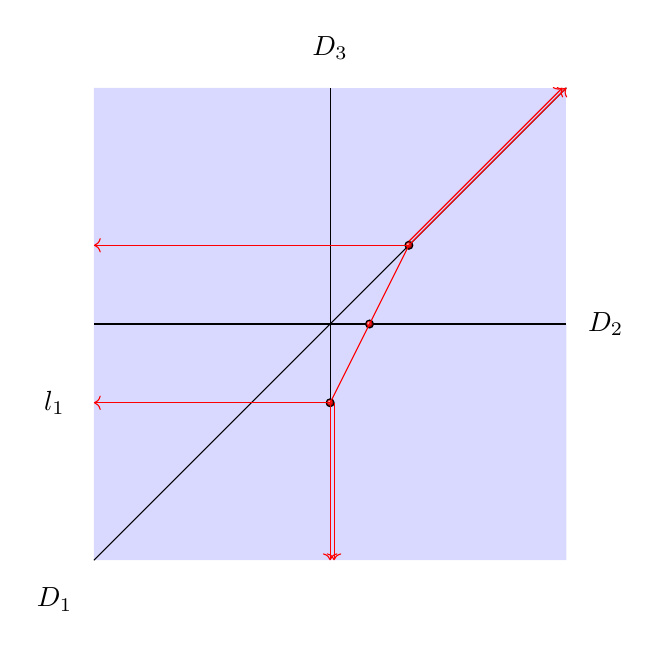
\begin{tikzpicture}
\fill[white!85!blue] (-6,0)--(-3,0)--(-3,3)--(-6,3)--cycle;
\fill[white!85!blue] (-6,0)--(-3,0)--(-3,-3)--(-9,-3)--cycle;
\fill[white!85!blue] (-6,0)--(-9,-3)--(-9,3)--(-6,3)--cycle;
\draw[black] (-6,0)--(-6,3);
%\draw[dashed] (-6,0)--(-9,0);
\draw[black] (-6,0)--(-9,0);
\node at (-6,3.5) {$D_3$};
\draw[black] (-6,0)--(-3,0);
%\draw[dashed] (-6,0)--(-3,3);
\draw[black] (-6,0)--(-3,3);
\node at (-2.5,0) {$D_2$};
\draw[black] (-6,0)--(-9,-3);
%\draw[dashed] (-6,0)--(-6,-3);
\draw[black] (-6,0)--(-6,-3);
\node at (-9.5,-1){$l_1$};
\node at (-9.5,-3.5) {$D_1$};
\draw[ball color=red] (-6,-1) circle (0.5mm);
\draw[ball color=red] (-5.5,0) circle (0.5mm);
\draw[ball color=red] (-5,1) circle (0.5mm);
%\draw[ball color=red] (-5.5,.5) circle (0.5mm);
%\draw[ball color= red] (-5.5,1) circle (0.5mm);
\draw[->,color = red] (-6,-1)--(-6,-3);
\draw[->,color = red] (-5.95,-1)--(-5.95,-3);
\draw[->,color = red] (-6,-1)--(-9,-1);
\draw[-,color = red] (-6,-1)--(-5,1);
%\draw[-,color = red] (-6,-.5)--(-5.75,-.25);
%\draw[-,color = red] (-5.75,-.25)--(-5.625,0);
%\draw[->,color = red] (-5.75,-.25)--(-5.75,-3);
%\draw[-,color = red] (-5.625,0)--(-5.5,.25);
\draw[->,color = red] (-5,1)--(-3,3);
\draw[->,color=red] (-5,1.05)--(-3.05,3);
%\draw[-,color = red] (-5.5,.25)--(-5.5,.5);
%\draw[-,color = red] (-5.5,.5)--(-5.5,1);
%\draw[->,color=red] (-5.5,1)--(-3.5,3);
\draw[->,color=red](-5,1)--(-9,1);
\end{tikzpicture}
\caption{The tropical type $\gamma$
\label{fig1}}
\end{figure}


%\fill[white!85!blue] (-6,0)--(-3,0)--(-3,3)--(-6,3)--cycle;
%\fill[white!85!blue] (-6,0)--(-3,0)--(-3,-3)--(-9,-3)--cycle;
%\fill[white!85!blue] (-6,0)--(-9,-3)--(-9,3)--(-6,3)--cycle;
%\draw[black] (-6,0)--(-6,3);
%%\draw[black] (-6,0)--(-9,0);
%\node at (-6,3.5) {$D_3$};
%\draw[black] (-6,0)--(-3,0);
%%\draw[black] (-6,0)--(-3,3);
%\node at (-2.5,0) {$D_2$};
%\draw[black] (-6,0)--(-9,-3);
%%\draw[black] (-6,0)--(-6,-3);
%\node at (-9.5,-3.5) {$D_1$};
%\draw[ball color= red] (-6,0) circle (0.5mm);
%\draw[ball color = red] (-7,-1) circle (0.5mm);
%\draw[->,color=red] (-7,-1)--(-7,-2.5);
%\draw[->, color=red] (-7,-1)--(-8.5,-1);
%\draw[-,color=red] (-6,0)--(-7,-1);
%\draw[-,color = red] (-6,0)--(-5,0);
%\draw[ball color = red] (-5,0) circle (0.5mm);
%\draw[->, color =red] (-5,0)--(-5,-2.5);
%\draw[->, color = red] (-5,0)--(-4,1);
%%\draw[dashed] (-5,0)--(-3,2);
%\draw[-,color = red] (-6,0)--(-6,1);
%\draw[ball color = red] (-6,1) circle (0.5mm);
%\draw[->, color =red] (-6,1)--(-5,2);
%%\draw[dashed](-6,1)--(-4,3);
%\draw[->, color = red] (-6,1)--(-8.5,1);





\begin{figure}[h]
\centering
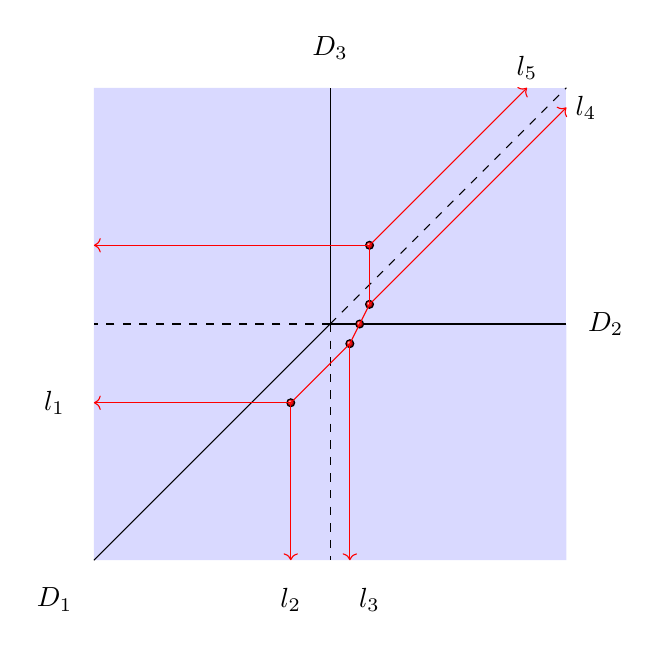
\begin{tikzpicture}
\fill[white!85!blue] (-6,0)--(-3,0)--(-3,3)--(-6,3)--cycle;
\fill[white!85!blue] (-6,0)--(-3,0)--(-3,-3)--(-9,-3)--cycle;
\fill[white!85!blue] (-6,0)--(-9,-3)--(-9,3)--(-6,3)--cycle;
\draw[black] (-6,0)--(-6,3);
\draw[dashed] (-6,0)--(-9,0);
\node at (-6.5, -3.5) {$l_2$};
\node at (-5.5,-3.5) {$l_3$};
\node at (-6,3.5) {$D_3$};
\draw[black] (-6,0)--(-3,0);
\draw[dashed] (-6,0)--(-3,3);
\node at (-2.5,0) {$D_2$};
\node at (-2.75, 2.75) {$l_4$};
\node at (-3.5,3.25) {$l_5$};
\draw[black] (-6,0)--(-9,-3);
\draw[dashed] (-6,0)--(-6,-3);
\node at (-9.5,-1){$l_1$};
\node at (-9.5,-3.5) {$D_1$};
\draw[ball color=red] (-6.5,-1) circle (0.5mm);
%\draw[ball color=red] (-6,-.5) circle (0.5mm);
\draw[ball color=red] (-5.75,-.25) circle (0.5mm);
\draw[ball color=red] (-5.625,0) circle (0.5mm);
\draw[ball color=red] (-5.5,.25) circle (0.5mm);
%\draw[ball color=red] (-5.5,.5) circle (0.5mm);
\draw[ball color= red] (-5.5,1) circle (0.5mm);
\draw[->,color = red] (-6.5,-1)--(-6.5,-3);
\draw[->,color = red] (-6.5,-1)--(-9,-1);
\draw[-,color = red] (-6.5,-1)--(-6,-.5);
\draw[-,color = red] (-6,-.5)--(-5.75,-.25);
\draw[-,color = red] (-5.75,-.25)--(-5.625,0);
\draw[->,color = red] (-5.75,-.25)--(-5.75,-3);
\draw[-,color = red] (-5.625,0)--(-5.5,.25);
\draw[->,color = red] (-5.5,.25)--(-3,2.75);
\draw[-,color = red] (-5.5,.25)--(-5.5,.5);
\draw[-,color = red] (-5.5,.5)--(-5.5,1);
\draw[->,color=red] (-5.5,1)--(-3.5,3);
\draw[->,color=red](-5.5,1)--(-9,1);
%\draw[ball color= red] (-6,0) circle (0.5mm);
%\draw[->,color=red] (-6,0)--(-6,-2.5);
%\draw[->, color=red] (-6,0)--(-8.5,0);
%\draw[-,color = red] (-6,0)--(-5,0);
%\draw[ball color = red] (-5,0) circle (0.5mm);
%\draw[->, color =red] (-5,0)--(-5,-2.5);
%\draw[->, color = red] (-5,0)--(-4,1);
%\draw[dashed] (-5,0)--(-3,2);
%\draw[-,color = red] (-6,0)--(-6,1);
%\draw[ball color = red] (-6,1) circle (0.5mm);
%\draw[->, color =red] (-6,1)--(-5,2);
%\draw[dashed](-6,1)--(-4,3);
%\draw[->, color = red] (-6,1)--(-8.5,1);

\end{tikzpicture}
\caption{The tropical type $\tau'$
\label{fig2}}
\end{figure}








%Writing $l_i$ for the edge length of an edge $e_i$ and $h$ the negative height of the unique vertex contained the legs $l_1,l_2$, it is easy to see that the linear function $l_i$ and $h$ give coordinates for the moduli space $\tau'$, and $\ev^*(P)=h\prod_{i=1}^5l_i$, hence vanishes on the boundary of $\tau$. As a result, the contribution from this graph is $\deg_{\tau}(P) = 1$. 
%
%
%By the tropical correspondence theorem, we know the total integral must evaluate to $1$, hence all other terms on the righthand side of Equation \ref{maineq1} must sum to zero in this case. There are two primary behaviors which yield this vanishing. This first is when $\deg_{\tau'}(P)$ yields a polynomial which yields a vanishing cohomology class. An example of such a $\pmb\tau'$ is depicted in Figure \ref{fig2}:
%
%\begin{figure}[h]
%\centering
%\begin{tikzpicture}
%\fill[white!85!blue] (-6,0)--(-3,0)--(-3,3)--(-6,3)--cycle;
%\fill[white!85!blue] (-6,0)--(-3,0)--(-3,-3)--(-9,-3)--cycle;
%\fill[white!85!blue] (-6,0)--(-9,-3)--(-9,3)--(-6,3)--cycle;
%\draw[black] (-6,0)--(-6,3);
%%\draw[black] (-6,0)--(-9,0);
%\node at (-6,3.5) {$D_3$};
%\draw[black] (-6,0)--(-3,0);
%%\draw[black] (-6,0)--(-3,3);
%\node at (-2.5,0) {$D_2$};
%\draw[black] (-6,0)--(-9,-3);
%%\draw[black] (-6,0)--(-6,-3);
%\node at (-9.5,-3.5) {$D_1$};
%\draw[ball color= red] (-6,0) circle (0.5mm);
%\draw[ball color = red] (-7,-1) circle (0.5mm);
%\draw[->,color=red] (-7,-1)--(-7,-2.5);
%\draw[->, color=red] (-7,-1)--(-8.5,-1);
%\draw[-,color=red] (-6,0)--(-7,-1);
%\draw[-,color = red] (-6,0)--(-5,0);
%\draw[ball color = red] (-5,0) circle (0.5mm);
%\draw[->, color =red] (-5,0)--(-5,-2.5);
%\draw[->, color = red] (-5,0)--(-4,1);
%%\draw[dashed] (-5,0)--(-3,2);
%\draw[-,color = red] (-6,0)--(-6,1);
%\draw[ball color = red] (-6,1) circle (0.5mm);
%\draw[->, color =red] (-6,1)--(-5,2);
%%\draw[dashed](-6,1)--(-4,3);
%\draw[->, color = red] (-6,1)--(-8.5,1);
%
%\end{tikzpicture}
%\caption{
%\label{fig2}}
%\end{figure}
%
%
%This tropical type has a unique tropical lift $\gamma'$, and the maps $\Sigma(\mathscr{M}_{\pmb\gamma})\rightarrow \Sigma(\mathscr{M}_{\pmb\tau}) \rightarrow \Sigma(\mathscr{M}_{0,6})$ induces isomorphism of cones $\gamma' \cong \tau' \cong \mathbb{R}_{\ge 0}^{|E(G_{\tau'})|}$. It follows from this that $deg(P_{\tau'})$ is the quadratic polynomial given by the product of the two PL functions given by the edge lengths $e_1$ and $e_2$. The associated cohomology classes are $c_1(L_{e_1})= -\psi_{e_1,v_{1}}-\psi_{e_1,v}$ and $c_1(L_{e_2})= -\psi_{e_2,v_{2}}-\psi_{e_2,v}$, where $\psi_{e_i,v}$ refers to the $\psi$ class pulled back along the natural map $\mathscr{M}(X,\pmb\tau) \rightarrow \prod_{v \in V(G_{\tau})}\mathfrak{M}_{0,3}$. Since the pullback along the stabilization map $\prod_{v \in V(G_{\tau})} \mathscr{M}_{0,3}$ is trivial, by the standard comparison result for $\psi$-classes, both $\psi_{e_1,v_1} =0$ and $\psi_{e_2,v_2} = 0$, and $\psi_{e_i,v}$ is supported on the locus of curves where the edge $e_i$ is subdivided. But $e_1$ and $e_2$ cannot be both subdivided at the same time, meaning $\psi_{e_1,v}\psi_{e_2,v} = 0$, and $deg(P_{\tau'})[\mathscr{M}_{\tau'}]^{vir} = 0$. 
%
%%It follows as a very special case of various works, including \cite{GaMa} \cite{tropcor},  that this integral may be computed using an appropriate tropical curve count. Equation \ref{maineq1} also yields the tropical approach to evaluating this integral. To see this, consider the modification $p: \tilde{X} \rightarrow X$ given by blowing up all toric fixed points. The resulting cone complex $\Sigma(\tilde{X})$ has six new piecewise quadratic functions $Q_i = E_i\cap  (D_i - E_i - E_{i+1})$ associated with the six $2$-dimensional cones of $\Sigma(\tilde{X})$. Upon pulling these piecewise quadratic functions back to the cohomology of $\tilde{X}$, these are all identified with $p^*[pt]$. Since $p_*[\mathscr{M}(\tilde{X},\beta')]^{vir}=  [\mathscr{M}(X,\beta)]^{vir}$ by the main result of \cite{bir_GW}, the projection formula and Equation \ref{maineq1} combine to show the invariant of \ref{exinv} is given by:
%%\[\int_{[\mathscr{M}(\tilde{X},\beta')]^{vir}} \prod_{i=1}^5ev_{x_i}^*Q_i = \sum_{\pmb\tau'\in S} \int_{[\mathscr{M}(X,\pmb\tau')]^{vir}} 1.\]
%
%%To evaluate the righthand side of the above equation, we first observe that the only tropical curves with tropical moduli of dimension $3$ satisfying the constraint $\ev_{x_11}^*(\pt)\ev_{x_{21}}^*(\pt)\ev_{x_{31}}(\pt)$ is depicted in Figure \ref{fig2}:
%
%
%
%%With the above restriction in mind, we are only dimension $4$ and $5$ tropical types which can contribute are given below:
%%
%%
%%
%%
%%
%%meaning we must compute the pullback $\psi_{e_1,v}\psi_{e_2,v}$ from $\prod_{v \in V(G_{\tau})}\mathfrak{M}_{0,3}$. 
%%Moreover, any one can show that further degenerate tropical type does not induce a smooth tropical evaluation map. As a result, the main theorem reduces the calculation to the following tautological integral:
%%
%%\begin{equation}
%%\int_{[\mathscr{M}(\widetilde{X},\gamma)]^{vir}} c_1(L_{e_2})
%%\end{equation}
%%
%%The corresponding tautological insertion is $c_1(L_{e_2})= -\psi_{e_2,v_{2}}-\psi_{e_2,v}$ and $\psi_{e_i,v}$ refers to the $\psi$ class pulled back along the natural map $\mathscr{M}(X,\pmb\tau) \rightarrow \prod_{v \in V(G_{\tau})}\mathfrak{M}_{0,3}$. Since the pullback along the stabilization map $\prod_{v \in V(G_{\tau})} \mathscr{M}_{0,3}$ is trivial, by the standard comparison result for $\psi$-classes, both $\psi_{e_1,v_1} =0$ and $\psi_{e_2,v_2} = 0$, meaning we must compute the pullback $\psi_{e_2,v}$ from $\prod_{v \in V(G_{\tau})}\mathfrak{M}_{0,3}$. Applying the psi class comparison result, first relating $Stab^*(\overline{\psi}_{e_1,v})$ with $\psi_{e_1,v}$ followed by the comparison between $\psi_{e_1,v}$ on $\mathscr{M}(X,\pmb\tau)$ yields the the virtual class $[\mathscr{M}(X,\pmb\tau')]^{vir}$. Taking degree yields the expected answer of $1$.
%
%The other case is when $\deg_{\tau'}(P)$ is itself the zero polynomial, as happens for $\tau'$ depicted in Figure \ref{fig3}. To see this, observe that the PL functions $P_1$, $P_3$ and $P_4$ are pulled back along $p$. Since $\tau'$ is a cone of dimension $4$, $\deg_{\tau'}(P)= 0$ for any piecewise polynomial of degree less than $4$. The projection formula now yields:
%$$\deg_{\tau'}(P) = P_1P_3P_4\deg_{\tau'}(P_2P_5)=0.$$
%
%
%\begin{figure}[h]
%\centering
%\begin{tikzpicture}
%\fill[white!85!blue] (-6,0)--(-3,0)--(-3,3)--(-6,3)--cycle;
%\fill[white!85!blue] (-6,0)--(-3,0)--(-3,-3)--(-9,-3)--cycle;
%\fill[white!85!blue] (-6,0)--(-9,-3)--(-9,3)--(-6,3)--cycle;
%\draw[black] (-6,0)--(-6,3);
%\node at (-6,3.5) {$D_3$};
%\draw[black] (-6,0)--(-3,0);
%\node at (-2.5,0) {$D_2$};
%\draw[black] (-6,0)--(-9,-3);
%\node at (-9.5,-3.5) {$D_1$};
%\draw[ball color= red] (-7.5,-1) circle (0.5mm);
%\draw[->,color=red] (-7.5,-1)--(-7.5,-2.5);
%\draw[->, color=red] (-7.5,-1)--(-8.5,-1);
%\draw[-,color = red] (-7.5,-1)--(-6,.5);
%\draw[-,color = red] (-6,.5)--(-6,1.5);
%\draw[ball color = red] (-6,.5) circle (0.5mm);
%\draw[-, color = red] (-6,.5)--(-4,.5);
%\draw[->,color = red] (-6,1.5)--(-7.5,1.5);
%\draw[->,color = red] (-6,1.5)--(-5,2.5);
%\draw[ball color=red](-6,1.5) circle (0.5mm);
%\draw[ball color = red](-4,.5) circle (0.5mm);
%\draw[->, color = red] (-4,.5)--(-3,1.5);
%\draw[->, color = red] (-4,.5)--(-4,-1.5);
%\draw[dashed] (-6,0)--(-3,3);
%\end{tikzpicture}
%\caption{
%\label{fig3}}
%\end{figure}

%
%
%Note that if we tried to evaluate the integral by doing a similar calculation starting on $\mathscr{M}(X,\beta)$, uniqueness would fail. Indeed, the curve below satisfies all tropical constraints, but has tropical dimension $5$:
%
%
%
%
%
%The sets $H_i$ defining the collection $S$ of tropical types above are general points in the cone associated with $Q_i$. It now follows from standard argument that $|S| = 1$ and the integral \ref{exinv} evaluates to $1$.
\end{example}
%
%\begin{remark}
%Similar phenomenon appeared by Maulik and Ranganathan in \cite{degen}, where a splitting formula is studied in the expansion framework for log GW/DT/PT. However, the ...
%\end{remark}





%The theorem above addresses two aspects in which log Gromov-Witten theory changes under log \'etale modifications. First, in the setting of punctured log Gromov-Witten theory, if we have a pair of tropical types $\gamma$ and $\tau$ which are related by stabilization, i.e. stabilization induces $st: \mathscr{M}(\widetilde{X},\gamma) \rightarrow \mathscr{M}(X,\tau)$, we might have $vdim\text{ }[\mathscr{M}(\widetilde{X},\gamma)]^{vir} > dim\text{ }[\mathscr{M}(X,\tau)]^{vir}$. While the main result of \cite{pbirinv} relates the associated log Gromov-theories, it does not explicitly describe the pushforward of log Gromov-Witten classes of $\widetilde{X}$ in terms of log Gromov-Witten classes of $X$. Secondly, even in the the non-punctured setting, the space of insertions for $\widetilde{X}$ is larger with respect to $X$,  and it is natural to ask for whether integrals against this larger space of insertions can be expressed in terms of the smaller space of insertions pulled back from $X$. Since all new cohomology classes on a logarithmic modification $\widetilde{X}$ of $X$ are expressed in terms of piecewise polynomials on the tropicalization $\Sigma(\widetilde{X})$, Theorem \ref{mthm1} establishes that as long as we enlarge our space of insertions to include all tautological classes associated with the log structure on $\mathscr{M}(X,\pmb\tau)$, the space of insertions essentially stabilizes after pushforward. 


%\begin{corollary}
%For $\alpha \in H^{vir\text{ }dim\text{ }\mathscr{M}(\widetilde{X},\pmb\gamma)}(\mathscr{M}(\widetilde{X},\pmb\gamma))$, we have
%
%\[deg\text{ }\alpha \cap [\mathscr{M}(\widetilde{X},\pmb\gamma)]^{vir} = \sum_{\pmb\gamma \subset \pmb\gamma'} st_*(\frac{\alpha}{|Aut(\gamma'/\gamma)|P_{\gamma'}m_{\gamma'}})[\mathscr{M}(X,\pmb\tau)]^{vir}\]
%
%\end{corollary}


%Turning to applications of the formula, we note that relations in log Gromov-Witten theory for a pair $(X,D) typically only appear for invariants appearing on log \'etale modifications $(\tilde{X),\tilde{D})$. In genus $0$, one example of this is the WDVV relation. By construction,  



We provide two primary applications of Equation \ref{maineq1}. 

\subsection{Log-orbifold correspondence for canonical wall structures}

In the setting of mirror symmetry and canonical wall structure for log Calabi-Yau pairs, Gross and Siebert in \cite{scatt} use realizable tropical types referred to as ``wall types" and ``broken line types" to define the necessary enumerative input to construct the canonical wall structures for a log Calabi-Yau pair. Separately, You in \cite{orbBL} constructs analogues of these broken line invariants using orbifold Gromov-Witten theory, later using these invariants in \cite{yougamma} to study the Gamma conjecture for Fano varieties. We use Theorem \ref{mthm1} to compare these invariants. Namely, we use Theorem \ref{mthm1} to provide an alternate description the broken line/wall type invariants as integrals on the space of log maps to a log \'etale modification, from which the log-orbifold correspondence of \cite{BNR2} will allow us to deduce the following corollary:


\begin{corollary}[Proposition \ref{blorb}, Proposition \ref{worb}]
For a log Calabi-Yau pair $(X,D)$ in the sense of \cite{scatt} with essential skeleton $B \subset \Sigma(X)$, $p \in B$ an integral point, and $x \in \sigma_x \subset B$ a general point of a cone $\sigma_x$, the broken-line expansions $\vartheta_{p,x}$ is equal to the orbifold theta-function $\vartheta_{p}(x)$ of \cite{orbBL} of a suitable log \'etale model $\widetilde{X}$ of $X$. Additionally, the canonical wall structure can be expressed using the orbifold Gromov-Witten theory of log \'etale modifications of $X$. 
\end{corollary}


The pairs $(X,D)$ considered in \cite{scatt} satisfy the condition that $D$ contains a zero dimensional stratum. However, the definitions for broken lines expansions given as a result of the above corollary extends to general log Calabi-Yau pairs without the existence a zero dimensional stratum. We show that this assignment extends to a morphism of algebras:

\begin{theorem}[Theorem \ref{blhom}]
For $(X,D)$ a log Calabi-Yau pair in the sense of \cite{int_mirror} and $x \in \sigma_x \subset B(X)$ general, and $\kk[Q] = \kk[NE(X)]/I$ for $I$ a monomial ideal of $\kk[NE(X)]$ such that only finitely many curve classes are not contained in $I$, the assignment sending a theta function $\vartheta_p$ to its associated broken line expansion $\vartheta_{p,x}$ extends to a morphism of $\kk[Q]$ algebras $R_{(X,D)} \rightarrow \kk[\sigma_{x,\NN}^{\gp}][Q]$, with the constant term of a product of broken line expansions given by a descendent log Gromov-Witten invariant.
\end{theorem} 
As in \cite{logWDVV}, the necessary relations required for the result are naturally expressed in terms of invariants on log \'etale modifications of $X$, but yield interesting relations among punctured log Gromov-Witten classes on $X$ by Theorem \ref{mthm1}, generalizing \cite[Theorem $6.1$]{scatt} to the general log Calabi-Yau setting. 

When $X\setminus D$ is an affine log Calabi-Yau which admits a compactification to a Fano variety $X'$, the descendent log Gromov-Witten invariants appearing as the constant term in products of broken line expansions are related to the quantum periods of $X'$ by \cite[Theorem $1.1$]{qpint}. As a result, we produce power series which are weak mirrors to Fano compactifications of $X\setminus D$:

\begin{corollary}\label{fanocor}
For a smooth Fano variety $X$ and $D = D_1+\cdots+D_m \in |-K_X|$ satisfying the conditions of \cite[Theorem $1.1$]{qpint} with $X\setminus D$ having essential skeleton $B$, for any $x \in B$ general with integral tangent space $\Lambda_x$, there is a power series $W_{D,x} \in \kk[\Lambda_x][[NE(X)]]$ which is a weak Landau-Ginzburg mirror to $X$. 
\end{corollary}

\subsection{Log Gromov-Witten theory of split toric bundles}

A second application is in the study of the log Gromov-Witten theory of split toric bundles. Such spaces arise as log \'etale modifications $X \rightarrow S$, with $S$ having generic non-trivial log structure. Theorem \ref{mthm1} can be used to express the punctured log Gromov-Witten theory of $X$ in terms of the punctured log Gromov-Witten theory of $S$. 


\begin{theorem}\label{mthm2}
Given a smooth projective variety $S$ equipped with an snc divisor and any split toric bundle $X \rightarrow S$, the punctured log Gromov-Witten classes of $X$ can be effectively reconstructed in terms of the punctured log Gromov-Witten classes of $S$. In particular, the punctured log Gromov-Witten classes of $X$ push forward to tautological classes in the Chow ring of moduli space of stable curves if the punctured log Gromov-Witten classes of $S$ push forward to tautological classes. 
\end{theorem}

The special case when $S$ has trivial log structure states that the punctured log Gromov-Witten theory of a toric bundle over $S$ can be reconstructed in terms of the absolute Gromov-Witten theory of $S$. When $S = \Spec \kk$, this recovers the results of Molcho and Ranganathan in \cite{logint} and Ranganthan and Urundolil Kumaran in \cite{DRtoric}. The authors of \cite{DRtoric} relate the log Gromov-Witten classes of a toric variety to explicit expressions involving piecewise polynomial classes and the toric contact cycle on the moduli space of stable curves. In our setting, we will require a generalization of the toric contact cycle. Such a generalization is naturally expressed using punctured log Gromov-Witten theory, and we refer to this class as the \emph{toric contact cycle with target log variety}. The following theorem shows that these punctured log Gromov-Witten classes are explicitly expressed in terms of the log Gromov-Witten classes of $S$:

\begin{theorem}[Theorem \ref{hrankt}]\label{mthm3}
For a log smooth projective variety $S$, $\pmb\tau$ a decorated realizable tropical type with a single vertex $v \in V(G_{\tau})$ and $k$ legs with total curve class $\textbf{A} \in H_2(S)$, line bundles $L_1,\ldots,L_k \in Pic(S)$, and vectors $a_i \in \ZZ^{k}$ with $\sum_i a_{ij} = L_j\cdot \textbf{A}$ for all $L_j$, let $[DR_{(L_i,a_i),\textbf{A}}(S,\pmb\tau)] \in A_*(\mathscr{M}(S,\pmb\tau))$ be the associated toric contact cycle with target log variety defined in Equation \ref{drlogt}. Then $[DR_{(L_i,a_i),\textbf{A}}(S,\pmb\tau)]$ is a rational linear combination of log Gromov-Witten classes of $\mathscr{M}(S,\pmb\tau)$. 
\end{theorem}

%More precisely, after slight alternations of the log structure which effect the log Gromov-Witten theory in a way which is immaterial for our purpose, the projection morphism can realized as a log \'etale morphism. 

The proof of Theorem \ref{mthm3} follows by an induction on the number of line bundles $k$. Crucial to carrying out the induction is that the base $S$ is allowed to have log structure and $\pmb\tau$ is allowed to have non-trivial tropical moduli. When the log structure is trivial and $k=1$, we will show that this cycle recovers the double ramification cycle with target, which has an explicit formula given in \cite{DRtarget}. More generally, by appropriately adapting arguments of Molcho from \cite{BNtaut}, we produce an expression for the double ramification cycle with log target which is sufficient to prove Theorem \ref{mthm3} by induction on $k$.

%\begin{remark}
%We expect a yet to be developed theory of localization for punctured log Gromov-Witten theory should also yield Theorem \ref{mthm2}. Nonetheless, the expression we provide which proves Theorem \ref{mthm2} are unlikely to come directly from a general theory of localization, which we expect will
%\end{remark}

%We conclude with remarks on applications of Theorem \ref{mthm3} to the question of reconstructing the punctured log Gromov-Witten theory of an snc pair $(X,D)$ from the absolute Gromov-Witten theory of all strata. Such a result was established in recent work of Maulik-Ranganathan in the unpunctured setting, and op. cit. further conjectures a generalized reconstruction result for punctured log Gromov-Witten invariants. We use their results in consort with Theorem \ref{mthm3} to partially verify this conjecture. Important input comes from the gluing formula of \cite{toricglue}. We expect a more widely applicable gluing scheme should yield the conjecture in general. 

\subsection{Future direction}
%An effective use of Equation \ref{mthm1} requires an understanding of the singularities of the tropical moduli space of tropical maps to $\Sigma(X)$. It is conceivable that more effective formulas can be found after passing to a sufficient subdivision so that the refined virtual class of \cite{BNR2} can be used. 

The strategy used to produce Equation \ref{maineq1} work more broadly for providing formulae for the pushforward of piecewise polynomial classes on log \'etale modifications. Many structures and tools available in Gromov-Witten theory (gluing, localization, Givental formalism) are only expected to become available after a sufficient log \'etale modification of the moduli spaces in log Gromov-Witten theory. The tools for producing Equation \ref{maineq1} should offer a pathway of transporting such structures and tools to the study of intersection theory on a fixed log \'etale model of the moduli stack of log stable maps.

Finally, Maulik and Ranganathan in the recent preprint \cite{MRrecon} use degenerations and the expanded formalism for log Gromov-Witten theory to prove a reconstruction result for the log Gromov-Witten theory of simple normal crossings pairs $(X,D)$ in terms of the absolute Gromov-Witten theory of all strata. One key ingredient to extending this result to the setting of punctured log maps is understanding spaces of maps into targets with generically non-trivial log structure. An important development in this direction is Theorem \ref{mthm3}. The author expects these two works, together with slight improvements to the gluing schemes for punctured log curves, should yield a similar reconstruction result for the entire punctured log Gromov-Witten theory for a simple normal crossings pair, providing an affirmative answer to a question posed by Maulik and Ranganathan in \cite{MRrecon}. 

\subsection{Acknowledgement}
I would like to thank Robert Crumplin, Mark Gross, Ajith Kumaran, Xuanchun Lu, Davesh Maulik, Dhruv Ranganathan and Peter Zaika for many helpful discussions related to this work. I would especially like to thank Dhruv Ranganathan who suggested the approach taken to establish the $k=1$ case of Theorem \ref{mthm3}. The author is supported by NSF DMS-2502976.


\section{Logarithmic and tropical preliminaries}

Throughout this paper, given a fan $\Sigma$ in $\mathbb{R}^n$, we refer to the associated toric variety as $Z_{\Sigma}$. If $\sigma$ is a cone and $\sigma'\subset \sigma$ is a lattice coarsening, there is an associated root stack of $Z_\sigma$ associated with $\sigma'$, which we denote by $Z_{\sigma'}$. We recall the definitions and constructions surrounding Artin fans which will be invoked in this paper:

\begin{definition}
For $\sigma$ a rational polyhedral cone, the Artin cone  $\mathcal{A}_{\sigma} = [Z_{\sigma}/T_{\sigma}]$ is the global quotient of the toric variety $Z_{\sigma}$ by its dense algebraic torus. An Artin fan is a logarithmic algebraic stack with a strict \'etale cover by Artin cones.

For a face $\omega \subset \sigma$, let $Z_{\sigma,\omega}$ be the closure of the torus stratum in $Z_\sigma$ associated with the interior of the cone $\omega$, and we define the associated idealized Artin cone $\mathcal{A}_{\sigma,\omega}$ to be the stack quotient $[Z_{\sigma,\omega}/T_{\sigma}]$. 
\end{definition}


Artin fans give a useful method for faithfully embedding a category of tropical objects into the category of algebraic stacks, as the following theorem makes precise:

\begin{theorem}[\cite{stacktrop} Theorem $6.11$]
There is an equivalence of $2$-categories between the categories of Artin fans and cone stacks. For a cone $\sigma$, the equivalence is given by sending $\sigma$ to $\mathcal{A}_\sigma$. 
\end{theorem}
By the theorem above, for any subdivision or lattice coarsening of a cone stack $\widetilde{\Sigma} \rightarrow \Sigma$, there is a corresponding morphism of Artin fans $\mathcal{A}_{\widetilde{\Sigma}} \rightarrow \mathcal{A}_{\Sigma}$, and we refer to the morphism on either side of the equivalence as a subdivision or lattice coarsening. The corresponding morphism of Artin fans is proper and log \'etale by \cite[Theorem $2.4.1$]{bir_GW}.

The data of an fs log scheme $X$ is given by a map to Olsson's stack of log structure $X \rightarrow Log$. We define an Artin fan for $X$ to be any Artin fan $\mathcal{X}$ such that $X \rightarrow Log$ admits a factorization through the natural map $\mathcal{X} \rightarrow Log$. Moreover, given a log \'etale morphism $\widetilde{\mathcal{X}} \rightarrow \mathcal{X}$ induced by subdivisions or lattice coarsenings, we may construct a log \'etale modification or more generally log \'etale alteration $\widetilde{X} \rightarrow X$ given by pulling back the log \'etale morphism of Artin fans. 


While the canonical assignment of an Artin fan to an fs log stack in \cite[Proposition $3.2.1$]{bound} fails to be functorial, there nonetheless exists a functor, constructed in \cite[Appendix $C$]{punc}, from the category fs log stacks (and more generally fine log stacks) to the category of \emph{generalized cone complexes}, as defined in \cite[$\S 2.2$]{ACP}. For $\Sigma$ a generalized cone complex we denote by $PL(\Sigma)$ the $\mathbb{R}$ vector space of piecewise linear functions on $\Sigma$, and $PP(\Sigma)$ the space of piecewise polynomial functions. Note that we have a map $Sym^*(PL(\Sigma)) \rightarrow PP(\Sigma)$, but this map is not typically surjective. However, this map is surjective for a simple log algebraic stacks, and every log smooth stack has a log \'etale model which is a simple log algebraic stack, see \cite[Lemma $3.6$]{intDR}. When a smooth log scheme $X$ is induced by a simple normal crossings divisor $D = D_1+\cdots+D_k$, a component $D_i$ induces a piecewise linear function on $\Sigma(X)$ which has slope $1$ along the ray associated with $D_i$ and $0$ along all other rays. We also denote by $D_i \in PL(\Sigma(X))$ the PL function associated with $D_i$, with context distinguishing these uses. 


\subsection{Punctured log Gromov-Witten Theory}
We now fix a log smooth morphism $X \rightarrow B$, where $B$ is either log smooth over a $\Spec\kk$ for $\kk$ an algebraically closed field of characteristic $0$ or the standard log point $\Spec \kk^{\dagger} = (\Spec\kk,\NN)$, with Artin fans $\mathcal{A}_X$ and $\mathcal{A}_B$. For $\sigma \in \Sigma(X)$, we define $\sigma_{\NN}$ the set of integral points of $\sigma$ and $\sigma_{\NN}^{\gp}$ the collection of integral tangent vectors at any point of $\sigma \setminus \partial \sigma$. Finally, for a generalized cone complex $\Sigma$, define $\Sigma^{[k]}$ to be the collection of $k$-dimensional cones of $\Sigma$, $\Sigma(\NN) = \cup_{\sigma\in \Sigma} \sigma_{\NN}$ and $\Sigma(\ZZ) = \cup_{\sigma \in \Sigma} \sigma_{\NN}^{\gp}$. For either a cone $\sigma \in \Sigma(X)$ or a point $p \in \sigma\setminus \partial \sigma$, we let $X_{\sigma}$ or $X_p$ refer to closure of the stratum with generic point mapping to the point of $\mathcal{A}_X$ associated with the cone $\sigma$. 

We will primarily study the enumerative geometry of log smooth pairs $(X,D)$ in this paper using punctured log Gromov-Witten theory. Developed originally by Abramovich, Chen, Gross and Siebert in \cite{punc}, this is a more flexible framework for the studying the relative Gromov-Witten theory of log smooth morphisms $X \rightarrow B$, in particular providing a useful way of recursively describing the boundary of moduli spaces of log stable maps. The primary input yielding this additional flexibility comes from tropical geometry.

More precisely, along with fixing genus and degrees in specifying moduli spaces of log stable maps, we will also fix the data of a \emph{realizable tropical type}. This comes from the data of a PL map $\Gamma_{\tau} \rightarrow \Sigma(X)$ from a source meterized graph with legs $\Gamma_{\tau}$ to $\Sigma(X)$. Letting $G_{\tau}$ be the abstract graph associated to $\Gamma_{\tau}$, such a map defines contact orders $u(l),u(e) \in \Sigma(X)(\ZZ)$ for all legs $l \in L(G_{\tau})$ and edges $e \in E(G_{\tau})$, and target cones $\pmb\sigma(v) \in \Sigma(X)$ for all vertices $v \in V(G_{\tau})$. In addition, for any realizable tropical type $\tau$, \cite{punc} provides a monoid whose dual is a cone which will also be denoted by $\tau$ which is the base of the universal family of tropical maps of type $\tau$. More precisely, for any family of tropical maps $\Gamma/\omega \rightarrow \Sigma(X)$ of type $\tau$ parameterized by a base cone $\omega$, there exits a unique integral linear map $\omega \rightarrow \tau$ such that the family over $\omega$ is pulled back from the universal family over $\tau$. Given another tropical type $\tau'$, we say that $\tau'$ is marked by $\tau$ if there is a face $\tau \subset \tau'$ such that the restriction of the universal family over $\tau'$ to the face $\tau$ yields the universal family over $\tau$. For a simple normal crossings pair \footnote{\cite{punc} defines types of punctured log maps in larger generality in the presence of monodromy in the log structure. For our purposes, defining such types in the setting of simple normal crossings pairs suffices.}, we further consider combinatorial types $\beta$ of punctured log map in which we specify only the total curve class $\textbf{A}$, genus $g$, and the tangency conditions $u(l) \in \pmb\sigma(l)^{\gp}_{\NN}$ of legs. We say a tropical type $\pmb\tau$ is marked by $\beta$ if $\sum_{v \in V(G_{\tau}} \textbf{A}(v) = \textbf{A}$, $\sum_{v \in V(G_{\tau})} g(v) = g$, and the tangency conditions of the legs of $\tau$ agree with those specified by $\beta$. 


Additionally, letting $M$ be a monoid of effective curve classes, we consider decorations $g: V(G_{\tau}) \rightarrow \NN$ and $\textbf{A}: V(G_{\tau}) \rightarrow M$ of the vertices of the graph $G_{\tau}$ with genus and curve classes respectively. We call a tropical type with this additional data a decorated tropical type, which we denote by $\pmb\tau$. A decorated tropical type $\pmb\tau$ specifies moduli spaces $\mathscr{M}(X,\pmb\tau)$ and $\mathfrak{M}(\mathcal{X},\pmb\tau)$ of punctured log maps marked by the type $\tau$ with targets $X$ and $\mathcal{X}$ respectively. For the purpose of gluing, it will also be necessary to consider the stack $\mathfrak{M}^{\ev}(\mathcal{X},\pmb\tau) = \mathfrak{M}(\mathcal{X},\pmb\tau) \times_{\prod_{l \in L(G_{\tau})}\mathcal{X}_{\pmb\sigma(l)}} X_{\pmb\sigma(l)}$. Finally, for a realizable tropical type $\pmb\tau$, we refer to the punctured log Gromov-Witten classes of $\mathscr{M}(X,\pmb\tau)$ as classes of the form $\alpha\cap[\mathscr{M}(X,\pmb\tau')]^{\vir}$ for $\pmb\tau'$ a decorated tropical type marked by $\pmb\tau$ and $\alpha \in A^*(\mathscr{M}(X,\pmb\tau))$ operational Chow classes given as polynomials in tautological classes, in the sense of \cite{tauttarget} pulled back along $\mathscr{M}(X,\pmb\tau') \rightarrow \mathscr{M}(X)$ which forgets log structures. 




% in pulled back along evaluation maps of operational Chow classes on strata of $X$ and tautological classes pulled back along the forgetful map $\mathscr{M}(X,\pmb\tau) \rightarrow \mathfrak{M}_{g,n}$ to the moduli space of prestable maps.




\section{Log Gromov-Witten invariants of $\tilde{X}$ from log Gromov-Witten invariants of $X$}

Letting $X \rightarrow B$ be as in the previous section, we consider $X$ equipped with it's relative Artin fan $X \rightarrow\mathcal{X} = \mathcal{A}_X \times_{\mathcal{A}_B} B$, and suppose we have a log \'etale modification $\pi: \widetilde{X}\rightarrow X$ pulled back from a subdivision and lattice coarsening of Artin fans $\widetilde{\mathcal{A}}_X \rightarrow \mathcal{A}_X$. Letting $\Sigma(\widetilde{X})\rightarrow \Sigma(X)$ be the corresponding morphism in rational polyhedral cone complexes, consider a realizable tropical type $\gamma$ of punctured tropical map $\Gamma_\gamma \rightarrow \Sigma(\widetilde{X})$. We recall from \cite{pbirinv} the notion of a tropical lift:

\begin{definition}[\cite{pbirinv} Definition $4.1$]\label{dtlift}
Suppose we have realizable tropical types $\gamma$ and $\tau$ of punctured tropical maps to $\Sigma(\widetilde{X})$ and $\Sigma(X)$ respectively. Then $\gamma$ is a tropical lift of $\tau$ if there exists an inclusion of cones $i: \gamma \rightarrow \tau$ not factoring through a strict face inclusion $\tau' \subset \tau$ and a puncturing of the family of tropical curves $\overline{\Gamma}^\circ\subset \overline{\Gamma}_{\gamma}$ over the cone $\gamma$ induced by $i$ which is contained in the domain of definition of the punctured tropical map $(\overline{\Gamma}_{\gamma}^{\circ}/\gamma,f)$ with target $\Sigma(X)$ induced by $i$ such that the universal family of punctured tropical maps over $\gamma$ is given by $\overline{\Gamma}^\circ \times_{\Sigma(X)} \Sigma(\tilde{X}) \rightarrow \Sigma(\widetilde{X})$ in the category of rational polyhedral cone complexes.

A decorated tropical type $\pmb\gamma$ is a \emph{decorated lift} of a decorated tropical type $\pmb\tau$ if the underlying tropical type $\gamma$ is a tropical lift of the underlying type $\tau$, and after applying the morphism $\pi_*:H_2(\widetilde{X}) \rightarrow H_2(X)$ to the decoration of $\gamma$, the resulting decorated tropical type of map to $\Sigma(X)$ is marked by $\pmb\tau$. 
\end{definition}



We have a corresponding moduli space of log stable maps $\mathscr{M}(\widetilde{X}/B,\gamma)$, and by \cite[Theorem $4.6$]{pbirinv} the space is non-empty only if $\gamma$ is a tropical lift of some tropical type $\tau$ of a punctured tropical map $\Gamma_{\tau} \rightarrow \Sigma(X)$. If we additionally enhanced $\gamma$ to a decorated tropical type $\pmb\gamma$, then $\pmb\gamma$ is the lift of a unique decorated tropical type $\pmb\tau$, and stabilization induces a morphism of moduli stacks $\mathscr{M}(\widetilde{X}/B,\pmb\gamma) \rightarrow \mathscr{M}(X/B,\pmb\tau)$. In this setting, we recall the decorated version of the main theorem of \cite{pbirinv}, as well as a corollary which holds under an additional assumption on $\gamma$:




\begin{theorem}\label{decthm}
For a decorated tropical type $\pmb\gamma$ lifting the decorated tropical type $\pmb \tau$, denote by $\mathscr{M}_{\pmb\tau}$ the image of $\mathscr{M}(\widetilde{X}/B,\pmb\gamma) \rightarrow \mathscr{M}(X/B,\pmb\tau)$. Then $\mathscr{M}_{\pmb\tau}$ is a union of connected components of $\mathscr{M}(X/B,\pmb\tau)$, and there exists a proper log \'etale morphism $\mathfrak{M}_{\gamma\rightarrow \tau} \rightarrow \mathfrak{M}_{\tau}$ such that the following diagram is cartesian:

\begin{equation}\label{cart}
\begin{tikzcd}
\mathscr{M}(\widetilde{X}/B,\pmb\gamma) \arrow{r} \arrow{d} & \mathfrak{M}_{\gamma \rightarrow \tau} \arrow{d} \\
\mathscr{M}_{\pmb\tau} \arrow{r} & \mathfrak{M}_{\tau}.
\end{tikzcd}
\end{equation}
Moreover, the relative perfect obstruction theories attached to the horizontal morphisms are related via pullback.
\end{theorem}



\begin{corollary}\label{puncmcr1}
Suppose $\gamma$ is a lift of $\tau$, and dim $\tau =$ dim $\gamma$. Let $m = \coker|\gamma^{\gp} \rightarrow \tau^{\gp}|$. Then for $s: \mathscr{M}(\widetilde{X}/B,\gamma) \rightarrow \mathscr{M}(X/B,\tau)$ the map induced by $\pi: \widetilde{X} \rightarrow X$: 

\[s_*[\mathscr{M}(\widetilde{X}/B,\pmb\gamma)]^{\vir} = \frac{1}{m}[\mathscr{M}_{\pmb\tau}]^{\vir} .\] 
\end{corollary}
Note that if the decorations are both taken in the monoids $H_2^+(X)$ and $H_2^+(\widetilde{X})$ of effective curve classes in Theorem \ref{decthm}, we have $\mathscr{M}_{\pmb\tau}  =\mathscr{M}(X/B,\pmb\tau)$. To ease notational burden in this section, we will typically write $\mathscr{M}(X/B,\pmb\tau) = \mathscr{M}(X,\pmb\tau)$. 




%In order to express log Gromov-Witten invariants of $\widetilde{X}$ in terms of log Gromov-Witten invariants of $X$, we observe that we may understand a Chow class $\alpha \in A_*(\widetilde{X})$ in terms of $A_*(X)$ and piecewise polynomials on $\Sigma(\widetilde{X})$:

%\begin{lemma}\label{insert}
%The map $\beta: A_*(X)\otimes Sym(PL(\Sigma(\widetilde{X}))) \rightarrow A_*(\widetilde{X})$ defined by $\beta(\alpha\otimes P) = f^*(\alpha)\cap P$ is surjective. 
%\end{lemma}

%\begin{proof}
%We first assume $\widetilde{X}$ is smooth and $\widetilde{X} \rightarrow X$ is the composite of a sequence of blowups along regular centers, which can be assumed after replacing $\widetilde{X}$ with a further modification. Moreover, by repeatedly applying the Lemma in the case of a single blowup, we reduce the statement of the Lemma in the above setting to the case of a single blowup. Letting $\tilde{S}$ be the exceptional divisor of $p: \widetilde{X} \rightarrow X$ mapping down to $S$, by \cite{Fulint} Proposition $6.7(e)$, we have the natural map $A_*(X)\oplus A_*(\widetilde{S}) \rightarrow A_*(\widetilde{X}) = A^{dim\text{ }X-*}(\widetilde{X})$ is surjective. Moreover, for $p: \widetilde{S} \rightarrow S$ the blowdown morphism, $p$ is a projection from a projective bundle, and by \cite{Fulint} Theorem $3.3(b)$, any element in $A_*(\widetilde{S})$ can be uniquely written in the form:

%\[\alpha = \sum_{j=0}^{\text{codim}(S)-1} c_1(\mathcal{O}(1))^jp^*\alpha_j,\]
%for classes $\alpha_j \in A^*(S)$. The class $c_1(\mathcal{O}(1))$ is pulled back from a cohomology class on $\mathcal{A}_{\widetilde{X}}$ associated with a piecewise linear function $P$ on $\Sigma(\widetilde{X})$. Hence, letting $i: S \rightarrow X$ and $\tilde{i}: \tilde{S}\rightarrow \widetilde{X}$ be the inclusions, we have:
%\[\tilde{i}_*\alpha = \sum_{j=0}^{\text{codim}(S)-1} \tilde{i}_*(\tilde{i}^*(c_1(\mathcal{O}(1))^j)p^*\alpha_j) = \sum_{j=0}^{codim(S)-1} P^j\cap \tilde{i}_*p^*\alpha_j = \sum_{j=0}^{\text{codim}(S)-1} P^j\cap p^*i_*\alpha_j.\]
%Hence, every element in the image of $\tilde{i}: A_*(\tilde{S}) \rightarrow A_*(\tilde{X})$ is in the image of the map $\beta$, and the desired conclusion follows.

%To remove the assumption that $\widetilde{X} \rightarrow X$ is a composite of blowups, we let $\widetilde{X}' \rightarrow \widetilde{X}$ be a further log \'etale modification such that $\widetilde{X}'\rightarrow X$ is a composite of blowups. Observe that we have the commuting diagram:
%\[\begin{tikzcd}
%A_*(X)\otimes Sym(PL(\Sigma(\widetilde{X}'))) \arrow{r} \arrow{d} & A_*(\widetilde{X}')\arrow{d}\\
%A_*(X)\otimes Sym(PL(\Sigma(\widetilde{X}))) \arrow{r} & A_*(\widetilde{X})
%\end{tikzcd}\]
%The left and right vertical arrows are induced by pushforward on piecewise linear functions along the subdivision $\Sigma(\widetilde{X}') \rightarrow \Sigma(\widetilde{X})$ and pushforward along $A_*(\widetilde{X}') \rightarrow A_*(\widetilde{X})$ respectively. We note in addition that both vertical morphisms are surjective. Since we have seen previously that the top horizontal morphism is surjective, it follows that the bottom horizontal morphism must also be surjective, as required. 

% we note that given any modification $p': \widetilde{X}' \rightarrow X$, there is a further modification $q: \widetilde{X} \rightarrow \widetilde{X}'$ given by a sequence of blowups such that the composite $p: \widetilde{X} \rightarrow X$ is given by sequences of blowups. For any $\alpha \in A_*(\widetilde{X}')$, we consider $q_*\alpha \in A_*(\widetilde{X})$. We now from above that $q_*\alpha = \sum_i p^*\alpha_i\cap P_i$ for $P_i$ a product of cohomology classes associated with piecewise linear functions on $\Sigma(\widetilde{X})$. By \cite{fulton} Proposition $6.7(b)$, we have $\alpha = q_*q^*\alpha$. Since $p_*\alpha_i\cap P_i = \alpha \cap p_*(P_i)$, and $p_*(P_i)$ is a product of piecewise linear functions on $\Sigma(X)$, combining the two previous equalities yields the desired result.

%\end{proof}



%Using Lemma \ref{insert}, for any cohomology class $\alpha \in A^*(\widetilde{X})$, the corresponding class in Chow homology $\alpha \cap [\widetilde{X}]$ can be written as a sum of classes of the form $p^*(\alpha')\cap P$ for $P_i$ a piecewise monomial function on $\Sigma(\widetilde{X})$. As a result, Theorem \ref{mthm1} would facilitate the evaluation of all punctured log Gromov-Witten invariants of $\widetilde{X}$ in terms of the punctured log Gromov-Witten invariants via the projection formula, and Corollary \ref{mcr1} would follow. We therefore turn our attention to the proof of Theorem \ref{mthm1} for the remainder of this section. 


To prove Theorem \ref{mthm1}, we wish to pullback piecewise polynomial functions $P_i \in PP(\Sigma(X))$ to piecewise polynomial functions on $\Sigma(\mathscr{M}(X,\pmb\gamma))$. However, letting $X_s$ be the stratum of $(X,D)$ determined by the contact order of the marked point $x$, the evaluation morphism of algebraic stacks $\ev_x: \mathscr{M}(X,\pmb\gamma) \rightarrow X_s$ typically does not admit an enhancement to a morphism of log stacks. As constructed in \cite{DRtoric}, we modify the log structure on $X_s$ to allow for this as follows: 




First, consider the ghost sheaf $\overline{\mathcal{M}}_{X_s}$ of the log structure on $X_s$. This has global sections given by PL functions on the cone complex $\Sigma(X_s) = \text{Star}(\sigma_s)$. Letting $\sigma_s \in \Sigma(X)$ be the cone associated with the stratum $X_s$, define $\Sigma_{\sigma_s}$ to be the cone complex with cones of the form $q(\sigma) \subset \sigma^{\gp}/\sigma_s^{\gp}$ for $q: \sigma^{\gp} \rightarrow \sigma^{\gp}/\sigma_s^{\gp}$ the quotient map, and note we have a natural quotient map $q: \Sigma(X_s) \rightarrow \Sigma(X_s)_{\sigma_s}$. After identifying $\Gamma(\overline{\mathcal{M}}(X_s))$ with PL functions on $\Sigma(X_s)$, we let $\overline{\mathcal{M}}' \subset \overline{\mathcal{M}}_{X_s}$ be the subsheaf with local sections associated with partial PL functions on $\Sigma(X_s)$ which are pulled back from $\Sigma(X_s)_{\sigma_s}$ along $q$. Define the sub log structure $\mathcal{M}'_{X_s} := \overline{\mathcal{M}}' \times_{\overline{\mathcal{M}}_{X_s}} \mathcal{M}_{X_s}$, with structure morphism $\alpha': \mathcal{M}' \rightarrow \mathcal{O}_{X_s}$ given by restricting $\alpha: \mathcal{M}_{X_s} \rightarrow \mathcal{O}_{X_s}$, and call the resulting fs log scheme $X_s'$. We note there is a log morphism $X_s \rightarrow X_s'$ induced by the inclusion of log structures $\mathcal{M}'_{X_s} \subset \mathcal{M}_{X_s}$. 

To construct an enhancement of the morphism $\ev_x: \mathscr{M}(X,\pmb\gamma) \rightarrow X_s$ to a log morphism $\ev_x: \mathscr{M}(X,\pmb\gamma) \rightarrow X_s'$ for $x$ a marked point of the tropical type $\pmb\gamma$, we let $\mathfrak{C} \rightarrow \mathscr{M}(X,\pmb\gamma)$ be the universal curve, $S_x \subset \mathfrak{C}$ the universal marked point. By postcomposing with the log morphism $X \rightarrow X'$ constructed above, we also have a morphism $S_x \rightarrow X_s'$. Note that the contact order $u(x)$ evaluated at all divisors which do not contain $X_s$ is zero by definition. Hence, for $\gamma_l$ the universal family of legs associated with $x$ containing a universal family of vertices $\gamma_v \subset \gamma_l$, we have $q\circ h_{\tau}: \gamma_l \rightarrow \Sigma(X_s)_{\sigma_s}$ is equal to $q \circ \ev_v \circ \pi_v$, for $\pi_v: \gamma_l \rightarrow \gamma_v$ the projection map. In particular, every PL function on $\Sigma(X_s)_{\sigma_s}$ pulls back to a PL function on $\gamma_l$ which give slope zero functions along the family of legs. Since all such functions pullback from PL functions on $\Sigma(\mathscr{M}(X,\pmb\gamma))$, it follows that the generalized Cartier divisor associated with the pullback of any PL function on $\Sigma(X_s') = \Sigma(X_s)_{\sigma_s}$ is the pullback of the generalized Cartier divisor on $\mathscr{M}(X,\pmb\gamma)$ associated with a PL function on $\Sigma(\mathscr{M}(X,\pmb\gamma))$.  These compatibilities ensures that the evaluation map admits a log enhancement, as we record in the following lemma:

\begin{lemma}\label{logenh}
For $l \in L(G_{\gamma})$ with $v \in L$ the unique vertex contained in $L$, the morphism of underlying algebraic stacks $\mathscr{M}(X,\pmb\gamma) \rightarrow X_s$ admits an enhancement to a log morphism $\mathscr{M}(X,\pmb\gamma) \rightarrow X_s'$, which tropicalizes to $\ev_v: \Sigma(\mathscr{M}(X,\pmb\gamma))  \rightarrow \Sigma(X_s)_{\sigma_s}$.
 \end{lemma}
 
Letting $\Ev = \prod_{l \in L(G_{\gamma})} \widetilde{X}_{\pmb\sigma(l)}'$, we define $\ev: \mathscr{M}(\widetilde{X},\pmb\gamma) \rightarrow \Ev$ to be the product of the evaluation maps defined in Lemma \ref{logenh}.
%The log enhancement of the evaluation morphism will ensure that any additional cohomology class on $\mathscr{M}_{\pmb\gamma}$ pulled back along $\ev:\mathscr{M}_{\pmb\gamma}\rightarrow \Ev$ admits a natural lift to a piecewise polynomial class on $\mathscr{M}_{\pmb\gamma}$ which will be important in yielding the formula of Theorem \ref{mthm1}.

To define the terms appearing in Theorem \ref{mthm1}, consider a toric cone $\sigma$ of dimension $d$ with associated toric variety $Z_{\sigma}$. Any subdivision and lattice coarsening $\widetilde{\sigma} \rightarrow \sigma$ has an associated morphism of toric stacks $Z_{\widetilde{\sigma}} \rightarrow Z_{\sigma}$. Recall the relationship between piecewise polynomials on the fans $\sigma$ and $\widetilde{\sigma}$ and the $\mathbb{G}_m^d$ equivariant Chow theory of $Z_{\sigma}$ and $Z_{\widetilde{\sigma}}$. 

\begin{theorem}[Theorem $1$ \cite{ppchow}, Theorem $3.3.1$ \cite{logint}]
For a fan $\Sigma$ in $\mathbb{R}^{d}$, we have:
\[PP(\Sigma) \cong CH_{\mathbb{G}_m^d}(Z_\Sigma) \cong CH([Z_{\Sigma}/\mathbb{G}_m^d])\]
More generally, for a cone stack $\Sigma$ with associated Artin fan $\mathcal{A}$, we have:

\[PP(\Sigma) \cong CH_{\text{op}}^*(\mathcal{A}).\]
\end{theorem}

To define $\deg_{\sigma}(P)$ for $P \in PP(\widetilde{\sigma})$, we suppose we have a collection splittings of the restriction maps $PL(\omega') \rightarrow PL(\sigma)$ for a subset of faces $\omega \subset \sigma$ sending $L \in PL(\omega)$ to $L^{\text{ext}}$ such that  $L^{\text{ext}}$ is non-negative on $\sigma$ for all $L$ which are non-negative on $\omega$. We call the function $L^{\text{ext}}$ the extension of $L$. 

In the case that both $\sigma$ and $\omega$ are moduli spaces of tropical maps to a cone complex $\Sigma$, $PL(\omega)$ is rationally spanned by edge lengths and the pullback of PL functions on $\Sigma$ along evaluation maps $\ev_{v}: \omega \rightarrow \Sigma$ which are non-negative on $\pmb\sigma(v)$. The universal family $\Gamma_{\sigma} \rightarrow \sigma$ is marked by the tropical type of $\omega$, hence we have a contraction map $\phi: G_{\sigma} \rightarrow G_{\omega}$, inducing a bijection from non-contracted edges of $G_{\sigma}$ to edges of $G_{\omega}$. In particular, for every edge $e \in E(G_{\omega})$, the marking gives a canonical lift of the edge length function $l_e \in PL(\omega)$ to a linear function on $\sigma$. Additionally, for any vertex $v \in V(G_{\omega})$, after making the additional choice of a half edge or leg $e$ containing $v$, for any PL function $L \in PL(\Sigma)$, we extend $\ev_v^*L \in PL(\omega)$ to a PL function on $\sigma$ by $\ev_{v'}^*L$ for $v'$ the vertex contained in the half edge $e$. Any choice of basis for the space of rational PL function on $\omega$ consisting of edge lengths and vertex positions yields a modular choice of such a splitting $PL(\omega) \rightarrow PL(\sigma)$. Such splittings will be used implicitly in the context of moduli of log stable maps. 




% and for $e \in E(G_{\omega})$, $l_e = \sum_{e' \in \phi^{-1}(e)} l_{e'}$ defines natural extension of edge length PL functions. For any vertex $v \in V(G_{\omega})$, after making the additional choice of a vertex $v' \in V(G_{\sigma})$ marked by $v$, we extend $\ev_v^*L \in PL(\omega)$ to a PL function on $\sigma$ as $\ev_{v'}^*L$. A modular choice of such a splitting $PL(\sigma) \rightarrow PL(\omega)$ will be used implicitly in the context of moduli of log stable maps. 

%We suppose that $\tilde{\sigma}\rightarrow \sigma$ is a subdivision, and we have a piecewise polynomial $P \in PL(\tilde{\sigma})$. We additionally assume there is a decomposition $P = P' + P''$, where $P'$ vanishes on $\partial\sigma$ and the restriction of $P''$ to each cone of $\tilde{\sigma}$ is given by a polynomial in products of linear functions $\prod_i L_i$, where each $L_i$ is an extension of a linear function on a face $\omega \subset \sigma$. 




We construct a fan $\Sigma^{\sigma}$ containing $\sigma$, and define $\deg_{\sigma}(P)$ via an equivariant pushforward for a choice of lift of $P$ associated with our extension data. First, for any face $\omega\subset \sigma$ and a linear function $L \in PL(\omega)$, we let $H_L = \ker(L^{\text{ext}}) \subset \sigma^{\gp}$, and we consider the intersection $H_{\omega}$ of all $H_L$ for $L \in PL(\omega)$, a $\dim \sigma - \dim \omega$ dimensional integral subspace of $\sigma^{\gp}$. Let $\Sigma^{\sigma}$ be any simplicial fan which supports each $H_{\omega}$ as a union of cones. Letting $\widetilde{\Sigma}^{\sigma} \rightarrow \Sigma^{\sigma}$ be any subdivision containing a subdivision of $\tilde{\sigma}$ as a subcomplex. 

To define $\deg_{\sigma}(P)$, we extend a homogeneous piecewise polynomial $P \in PP(\widetilde{\sigma})$ of degree $k$ to a piecewise polynomial function on $\widetilde{\Sigma}^{\sigma}$. Since $\widetilde{\Sigma}^{\sigma}$ is a simplicial fan, for every one dimensional cone $\rho$ of $\widetilde{\Sigma}^{\sigma}$, there exists a unique PL function $Q_{\rho}$ which has slope $1$ along $\rho$ and slope $0$ along all other one dimensional cones, and the collection of $PL$ function $Q_{\rho}$ form a basis for the $\mathbb{Q}$ vector space of PL functions on $\widetilde{\Sigma}^{\sigma}$. More generally, for a cone $\gamma$, we let $Q_{\gamma} = \prod_{\rho \in \gamma^{[1]}} Q_{\rho}$. 

  %If there exists a piecewise linear function $L P'' = P'$ with $L|_{\gamma} = 0$, then we have $L= \sum_{\rho'} a_{\rho'}Q_{\rho'}$ and $P = \sum_{\omega \subset \omega' = \omega + \rho'} a_{\rho'}Q_{\gamma'}P''$. 

Suppose that $P = Q_{\gamma}P'$. Since $\gamma$ could be a zero dimensional face, we assume this without loss of generality. If $P$ is non-vanishing on $\gamma$, we let $\omega$ be the smallest face of $\sigma$ which contains the image of $\gamma$. If $\omega = \sigma$, then $Q_{\gamma}P'$ vanishes on the boundary of $\sigma$, and we extend $P$ by zero on all other cones of $\widetilde{\Sigma}^{\sigma}$. To extend when $\omega$ is a proper face of $\sigma$, we consider the fan $\widetilde{\Sigma}^{\omega}$ on $\sigma^{\gp}/H_\omega$ induced by the fan on $\widetilde{\Sigma^{\sigma}}$. By the assumption that the extension of non-negative linear functions of $\omega$ are non-negative, the image of $\sigma$ under the quotient map is $\omega$. Thus, up to further subdividing $\widetilde{\Sigma^{\sigma}}$ the quotient map induces a map of fans $\widetilde{\Sigma^{\sigma}} \rightarrow \widetilde{\Sigma^{\omega}}$ mapping $\tilde{\sigma}$ to $\tilde{\omega}$. The piecewise polynomial function $Q_{\gamma}P'|_{\widetilde{\omega}}$ vanishes on the boundary of $\omega$ hence we can extend the former piecewise polynomial by zero on all other cones of $\widetilde{\Sigma}^{\omega}$. Pulling back this piecewise polynomial along $\widetilde{\Sigma}^{\sigma} \rightarrow \widetilde{\Sigma}^{\omega}$ yields an extension.

Using the section $PL(\widetilde{\omega}) \rightarrow PL(\widetilde{\sigma})$ of the restriction map $res_{\omega}: PP(\widetilde{\sigma}) \rightarrow PP(\widetilde{\omega})$ constructed above, we produce an isomorphism $$Sym^k(PL(\widetilde{\sigma})) \cong \oplus_{i=0}^k Sym^i(ker(res_{\omega}))\otimes Sym^{k-i}(PL(\widetilde{\omega})).$$ If $P'$ is non-vanishing on $\gamma$, the splitting ensures a unique expression of the form $P' = P^{\text{ext}} + P''$ with $P^{\text{ext}}$ a non-zero polynomial in extensions of PL functions on $\tilde{\omega}$ and $P''$ a piecewise polynomial which vanishes on $\omega$. The construction of the extension $P^{\text{ext}}$ also gives an extension to a piecewise polynomial on the entire fan $\widetilde{\Sigma}^{\sigma}$. Since $P''|_{\gamma} = 0$, there exists a unique expression $P'' = \sum_{\gamma \subset \gamma'} Q_{\gamma'}P''_{\gamma'}$ with $P''_{\gamma'}$ a piecewise polynomial with $P''_{\gamma'}|_{\gamma'} \not= 0$ and of degree strictly less than $P''$. By extending the constant function to the constant function when $\deg(P') = 0$, we define our extensions in general induction on $\deg(P')$. By construction, we also have the extension of $P + Q$ is given by the sum of the extensions, and we extend to possibly non-homogeneous piecewise polynomials by linearity.

% Since $P''$ vanishes on $\widetile{\omega}$, using induction on $\deg(P)$.  By construction, we also have the extension of $P + Q$ is given by the sum of the extensions.



%We denote by $I_{\omega}$ the ideal in $PP(\widetilde{\sigma})$ generated by piecewise linear functions arising in this manner. If $\deg(P) = k$ and $P' \in I_{\omega}^k$, then $P'$ is a polynomial in extensions of piecewise polynomials from $\widetilde{\omega}$, and we $P'$ as above.
%
% Now assume we know how to extend when $P'$ is a piecewise polynomial in $I_{\omega}^k$ for $k \le \deg(P)$, and suppose $P' $ is contained in $I_{\omega}^{k-1}$, hence $P' = \sum_i x_iP_i'$ for $x_i \in Sym^{k-1}(Ann(H_{\omega}))$. Letting $i_{\omega}: \widetilde{\omega} \rightarrow \widetilde{\sigma}$ and $q: \widetilde{\sigma} \rightarrow \widetilde{\omega}$ be the inclusion map and the quotient map induced by $\sigma^{\gp} \rightarrow \sigma^{\gp}/H_{\omega}$ respectively, consider the projection of $PP(\widetilde{\sigma})$ modules $I_{\omega}^{k-1} \rightarrow I_{\omega}^k$ given by sending $\sum_i x_iP_i'$ to   $\sum_i x_i(P_i' - P_i'\circ (\text{id} - i_{\omega}\circ q))$. Note that the inclusion $I_{\omega}^k \rightarrow I_{\omega}^{k-1}$ acts as a section for this projection and $P_i'\circ (\text{id} - i_{\omega}\circ q)$ is a polynomial in PL functions which vanish on $\omega$. This projection allows us to express $P'$ as a sum of piecewise polynomial functions which are either in $I_{\omega}^k$ or divisible either by a PL function which vanishes on $\widetilde{\omega}$. An extension for $P'$ is now defined by induction on $k$ and degree of $P'$. By construction, we also have the extension of $P + Q$ is given by the sum of the extensions.



% then letting $P'' = \prod_i(L-L^{\text{ext}})$, we have $P = P'' + R$, with $R$ a polynomial in products of piecewise linear functions of the form $JJ'$, with $J$ a product of piecewise poly we let $P^{'\text{ext}}$ be the extension of $P'$ on $Star(\omega)$, and we may write $P' = P^{'\text{ext}} - P''$, with $P''$ a piecewise polynomial function which vanishes  $P'$ on cones with a face $\omega$ by taking the given extension of $P'|_{\omega}$ to a piecewise polynomial on $\sigma^{\gp}$, and an arbitrary extension on any other cone. Since $Q_{\omega}$ vanishes on the cones on which an arbitrary extension is taken, the extension of $P$ is independent of this choice. An extension for $P$ is now defined by induction on the degree of $P$.  

 %If $P$ vanishes entirely on the boundary of $\sigma$, we extend by zero on the rest of the fan $\widetilde{\Sigma}^{\sigma}$, and define $\deg_{\sigma}(P)$ as the polynomial given by the equivariant pushforward of the corresponding cohomology class on $Z_{\widetilde{\Sigma}^{\sigma}}$ to $B\mathbb{G}_m^{\dim\sigma}$. An important class of such polynomials is $Q_{\omega}$ for a face $\omega \subset \sigma$. By passing to a further simplicial subdivision $\widetilde{\tau}$ of $\tau$ which contains contains $\gamma$ as a union of smooth subcones $\gamma = \cup_{i} \gamma_i$, we let $Q_{\gamma}$ be the piecewise polynomial on $\widetilde{\tau}'$ given by a scalar multiple of $\sum_{\gamma'} Q_{\gamma'} = \sum_{\gamma'} \prod_{\rho \in \gamma^{'[1]}} L_\rho$, where $L_\rho$ is an integral linear function which is $1$ at a primitive point of a one-dimensional cone $\rho$ and zero on all other one-dimensional cones. The scalar multiple we pick is chosen so that $\deg_{\gamma}(Q_{\gamma}) = 1$. It follows from construction that for all cones $\omega \in \widetilde{\tau}$ not containing $\gamma$ as a face, we have $Q_{\gamma}|_{\omega} = 0$. 

%We also define $\deg_{\sigma}(Q_{\omega}P) = 0$ for $P$ the extension of a piecewise polynomial on $\omega$. It will be relevant to also describe this expression as an equivariant pushforward from $\widetilde{\Sigma}^{\sigma}$. Consider the fan $\widetilde{\Sigma}^{\omega}$ on the quotient $\sigma^{\gp}/H_{\omega}$ induced by the image of the $\widetilde{\Sigma}^{\sigma}$. By the assumption that the extension of non-negative linear functions of $\omega$ are non-negative, the image of $\sigma$ under the quotient map is $\omega$. Thus, up to further subdividing $\widetilde{\Sigma^{\sigma}}$ the quotient map induces a map of fans $\widetilde{\Sigma^{\sigma}} \rightarrow \widetilde{\Sigma^{\omega}}$ mapping $\tilde{\sigma}$ to $\tilde{\omega}$. We pullback any piecewise polynomial function on $\widetilde{\Sigma}^{\omega}$ which restricts to the given product of piecewise linear function on $\tilde{\omega}$. We observe int he following lemma that this equivariant pushforward vanishes:

%\begin{lemma}
%for $P$ any product of piecewise linear functions on $\tilde{\sigma}$ which are extensions of PL functions on a single subdivided face $\widetilde{\omega} \subset \widetilde{\sigma}$, we have $\deg_{\sigma}(Q_{\omega}P) = 0$.
%\end{lemma}
%
%\begin{proof}
%Recall the fan on $\sigma^{gp}/H_{\omega}$, $\widetilde{\Sigma^{\omega}}$. There is a corresponding proper toric variety $Z_{\widetilde{\Sigma^{\omega}}}$ which admits a toric map $Z_{\tilde{\omega}} \rightarrow Z_{\widetilde{\Sigma^{\omega}}}$. By the assumption and the construction of the extension, $P$ is the pullback of a product of PL functions along $\widetilde{\Sigma^{\sigma}} \rightarrow \widetilde{\Sigma^{\omega}}$. Since this map corresponds to a proper map of toric varieties with positive dimensional fibers and the cohomology class corresponding to $P''$ is pulled back along this map, the projection formula ensures that the equivariant integral of interest vanishes. 
%
%\end{proof}
%
%We claim that every piecewise polynomial on $\widetilde{\Sigma}$ can be expressed as a linear combination of terms of the form $Q_{\omega}P$ defined above, and that the resulting expression for $\deg_{\sigma}(P)$ is independent of this choice.


% Now observe the piecewise polynomial $P - P_{\omega}$ vanishes on the face $\omega$. Thus,  We then set $\deg_{\sigma}(P) = \sum_{\omega \subset \omega'} \deg_{\sigma}(Q_{\gamma'}P')$



 %containing a face $\omega \subset \sigma$. Consider the fan $\widetilde{\Sigma}^{\omega}$ on the quotient $\sigma^{\gp}/H_{\omega}$ induced by the image of the $\widetilde{\Sigma}^{\sigma}$. By the assumption that the extension of non-negative linear functions of $\omega$ are non-negative, the image of $\sigma$ under the quotient map is $\omega$. Thus, up to further subdividing $\widetilde{\Sigma^{\sigma}}$ the quotient map induces a map of fans $\widetilde{\Sigma^{\sigma}} \rightarrow \widetilde{\Sigma^{\omega}}$ mapping $\tilde{\sigma}$ to $\tilde{\omega}$. 


% on $\widetilde{\sigma}$ to a PL function of $\widetilde{\Sigma}^{\sigma}$, for a codimension one face $\omega$, note $H_\omega$ is a one dimensional subspace of $\sigma^{\gp}$, and there is a ray $\rho$ contained in $H_\omega$ such that $\omega+\rho$ is a $\dim\sigma$ dimensional cone not containing $\sigma$, which is a union of cones of $\widetilde{\Sigma}^{\sigma}$. We extend $L$ on this union of cones by taking $L^{\text{ext}}$. Since cones intersect dimensionally transversely, these partial extensions determine an entire extension of $L$. Finally, any polynomial of piecewise linear functions on $\widetilde{\sigma}$ extends to a polynomial of piecewise linear functions on $\widetilde{\Sigma}^{\sigma}$. We pullback any piecewise polynomial function on $\widetilde{\Sigma}^{\omega}$ which restricts to the given product of piecewise linear function on $\tilde{\omega}$. Now observe the piecewise polynomial $P - P_{\omega}$ vanishes on the face $\omega$. We then set $\deg_{\sigma}(P) = \sum_{\omega \subset \omega'} \deg_{\sigma}(Q_{\gamma'}P')$

% we consider the quotients $\sigma^{\gp} \rightarrow \sigma^{\gp}/H_{\omega}$ for codimension one faces $\omega$, and the fan $\widetilde{\Sigma}^{\omega}$ on $\sigma^{\gp}/H_\omega$ induced by image of the fan $\widetilde{\Sigma}^{\sigma}$. By the assumption that the extension of non-negative linear functions of $\omega$ are non-negative, the image of $\sigma$ under the quotient map is $\omega$. Thus, up to further subdividing $\widetilde{\Sigma^{\sigma}}$ the quotient map induces a map of fans $\widetilde{\Sigma^{\sigma}} \rightarrow \widetilde{\Sigma^{\omega}}$ mapping $\tilde{\sigma}$ to $\tilde{\omega}$. We extend 
%
%
%by extending by zero on all cones not all one dimensional cones not contained in $\widetilde{\sigma}$. This defines a valid extension of $\widetilde{\Sigma}^{\sigma}$ after perhaps subdividing further. 
%
%
%
%we will extend the function $P$ by extending $P'$ and $P''$. We extend $P'$ by zero on all cones not contained in $\tilde{\sigma}$. To extend $P''$, it suffices to assume $P''$ is the extension of a linear function on $\omega$, and extend $P''$ to a PL function on $\widetilde{\Sigma^{\sigma}}$. To do so, we consider the fan $\widetilde{\Sigma}^{\omega}$ on $\sigma^{\gp}/H_\omega$ induced by the fan on $\widetilde{\Sigma^{\sigma}}$. By the assumption that the extension of non-negative linear functions of $\omega$ are non-negative, the image of $\sigma$ under the quotient map is $\omega$. Thus, up to further subdividing $\widetilde{\Sigma^{\sigma}}$ the quotient map induces a map of fans $\widetilde{\Sigma^{\sigma}} \rightarrow \widetilde{\Sigma^{\omega}}$ mapping $\tilde{\sigma}$ to $\tilde{\omega}$. We pullback any piecewise linear function which restricts to the given piecewise linear function on $\tilde{\omega}$. Since any PL function $P''$ which on each cone is given by the extension of a linear function on $\omega$ is constant along fibers of the projection to $\sigma^{\gp}/H_\omega$, we must have $P''$ is pulled back along $\tilde{\sigma} \rightarrow \tilde{\omega}$. Therefore, the PL function pulled back from $\widetilde{\Sigma^{\omega}}$ does extend $P''$. 


%On a cone $\tau \in \Sigma^{\sigma}$, we extend by zero if $P|_{\tau\cap\tilde{\sigma}} = 0$. Otherwise, $\tau \cap \sigma$ is a subcone of a face $\omega \subset \sigma$ for which we have a map $PL(\omega) \rightarrow PL(\sigma)$, and since we have a canonical identitification $PL(\sigma) = PL(\sigma')$ for any maximal cones $\sigma,\sigma'$, restriction induces an extension map $PL(\omega) \rightarrow PL(\tau)$. Note in particular that $P|_{H_{\omega}} = 0$ for all faces $\omega \subset \sigma$. 





%and there exists a unique primitive integral point $v_{\omega} \in H$ such that $L_{\omega}(v_{\omega}) = 1$ for $L_\omega$ the primitive non-negative integral function pulled back along the quotient map $\sigma \rightarrow \sigma/\omega \cong \mathbb{R}_{\ge 0}$. We also have $\sigma \subset \omega+v_{\omega}$ since $L^{\text{ext}}$ is non-negative on $\sigma$ for all $L$ which are non-negative on $\omega$. We now define the fan $\Sigma^{\sigma}$ to be any fan with support $\cup_{\omega \subset \sigma} \omega \pm v_{\omega}$ such that $\omega - v_{\omega}$ is a union of cones of $\Sigma^{\sigma}$ for all codimension one faces $\omega$, and $\Sigma^{\sigma}$ contains the cones $\sigma$ and $\mathbb{R}_{\ge 0}v_{\omega}$. Note that for any codimension one face $\omega$ that $\Sigma^{\sigma}$ is a subdivision of a fan containing the maximal cones $\omega+v$ and $\omega-v$, and we call this coarsened fan $\overline{\Sigma}_{\omega}$. Now for $P \in PP(\widetilde{\sigma})$ a piecewise polynomial, we lift $P$ to a piecewise polynomial on the simplicial subdivision $\widetilde{\Sigma}^{\sigma} \rightarrow \Sigma^{\sigma}$ by extending by $0$ along the $1$-dimensional faces spanned by $\pm v_{\omega}$. 





%we first observe that for every codimension one face $\omega \subset \sigma$ there is a natural morphism of cones $\sigma \rightarrow \sigma_{\omega} \cong \mathbb{R}_{\ge 0}$, and we let $L_{\omega} \in PL(\sigma)$ be the pullback of the primitive non-negative integral function on the codomain. Note that $L_{\omega}$ is a primitive integral linear function on $\sigma$ which vanishes on $\omega$. Moreover, given any linear function $L \in PL(\omega)$, and any extension of $L$ to a linear function on $\sigma$, there exists a smallest integer $k$ such that $L+ kL_{\omega}$ has non-negative slope on any ray in $\sigma$ with image $\mathbb{R}_{\ge 0} \cong \sigma_{\omega}$. We call such a PL function a \emph{primitive extension} of a PL function on $\omega$. We remark that such PL functions form a saturated sublattice of integral linear functions on $\sigma_{\NN}^{\gp}$. Letting $H_L$ be the integral subspace given by the kernel of $L+kL_{\omega}$, we consider the intersection $H$ of all $H_L$ for $L \in PL(\omega)$. This is a dimension one integral subspace of $\sigma^{gp}$ and there exists a unique integral point primitive integral point $v_{\omega} \in H$ such that $L_{\omega}(v_{\omega}) = 1$. We also have $\sigma \subset \omega+v_{\omega}$ by construction.

%We now define the fan $\Sigma^{\sigma}$ to be any fan with support $\sigma \cup_{\omega \subset \sigma} \omega - v_{\omega}$ such that $\omega - v_{\omega}$ is a union of cones of $\Sigma^{\sigma}$ for all codimension one faces $\omega$, and $\Sigma^{\sigma}$ contains the cones $\sigma$ and $\mathbb{R}_{\ge 0}v_{\omega}$. Note that for any codimension one face $\omega$ that $\Sigma^{\sigma}$ is a subdivision of a fan containing the maximal cones $\omega+v$ and $\omega-v$, and we call this coarsened fan $\overline{\Sigma}_{\omega}$. Now for $P \in PP(\widetilde{\sigma})$ a piecewise polynomial, we lift $P$ to a piecewise polynomial on the simplicial subdivision $\widetilde{\Sigma}^{\sigma} \rightarrow \Sigma^{\sigma}$, by extending by $0$ along all rays not contained in $\widetilde{\sigma}$. 

%\begin{example}
%Let $\sigma$ be a cone over a square, given explicitly as the cone in $\mathbb{R}^3$ with generators:

%\[\sigma = \{a(-1,-1,1)+b(1,-1,1)+c(1,1,1)+d(-1,1,1)\text{ }|{ }a,b,c,d \in \mathbb{R}_{\ge 0}\}\]

%This is a non-simplicial $3$-dimensional cone, and let $\omega$ be the face given by the $\mathbb{R}_{\ge 0}$ span of $v_1 = (1,1,1)$ and $v_2 = (-1,1,1)$. Then $L_\omega = \frac{1}{2}e_3^* - \frac{1}{2}e_2^*$, and $ \frac{1}{2}e_3^* \pm \frac{1}{2}e_1^*$ gives an integral basis of linear functions on $\omega$ which are non-negative on $\sigma$. A calculation now yields $v_\omega = (0,-2,0)$. 


%\end{example}



% we let $\widetilde{\omega}$ be the subdivision of $\omega$ induced by $\widetilde{\sigma}$, and consider the subdivision of $\overline{\Sigma}$ which on the two maximal cones containing $\omega$ is given by $\widetilde{\omega} \pm v$. 







% consider the fan $\overline{\Sigma}$ containing the cone $\sigma$, with additional maximal cones spanned by a codimension one face $F$ and  $-\rho \in \sigma^{gp}_{\NN}$ for $\rho$ one-dimensional faces of $\sigma$ not contained in $F$, and let $\Sigma$ be the a subdivision of $\overline{\Sigma}$ which restricts to the subdivision $\tilde{\sigma}$ of $\sigma$ and over a maximal cone associated with a codimension one face $F$ is given by reflecting the subdivision of $\tilde{\sigma}$ across the face $F$. To extend a PL function $L \in PL(\widetilde{\sigma})$ to a piecewise linear function on $\Sigma$, observe that for any codimension $1$ face $F \subset \sigma$, there a unique primitive non-negative integral PL function $Q_F$ on $\sigma$ which restricts to zero on $F$. In particular, for any integral PL function on $L \in PL(\tilde{\sigma})$ there exists a unique integer $k$ such that $L + kQ_F$ is primitive an non-negative along all one-dimensional faces not contained in $F$. If $k = 0$ we say $L$ is a primitive extension of $L|_{\tilde{F}}$. Using this construction, we define an extension of $L \in PL(\tilde{\sigma})$ to the subdivision of a maximal face $\tilde{\sigma}_F$ by taking the primitive extensions of $L|_{\tilde{F}}$ on $\tilde{\sigma}_F$.


To state a formula for $\deg_{\sigma}(P)$, we recall the definition of equivariant multiplicity of a cone $\sigma \in \mathbb{R}^n$. The equivariant multiplicity $e_\sigma$ is a rational polynomial in $n$ variables, uniquely determined by the following two properties:

\begin{enumerate}
\item If $\sigma_1,\ldots,\sigma_r$ are the maximal cones of a rational polyhedral subdivision of a cone $\sigma$:
\[e_{\sigma} = \sum_{i=1}^r e_{\sigma_i}.\]

\item If $\sigma$ is a unimodular cone spanned by a basis $e_1,\ldots,e_n$ for the lattice $N$ with dual basis $e_1^*,\ldots,e_n^*$, then:
\[e_{\sigma} = \frac{1}{e_1^*\cdots e_n^*}.\]
\end{enumerate}


\begin{definition}\label{degdef}
For any cone $\sigma$ and extension data $PL(\omega) \rightarrow PL(\sigma)$ for faces $\omega \subset \sigma$, we define the polynomial, hence a Chow cohomology class on $B\mathbb{G}_m^{\dim\sigma}$:

\begin{equation}\label{degdef}
\deg_{\sigma}(P)= \sum_{\tau \in \widetilde{\Sigma^{\sigma}}} e_\tau P|_{\tau}.
\end{equation}
\end{definition}
The following proposition shows that $\deg_{\sigma}(P)$ is well defined and vanishes for on a certain class of piecewise polynomial function:

\begin{proposition}\label{degprop}
For a piecewise polynomial $P \in PP(\widetilde{\sigma})$, the rational function $\deg_{\sigma}(P)$ is a homogeneous polynomial of degree $\deg(P) - \dim\sigma$. Moreover, for $P$ any product of piecewise linear functions on $\tilde{\sigma}$ which are extensions of PL functions on a single subdivided face $\widetilde{\omega} \subset \widetilde{\sigma}$, and $\gamma$ a top dimensional face of $\widetilde{\omega}$, we have $\deg_{\sigma}(Q_{\gamma}P) = 0$.

%Moreover, for $P = \prod_i L_i$ any product of piecewise linear functions on $\tilde{\sigma}$ which are extensions of PL functions on a single subdivided face $\widetilde{\omega} \subset \widetilde{\sigma}$, we have $\deg_{\sigma}(P) = 0$.

%independent of the choice of fan $\widetilde{\Sigma^{\sigma}}$ and decomposition $P = P' + P''$, and $\deg_{\sigma}(P)= \deg_{\sigma}(P')$.


\end{proposition}

\begin{proof}
%Given two decomposition $P = P_1' + P_1'' = P_2' + P_2''$, we have by linearity $\deg_{\sigma}(P''_1- P''_2) = \deg_{\sigma}(P''_1) - \deg_{\sigma}(P''_2) = 0$, hence $\deg_{\sigma}(P) =  \deg_{\sigma}(P''_1) = \deg_{\sigma}(P''_2)$.

%Note that $\Sigma^{\sigma}$ may be completed to a complete fan in $\mathbb{R}^n$ and $P$ extended to piecewise polynomial function on the complete fan such that $P_{\tau} = 0$ or any $\tau \notin \Sigma^{\sigma}$. 
The fact that $\deg_{\sigma}(P)$ is a homogeneous polynomial of degree $\deg(P) = \dim\sigma$ follows by \cite[Proposition $1.1$]{PPM}. Additionally, given choices of fans $\widetilde{\Sigma}^{\sigma},\widetilde{\Sigma}^{\sigma'}$ used in the definition of $\deg_{\sigma}(P)$, we can pass to a common refinement $\widetilde{\Sigma}^{\sigma''}$, and by the projection formula we have $\deg_{\sigma}(P)$ in both cases can be computed as an equivariant pushforward from $Z_{\widetilde{\Sigma}^{\sigma''}}$.

%For the second claim, it suffices to show $\deg_{\widetilde{\Sigma}^{\sigma}}(P'') = 0$ for $P'' = \prod_i L_i$ with $L_i$ a piecewise linear function given on each cone by an extension of a linear function on a face $\omega \subset \sigma$. Indeed, we would have $\deg_{\sigma}(P) = \deg_{\widetilde{\Sigma}^{\sigma}}(P') = \deg_{\sigma}(P')$ by linearity, and for two decompositions $P = P_1' + P_1'' = P_2' + P_2''$, we would also have by linearity that:
%$$\deg_{\widetilde{\Sigma}^{\sigma}}(P_1') = \deg_{\widetilde{\Sigma}^{\sigma}}(P_2' + P_2'' - P_1'') = \deg_{\widetilde{\Sigma}^{\sigma}}(P_2') + \deg_{\widetilde{\Sigma}^{\sigma}}(P_2'') - \deg_{\widetilde{\Sigma}^{\sigma}}(P_1'') = \deg_{\widetilde{\Sigma}^{\sigma}}(P_2').$$
%Returning to the claimed vanishing,


%For the second claim, we consider the fan $\widetilde{\Sigma}^{\omega}$ on $\sigma^{\gp}/H_\omega$ induced by the fan on $\widetilde{\Sigma^{\sigma}}$. By the assumption that the extension of non-negative linear functions of $\omega$ are non-negative, the image of $\sigma$ under the quotient map is $\omega$. Thus, up to further subdividing $\widetilde{\Sigma^{\sigma}}$ the quotient map induces a map of fans $\widetilde{\Sigma^{\sigma}} \rightarrow \widetilde{\Sigma^{\omega}}$ mapping $\tilde{\sigma}$ to $\tilde{\omega}$. There is a corresponding proper toric variety $Z_{\widetilde{\Sigma^{\omega}}}$ and a proper toric morphism $Z_{\widetilde{\Sigma}^{\sigma}} \rightarrow Z_{\widetilde{\Sigma^{\omega}}}$. 


For the second claim, recall the fan $\widetilde{\Sigma}^{\omega}$ on $\sigma^{\gp}/H_\omega$ induced by the fan on $\widetilde{\Sigma^{\sigma}}$. By the assumption and the construction of the extension, $P$ is the pullback of a product of PL functions along $\widetilde{\Sigma^{\sigma}} \rightarrow \widetilde{\Sigma^{\omega}}$. Since this map corresponds to a proper map of toric varieties $Z_{\widetilde{\Sigma}^{\sigma}} \rightarrow Z_{\widetilde{\Sigma}^{\omega}}$ which maps the positive dimensional stratum $Z_{\widetilde{\Sigma}^{\sigma},\gamma}$ to a zero stratum of $Z_{\widetilde{\Sigma}^{\omega}}$, and the cohomology class corresponding to $P$ is pulled back along this map, the projection formula ensures that the equivariant integral of interest vanishes. 

%To see that the existence of this expression for any piecewise polynomial $P$ on $\widetilde{\sigma}$, we let $\omega$ be a face of $\sigma$ such that $P|_{\omega'} \not= 0$ only if $\omega \subset \omega'$, and assume $P = P'Q_{\omega}$. Since $\omega$ could be the zero face, this holds without loss of generality. We consider the extension of $P'|_{\omega}$ to a piecewise polynomial on $\widetilde{\Sigma}^{\sigma}$, which we call $P_{\omega}^{\text{ext}}$ and note that $\deg_{\sigma}(P_{\omega}^{\text{ext}}Q_{\omega}) = 0$ by the second claim of the proposition and $P''= (P' - P_{\omega}^{\text{ext}})Q_{\omega}$ vanishes on the face $\omega$. $P''$ is therefore a polynomial in piecewise linear functions pulled back along $\widetilde{\Sigma}^{\omega}$. Since all of the fans we consider are simplicial, a polynomial in piecewise linear functions on $\widetilde{\Sigma}^{\omega}$ is a polynomial in the piecewise linear functions $Q_{\overline{\omega}'}$ for $\overline{\omega}'$ a face of of $\widetilde{\Sigma}^{\omega}$ of dimension one. Moreover, after pulling back $Q_{\overline{\omega}'}$, we have $Q_{\overline{\omega'}}Q_{\omega}$ is a scalar multiple of $Q_{\omega'}$. Thus, we have $P'' = \sum_{\omega'} Q_{\omega'}P_{\omega'}$ for some piecewise polynomial $P_{\omega'}$ with of degree strictly less than the degree of $P$. The existence of an expression of the desired form now follows by induction on the degree of the piecewise polynomial. It is clear from this construction that the expression $\deg_{\sigma}(P)$ is independent of this choice. 

%For the second claim,  consider two decompositions $P = P_1' + P_1'' = P_2' + P_2''$. The difference of the corresponding piecewise polynomials on $\widetilde{\Sigma}^{\sigma}$ restricts to the constant zero function on $H_\omega$ for any face $\omega \subset \sigma$. It follows that the difference is pulled back from the fan $\widetilde{\Sigma}^{\omega}$ on $\sigma^{gp}/H_{\omega}$. Since the quotient map $\widetilde{\Sigma}^{\sigma} \rightarrow \widetilde{\Sigma}^{\omega}$ corresponds to a proper map of toric varieties with positive dimensional fibers and the cohomology class corresponding to difference is pulled back along this map, the projection formula ensures that the equivariant integral of the difference vanishes, and we find $\deg_{\sigma}$ is independent of the decomposition. The argument for the equation $\deg_{\sigma}(P) = \deg_{\sigma}(P')$ follows by a similar argument to the above, noting that $P''$ is pulled back along $\widetilde{\Sigma}^{\sigma} \rightarrow \widetilde{\Sigma}^{\omega}$. 



%we have by linearity $\deg_{\sigma}(P''_1- P''_2) = \deg_{\sigma}(P''_1) - \deg_{\sigma}(P''_2) = 0$, hence $\deg_{\sigma}(P) =  \deg_{\sigma}(P'_1) = \deg_{\sigma}(P'_2)$.  Returning to the claimed vanishing, recall the fan on $\sigma^{gp}/H_{\omega}$, $\widetilde{\Sigma^{\omega}}$. There is a corresponding proper toric variety $Z_{\widetilde{\Sigma^{\omega}}}$ which admits a toric map $Z_{\tilde{\omega}} \rightarrow Z_{\widetilde{\Sigma^{\omega}}}$. By construction, $P''$ is the pullback of a PL function along $\widetilde{\Sigma^{\sigma}} \rightarrow \widetilde{\Sigma^{\omega}}$. Since this map corresponds to a proper map of toric varieties with positive dimensional fibers and the cohomology class corresponding to $P''$ is pulled back along this map, the projection formula ensures that the equivariant integral of interest vanishes. 



%consider linear subspace $V \subset \sigma^{\gp}$ containing $\omega$, and the fan $\widetilde{\Sigma^{\omega}}$ on $V$ induced by $\widetilde{\Sigma^{\sigma}}$. This gives a proper toric variety $X_{\widetilde{\Sigma^{\omega}}}$ which admits a toric map $X_{\tilde{\omega}} \rightarrow X_{\widetilde{\Sigma^{\omega}}}$. Restriction of $P''$ yields a piecewise polynomial $P'' \in PL(\widetilde{\Sigma^{\omega}})$. Since $P''|_{H_{\omega}} = 0$, after potentially further subdividing $\widetilde{\Sigma^{\sigma}}$, we can assume we have a map $\widetilde{\Sigma^{\sigma}} \rightarrow \widetilde{\Sigma^{\omega}} \cong \sigma^{\gp}/H_\omega$, and the function $P''$ is pulled back along this map. Since this map corresponds to a proper map of toric varieties with positive dimensional fibers and the cohomology class corresponding to $P''$ is pulled back along this map, the projection formula ensures that the equivariant integral of interest vanishes. 


% if $L_i \in PL(\omega)$, we consider the subdivision $\widetilde{\Sigma}_{\omega}$ of $\overline{\Sigma}_{\omega}$ which on the two maximal cones containing $\omega$ is given by $\widetilde{\omega} \pm v_{\omega}$. The PL functions $L_i$ also define PL functions on $\widetilde{\Sigma}_{\omega}$ by extending by zero on the cone spanned by $v_{\omega}$, and the restriction of these PL functions to the cone $\sigma$ give the extensions of $L_i$ to $\sigma$ by the construction of $v_{\omega}$. Moreover, the equivariant integral with insertion $\prod_i L_i$ on $X_{\widetilde{\Sigma}_{\omega}}$ vanishes by the formula of \cite[Proposition $1.1$]{PPM}. Finally, there exists a further refinement of $\Sigma$ which supports $L$ and dominates the fan $\widetilde{\Sigma}_{\omega}$. The projection formula now implies that the equivariant integral on $X_{\Sigma}$ vanishes.

% Finally, if $P$ is non-vanishing on $F$ but vanishes on $\rho$ for $\rho \in \sigma$, there must be a maximal dimensional subface $F' \subset F$ such that the simplicial cone $F+\rho \subset |\widetilde{\sigma}|$ is a union of cones, and the choice of $\Sigma$ ensures that the divisor $D_{e_i^*}$ associated with a PL function $e_i^*$ satisfies $D_{e_i^*}\cdots X_{F} = 0$ for $e_i \in \rho$ a codimension $1$ cone of $\sigma$, and the second claim now follows.
\end{proof}
 
 \begin{example}\label{simpdeg}
Suppose that $\tau$ is a cone of dimension $n$ and $L_1,\ldots,L_n$ a collection of rational piecewise linear functions on $\tau$ which are linear on an $n$-dimensional simplicial subcone $\gamma \subset \tau$ such that $\prod_i L_i$ is a polynomial function which vanishes on $\partial \gamma \cup (\tau\setminus \gamma)$. Letting $\gamma_{\NN}^{\gp} \subset \tau_{\NN}^{\gp}$ be the maximal sublattice on which all $L_i$ are integral, then 
$$\deg_{\tau}(\prod_i L_i) = \frac{|\coker(\prod_i L_i: \gamma^{\gp}_{\NN} \rightarrow \ZZ^n)|}{|\coker(\gamma^{\gp}_{\NN} \rightarrow\tau_{\NN}^{\gp})|}.$$ 
To see this, for $\rho \in \gamma^{[1]}$, let $L_\rho \in PL(\gamma)$ be the rational primitive integral linear function which on the one dimensional skeleton of $\gamma$ has slope $1$ along $\rho$ and slope $0$ on all other one-dimensional faces of $\tau$. After passing to a subdivision and lattice coarsening $\tilde{\tau}\rightarrow \tau$, giving a log alteration $\pi: Z_{\tilde{\tau}} \rightarrow Z_{\tau}$, these pullback to integral PL functions on $\tilde{\tau}$, and there is a zero stratum of $Z_{\tilde{\tau}}$ with equivariant Euler class $\prod_{\rho\in \gamma^{[1]}} L_\rho$. Since $\pi$ is proper and $\pi_*[Z_{\tilde{\tau}}] = [Z_{\tau}]$, we have $\deg_{\tau}(\prod_i L_i) = \deg_{\tilde{\tau}}(\pi^*\prod_iL_i)$. Since $L_i$ vanishes on all codimension one faces of $\gamma$, we have $\prod_iL_i = \lambda\prod_{\rho \in \tau^{[1]}} L_{\rho}$, where $\lambda$ the absolute value of the determinant of the change of basis matrix relating $L_1,\ldots,L_n$ with $L_{\rho_1},\ldots,L_{\rho_n}$ for an enumeration of dimension $1$ cones $\rho_1,\ldots,\rho_n$, which is the desired ratio of lattice indexes. 



\end{example}

In general, for $\sigma$ a cone stack admitting a strict cover by a cone $i: \sigma' \rightarrow \sigma$, we let $\deg_{\sigma}(P) = \deg_{\sigma'}(i^*P)$. For $\deg_{\sigma}(P)$ to be well defined, we require $\deg_{\sigma}(P)$ to be a piecewise polynomial on $\sigma$ and to be independent of the choice of $i$: 

\begin{lemma}
The polynomial $\deg_{\sigma}(P)$ is the pullback of a unique polynomial on $\sigma$ along $i$, and is independent of the choice of cover $i$. 
\end{lemma}

\begin{proof}
By construction, $\deg_{\sigma}(P)$ is the sum of rational functions pulled back along $i$. Since $i^*$ induces a morphism on the $\mathbb{Q}$-algebra of rational functions, it follows that $\deg_{\sigma}(P)$ is pulled back along $i$. For independence of $i$, note that for any other strict cover $i':  \sigma'' \rightarrow \sigma$ by a cone $\sigma''$, note that the pulled back map $\sigma' \times_{\sigma} \sigma'' \rightarrow \sigma'$ is a strict cover, hence must be an isomorphism since cones admit no non-trivial strict cover. Since the analogous map $\sigma' \times_{\sigma} \sigma'' \rightarrow \sigma''$ is also an isomorphism for the same reason, we therefore have an isomorphism $\sigma' \rightarrow \sigma''$ commuting with the map to $\sigma$. The conclusion follows. 
\end{proof}


The second term requiring definition is the piecewise polynomial $Q_{\gamma}$ associated with a cone $\gamma \in \tilde{\tau}$ in a subdivision and lattice coarsening $\tilde{\tau}$ of $\tau$. By passing to a further simplicial subdivision $\widetilde{\tau}$ of $\tau$ which contains $\gamma$ as a union of smooth subcones $\gamma = \cup_{i} \gamma_i$, we let $Q_{\gamma}$ be the piecewise polynomial on $\widetilde{\tau}'$ given by a scalar multiple of $\sum_{\gamma'} Q_{\gamma'} = \sum_{\gamma'} \prod_{\rho \in \gamma^{'[1]}} L_\rho$, where $L_\rho$ is an integral linear function which is $1$ at a primitive point of a one-dimensional cone $\rho$ and zero on all other one-dimensional cones. The scalar multiple we pick is chosen so that $\deg_{\gamma}(Q_{\gamma}) = 1$. It follows from construction that for all cones $\omega \in \widetilde{\tau}$ not containing $\gamma$ as a face, we have $Q_{\gamma}|_{\omega} = 0$ and $Q_{\gamma}$ agrees with the previous given definition in the case that $\gamma$ is a simplicial cone. 


Using the piecewise polynomial $Q_{\gamma}$, we prove two lemmas which will be used in the proof of Theorem \ref{mthm1}:
 
\begin{lemma}\label{linlem}
Let $\mathcal{A}_{\Sigma}$ be an Artin fan, $\gamma \in \Sigma$, and $L \in PL(\Sigma)$ such that $L$ is non-negative and $L|_{\gamma} = 0$. We have the following equation in $A_*(X)$:
 
 \begin{equation}\label{PPbase}
 L\cap[\mathcal{A}_{\Sigma,\gamma}]= \sum_{\gamma \subset \gamma'} \deg_{\gamma'}(a_{L,\gamma'}Q_{\gamma'})[\mathcal{A}_{\Sigma,\gamma'}].
 \end{equation}
 In the equation above, $a_{L,\gamma'} = |\coker(L: \gamma^{'\gp}_{\NN}/\gamma^{\gp}_{\NN} \rightarrow \ZZ)|$, with $L$ the induced linear map on the quotient.
 \end{lemma}
 
 

\begin{proof}
The non-negative function $L$ induces a map of Artin fans $L: \mathcal{A}_{\Sigma} \rightarrow \mathcal{A}_{\mathbb{R}_{\ge 0}}$, and, $c_1(L)$ is represented by an effective Cartier divisor $L^*([B\mathbb{G}_m])$. By pulling back this Cartier divisor further along an \'etale cover $j:\cup_{\sigma}\mathcal{A}_{\sigma} \rightarrow \mathcal{A}_{\Sigma}$ from a disjoint union of Artin cones and computing using local toric charts, this divisor is given by:
\begin{equation}
\begin{split}
j^*(L\cap [\mathcal{A}_{\Sigma,\gamma}]) &= \sum_{\sigma}\sum_{\substack{\gamma \subset \gamma'\\L|_{\gamma'} \not= 0\text{ }\dim\gamma' = \dim \gamma + 1}} a_{L,\gamma'}[\mathcal{A}_{\sigma,\gamma'}]\\ &= \sum_{\sigma}\sum_{\substack{\gamma \subset \gamma'\\L|_{\gamma'} \not= 0}} \deg_{\gamma'}(a_{L,\gamma'}Q_{\gamma'})[\mathcal{A}_{\sigma,\gamma'}]\\
&= j^*( \sum_{\gamma \subset \gamma'} \deg_{\gamma'}(a_{L,\gamma'}Q_{\gamma'})[\mathcal{A}_{\Sigma,\gamma'}]).
\end{split}
\end{equation}
Since flat pullback on rational Chow groups along a finite \'etale cover is injective, Equation \ref{PPbase} follows.

% it follows that $\tau'' \in S_{L}$. Conversely, $L$ is non-zero on the interior of any cone $\tau'' \in S_L$, hence contributes to the righthand side of the above equation. Hence, the desired equality in this case follows by taking the virtual pullback of the above equation. The contribution from the term $\tau'$ is therefore:
%
%\begin{equation}\label{taucont}
%[\frac{a_{\tau'}}{|Aut(\tau'/\tau)|}P_kP'|_{\tau'}[\mathscr{M}(X,\tau')]^{vir} = \sum_{\tau'' \in S_{P'_1P_k}^{\tau'}}  \frac{a_{\tau'}}{|Aut(\tau'/\tau)|}P''|_{\tau''}[\mathscr{M}(X,\tau')]^{vir}.
%\end{equation}

\end{proof}

\begin{lemma}\label{tbund1}
Let $\tau$ be an Artin fan with an \'etale cover by an Artin cone $\tau' \rightarrow \tau$ and $\pi: \tilde{\tau} \rightarrow \tau$ be a log \'etale modification pulling back to a subdivision $\tilde{\tau'} \rightarrow \tau'$. Then for $\tau^\circ \subset \tau$ the unique closed point, any strata closure $\gamma \subset \tilde{\tau}$ mapping to $\tau^\circ$ and any piecewise polynomial function $P \in PP(\text{Star}(\gamma))$, we have $PQ_{\gamma}$ defines a piecewise polynomial function on $\tilde{\tau}$ and:

\begin{equation}\label{ptbund}
\pi_*(PQ_{\gamma}[\tilde{\tau}]) = \deg_{\tau}(PQ_\gamma)[\tau^{\circ}].
\end{equation}

\end{lemma}

\begin{proof}
Up to further subdividing $\tau$, we assume that $Q_{\gamma}$ is a piecewise polynomial function defined on $\tilde{\tau}$. Since $Q_{\gamma}$ vanishes on all cones of $\tilde{\tau}$ not containing $\gamma$ as a face, extending by zero gives an extension of the piecewise polynomial function on $\text{Star}(\gamma)$. Note that the pushforward in Equation \ref{ptbund} is computed by the equivariant pushforward along $Z_{\tilde{\tau'}} \rightarrow Z_{\tau'}$. Standard formulas for equivariant pushforward, for instance \cite[Proposition $1.1$]{PPM} yield Equation \ref{ptbund} in the case $i: \tau' \rightarrow \tau$ is an isomorphism, observing that $\deg_{\tau}(PQ_{\gamma})$ is a polynomial as $PQ_{\gamma}$ vanishes on proper faces of $\tau$ by assumption on $\gamma$. 

More generally, commutativity of flat pullback with proper pushforward yields 
\begin{equation}\label{comfp}
i_*i^*\pi_*(PQ_{\gamma}[\tilde{\tau}]) = i_*\pi_*i^*(PQ_{\gamma}[\tilde{\tau}]).
\end{equation}
 Since $i: \tau' \rightarrow \tau$ is finite \'etale of degree $n$, the lefthand side of Equation \ref{comfp} is $n\pi_*(PQ_{\gamma}[\tilde{\tau}])$. For the righthand of Equation \ref{comfp},we %have: letting $\gamma'$ be the strata closure mapping to $\gamma$ under the map of Artin fans $\tau' \rightarrow \tau$, 
 \begin{equation}
\begin{split}
i_*\pi_*i^*PQ_{\gamma}[\tilde{\tau}] &= i_*\deg_{\tau'}(PQ_{\gamma})[\tau^{'\circ}] \\
&= i_*\deg_{\tau'}(PQ_{\gamma})i^*[\tau^{\circ}]\\
&= n\deg_{\tau}(PQ_{\gamma})[\tau^\circ]\\
%&= \deg_{\tau}(PQ_{\gamma})[\tau^{\circ}].
\end{split}
\end{equation}
Thus, Equation \ref{comfp} yields Equation \ref{ptbund} after scaling both sides of Equation \ref{ptbund} by the non-zero constant $n$, hence gives the desired equation. 
\end{proof}


% note that $|Aut(\gamma' \rightarrow \gamma)| = |Aut(\tau'\rightarrow \tau)|$, and by definition $1= \deg_{\gamma}(Q_{\gamma}) = \frac{1}{n}\deg_{\gamma'}(Q_{\gamma})$. Since by construction $Q_{\gamma'}$ and $Q_{\gamma}$ differ only by a scalar and $n= n\deg_{\gamma'}(Q_{\gamma'}) = \deg_{\gamma'}(Q_{\gamma})$, we have $nQ_{\gamma'} = Q_{\gamma}$. Thus, the righthand side of Equation \ref{comfp} is:
%\begin{equation}
%\begin{split}
%i_*\pi_*i^*PQ_{\gamma}[\tilde{\tau}] &= i_*\deg_{\tau'}(nPQ_{\gamma'})[\tau^{'\circ}] \\
%&= i_*\deg_{\tau}(PQ_{\gamma'})[\tau^{'\circ}]\\
%&= n\deg_{\tau}(PQ_{\gamma'})[\tau^\circ]\\
%&= \deg_{\tau}(PQ_{\gamma})[\tau^{\circ}].
%\end{split}
%\end{equation}
%\end{proof}

Before proceeding to Theorem \ref{mthm1}, we require a more explicit description of strata in Artin fans. For this we consider the following generalization of the star fan of a cone $\tau$ in a fan $\Sigma$ to the setting of cone stacks, as well as the extension of piecewise linear functions on cones $\sigma \in \Sigma$:

\begin{definition}[\cite{logtaut} Definition $83$]
Given a cone stack $\Sigma$ and $\sigma \in \Sigma$, the \emph{star cone stack} $\text{Star}(\sigma)$, whose $\sigma''$ valued points are given by diagrams $(\sigma \rightarrow \sigma' \leftarrow \sigma'')$ with $\sigma'$ minimal among objects in $\Sigma$ receiving maps $j',j''$ from $\sigma,\sigma''$, and morphisms $Hom(\sigma \rightarrow \sigma_1' \leftarrow \sigma_1'',\sigma \rightarrow \sigma_2' \leftarrow \sigma_2'')$ given by pairs of morphisms $\phi': \sigma_1' \rightarrow \sigma_2',\phi'': \sigma_1'' \rightarrow \sigma_2''$ making the natural diagram commute. 

We also define $\Sigma_\sigma$ to be the cone stack given by diagrams $(\sigma'/\sigma \leftarrow \sigma'')$ with $\sigma'$ minimal among all objects in $\Sigma$ receiving maps $i',j'$ from $\sigma,\sigma''$, with morphisms defined as before.
\end{definition}

%\begin{definition}
%For a cone stack $\Sigma$, a compatible system of extensions for a collection of cones $\{\tau \in \Sigma\}$ is a collection splittings of the restriction maps $PL(\sigma) \rightarrow PL(\omega)$ for $\omega \rightarrow \sigma \rightarrow \Sigma$ strict morphisms with $\sigma$ a maximal cone of $\Sigma$ sending $L \in PL(\omega)$ to $L^{\text{ext}}$ such that $L^{\text{ext}}$ is in the image of $PL(\omega') \rightarrow PL(\sigma)$ for $\omega\subset \omega' \subset \sigma$ and is non-negative on $\sigma$ for all $L$ which are non-negative on $\omega$. 
%\end{definition}


%\begin{definition}\label{prim}
%Given a cone stack $\Sigma$ and $\tau \rightarrow \Sigma$ a face and a linear function $L \in PL(\tau)$, we define the extension of $L \in Star(\tau)$ to be the piecewise linear function on $\Sigma$ uniquely determined by the sum of extensions of $L|_{\phi^{-1}(\tau)}$ for all cones of $\phi^{-1}(\tau)$. 
%\end{definition}
%

%
%\begin{proof}
%Let $\phi: \cup_i \sigma_i \rightarrow \Sigma$ be a cover, and consider the pullback $\phi|_{\phi^{-1}(\tau)}^*L: \phi^{-1}(\tau) \rightarrow \mathbb{R}_{\ge 0}$. By the compatibly chosen system of sections of the restriction maps on piecewise linear functions, there exists a piecewise linear function $L^{\text{ext}} \in PL(\cup_i \sigma_i)$ which restrict to $L$ on $\phi^{-1}(\tau)$, and for any face $\sigma'' \subset \sigma,\sigma'$ contained in $Star(\tau)$, yielding two inclusions $i_1,i_2: \sigma'' \rightarrow \cup_i \sigma_i$, we have $i_1^*L^{\text{ext}} = i_2^*L^{\text{ext}}$. Thus, $L^{\text{\text{ext}}}$ descends to a PL function on $Star(\tau)$. Moreover, given any morphism $g:\sigma \rightarrow \Sigma$ for a cone $\sigma$, by \cite[Lemma $2.18$]{stacktrop}, $g$ factors through a map $h: \sigma \rightarrow \sigma_i$. Thus, $g^{-1}L^{\text{ext}} = h^{-1}L^{\text{ext}}$, which is the extension of $L|_{h^{-1}(\tau)} = L|_{g^{-1}(\tau)}$. 
%\end{proof}


 

 
% Now let $P \in PP(\prod_i Star(\sigma_{l_i}))$ be a piecewise polynomial, given as a product  $P = \prod_i P_{i}$ piecewise linear function in $PP(\text{Star}(\sigma_{l_i}))$. Using the log enhancement of the evaluation morphism $ev: \mathscr{M}(\widetilde{X},\pmb\gamma) \rightarrow \prod_i X_{l_i}$, we wish a more explicit understanding of the cohomology class $ev^*P$, given in Lemma \ref{mlemma} below. Working tropically first, note that for every $\omega \in \Sigma(Ev)$ and every type $\gamma' \in \Sigma(\mathscr{M}(\widetilde{X},\pmb\gamma))$ mapping to $\omega$, we have an induced map on exterior algebras $\Lambda^{\star} \omega_{\NN}^{\vee,gp} \rightarrow \Lambda^{\star} \gamma_{\NN}^{'\vee,gp}$. In particular, we have an element $ev^*P|_{\gamma'} \in \Lambda^{|I|}\gamma_{\NN}^{'\vee,gp}$ for every tropical type $\gamma'$ marked by $\gamma$. 



%\begin{definition}
%Given $L \in PL(\tau)$, we define the primitive extension of $L^{\text{ext}}$ to be the piecewise linear function on $\Sigma_{\tau}$ uniquely determined by the property that for any $\phi: \sigma \rightarrow \Sigma_{\tau}$, the pullback of $L^{\text{ext}}$ to $\sigma$ is the primitive extension of the pullback of $L$ along $\tau\times_{\Sigma_{\tau}} \sigma \rightarrow \tau$.
%\end{definition}


%Given $L \in PL(\tau)$, we wish to extend it to a PL function $L^{\text{ext}} \in PL(Star(\tau))$. Such an extension exists by the following lemma:
%
%\begin{lemma}\label{ext1}
%The restriction map $PL(Star(\tau)) \rightarrow PL(\tau)$ is surjective.
%\end{lemma}



%\begin{proof}
%Given a function $L \in PL(\tau)$, and any cone $\tau \subset \tau'$ with $\dim \tau'  = \dim \tau + 1$, we pick any extension of $L$ to a linear function $L^{\tau'} \in PL(\tau')$ which is invariant under the action of $\Aut_{Star(tau)}(\tau')$. This condition is in fact trivial as $\Aut_{Star(tau)}(\tau')$ is trivial. To see this... An extension to a PL function is uniquely 
%\end{proof}

%\begin{definition}\label{prim}
%Given a cone stack $\Sigma$ and a face $\tau \rightarrow \Sigma$, let $Star(\tau)^{\text{strict}}$ be the subcategory whose objects are the same as $Star(\tau)$, but whose morphisms consist only of strict face inclusions and the identities. Note that taking piecewise linear functions defines a functor $PL: Star(\tau)^{\text{strict,op}} \rightarrow Vect_{\mathbb{Q}}$.  We define a system of extensions to be a functor $PL^*: Star(\tau)^{\text{strict}} \rightarrow Vec_{\mathbb{Q}}$, with $PL^*(\tau) = PL(\tau)$, and for any face inclusion $i_{\tau',\tau''}:\tau' \rightarrow \tau''$, we have $PL(i_{\tau',\tau''})PL^*(i_{\tau',\tau''}) = id_{\tau'}$
%\end{definition}

%
%\begin{lemma}
%With the data as in Definition \ref{prim}, there exists a system of extensions.
%\end{lemma}
%
%
%\begin{proof}
%For every full subcategory of cones contained in a fixed maximal cone $\sigma \in Star(\tau)^{\text{strict}}$, the existence of such system follows as in the construction of the operator $\deg_{\sigma}$. Given two maximal cones $\sigma,\sigma' \in Star(\tau)^{\text{strict}}$, with $\tau' = \sigma \cap \sigma'$, 
%\end{proof}

%Using the existence of extensions of linear functions on star cone stacks, we make the following definition necessary in order to define the operators $\deg_{\tau'}$ in the statement of Theorem \ref{mthm1}:
%
\begin{definition}
For a cone $\tau \in \Sigma$, a system of extensions is a collection of sections $(-)_{\tau'}: PL(\tau') \rightarrow PL(\text{Star}(\tau'))$ of the restriction map $PL(\text{Star}(\tau')) \rightarrow PL(\tau')$ for $\tau \subset \tau'$ sending non-negative functions on $\tau'$ to non-negative functions on $\text{Star}(\tau)$. Given a system of extensions, and $\gamma \in \widetilde{\Sigma}$ a cone of a refinement such that the interior of $\gamma$ maps to the interior of $\tau$, we define the operators $\deg_{\tau'}(Q_{\gamma}(-))$ as in Definition \ref{degdef}. 
% such that for $\tau \subset \tau'' \subset \tau'$ and a function $L \in PL(\tau'')$, we have $(L_{\tau''}|_{\tau'})_{\tau'} = L_{\tau''}$.
\end{definition}

Implicit in the definition above is the claim that the given system of extensions determines an extension of $Q_{\tau}P$ to a piecewise polynomial function on any fan $\widetilde{\Sigma}^{\tau'}$ used to define $\deg_{\tau'}$. This is clear since $Q_{\gamma}$ as a function vanishes on all cones of $\Sigma$ which do not contain $\tau$ as a face, hence $\deg_{\tau'}(Q_{\gamma}P)$ is independent of the choice of extension data on cones of $\Sigma$ not containing $\tau$. 


%\begin{lemma}\label{ext2}
%For a moduli stack of tropical maps $\Sigma$ and $\tau \in \Sigma$, a of compatible extensions exists. 
%\end{lemma}
%
%\begin{proof}
%For any tropical type $\tau'$ marked by $\tau$, the vector space $PL(\tau')$ has a basis given by a collection of edge lengths $l_{e}$ and $ev_{v}^*L$ for some $v \in V(G_{\tau'})$a dn $L \in PL(\Sigma(X))$. Extensions $l_{e,\tau'},ev^*L_{\tau'} \in PL(\Sigma)$ are given as above (MORE PRECISE CITE). Since every edge and vertex of $G_{\tau'}$ is in the image of some edge or vertex under the contraction map $G_{\tau''} \rightarrow G_{\tau'}$ for $\tau' \subset \tau''$, the required condition follows.
%
%
%%We construct the system of compatible extensions by induction on codimension of a cone $\tau \in \Sigma$. For a base case, for maximal cone $\tau\in \Sigma$, we have $Star(\tau) = \tau$, and extensions are trivial in this case. Now suppose we constructed the required extension for all cones of codimension $k \ge 0$ and suppose $\tau$ is a codimension $k+1$ cone. For any pair of codimension $k$ cones $\tau',\tau''$ with $\tau' \cap \tau'' = \tau$, letting $V_{\tau'},V_{\tau''}$ be the two subspaces of extended functions to $PL(\sigma)$ for a maximal cone $\sigma \in \Sigma$, we have $\dim V_{\tau'}\cap V_{\tau''} \ge \dim PL(\tau)$. Thus, for any linear function $L \in PL(\tau)$ we can construct an extension $L_{\tau}$ to 
%
%%Note that a linear function on a cone is uniquely determined by its restriction to one dimensional faces. Thus, to define the section, it suffices to define it on $\tau$ and all $\dim\tau + 1$ cones of $Star(\tau)$. The existence of the section on $\tau$ exists by Lemma \ref{ext1}, and for every $\tau' \in Star(\tau)$ with $\dim\tau' = \dim \tau +1$, there exists extensions which are compatible with the given choice of extension on $\tau$. The extensions of linear functions on the remaining cones of $Star(\tau)$ are determined, and satisfy the required property as their restrictions to one dimensional faces satisfy the required equality by construction. 
%\end{proof}

%Note by construction that for any choice of section of the restriction map $PL(Star(\tau)) \rightarrow PL(\tau)$, there is a system of extensions $PL^*$ such that for any cone $\tau' \in Star(\tau)$ and $L \in PL(\tau)$, $PL^*(i_{\tau,\tau'}(L)) = L^{\text{ext}}|_{\tau'}$.  


When $\Sigma$ is a moduli stack of tropical maps, then $\text{Star}(\tau)$ is the moduli stack of tropical maps marked by $\tau$, and extensions of linear functions to $\text{Star}(\tau)$ as edge length and the pullback of piecewise linear functions on $\Sigma(X)$ exist. Note that a system of extensions also yield dual retraction maps $\text{Star}(\tau') \rightarrow \tau'$.

The star cone stack construction together with an extension map $PL(\tau) \rightarrow PL(\text{Star}(\tau))$ provide a convenient description of strata in Artin fans which will be used in the proof of Theorem \ref{mthm1}:

\begin{lemma}\label{stratadecomp}
Let $\mathcal{A}_{\Sigma}$ be an Artin fan associated with a cone stack $\Sigma$, and $\mathcal{A}_{\Sigma,\tau}$ be the closure of the stratum of $\mathcal{A}$ corresponding to a cone $\tau \in \Sigma$. Then there is a strict \'etale morphism of log algebraic stacks $\mathcal{A}_{\text{Star}(\tau)} \rightarrow \mathcal{A}_{\Sigma}$ which is finite onto an open substack of $ \mathcal{A}_{\Sigma}$. Moreover, given an extension map $PL(\tau) \rightarrow PL(\text{Star}(\tau))$, there is an isomorphism of algebraic stacks $\mathcal{A}_{\text{Star}(\tau),\tau}:= \mathcal{A}_{\text{Star}(\tau)}\times_{\mathcal{A}_{\Sigma}} \mathcal{A}_{\Sigma,\tau}\rightarrow \mathcal{A}_{\text{Star}(\tau)_{\tau}}\times \mathcal{A}_{\tau,\tau} $ induced by a morphism of log algebraic stacks $\mathcal{A}_{\text{Star}(\tau)}\rightarrow \mathcal{A}_{\Sigma_{\tau}}\times \mathcal{A}_{\tau} $, and the pullback of a $\mathbb{G}_m$-torsor on $\mathcal{A}_{\text{Star}(\tau)}$ associated with an extension of a linear function on $\tau$ is $\pi_{\mathcal{A}_{\tau}}^*L$ for some $\mathbb{G}_m$-torsor $L$.


% $ \mathcal{A}_{\Sigma_{\tau}}\times B\mathbb{G}_m^{\dim(\tau)} \rightarrow \mathcal{A}_{\Sigma,\tau}$ and a strict closed immersion $ \mathcal{A}_{\Sigma_{\tau}}\times B\mathbb{G}_m^{\dim\tau} \rightarrow \mathcal{A}_{Star(\tau)}$. Moreover, the former morphism is an isomorphism if the restriction map $PL(\Sigma) \rightarrow PL(\tau)$ is surjective, and the pullback of a $\mathbb{G}_m$-torsor on $\mathcal{A}_{Star(\tau)}$ associated with PL functions on $Star(\tau)$ is $\pi_{B\mathbb{G}_m^{\dim\tau}}^*L$ for some $\mathbb{G}_m$-torsor $L$. 

% In the latter case, the inverse $\mathcal{A}_{\Sigma,\tau} \rightarrow  \mathcal{A}_{\Sigma_{\tau}}\times B\mathbb{G}_m^{\dim(\tau)}$ admits a log enhancement such that the pullback of a linear function $L \in PL(\Sigma(B\mathbb{G}_m^{\dim(\tau)}))$ yields an extension of a linear function on $\tau \subset Star(\tau)$. 
\end{lemma}

\begin{proof}
For the first statement, note that it suffices to prove the statement after replacing $\mathcal{A}_{\Sigma}$ with the open Artin fan given as the complement of strata whose fiber product with $\text{Star}(\tau)$ over $\Sigma$ is empty. Now consider a strict \'etale cover by Artin cones $\cup_i \mathcal{A}_{\sigma_i} \rightarrow \mathcal{A}_\Sigma$ and the pullback $\cup_i \mathcal{A}_{\sigma_i}\times_{\mathcal{A}_\Sigma} \mathcal{A}_{\text{Star}(\tau)}$, yielding an \'etale cover. By considering the associated functor of points on cones, we have $\sigma_i \times_{\Sigma} \text{Star}(\tau) = \sigma_i$. Since $\sigma_i \rightarrow \mathcal{A}_{\Sigma}$ is strict and \'etale, we have $\mathcal{A}_{\sigma_i} \times_{\mathcal{A}_{\Sigma}} \mathcal{A}_{\text{Star}(\tau)} \rightarrow \mathcal{A}_{\text{Star}(\tau)} \rightarrow \text{Log}$ is strict and \'etale, hence $\mathcal{A}_{\sigma_i} \times_{\mathcal{A}_{\Sigma}} \mathcal{A}_{\text{Star}(\tau)}$ is an Artin fan. Since $\mathcal{A}_{\sigma_i} \times_{\mathcal{A}_{\Sigma}} \mathcal{A}_{\text{Star}(\tau)}$ in particular satisfies the universal property in the $2$-category of Artin fans, by the equivalence of $2$-categories of \cite[Theorem $6.11$]{stacktrop}, we have $\mathcal{A}_{\sigma_i} \times_{\mathcal{A}_{\Sigma}} \mathcal{A}_{\text{Star}(\tau)} \cong \mathcal{A}_{\sigma_i \times_{\Sigma} \text{Star}(\tau)} \cong \mathcal{A}_{\sigma_i}$, and the projection $\mathcal{A}_{\sigma_i} \times_{\mathcal{A}_{\Sigma}} \mathcal{A}_{\text{Star}(\tau)}  \rightarrow \sigma_i$ is an isomorphism, in particular finite \'etale. Since the property of finite \'etale may be verified \'etale local on the target of a morphism, we have $\mathcal{A}_{\text{Star}(\tau)} \rightarrow \mathcal{A}_{\Sigma}$ is finite \'etale. 


 
 
%Since a strict map from an Artin cone to an Artin fan is \'etale, we have $\cup_j\mathcal{A}_{\sigma_j} \rightarrow \mathcal{A}_{Star(\tau)}$ is an \'etale cover. Since the composite $\cup_j \mathcal{A}_{\sigma_j} \rightarrow \mathcal{A}_{Star(\tau)}\rightarrow \mathcal{A}_\Sigma$ is \'etale, it follows that $\mathcal{A}_{Star(\tau)} \rightarrow \mathcal{A}_\Sigma$ is also \'etale. We now replace $\mathcal{A}_\Sigma$ with the open substack given by removing all points of $\mathcal{A}_{\Sigma}$ whose closure have empty fiber product with $\mathcal{A}_{Star(\tau)} \rightarrow \mathcal{A}_\Sigma$. Observe that for $\sigma_j \rightarrow \Sigma$ a strict map from an Artin cone, after passing to an open of $\sigma_j$ associated with a strict face, the base changed morphism $\sigma_j \times_{\Sigma} Star(\tau) \rightarrow \sigma_j$ is an isomorphism, hence in particular proper. Since a morphism being proper is a local property on the codomain, it follows that $\mathcal{A}_{Star(\tau)} \rightarrow \mathcal{A}_\Sigma$ is \'etale and proper, hence finite \'etale. 





%As remarked at the start of Section $4.1.2$ of \cite{logtaut}, there is a natural action of $\Aut_{\Sigma}(\tau)$ on $Star(\tau)$, and a sequence of maps of cone stacks:
%
%$$Star(\tau) \rightarrow Star(\tau)/\Aut_{\Sigma}(\tau) \rightarrow \Sigma.$$
%
%Since $\mathcal{A}_{Star(\tau)/\Aut_{\Sigma}(\tau)} = [\mathcal{A}_{Star(\tau)}/\Aut_{\Sigma}(\tau)]$, the first morphism is finite \'etale. We claim that $\mathcal{A}_{Star(\tau)/\Aut_{\Sigma}(\tau)} \rightarrow \mathcal{A}_{\Sigma}$ is an open immersion. To see this, note that this morphism factors through the complement of a union of locally closed strata associated with cones $\sigma'$ which are not a face of a cone $\sigma$ also containing $\tau$ as a face. Letting $U$ be this complement, note that $U$ is an Artin fan, with an \'etale cover by Artin cones given by pulling back a cover $\cup_i \mathcal{A}_{\sigma_i} \rightarrow \mathcal{A}_{\Sigma}$. Note that a component associated with $\sigma_i$ is empty if $\tau$ is not a face of $\sigma$. In particular, any map from an Artin cone to $U$ must factor through one such cone $\sigma_i$, and it's functor of points is simply given as the substack of $\Sigma$ whose maps factor through a face $\sigma_i$ containing $\tau$, but not with a prescribed face inclusion. It is straightforward to check that this matches the functor of points of $Star(\tau)/\Aut_{\Sigma}(\tau)$. 

To prove the second part of the lemma, we first consider the case when $\mathcal{A}_{\Sigma}$ is an Artin cone $\mathcal{A}_{\sigma}$. In this case, $\mathcal{A}_{\sigma,\tau} = [Z_{\sigma,\tau}/T]$, with $Z_{\sigma,\tau}$ the closure of a torus orbit associated with the cone $\tau \subset \sigma$ in the toric variety associated with the cone $\sigma$. Letting $\text{Fix}(\tau) \subset T$ be the subtorus which fixes $Z_{\sigma,\tau}$ pointwise, recall that $Z_{\sigma,\tau}$ is a toric variety associated with the cone $\sigma_{\tau}$, with a dense torus isomorphic to $T' = T/\text{Fix}(\tau)$. Moreover, we have $T \cong \text{Fix}(\tau)\times T'$. To specify a projection $T \rightarrow \text{Fix}(\tau)$, we pick a map associated with the saturated sublattice of characters on $T$ corresponding to linear functions on $\sigma$ which are extensions of linear functions on $\tau$. It follows that:

$$X_{\tau} \cong [Z_{\sigma,\tau}/T\times \text{Fix}(\tau)] \cong [\mathcal{A}_{\sigma_{\tau}}/\text{Fix}(\tau)] \cong \mathcal{A}_{\sigma_{\tau}} \times \mathcal{A}_{\tau,\tau}.$$
This isomorphism is induced by a morphism of log algebraic stacks $ \mathcal{A}_{\sigma} \rightarrow \mathcal{A}_{\sigma_{\tau}} \times \mathcal{A}_{\tau}$ determined by the quotient map and the map $\mathcal{A}_{\sigma} \rightarrow \mathcal{A}_{\tau}$ corresponding to the extension map $PL(\tau) \rightarrow PL(\sigma)$. 


In general, the Artin fan $\mathcal{A}_{Star(\tau)}$ admits an \'etale cover by Artin cones $\cup_i \mathcal{A}_{\sigma_i} \rightarrow \mathcal{A}_{Star(\tau)}$. We produce an \'etale cover of $\mathcal{A}_{Star(\tau),\tau}$ by idealized Artin cones by taking the fiber product $\cup_i \mathcal{A}_{\sigma_i}\times_{\mathcal{A}_{Star(\tau)}} \mathcal{A}_{Star(\tau),\tau} \rightarrow \mathcal{A}_{Star(\tau),\tau}$. Note that a component associated with $\sigma_i$ is empty if $\tau$ is not a face of $\sigma$, and observe $\mathcal{A}_{\sigma_i}\times_{\mathcal{A}_{Star(\tau)}} \mathcal{A}_{Star(\tau),\tau} \cong \mathcal{A}_{{\sigma}_{i\tau}} \times \mathcal{A}_{\tau,\tau} $ by the proven case of the lemma. We similarly have an \'etale cover $\cup_i \mathcal{A}_{{\sigma}_{i}} \times \mathcal{A}_{\tau} \rightarrow \mathcal{A}_{Star(\tau),{\tau}} \times \mathcal{A}_{\tau}$, inducing an \'etale cover $\cup_i \mathcal{A}_{\sigma_{i\tau}} \times \mathcal{A}_{\tau,\tau} \rightarrow \mathcal{A}_{Star(\tau)_{\tau}} \times \mathcal{A}_{\tau,\tau}$. The desired map $\mathcal{A}_{Star(\tau)} \rightarrow\mathcal{A}_{Star(\tau)_{\tau}} \times \mathcal{A}_{\tau}$ is constructed by \'etale descent. More precisely, we have 
$$\mathcal{A}_{\sigma_i} \rightarrow \mathcal{A}_{\sigma_{i\tau}}\times \mathcal{A}_{\tau}$$ by the proven case of the lemma, hence we have maps $$\mathcal{A}_{\sigma_i} \rightarrow \mathcal{A}_{\text{Star}(\tau)_{\tau}}\times \mathcal{A}_{\tau}$$
 These maps are also compatible with further restriction to faces by construction by the compatible system of extensions of linear maps on $\tau$. By noting that $\mathcal{A}_{\text{Star}(\tau)_\tau}$ has an \'etale cover by the same idealized Artin cones which cover $\mathcal{A}_{\text{Star}(\tau),\tau}$, we construct a map in the opposite direction again by \'etale descent.  The remaining desired properties follow by construction.



% We construct a map $\mathcal{A}_{\Sigma,\tau} \rightarrow \mathcal{A}_{\Sigma_{\tau}} \times B\mathbb{G}_m^{\dim(\tau)}$ via \'etale descent. More precisely, we have $\mathcal{A}_{\sigma_i}\times_{\mathcal{A}_{\Sigma}} \mathcal{A}_{\Sigma,\tau} \rightarrow \mathcal{A}_{\Sigma,\tau} \cong \mathcal{A}_{{\sigma}_i,\tau} \times \text{Fix}(\tau)$ by the proven case of the lemma, hence we have maps $\mathcal{A}_{\sigma_i} \times_{\mathcal{A}_{\Sigma}} \mathcal{A}_{\Sigma,\tau} \rightarrow \mathcal{A}_{\Sigma_(\tau)} \times B\mathbb{G}_m^{\dim(\tau)}$, which are also compatible with further restriction to faces by construction of the system of extensions of linear maps on $\tau$. By noting that $\mathcal{A}_{\Sigma_{\tau}} \times B\mathbb{G}_m^{\dim(\tau)}$ has an \'etale cover by the same idealized Artin cones which cover $\mathcal{A}_{\Sigma,\tau}$, we construct a map in the opposite direction again by \'etale descent. 

%Turning to the question of providing a log enhancement of the isomorphism $\phi$ constructed above, we consider the morphism of cone stacks $\Sigma(Star(\tau)) \rightarrow \Sigma_{\tau} \times \mathbb{R}_{\ge 0}^{\dim\tau}$ induced by the quotient morphism $\Sigma(\mathcal{A}_{\Sigma,\tau}) \rightarrow \Sigma_{\tau}$ as well as the morphism $\Sigma(\mathcal{A}_{\Sigma,\tau}) \rightarrow \mathbb{R}_{\ge 0}^{\dim\tau}$ for a linearly independent collection of extensions of non-negative linear functions on $\tau \in \Sigma(\mathcal{A}_{\Sigma,\tau})$. This induces a morphism of associated Artin fans $\mathcal{A}_{\Sigma,\tau} \rightarrow \mathcal{A}_{\Sigma_{\tau}} \times \mathcal{A}^{\dim\tau}$. To see that the underlying morphism of algebraic stacks agrees with the morphism constructed above, observe that since the projection onto the first factor of the codomain is the quotient map, it suffices to show verify that the projections onto the second factor agree. That is, we must verify the split vector bundle $\pi_2\circ \phi: \mathcal{A}_{\Sigma,\tau} \rightarrow B\mathbb{G}_m^{\dim\tau}$ agrees with the split vector bundle associated with extensions, which is true by construction.

\end{proof}

%\begin{remark}
%When $X$ is the Artin fan of a moduli space of tropical maps to cone complex $\Sigma$, the piecewise linear functions on a cone $\tau$ correspond to linear combinations of edge length $e \in E(G_{\tau})$ and the pullback of piecewise linear functions along $\ev_{v}: \tau \rightarrow \Sigma$ for vertices $v \in V(G_{\tau})$. Their primitive extensions yield natural extensions corresponding to sums of edge lengths marked by an edge $e \in E(G_{\tau})$ or pulling back PL maps along sections of the universal family of tropical map $\Gamma_X \rightarrow \Sigma$ which restricts on $\tau$ to the section associated with a vertex $v \in V(G_{\tau})$. 
%\end{remark}
 


We prove Theorem \ref{mthm1} by first proving a general version of the relation at the level of the Chow theory for Artin fans, and use virtual pullback in the sense of \cite{vpull} to produce the desired relation. 


%finite type idealized Artin fans given as a colimt over idealized Artin cones of the form $[(\Spec\kk[\tau^{'\vee}_{\NN}]/\Spec\kk[\tau^{\vee}_{\NN}])/\Spec\kk[\tau^{'\gp}_{\NN}]]$ and $[(\Spec\kk[\gamma^{'\vee}_{\NN}]/\Spec\kk[\gamma^{\vee}_{\NN}])/\Spec\kk[\gamma^{'\gp}_{\NN}]]$ for a fixed cones $\tau$ and $\gamma$ respectively


%Then for $P = \prod_{i=1}^kP_i \in PP(Y)$  a product of piecewise linear functions, 
\begin{theorem}\label{normalform}
Let $X = \mathcal{A}_{\Sigma}$ be an Artin fan and $\pi: Y = \mathcal{A}_{\widetilde{\Sigma}} \rightarrow \mathcal{A}_{\Sigma}= X$ be a log \'etale map given by the composite of a subdivision and lattice coarsening. Suppose we have cones $\gamma \in \widetilde{\Sigma}$ and $\tau \in \Sigma$ with associated strata closures $Y_{\gamma} = \mathcal{A}_{\widetilde{\Sigma},\gamma}$ and $X_{\tau} = \mathcal{A}_{\Sigma,\tau}$ such that $\Sigma(\pi):\widetilde{\Sigma}\rightarrow \Sigma$ induces a map $\gamma \rightarrow \tau$ which does not factor through a strict face of $\tau$. Then given a system of extensions for $\tau$, with corresponding degree operators $\deg_{\tau'}$, we have the following equation:

\begin{equation}
\pi_*(P\cap [Y_{\gamma}]) = \sum_{\substack{\tau\subset \tau'}} \deg_{\tau'}(Q_{\gamma}P)[X_{\tau'}].
\end{equation}
%where $Q_{\tau}$ is a possibly non-strict piecewise polynomial function on $\tau'$ which restricts to the equivariant integral of $P$ on $\tau$, and is either constant or zero on all other cones of $\Sigma(X_{\tau'})$ not associated with a stratum of $X_{\tau}$. 
\end{theorem}


\begin{proof}
We begin by making a series of reductions. First, we reduce to the case when $X = \text{Star}(\tau)$. If $\pi|_{Y_{\gamma}*}(P\cap[Y_{\gamma}]) =  \sum_{\substack{\tau\subset \tau'}} \deg_{\tau'}(Q_{\gamma}P)[X_{\tau'}] \in A_*(X_{\tau})$ satisfies the desired equation, then proper pushforward along the closed immersion $X_{\tau} \rightarrow X$ yields the desired equation. On the other hand, if we have strict closed immersions $Y_{\gamma} \rightarrow Y'$ and $X_{\tau} \rightarrow X'$ of Artin fans and a proper log \'etale morphism $\pi': Y' \rightarrow X'$ inducing $\pi|_{Y_{\gamma}}$ which satisfies the desired equation, then the desired equation holds for $\pi|_{Y_{\gamma}}$ after pushing forward along the closed immersion $X_{\tau} \rightarrow X'$ by the projection formula. Finally, the proper pushforward map $A_*(X_{\tau}) \rightarrow A_*(X)$ is injective, hence in the previous case we also conclude the desired equation holds for $\pi|_{Y_{\gamma}}$. Indeed, by repeated applications of excision, we reduce to the case when $X$ is an idealized Artin cone and $X_{\tau}$ is the closure of a stratum, which follows by the standard presentation of the equivariant Chow homology of toric varieties, see \cite[Theorem $2.1$]{eqchow}. Since $X_{\tau}$ is contained in the open substack $X' \subset X$ identified in Lemma \ref{stratadecomp} over which $\text{Star}(\tau)$ is finite \'etale, by Lemma \ref{stratadecomp}, if the theorem was true after replacing $Y$ and $Y_{\gamma}$ with $Y \times_{X} \mathcal{A}_{\text{Star}(\tau)}$ and $Y_{\gamma} \times_{X_{\tau}} (\mathcal{A}_{\text{Star}(\tau)}\times_X X_{\tau})$ respectively, then the desired equation holds as in the proof of Lemma \ref{tbund1}. It therefore suffices to assume $X = \text{Star}(\tau)$.


 We additionally reduce to the case that $P$ is a homogeneous polynomial of degree $k$ in piecewise linear functions. To establish this reduction, let $p: \widetilde{Y} \rightarrow Y$ be a log \'etale modification such that $\widetilde{Y}$ is a simple log algebraic stack possessing a piecewise polynomial function $Q_{\gamma}$ such that $p_*Q_{\gamma} \cap [\widetilde{Y}] = [Y_{\gamma}]$. The existence of such a modification is given by \cite[Lemma $3.6$]{intDR}. Since $\widetilde{Y}$ is simple, there exists a factorization $\prod_i P_i = p^*P$. Moreover, we have $Q_{\gamma}= a_{\gamma}\sum_{\gamma'} Q_{\gamma'}$ for some scalar $a_{\gamma} \in \mathbb{Q}$ with $\gamma' \in \Sigma(\widetilde{Y})$ a cone subdividing $\gamma$ with $\dim\gamma' = \dim\gamma$. If the theorem is known when $P$ factors as a product of piecewise linear functions, we have:

\begin{equation}
\begin{split}
\pi_*(P\cap [Y_{\gamma}]) &= \pi_*p_*(p^*P Q_{\gamma} [\widetilde{Y}]) \\
&= \pi_*p_*\sum_{\gamma'} p^*Pa_{\gamma}Q_{\gamma'}[\tilde{Y}_{\gamma'}] \\
&= \sum_{\tau\subset \tau'} \deg_{\tau}(Pa_{\gamma}\sum_{\gamma'}Q_{\gamma'})[X_{\tau'}]\\
&= \sum_{\tau\subset \tau'}\deg_{\tau}(PQ_{\gamma})[X_{\tau'}].
\end{split}
\end{equation}
We therefore may assume $P$ is a polynomial in piecewise linear functions. By passing to a further subdivision, the argument above also ensures we may assume there is a map $Y \rightarrow \mathcal{A}_{\tilde{\tau}}$ factoring the composition $Y \rightarrow X \rightarrow \mathcal{A}_{\tau}$, with the latter map induced by the extension map $PL(\tau) \rightarrow PL(\Sigma)$. 

We prove the theorem by induction on $k = \deg(P)$. When $k = 0$, if $\dim X_{\tau} < \dim Y_{\gamma}$ hence $\dim\gamma < \dim \tau$, then $\pi_*([Y_{\gamma}]) = 0 = \deg_{\tau}(Q_{\gamma})[X_{\tau}]$. When $\dim X_{\tau} = \dim Y_{\gamma}$, both $X_{\tau}$ and $Y_{\gamma}$ have dense open idealized Artin cones $\mathcal{A}_{\tau,\tau}$ and $\mathcal{A}_{\gamma,\gamma}$ respectively. By \cite[Lemma $4.5$]{pbirinv} we have $\pi_*([\mathcal{A}_{\gamma,\gamma}]) = \frac{1}{|\coker(\gamma_{\NN}^{\gp} \rightarrow \tau_{\NN}^{\gp})|}[\mathcal{A}_{\tau,\tau}]$. Since any geometric generic point of $X_{\tau}$ factors through the open substack $\mathcal{A}_{\tau,\tau} \subset X_{\tau}$, and $\mathcal{A}_{\tau,\tau}\times_{X_{\tau}} Y_{\gamma} = \mathcal{A}_{\gamma,\gamma}$, we have $\pi_*([Y_{\gamma}]) = \frac{1}{|\coker(\gamma_{\NN}^{\gp} \rightarrow \tau_{\NN}^{\gp})|}[X_{\tau}]$. On the other hand, it follows by construction of $Q_{\gamma}$ that $\deg_{\tau}(Q_{\gamma}) = \frac{1}{|\coker(\gamma_{\NN}^{\gp} \rightarrow \tau_{\NN}^{\gp})|}$. Indeed, this is by Example \ref{simpdeg} if $\gamma$ is simplicial, and in general, after passing to a simplicial subdivision $\widetilde{\gamma} \rightarrow \gamma$, we have $Q_{\gamma} = \frac{\sum_{\gamma'} Q_{\gamma'}}{\sum_{\gamma'} \deg_{\gamma}(Q_{\gamma'})}$ for $\gamma'$ maximal cones of $\widetilde{\gamma}$, and we have: 

$$\deg_{\tau}(Q_{\gamma}) = \frac{ \sum_{\gamma'} \deg_{\tau}(Q_{\gamma'})}{\sum_{\gamma'}\deg_{\gamma}( Q_{\gamma'})} = \frac{\sum_{\gamma'} \frac{1}{|\coker(\gamma_{\NN}^{\gp} \rightarrow \tau_{\NN}^{\gp})|}}{\sum_{\gamma'} 1} = \frac{1}{|\coker(\gamma_{\NN}^{\gp} \rightarrow \tau_{\NN}^{\gp})|} $$


 %$$\deg_{\tau}(Q_{\gamma}) =  \frac{1}{|\{\gamma' \in \tilde{\gamma}^{[\dim \gamma]}\}|}\sum_{|\{\gamma' \in \tilde{\gamma}^{[\dim \gamma]}\}|}\frac{1}{|\coker(\gamma_{\NN}^{\gp} \rightarrow \tau_{\NN}^{\gp})|} = \frac{1}{|\coker(\gamma_{\NN}^{\gp} \rightarrow \tau_{\NN}^{\gp})|}.$$ 


%for $p: S_{\widetilde{\tau}} \rightarrow S_{\tau}$ the corresponding toric morphism of toric varieties, and $S_{\widetilde{\tau},\gamma} \subset S_{\widetilde{\tau}}$ the zero-stratum corresponding to $Y_{\gamma}$, we have $p_*(S_{\widetilde{\tau},\gamma}) = \deg_{\tau}(Q_{\gamma})S_{\tau,\tau}$ by construction, which is $\frac{1}{Stab(S_{\widetilde{\Sigma},\gamma})} = \frac{1}{|\coker(\gamma_{\NN}^{\gp} \rightarrow \tau_{\NN}^{\gp})|}.$ 


%Letting $p: \mathcal{A}_{\tilde{\gamma}} \rightarrow Y$ be a toric modification with subdivision $\tilde{\gamma}$ supporting the piecewise polynomial function $Q_{\gamma}$, we have by construction
%$$\pi_*[Y_{\gamma}] = \pi_*p_*Q_{\gamma}\cap\mathcal{A}_{\tilde{\gamma}} = \deg_{\tau}(Q_{\gamma})[X_{\tau}].$$ 

% Finally we note that $\deg_{\tau}(Q_{\gamma}) = \frac{1}{|\coker(\gamma_{\NN}^{\gp} \rightarrow \tau_{\NN}^{\gp})|}\deg_{\gamma}(Q_{\gamma})$. Indeed, when $\tau$ is simplicial this follows from Example \ref{simpdeg}, and the general case reduces to the simplicial statement by construction of $Q_{\gamma}$. Thus $\deg_{\tau}(Q_{\gamma})[X_{\tau}] =  \frac{1}{|\coker(\gamma_{\NN}^{\gp} \rightarrow \tau_{\NN}^{\gp})|}[X_{\tau}]$.
%Now assume that we have proven the Lemma whenever $k'<k$. 


%We prove the lemma first in the setting where $Y \rightarrow X$ is induced by a lattice coarsening and $X$ is simplicial, hence $Y \rightarrow X$ is a root stack. Letting $P' = \prod_{i=1}^{k-1}P_i$, by the induction hypothesis we have:
%
%\begin{equation}
%p_*(\prod_{i=1}^kP_i\cap[Y] )= p_*(P_k\sum_{\substack{\sigma \in \Sigma(Y)\\P'|_{\sigma} \not= 0}} \deg(P')[Y_{\sigma}]).
%\end{equation}
%
%To show the right hand side of the equation above gives the left hand side of the desired equality, we note $P_k$ restricts to a piecewise linear function on $\Sigma(Y_{\sigma})$. If $P_k$ restricts to $0$ on $\sigma$, then we have:
%
%\begin{equation}
%\begin{split}
%p_*(\deg(P'_{\sigma})P_k\cap[Y_{\sigma}]) &= \sum_{\substack{\sigma\subset\sigma'\\ P|_{\sigma} \not= 0}} \deg_{\sigma'}(P')\deg_{\sigma'}(P_k)[Y_{\sigma'}]\\
%&= \sum_{\substack{\sigma\subset\sigma'\\ P|_{\sigma} \not= 0}} \deg_{\sigma'}(P)[Y_{\sigma'}]
%\end{split}
%\end{equation}
%In general, we can write $P_k = P_{k,\sigma} + P'_{k,\sigma}$ with $P_{k,\sigma}$ the unique PL function on $\Sigma(X_{\sigma})$ induced by $P_k|_{\sigma}$. Hence we have:
%
%\begin{equation}
%\begin{split}
%\deg(P'_{\sigma})P_k\cap[X_{\sigma}] &= \deg_{\sigma}(P_{k,\sigma})\deg_{\sigma}(P'_{\sigma})[X_{\sigma}] + \sum_{\substack{\sigma\subset\sigma'\\ P'_{k,\sigma} \not= 0}} \deg_{\sigma'}(P'_{\sigma})\deg_{\sigma'}(P'_{k,\sigma'})[X_{\sigma'}]\\
%&= \sum_{\substack{\sigma\subset\sigma'\\ P|_{\sigma} \not= 0}} \deg(P)_{\sigma}[X_{\sigma'}]
%\end{split}
%\end{equation}
%
%Now suppose that $\pi: Y \rightarrow X$ is a log \'etale modification. By potentially taking a further modification of $Y$, we may assume $\Sigma(Y)$ is simplicial. By the case of the lemma proven above, we have:

%\[P\cap [Y] =\sum_{\substack{\sigma \in \Sigma(Y)\\P|_{\sigma} \not= 0}} \deg_{\sigma}(P)[Y_{\sigma}].\]
%If we show the desired formula holds for all contributing terms to the righthand side of the above equation, the desired conclusion follows. Our task is thus to compute the pushforward of all terms above. Thus, let $\deg_{\sigma}(P)[Y_{\sigma}]$ be a contribution to the righthand side of the above equation, and let $\tau' \in \Sigma(X)$ be the cone such that we have a map of open cones $\sigma^\circ \rightarrow \tau^{',\circ}$. 




Now assume that we have proven the Lemma whenever $k'<k$. Since $X = \text{Star}(\tau)$, every PL function on $\tilde{\tau}$ extends to a PL function on $Y$ respecting the system of extensions on $\tau$. Note additionally that we have $$Sym^k(PL(\widetilde{\text{Star}(\tau)}) = \bigoplus_{1=0}^k Sym^i(PL(\tilde{\tau}))\otimes Sym^{k-i}(\text{ker}(res_{\tilde{\tau}})),$$ with $Sym^i(PL(\tilde{\tau}))$ given by polynomials in extensions of piecewise linear functions on $\tilde{\tau}$. By linearity of both sides of the desired equation, it suffices to demonstrate the desired equation for $P$ given by a polynomial in extensions, and for $P$ divisible by a piecewise linear function $L$ with $L|_{\tilde{\tau}} = 0$. 

We first suppose that $P$ is a polynomial in extensions. To show $\pi_*(P\cap [Y_{\gamma}])$ satisfies the desired equation in this case, observe that the second part of Proposition \ref{degprop} ensures that $\deg_{\tau'}(Q_{\gamma}P) = 0$ for $\tau' \in \Sigma(Y)$ containing $\tau$ as a proper face. Hence, the desired equation reduces to:
\[\pi_*(P [Y_{\gamma}]) = \deg_{\tau}(PQ_{\gamma})[X_{\tau}].\]

To verify this equation, we note that by Lemma \ref{stratadecomp}, there is a natural morphism of log algebraic stacks $X \rightarrow \mathcal{A}_{\Sigma_{\tau}} \times \mathcal{A}_{\tau}$ inducing a map of idealized log stacks $X_{\tau} \rightarrow \mathcal{A}_{\Sigma_{\tau}} \times \mathcal{A}_{\tau,\tau}$ which is an isomorphism of algebraic stacks. Thus, in order to compute $\pi_*(P [Y_{\gamma}])$, we may replace $X$ and $X_{\tau}$ with $\mathcal{A}_{\Sigma_{\tau}}\times \mathcal{A}_{\tau}$ and $\mathcal{A}_{\Sigma_{\tau}}\times \mathcal{A}_{\tau,\tau}$ respectively.  With this replacement, the map $Y_{\gamma} \rightarrow X_{\tau}$ factors through the idealized Artin fan $X_{\tilde{\tau}}:=\mathcal{A}_{\Sigma_{\tau}}\times \mathcal{A}_{\widetilde{\tau},\tau}$. Since every PL function on $\tilde{\tau}$ extends to a PL map on $Y$ respecting the system of extensions for $\tau$, the map $Y \rightarrow X$ also factors through $p: Y \rightarrow X' := \mathcal{A}_{\Sigma_{\tau}} \times \mathcal{A}_{\widetilde{\tau}}$. Since the second part of Lemma \ref{stratadecomp} ensures the piecewise polynomial $P \in PP(\Sigma(Y))$ is pulled back along $p$, after letting $\pi': X' \rightarrow X$ be the log alteration factoring $\pi = \pi'\circ p$, the following series of equations now follows:


\begin{equation}
\begin{split}
\pi_*(P[Y_{\gamma}]) &= \pi_*(PQ_{\gamma}[Y])\\
 &= \pi' p_*(p^{*}(PQ_{\gamma})[Y])\\
&= \pi'_*(PQ_{\gamma}[X']))\\
&= \deg_{\tau}(PQ_{\gamma}) [X_{\tau}].
\end{split}
\end{equation}
The third equality above follows from the projection formula and the last equality follows from Lemma \ref{tbund1}. The main theorem thus holds for $P$ a polynomial in extensions.

%Now additionally that we have proven the theorem for all polynomials $P \in I_{\tau}^j$ and suppose that we have a piecewise polynomial $P \in I_{\tau}^{j-1}$. Then $P = \sum_i P_iG_i$ for $P_i$ a monomial in extensions of piecewise polynomials of degree $j-1$ and $G_i \notin I_\tau$. Thus $P_iG_i(\text{id} - i_{\tau}q_{\tau}) \not= 0$ is a sum of polynomials of the form $P_i\prod_iL_i$ with $L_i|_{\tau} = 0$, and the difference $P - \sum_i P_iG_i(\text{id} - i_{\tau}q_{\tau})$ is sum of piecewise polynomials contained in $I_{\tau}^j$. Since piecewise polynomials in $I_{\tau}^j$ satisfy the Theorem by assumption, by linearity of both sides of the desired equation, it suffices to show that polynomials of the form $P' =P''L$ with $L|_{\tau} = 0$ satisfy the desired equation. 


We now assume that $P$ is divisible by a piecewise linear function $L$ with $L|_{\tilde{\tau}} = 0$, hence in particular $L|_{\gamma} = 0$. By Lemma \ref{linlem}, we have $\pi_*(P'[Y_{\gamma}]) = \sum_{\gamma\subset \gamma'} a_{\gamma'}\pi_*(P'_{\tau}[Y_{\gamma'}])$ with $P'_{\tau}$ a piecewise polynomial of degree $k-1$ and the sum is over $\dim \gamma + 1$ cones $\gamma'$. Note additionally that $Q_{\gamma'} = L_{\gamma'}Q_{\gamma},$ with $L_{\gamma'}$ the pullback of the primitive non-negative integral function on the quotient $\gamma^{'\gp}_{\NN}/\gamma_{\NN}^{\gp} \cong \ZZ$, and $L|_{\gamma'} = a_{\gamma'}L_{\gamma'}$. We therefore have: 
$$\sum_{\gamma\subset \gamma'}a_{\gamma'}Q_{\gamma'} = \sum_{\gamma\subset \gamma'}a_{\gamma'}L_{\gamma'}Q_{\gamma} = LQ_{\gamma},$$
where the last equality holds since since it holds upon restriction to each cone $\gamma'$. Thus, by the induction hypothesis on the degree $k$ of $P$, we have:
\begin{equation}\label{pushp'}
\begin{split}
\pi_*(P'[Y_{\gamma}]) &= \pi_*(P'_{\tau}\sum_{\gamma \subset \gamma'} a_{\gamma'}[Y_{\gamma'}]) \\
&= \sum_{\gamma\subset \gamma'}\sum_{\tau' \subset \tau''} \deg_{\tau''}(a_{\gamma'}P'_{\tau}Q_{\gamma'})[X_{\tau'}]\\
&= \sum_{\tau\subset \tau' \subset \tau''} \deg_{\tau''}(P'_{\tau}\sum_{\gamma \subset \gamma'}a_{\gamma'}Q_{\gamma'})[X_{\tau'}]\\
&=  \sum_{\tau \subset \tau'} \deg_{\tau'}(P'_{\tau}LQ_{\gamma})[X_{\tau'}]\\
&=  \sum_{\tau \subset \tau'} \deg_{\tau'}(P'Q_{\gamma})[X_{\tau'}].
\end{split}
\end{equation}
Equation \ref{pushp'} verifies the Theorem in the final case, and the desired equation follows by linearity.

%  $P_{\tau} \in PP(\Sigma(Y))$ be the product of the extensions of all piecewise linear factors of $P|_{\tau}$, and we express $P$ as $P = P_{\tau} + P'$. By the linearity of both sides of the desired equation, it suffices to show that both $\pi_*(P_{\tau}\cap [Y_{\gamma}])$ and $\pi_*(P'\cap[Y_{\gamma}])$ satisfy the desired equation.

%To show $\pi_*(P_{\tau}\cap [Y_{\gamma}])$ satisfies the desired equation, observe that the second part of Proposition \ref{degprop} ensures that $\deg_{\tau'}(Q_{\gamma}P_{\tau}) = 0$ for $\tau' \in \Sigma(Y)$ containing $\tau$ as a proper face. Hence, the desired equation reduces to:
%\[\pi_*(P_{\tau} [Y_{\gamma}]) = \deg_{\tau}(P_{\tau}Q_{\gamma})[X_{\tau}].\]

%To verify this equation, we note that by Lemma \ref{stratadecomp}, there is a natural morphism of log algebraic stacks $X \rightarrow \mathcal{A}_{\Sigma_{\tau}} \times \mathcal{A}_{\tau}$ inducing a map of idealized log stacks $X_{\tau} \rightarrow \mathcal{A}_{\Sigma_{\tau}} \times \mathcal{A}_{\tau,\tau}$ which is an isomorphism of algebraic stacks. Thus, in order to compute $\pi_*(P_{\tau} [Y_{\gamma}])$,  may replace $X$ and $X_{\tau}$ with $\mathcal{A}_{\Sigma_{\tau}}\times \mathcal{A}_{\tau}$ and $\mathcal{A}_{\Sigma_{\tau}}\times \mathcal{A}_{\tau,\tau}$ respectively.  With this replacement, the map $Y_{\gamma} \rightarrow X_{\tau}$ factors through the idealized Artin fan $X_{\tilde{\tau}}:=\mathcal{A}_{\Sigma_{\tau}}\times \mathcal{A}_{\widetilde{\tau},\tau}$. Since every PL function on $\tilde{\tau}$ extends to a PL map on $Y$ respecting the system of extensions for $\tau$, the map $Y \rightarrow X$ also factors through $p: Y \rightarrow X' := \mathcal{A}_{\Sigma_{\tau}} \times \mathcal{A}_{\widetilde{\tau}}$. Since the second part of Lemma \ref{stratadecomp} ensures the piecewise polynomial $P_{\tau} \in PP(\Sigma(Y))$ is pulled back along $p$, after letting $\pi': X' \rightarrow X$ be the log alteration factoring $\pi = \pi'\circ p$, the following series of equations now follows:




%$P_{\tau}$ pulls back along a coarser log \'etale model $Y_{\sigma}\rightarrow X_{P_{\tau}}$ of $X_{\tau}$ where $X_{P_{\tau}} \rightarrow X_{\tau}$ is the structure morphism for a toric bundle. We define $X_{P_{\tau}}$ by taking the subdivision of $\Sigma(X_{\tau})$ with cones given by domains of linearity of $P_{\tau}$. Since $P_{\tau} \in PP(\Sigma(Y_{\sigma}))$, it follows by construction that we have a morphism of cone complexes $\Sigma(Y_{\sigma}) \rightarrow \Sigma(X_{P_{\tau}})$. Moreover, it follows by the criterion of \cite[Theorem $B$]{toricbund} that $X_{P_{\tau}} \rightarrow X_{\tau}$ is a toric variety bundle. Hence, we have:

%\begin{equation}
%\begin{split}
%\pi_*(P_\tau[Y_{\gamma}]) &= \pi_*(P_{\tau}Q_{\gamma}[Y])\\
% &= \pi' p_*(p^{*}(P_{\tau}Q_{\gamma})[Y])\\
%&= \pi'_*(P_{\tau}Q_{\gamma}[X']))\\
%&= \deg_{\tau}(P_{\tau}Q_{\gamma}) [X_{\tau}].
%\end{split}
%\end{equation}

%The third equality above follows from the projection formula and the last equality follows from Lemma \ref{tbund1}. We conclude the Lemma holds for $P_{\tau}$.



%To show $\pi_*(P'[Y_{\gamma}])$ satisfies the desired conclusion, note that $P'|_{\tau} = 0$, hence there exists a factor $L|P'$ such that $L|_{\tau} = 0$, hence in particular $L|_{\gamma} = 0$. By Lemma \ref{linlem}, we have $\pi_*(P'[Y_{\gamma}]) = \sum_{\gamma\subset \gamma'} a_{\gamma'}\pi_*(P'_{\tau}[Y_{\gamma'}])$ with $P'_{\tau}$ a piecewise polynomial of degree $k-1$ and the sum is over $\dim \gamma + 1$ cones $\gamma'$. Note additionally that $Q_{\gamma'} = L_{\gamma'}Q_{\gamma},$ with $L_{\gamma'}$ the pullback of the primitive non-negative integral function on the quotient $\gamma^{'\gp}_{\NN}/\gamma_{\NN}^{\gp} \cong \ZZ$, and $L|_{\gamma'} = a_{\gamma'}L_{\gamma'}$. We therefore have: 
%$$\sum_{\gamma\subset \gamma'}a_{\gamma'}Q_{\gamma'} = \sum_{\gamma\subset \gamma'}a_{\gamma'}L_{\gamma'}Q_{\gamma} = LQ_{\gamma},$$
%where the last equality holds since since it holds upon restriction to each cone $\gamma'$. Thus, by the induction hypothesis, we have:
%\begin{equation}\label{pushp'}
%\begin{split}
%\pi_*(P'[Y_{\gamma}]) &= \pi_*(P'_{\tau}\sum_{\gamma \subset \gamma'} a_{\gamma'}[Y_{\gamma'}]) \\
%&= \sum_{\gamma\subset \gamma'}\sum_{\tau' \subset \tau''} \deg_{\tau''}(a_{\gamma'}P'_{\tau}Q_{\gamma'})[X_{\tau'}]\\
%&= \sum_{\tau\subset \tau' \subset \tau''} \deg_{\tau''}(P'_{\tau}\sum_{\gamma \subset \gamma'}a_{\gamma'}Q_{\gamma'})[X_{\tau'}]\\
%&=  \sum_{\tau \subset \tau'} \deg_{\tau'}(P'_{\tau}LQ_{\gamma})[X_{\tau'}]\\
%&=  \sum_{\tau \subset \tau'} \deg_{\tau'}(P'Q_{\gamma})[X_{\tau'}].
%\end{split}
%\end{equation}
%Equation \ref{pushp'} verifies the Lemma in the final case $P = P'$,



%Moreover, by the second part of Proposition \ref{degprop}, we have $\deg_{\omega}(P_{\tau}) = 0$, hence:
%\begin{equation}\label{p'=p}
%\deg_{\omega'}(P') = \deg_{\omega'}(P' + P_{\tau}) = \deg_{\omega'}(P).
%\end{equation}
%Substituting Equation \ref{p'=p} into the terms on the righthand side of Equation \ref{pushp'} yields the desired result.
%
%





%
%
%We do so by starting with cones $\sigma$ mapping into maximal dimension cones $\omega \in \Sigma(X)$, and proceeding in an order of descending target cone dimension. 
%
%With the assumption that $\omega$ is a maximal dimension cone, we have by \cite[Theorem $A$]{torbund} that $p_{\sigma}:Y_\sigma \rightarrow X_{\omega}$ is the structure morphism toric variety bundle. In particular, the pushforward $p_{\sigma,*}: A_*(Y_{\sigma}) \rightarrow A_*(X_{\omega})$ may be computed via equivariant localization on the toric bundle fiber, hence $p_{\sigma,*}(P_{\sigma}[Y_{\sigma}]) = deg(P_{\sigma})[X_{\omega}]$. 
%
%Now suppose that we have computed  $\pi_*(P|_{\sigma}\cap [Y_{\sigma}])$,  hence the normal form $P'[Y_{\sigma}]$ will be supported on cones mapping to higher dimensional cones
%
%
%It follows that the normal form of $P'$ is supported on cones mapping to higher dimensional cones of $\Sigma(X_{\omega})$, and the induction hypothesis permits us to conclude $\pi_*(P'\cap[Y_{\sigma}])$ satisfies the desired conclusion. 
%
%
%
%
%
%
% we note that for $\sigma \in \Sigma(Y)$ subdividing a cone $\omega \in \Sigma(X)$, we have $X_{\sigma}$ is a toric bundle over the stratum $X_{\omega} \subset X$, and $\pi_*(P_{\sigma}\cap X_{\sigma}) = \deg(P_{\sigma})\cap[X_{\omega}] + \sum_{\omega \subset \omega'} (i_{\omega',\omega})_*(B_{\omega})$, for some $B$ a class supported on the boundary of $X_{\omega}$. But as above, we know $B_\omega = st_*(P_{\sigma}|_{X_{\sigma'}}) = \deg_{\omega'}(P_\sigma)[X_{\omega}'] + B'$. Since $Y$ was assumed to have finite type, we deduce by induction that:
%
%\begin{equation}
%\pi_*(P_{\sigma} \cap [X_{\sigma}])= \sum_{\omega \subset \omega'} \deg_{\omega'}(P_{\sigma})[X_{\omega'}].
%\end{equation}
%Summing over all such equations for all summands $P_{\sigma}$ of $P$ allows us to deduce the desired result.
\end{proof}


%Using the virtual pullback construction of \cite{vpull}, we will use Theorem \ref{normalform} to deduce a general form of the virtual decomposition of interest which will specialize to Theorem \ref{mthm1}.

\begin{corollary}\label{pushvpull}
Suppose we have an algebraic stack $\mathfrak{M}$ with log structure and a triple of strict morphisms $\mathscr{M}_{\tau} \rightarrow \mathfrak{M}_{\tau} \rightarrow \mathcal{A}_{\Sigma,\tau} \rightarrow \mathcal{A}_{\Sigma}$ with $\mathcal{A}_{\Sigma}$ an Artin fan and a cone $\tau \in \Sigma$. Suppose further that $\mathfrak{M}_{\tau} \rightarrow \mathcal{A}_{\Sigma,\tau}$ is smooth and $\epsilon_{\tau}: \mathscr{M}_{\tau} \rightarrow \mathfrak{M}_{\tau}$ is equipped with a perfect obstruction theory. Let $\mathcal{A}_{\widetilde{\Sigma}} \rightarrow \mathcal{A}_{\Sigma}$ be a log \'etale modification induced by a subdivision and lattice coarsening. For a strata closure $\mathcal{A}_{\widetilde{\Sigma},\gamma} \rightarrow \mathcal{A}_{\widetilde{\Sigma}}$ such that we have an induced map $\mathcal{A}_{\widetilde{\Sigma},\gamma} \rightarrow \mathcal{A}_{\Sigma,\tau}$, consider the pullback squares:


\begin{equation}
\begin{tikzcd}
\mathscr{M}_{\gamma}\arrow[r] \arrow{d} & \arrow{d}\mathfrak{M}_{\gamma} \arrow[r]\arrow[d] & \mathcal{A}_{\widetilde{\Sigma},\gamma}\arrow[d,"p"] \arrow{r}& \mathcal{A}_{\widetilde{\Sigma}}\arrow{d}\\
\mathscr{M}_{\tau}\arrow[r,"\epsilon_{\tau}"]& \mathfrak{M}_{\tau}\arrow[r,"i"] & \mathcal{A}_{\Sigma,\tau} \arrow{r} & \mathcal{A}_{\Sigma}.
\end{tikzcd}
\end{equation}
Then after equipping $\mathfrak{M}_{\gamma} \rightarrow \mathfrak{M}_{\tau}$ with the pulled back obstruction theory, and for any operational Chow class $P \in CH^{\text{op}}(\mathcal{A}_{\widetilde{\Sigma}})$, for $\gamma' \in \widetilde{\Sigma}$ a strict map from a cone $\gamma'$ and $\tau'\rightarrow \Sigma$ the smallest strict map from a cone with $\tau'\times_{\Sigma} \gamma' = \gamma'$, we have:

\begin{equation}
p_*P\epsilon_{\tau}^!i^*[\mathcal{A}_{\widetilde{\Sigma},\gamma'}] = \sum_{\tau' \subset \tau''}\deg_{\tau''}(P)\epsilon_{\tau}^!i^*[\mathcal{A}_{\Sigma,\tau''}].
\end{equation}
\end{corollary}



\begin{proof}
%By \cite[Theorem $4.1(c)$]{vpull}, we may compute the left hand side of the desired equation as $\epsilon_{\tau}^!p_{\mathcal{A}*}[\mathcal{A}_{\widetilde{\Sigma},\gamma}]$. 

By an application Costello-Herr-Wise Theorem \cite{pusherr} on proper pushforward and commutativity of virtual pullback with flat pullback on the first line, Theorem \ref{normalform} on the second line, and finally commutativity of virtual pullback with flat pullback on the third line, we have:

\begin{equation}
\begin{split}
 p_*P\epsilon_{\tau}^!i^*[\mathcal{A}_{\widetilde{\Sigma},\gamma'}] &=\epsilon^!_{\tau}i^*p_*P[\mathcal{A}_{\widetilde{\Sigma},\gamma'}]\\
&=\epsilon^!_{\tau}i^*\sum_{\tau' \subset\tau''} \deg_{\tau''}(P)[\mathcal{A}_{\Sigma,\tau''}]\\
&= \sum_{\tau'\subset \tau''}\deg_{\tau''}(P)\epsilon_{\tau}^!i^*[\mathcal{A}_{\Sigma,\tau''}].
\end{split}
\end{equation}
\end{proof}


To set notation, for tropical types $\pmb\tau$ and $\pmb\tau'$ with $\pmb\tau'$ marked by $\pmb\tau$, we let $\mathscr{M}_{\pmb\tau'} \subset \mathscr{M}(X,\pmb\tau)$ be the moduli stack of punctured log maps marked by $\pmb\tau$ which admit a marking by $\pmb\tau'$. There is a natural forgetful map $\mathscr{M}_{\pmb\tau'} \rightarrow \mathfrak{M}_{\pmb\tau'} \subset \mathfrak{M}(\mathcal{X},\pmb\tau)$ for the analogously defined substack $\mathfrak{M}_{\pmb\tau'}$, which posess a pulled back perfect obstruction theory from $\mathscr{M}(X,\pmb\tau) \rightarrow \mathfrak{M}(\mathcal{X},\pmb\tau)$. There exists an \'etale map $\mathfrak{M}(\mathcal{X},\pmb\tau') \rightarrow \mathfrak{M}_{\pmb\tau'}$, and in particular, $\mathfrak{M}_{\pmb\tau'}$ is equidimensional. We define $[\mathscr{M}_{\pmb\tau'}]^{\vir}$ to be the virtual pullback of $[\mathfrak{M}_{\pmb\tau'}]$.
We now apply Corollary \ref{pushvpull} together with Theorem \ref{decthm} to deduce Theorem \ref{mthm1}:

\begin{proof}[Proof of Theorem \ref{mthm1}]
By the log enhancement of the evaluation map provided by Lemma \ref{logenh}, we have $\ev^*(P)$ is the operational Chow class associated with the piecewise polynomial $\ev^{\trop,*}(P)$. Since $\mathscr{M}(\widetilde{X},\pmb\gamma)\rightarrow \mathfrak{M}_{\gamma\rightarrow \tau}$ is strict, $\ev^*(P)$ is also a Chow class pulled back from $\mathfrak{M}_{\gamma\rightarrow \tau}$. Moreover, the log algebraic stack $\mathfrak{M}_{\gamma\rightarrow \tau}$ is log \'etale over $\mathfrak{M}_{\tau}$, realized via the following Cartesian diagram with vertical morphisms log \'etale:

\begin{equation}
\begin{tikzcd}
\mathfrak{M}_{\gamma\rightarrow \tau} \arrow{r}\arrow{d} & \mathcal{A}_{\gamma\rightarrow \tau}\arrow{d}\\
\mathfrak{M}_{\tau} \arrow{r} & \mathcal{A}_{\mathfrak{M}_{\tau}}.
\end{tikzcd}
\end{equation}

As before, strictness of the top horizontal morphism again ensures that $P \in A^*(\mathfrak{M}_{\gamma\rightarrow \tau})$ is pulled back from $A^*(\mathcal{A}_{\gamma\rightarrow \tau})$. Thus, we use the cartesian square of Theorem \ref{decthm} as input to Corollary \ref{pushvpull} to produce the relation:

\begin{equation}\label{pusheq1}
p_*(P\cap[\mathscr{M}(\widetilde{X},\pmb\gamma)]^{\vir}) = \sum_{\tau\subset \tau'} \deg_{\tau'}(PQ_{\gamma})\epsilon_{\tau}^!i^*[\overline{\mathcal{A}}_{\tau'}].
\end{equation}

Note now that the map $i_{\tau,\tau'}: \mathfrak{M}(\mathcal{X},\pmb\tau') \rightarrow \mathfrak{M}(\mathcal{X},\pmb\tau)$ is \'etale over the fiber product $\mathfrak{M}(\mathcal{X},\pmb\tau)\times_{\overline{\mathcal{A}}_{\tau}} \overline{\mathcal{A}}_{\tau'}$ of degree $|Aut(\tau'/\tau)|$, hence $i_{\tau,\tau'*}[\mathfrak{M}_{\pmb\tau'}] = |Aut(\pmb\tau'/\pmb\tau)|i^*[\overline{\mathcal{A}}_{\tau'}]$. Since the obstruction theory for $\mathscr{M}_{\pmb\tau'} \rightarrow \mathfrak{M}_{\pmb\tau'}$ is pulled back from $\mathscr{M}_{\pmb\tau} \rightarrow \mathfrak{M}_{\pmb\tau}$, it follows by the Costello-Herr-Wise pushforward formula \cite{pusherr} that $$\frac{1}{|Aut(\pmb\tau'/\pmb\tau)|}i_{\tau,\tau'*}[\mathscr{M}(X,\pmb\tau')]^{\vir} =\epsilon^!_{\tau}i^*[\overline{\mathcal{A}}_{\tau'}].$$ Substituting this expression in for the relevant term in the sum on the righthand side of Equation \ref{pusheq1} yields the desired expression assuming that $\deg_{\tau'}(PQ_{\gamma})$ is a tautological operational Chow class. 

To establish this final fact, note that $\deg_{\tau'}(PQ_{\gamma})$ is a product of linear functions on $\tau'$. The $\mathbb{Q}$-vector space of $\mathbb{Q}$-linear functions is spanned by the pullback of edge lengths along $\tau' \rightarrow \Sigma(\mathfrak{M}_{g,n})$ and the pullback of piecewise linear functions $L$ on $\Sigma(X)$ along $\ev_v: \tau' \rightarrow \Sigma(X)$ associated with a vertex $v \in V(G_{\tau'})$. These linear functions on $\tau'$ are extended to piecewise linear functions on $\Sigma(\mathscr{M}(X,\pmb\tau'))$ by pulling back edge lengths along $\Sigma(\mathscr{M}(X,\pmb\tau')) \rightarrow \Sigma(\mathfrak{M}_{G_{\tau'}})$, with $\mathfrak{M}_{G_{\tau'}}$ the moduli space of prestable curves with dual graph marked by $G_{\tau'}$, and the pullback of piecewise linear functions $L$ on $\Sigma(X)$ along $\ev_v: \Sigma(\mathscr{M}(X,\pmb\tau')) \rightarrow \Sigma(X)$ along a family of vertices contained in a family of half edges marked by a half edge containing $v$. 

Since the morphism $\mathscr{M}(X,\pmb\tau') \rightarrow \mathfrak{M}_{G_{\tau'}}$ has a log enhancement, the former piecewise linear functions induce operational Chow classes pulled back from $\mathfrak{M}_{G_{\tau'}}$ are given by $-(\psi_{v,e} + \psi_{v',e})$ for $v,v' \in e$ the two vertices contained in $e$, and in particular are tautological classes. For the PL functions pulled back from $\Sigma(X)$, note that the map $f: C \rightarrow X$ has a log enhancement, so $f^*\mathcal{O}(L) = \mathcal{O}(\Sigma(f)^*(L))$. Observe that the piecewise linear function $\Sigma(f)^*(L)$ has a decomposition $\Sigma(\pi)^*(L') + u(e)\rho_l$, where $L' \in PL(\Sigma(\mathscr{M}(X,\pmb\tau')))$ is the piecewise linear pulled back along $\ev_{v}: \Sigma(\mathscr{M}(X,\pmb\tau')) \rightarrow \Sigma(X)$ and $\rho_l$ the piecewise linear function which has slope one along the leg $l$, and slope zero on all other legs or edges. Pulling back along the section $q_e$, taking Chern classes and subtracting $u(e)c_1(q_e^*\mathcal{O}(\rho_l))$ from both sides of the resulting equation gives
 $$c_1(q_e^*f^*\mathcal{O}(L)) - u(e)c_1(q_e^*\mathcal{O}(\rho_l)) = q_e^*(c_1(f^*\mathcal{O}(L)))  + u(e)\psi_e =  c_1(\mathcal{O}(L')).$$
Since both of terms on the lefthand side of the previous equation are tautological classes, the desired expression follows.

% By definition, the operational Chow classes corresponding to PL functions which are pullback from $\Sigma(X)$ are locally on $\mathscr{M}(X,\pmb\tau')$ given by pulling back $f^*\mathcal{O}(L)$ along a section with image fiberwise contained in the component marked by the vertex contained in the half edge $e$. Since we have a global section $q_e: \mathscr{M}(X,\pmb\tau') \rightarrow C$ of the universal curve associated with the half edge, we may pullback $f^*\mathcal{O}(L)$ along $q_e$. The map $f: C \rightarrow X$ has a log enhancement, so $f^*\mathcal{O}(L) = \mathcal{O}(\Sigma(f)^*(L))$. Observe that the piecewise linear function $\Sigma(f)^*(L)$ has a decomposition $\Sigma(\pi)^*(L') + u(e)\rho_l$, where $L' \in PL(\Sigma(\mathscr{M}(X,\pmb\tau')))$ is the piecewise linear pulled back along $\ev_{v}: \Sigma(\mathscr{M}(X,\pmb\tau')) \rightarrow \Sigma(X)$ and $\rho_l$ the piecewise linear function which has slope one along the leg $l$, and slope zero on all other legs or edges. Pulling back along the section $q_e$, taking Chern classes and subtracting $u(e)c_1(q_e^*\mathcal{O}(\rho_l))$ from both sides of the resulting equation gives
% $$c_1(q_e^*f^*\mathcal{O}(L)) - u(e)c_1(q_e^*\mathcal{O}(\rho_l)) = q_e^*(c_1(f^*\mathcal{O}(L)))  + u(e)\psi_e =  c_1(\mathcal{O}(L')).$$
%  Since both of terms on the lefthand side of the previous equation are tautological classes, the desired expression follows.



%Letting $\mathcal{A}_{\tau'} = \mathcal{A}_{\mathfrak{M}_{\tau'}}$ for a realizable tropical type $\tau'$, and $\mathcal{A}_{\tau,\tau'} \subset \mathcal{A}_{\mathfrak{M}_{\tau}}$ be the stratum of the Artin fan associated with a realizable tropical type $\tau'$ marked by $\tau$, we have a morphism $i_{\tau,\tau'}: \mathcal{A}_{\tau'} \rightarrow \mathcal{A}_{\tau',\tau}$ of degree $|Aut(\tau'/\tau)|$. Theorem \ref{normalform} now allows us to conclude the following normal form for the pushforward of $P\cap[\mathcal{A}_{\gamma\rightarrow \tau}] \in A_*(\mathcal{A}_{\gamma\rightarrow \tau})$ along the proper log \'etale morphism $p:\mathcal{A}_{\gamma\rightarrow \tau}\rightarrow \mathcal{A}_{\mathfrak{M}_{\tau}}$:

%\begin{equation}
%\begin{split}
%p_*(P\cap[\mathcal{A}_{\gamma\rightarrow \tau}]) &= \sum_{\tau\subset \tau'} \deg_{\tau'}(P_{\tau}P)[\mathcal{A}_{\tau,\tau'}]\\
%&= \sum_{\tau\subset \tau'} \frac{\deg_{\tau'}(P_{\tau}P)}{|Aut(\tau'/\tau)|}i_{\tau,\tau'*}[\mathcal{A}_{\tau'}].
%\end{split}
%\end{equation}
%Since $\mathfrak{M}_{\gamma} \rightarrow \mathcal{A}_{\gamma\rightarrow \tau}$ is idealized strict and idealized log smooth, the morphism is smooth. By the commutativity of smooth pullback and proper pushforward, we deduce the equation:

%\begin{equation}
%p_*(P\cap[\mathfrak{M}_{\gamma\rightarrow \tau}]) = \sum_{\tau\subset \tau'} \frac{\deg_{\tau'}(P_{\tau}P)}{|Aut(\tau'/\tau)|}[\mathfrak{M}_{\tau'}].
%\end{equation}

%By Cartesian square \ref{cart} and the commutativity of virtual pullbacks with proper pushforward, the virtual pullback of the right side of the above equation to $A_*(\mathscr{M}_{\tau})$ gives $\st_*(\ev^*(P)\cap[\mathscr{M}_{\gamma}]^{vir})$, and Equation \ref{maineq1} follows.
\end{proof}


We now show how Theorem \ref{mthm1} allows us to express the punctured log Gromov-Witten theory of a log \'etale modification $\pi: \widetilde{X} \rightarrow X$ of a pair $(X,D)$ with simple normal crossings in terms of the punctured log Gromov-Witten theory of $X$: 


\begin{corollary}\label{reduce}
With notation as above, for any decorated tropical type $\pmb\gamma$ of log stable map to $\widetilde{X}$ which is a lift of a decorated tropical type $\pmb\tau$ giving a map $\st: \mathscr{M}(\widetilde{X},\pmb\gamma) \rightarrow \mathscr{M}(X,\pmb\tau)$, any decorated tropical type $\pmb\gamma'$ marked by $\pmb\gamma$ and any class $\prod_{l \in L(G_{\gamma'})}\alpha_l \in A^*(\prod_{l \in L(G_{\gamma'})} \widetilde{X}_{\pmb\sigma(l)})$, the class $\st_*(\ev^*\alpha\cap[\mathscr{M}_{\pmb\gamma'}]^{\vir})$ can be explicitly written in terms of punctured log Gromov-Witten classes on $X$. 
\end{corollary}

\begin{proof}
Observe that it suffices to prove the corollary when $\widetilde{X}$ is smooth with simple normal crossings boundary and $\widetilde{X} \rightarrow X$ is the composite of a sequence of blowups along smooth centers. Indeed, such blowups are cofinal among toroidal modifications of $X$, hence there exists a dominating log modification $\widetilde{X}' \rightarrow \widetilde{X}$ such that the induced map $\widetilde{X}' \rightarrow X$ is a given by a sequence of blowups on smooth centers. Now letting $\pmb\omega$ a decorated tropical lift of $\pmb\gamma$, Corollary \ref{puncmcr1} ensures that for any type $\pmb\omega'$ which is a lift of $\pmb\gamma'$ with $\dim \omega' = \dim\gamma'$, stabilization induces a map $\st: \mathscr{M}(\widetilde{X}',\omega) \rightarrow \mathscr{M}(\widetilde{X},\gamma)$ such that $$\st_*([\mathscr{M}_{\pmb\omega'}]^{\vir}) = q[\mathscr{M}_{\pmb\gamma'}]^{\vir}$$ for some $q \in \mathbb{Q}\setminus \{0\}$. By pulling back insertions to $\widetilde{X}'$, the projection formula implies the necessary reduction. Additionally, by repeatedly applying the lemma in the case of a single blowup, we reduce to the case of a single blowup along a smooth stratum $V \subset X$. 


% after letting $\widetilde{X}' \rightarrow \widetilde{X}$ be a resolution of $\widetilde{X}$ by log blowups along regular centers and $\omega$ a tropical lift of $\gamma$, Corollary \ref{puncmcr1} ensures that for any type $\pmb\omega'$ which is a lift of $\pmb\gamma'$ with $\dim \omega' = \dim\gamma'$, stabilization induces a map $\st: \mathscr{M}(\widetilde{X}',\omega) \rightarrow \mathscr{M}(\widetilde{X},\gamma)$ such that $$\st_*([\mathscr{M}_{\pmb\omega'}]^{\vir}) = q[\mathscr{M}_{\pmb\gamma'}]^{\vir}$$ for some $q \in \mathbb{Q}\setminus \{0\}$. By pulling back insertions to $\widetilde{X}'$, the projection formula implies the necessary reduction. Additionally, by repeatedly applying the Lemma in the case of a single blowup, we reduce to the case of a single blowup along a smooth stratum $V \subset X$. 


%We define $\widetilde{V}_{\pmb\sigma(l)} \subset \widetilde{X}_{\pmb\sigma(l)}$ to be the exceptional divisor if $X_{\pmb\sigma(l)} \not\subset V$, and otherwise $\widetilde{V}_{\pmb\sigma(l)} = \widetilde{X}_{\pmb\sigma(l)}$.




Letting $\pi: \widetilde{\Ev} = \prod_{l \in L(G_{\tau})} \widetilde{X}_{\pmb\sigma(l)} \rightarrow \Ev = \prod_{l \in L(G_{\tau})} X_{\pmb\sigma}(L)$ be the induced map on evaluation spaces, observe that $\pi$ is a product of blowups or projective bundles, depending on whether $X_{\pmb\sigma(l)}$ is contained in $V$. We define $\widetilde{V}_{\pmb\sigma(l)} \subset \widetilde{X}_{\pmb\sigma(l)}$ to be the exceptional divisor if $X_{\pmb\sigma(l)} \not\subset V$, and otherwise $\widetilde{V}_{\pmb\sigma(l)} = \widetilde{X}_{\pmb\sigma(l)}$. For a leg $l$ such that $X_{\pmb\sigma(l)}\not\subset V$, we have by \cite[Proposition $6.7(e)$]{Fulint} that the natural map $A_*(X_{\pmb\sigma(l)})\oplus A_*(\widetilde{V}_{\pmb\sigma(l)}) \rightarrow A_*(\widetilde{X}_{\pmb\sigma(l)}) = A^{dim\text{ }X-*}(\widetilde{X}_{\pmb\sigma(l)})$ is surjective. Corollary \ref{puncmcr1} together with the projection formula allows us to reduce to the case that $\alpha$ is in the image of 
$$\tilde{i}: \prod_{l \in L(G_{\tau})} A^*(\widetilde{V}_{\pmb\sigma(l)}) \rightarrow \prod_{l \in L(G_{\tau})} A^*(\widetilde{X}_{\pmb\sigma(l)}).$$
We prove the corollary with this restriction by induction on the number of legs $l$ of a type $\pmb\gamma'$ marked by $\pmb\gamma$ for which $\widetilde{V}_{\pmb\sigma(l)} \not= \widetilde{X}_{\pmb\sigma(l)}$, which we denote by $n_{\gamma'}$. 

% by \cite{Fulint} Proposition $6.7(e)$ the natural map $A_*(X_{\pmb\sigma(l)})\oplus A_*(\widetilde{V}_{\pmb\sigma(l)}) \rightarrow A_*(\widetilde{X}_{\pmb\sigma(l)}) = A^{dim\text{ }X-*}(\widetilde{X}_{\pmb\sigma(l)})$ is surjective. Corollary \ref{puncmcr1} allows us to reduce to the case that $\alpha$ is in the image of 
%$$\tilde{i}: \prod_{l \in L(G_{\tau})} A^*(\widetilde{V}_{\pmb\sigma(l)}) \rightarrow \prod_{l \in L(G_{\tau})} A^*(\widetilde{X}_{\pmb\sigma(l)}).$$
%We prove the corollary with this restriction by induction on the number of legs $l$ of a type $\pmb\gamma'$ marked by $\pmb\gamma$ for which $\widetilde{V}_{\pmb\sigma(l)} \not= \widetilde{X}_{\pmb\sigma(l)}$, which we denote by $n_{\gamma'}$. 


%$\widetilde{V}_1,\ldots,\widetilde{V}_{k_l}$ be the exceptional divisors not containing $\widetilde{X}_{\pmb\sigma(l)}$. a standard excision argument shows that the map $$A_*(X_{\pmb\sigma(l)})\oplus (\bigoplus_{i=1}^{k_l} A_*(\widetilde{V}_{i})) \rightarrow A_*(\widetilde{X}_{\pmb\sigma(l)}) = A^{dim\text{ }X-*}(\widetilde{X}_{\pmb\sigma(l)})$$
% given by sending $(\alpha,\beta)$ to $(\pi_{l}^!\alpha,i_{\widetilde{V}_{\pmb\sigma(l)}}\beta)$ is surjective. By the simple normal crossing assumption, we have $\widetilde{X}_{\pmb\sigma(l)}$ is smooth for all $l \in L(G)$, hence $A_*(\widetilde{X}_{\pmb\sigma(l)}) \cong A^{\dim\widetilde{X} -*}(\widetilde{X}_{\pmb\sigma(l)})$. Corollary \ref{puncmcr1} allows us to reduce to the case that $\alpha$ is in the image of 
%$$\tilde{i}_*: \prod_{l \in L(G_{\tau})} A^*(\widetilde{V}_{\pmb\sigma(l)}) \rightarrow \prod_{l \in L(G_{\tau})} A^*(\widetilde{X}_{\pmb\sigma(l)}).$$
%We prove the corollary with this restriction by induction on the number of legs $l$ of a type $\pmb\gamma'$ marked by $\pmb\gamma$ for which $\widetilde{V}_{\pmb\sigma(l)} \not= \widetilde{X}_{\pmb\sigma(l)}$, which we denote by $n_{\gamma'}$.




In the base case $n_{\gamma'} = 0$, letting $\pmb\tau'$ be the unique decorated tropical type which $\pmb\gamma'$ is a tropical lift of, observe $\widetilde{\Ev}_{\gamma'} \rightarrow \Ev_{\tau'}$ is a product of split projective bundles. It follows that we can use \cite[Theorem $3.3(b)$]{Fulint} to express the class $\alpha$ as:
\[\alpha = \prod_{l \in L(G_{\gamma})}\sum_{j=0}^{\text{codim}(V)-1} \ev_{l}^*c_1(\mathcal{O}_{\widetilde{X}_{\sigma(l)}}(1))^jp^*\alpha_j,\]
for classes $\alpha_j \in A^*(\Ev_{\tau'})$ and $\mathcal{O}_{\widetilde{X}_{\sigma(l)}}(1)$ the dual of the tautological class for the projective bundle $\widetilde{X}_{\pmb\sigma(l)} \rightarrow X_{\pmb\sigma(l)}$. The class $c_1(\mathcal{O}_{\widetilde{X}_{\pmb\sigma(l)}}(1))$ is pulled back from a cohomology class on $\mathcal{A}_{\widetilde{X}_{\pmb\sigma(l)}}$ associated with a piecewise linear function $P$ on $\Sigma(\widetilde{X}_{\pmb\sigma(l)})$. Theorem \ref{mthm1} now allows us to conclude the corollary in the base case of the induction.



% Thus, every class $\alpha \in A^*(\widetilde{\Ev}_{\gamma'})$ admits an equivariant lift. Observe moreover that the logarithmic evaluation map $\mathscr{M}_{\pmb\gamma'} \rightarrow \  hence can be written as a linear combination of terms of the form $\pi_l^*\alpha' \cup P$ for $P$ a piecewise polynomial class pulled back from the Artin fan for $\widetilde{\Ev}_{\gamma'}$. Theorem \ref{mthm1} now allows us to conclude the corollary in the base case of the induction.



Now assume we know the corollary holds for $\pmb\gamma'$ such that $n_{\gamma'} <k$ for some $k > 0$, and suppose we have a type $\pmb\gamma'$ such that $n_{\gamma'} = k$. Let $l \in L(G_{\gamma'})$ be a leg such that $\widetilde{V}_{\pmb\sigma(l)} \not= X_{\pmb\sigma(l)}$, and consider the associated divisor $\widetilde{\Ev}_l = \widetilde{\Ev} \times_{X_{\pmb\sigma(l)}} \widetilde{V}_{\pmb\sigma(l)}$ with closed immersion $\tilde{i}_l: \widetilde{\Ev}_l \rightarrow \widetilde{\Ev}$. Since $\tilde{i}_l$ is the inclusion of a stratum, the morphism is the pullback of the inclusion $\mathcal{A}_{\Sigma(\widetilde{\Ev}),\rho} \rightarrow \mathcal{A}_{\Sigma(\widetilde{\Ev})}$ of idealized Artin fans associated with a cone $\rho \in \Sigma^{[1]}(\widetilde{\Ev})$. Consider now the cartesian diagram:

\begin{equation}
\begin{tikzcd}
\mathfrak{M}^{\ev}_{\pmb\gamma'}\times_{\widetilde{\Ev}} \widetilde{\Ev}_{l} \arrow{r}\arrow{d} & \widetilde{\Ev}_{l} \arrow{d}\arrow{r}& \mathcal{A}_{\Sigma(\widetilde{\Ev}),\rho}\arrow{d}\\
\mathfrak{M}^{\ev}_{\pmb\gamma'} \arrow{r} & \widetilde{\Ev} \arrow{r} & \mathcal{A}_{\Sigma(\widetilde{\Ev})}.
\end{tikzcd}
\end{equation}


Since $\mathfrak{M}^{\ev}_{\pmb\gamma'} \rightarrow \widetilde{\Ev}$ is log smooth, $\mathfrak{M}^{\ev}_{\pmb\gamma'}\times_{\widetilde{\Ev}} \widetilde{\Ev}_{l}  \rightarrow \widetilde{\Ev}_{l}$ is log smooth. Since $\widetilde{\Ev}_{l}$ is irreducible representing $P_\rho \cap [\widetilde{\Ev}]$ for a Cartier divisor $P_\rho$ pulled back from the Artin fan, it follows by Lemma \ref{linlem} that $\mathfrak{M}^{\ev}_{\pmb\gamma'}\times_{\widetilde{\Ev}} \widetilde{\Ev}_{l}$ is equidimensional with fundamental class computed as:

$$[\mathfrak{M}^{\ev}_{\pmb\gamma}\times_{\widetilde{\Ev}} \widetilde{\Ev}_{l}] = \tilde{i}_l^!([\mathfrak{M}^{\ev}_{\pmb\gamma'}]) = \sum_{\pmb\gamma' \subset \pmb\gamma''} a_{\pmb\gamma''}[\mathfrak{M}^{\ev}_{\pmb\gamma''}],$$
with $a_{\pmb\gamma'} = |\coker(\Sigma(\ev)^*P_\rho: \gamma^{''\gp}_{\NN}/\gamma^{'\gp}_{\NN} \rightarrow \ZZ)|$. By commutativity of bivariant products, the previous equation yields:

$$\tilde{i}^!_l[\mathscr{M}_{\pmb\gamma'}]^{\vir} = \sum_{\pmb\gamma' \subset \pmb\gamma''} a_{\pmb\gamma''}[\mathscr{M}_{\pmb\gamma''}]^{\vir}.$$
Note that $\tilde{i}:\prod_{l \in L(G_{\tau})} \widetilde{V}_{\pmb\sigma(l)} \rightarrow \widetilde{\Ev}$ factors through $\tilde{i}_l$, and we let $\tilde{i} = \tilde{i}_l\tilde{i}'$ denote the factorization. By commutativity of proper pushforward with bivariant classes and the definition of the pushforward of bivariant classes under regular emeddings, the class $\ev^*\tilde{i}_*\alpha\cap[\mathfrak{M}^{\ev}_{\pmb\gamma}]$ is expressed as:
\begin{equation}\label{pusheq}
\begin{split}
(\ev^*\tilde{i}_*\alpha)\cap[\mathscr{M}_{\pmb\gamma'}]^{\vir} &= (\ev^*\tilde{i}_{l*}\tilde{i}'_*\alpha)\cap[\mathscr{M}_{\pmb\gamma'}]^{\vir}\\
&= (\tilde{i}_{l*}\ev^*\tilde{i}'_*\alpha)\cap[\mathscr{M}_{\pmb\gamma'}]^{\vir} \\
&= \tilde{i}_{l*}(\ev^*\tilde{i}'_*\alpha \tilde{i}_{l}^!([\mathscr{M}_{\pmb\gamma'}]^{\vir}))\\
&= \tilde{i}_{l*}(\sum_{\pmb\gamma' \subset \pmb\gamma''} a_{\pmb\gamma''}\ev^*\tilde{i}'_*\alpha\cap[\mathscr{M}_{\pmb\gamma''}]^{\vir})\\
%&= \tilde{i}_*(\sum_{\pmb\gamma \subset \pmb\gamma'} a_{\gamma'}\ev^*\alpha\cap[\mathscr{M}_{\pmb\gamma'}]^{\vir}).
\end{split}
\end{equation}

The pushforward of the previous class along $\text{st}: \mathscr{M}(\widetilde{X},\pmb\gamma) \rightarrow \mathscr{M}(X,\pmb\tau)$ can be expressed in terms of punctured log Gromov-Witten classes of $X$ by induction. 



%Moreover, the evaluation map $\ev_{\pmb\gamma'}: \mathfrak{M}^{\ev}_{\pmb\gamma'} \rightarrow \Ev_{\pmb\gamma'}$ has codomain $\Ev_{\pmb\gamma'} \subset \prod_{l \in L(G_{\tau})} \widetilde{V}\cap \widetilde{X}_{\pmb\sigma(l)}$. By commutativity of proper pushforward with bivariant classes and the definition of the pushforward of bivariant classes under proper morphisms, the class $\ev^*\tilde{i}_*\alpha\cap[\mathfrak{M}^{\ev}_{\pmb\gamma}]$ is expressed as:
%\begin{equation}\label{pusheq}
%\begin{split}
%(\ev^*\tilde{i}_*\alpha)\cap[\mathfrak{M}^{\ev}_{\pmb\gamma}] &= (\tilde{i}_*\ev^*\alpha)\cap[\mathfrak{M}^{\ev}_{\pmb\gamma}] \\
%&= \tilde{i}_*(\ev^*\alpha i^!([\mathfrak{M}^{\ev}_{\pmb\gamma}]))\\
%&= \tilde{i}_*(\sum_{\pmb\gamma \subset \pmb\gamma'} a_{\gamma'}\ev^*\alpha\cap[\mathfrak{M}_{\pmb\gamma'}^{\ev}]).
%\end{split}
%\end{equation}




%The pushforward of the summands of the above equation under $\st: \mathscr{M}_{\pmb\gamma} \rightarrow \mathscr{M}_{\pmb\tau}$ are evaluated by a combination of Theorem \ref{mthm1} and Corollary \ref{puncmcr1} in terms of punctured log Gromov-Witten classes on $X$. 


%Observe that since $\prod_{l \in L(G_{\tau})} \widetilde{V}_{\pmb\sigma(l)} \rightarrow \widetilde{\Ev}$ is the inclusion of a stratum, the morphism is the pullback of the inclusion $\mathcal{A}_{\Sigma(\widetilde{\Ev}),\rho} \rightarrow \mathcal{A}_{\Sigma(\widetilde{\Ev})}$ of idealized Artin fans associated with a cone $\rho \in \Sigma(\widetilde{\Ev})$. Consider now the cartesian diagram:

%\begin{equation}
%\begin{tikzcd}
%\mathfrak{M}^{\ev}_{\pmb\gamma}\times_{\widetilde{\Ev}} \widetilde{\Ev}_{\rho} \arrow{r}\arrow{d} & \widetilde{\Ev}_{\rho} \arrow{d}\arrow{r}& \mathcal{A}_{\Sigma(\widetilde{\Ev}),\rho}\arrow{d}\\
%\mathfrak{M}^{\ev}_{\pmb\gamma} \arrow{r} & \widetilde{\Ev} \arrow{r} & \mathcal{A}_{\Sigma(\widetilde{\Ev})}.
%\end{tikzcd}
%\end{equation}

%Since $\mathfrak{M}^{\ev}_{\pmb\gamma} \rightarrow \widetilde{\Ev}$ is log smooth, $\mathfrak{M}^{\ev}_{\pmb\gamma}\times_{\widetilde{\Ev}} \widetilde{\Ev}_{\rho}  \rightarrow \widetilde{\Ev}_{\rho}$ is log smooth. Since $\widetilde{\Ev}_{\rho}$ is irreducible representing $P_\rho \cap [\widetilde{\Ev}]$ for a Chow class $P_\rho = \prod_{l} P_{\rho,l}$ pulled back from the Artin fan, realized as a product of Cartier divisors associated with PL functions $P_{\rho,l}$, it follows by Lemma \ref{linlem} that $\mathfrak{M}^{\ev}_{\pmb\gamma}\times_{\widetilde{\Ev}} \widetilde{\Ev}_{\rho}$ is equidimensional with fundamental class computed as:

%$$[\mathfrak{M}^{\ev}_{\pmb\gamma}\times_{\widetilde{\Ev}} \widetilde{\Ev}_{\rho}] = \sum_{\pmb\gamma \subset \pmb\gamma'} a_{\pmb\gamma'}[\mathfrak{M}^{\ev}_{\pmb\gamma'}],$$
%with $a_{\pmb\gamma'} = |\coker(\Sigma(\ev)^*P_\rho: \gamma^{'\gp}_{\NN}/\gamma^{\gp}_{\NN} \rightarrow \ZZ)|$ and $\mathfrak{M}^{\ev}_{\pmb\gamma'}$ the substack of $\mathfrak{M}_{\pmb\gamma}$ of prestable maps admitting a marking by $\pmb\gamma'$. Moreover, the evaluation map $\ev_{\pmb\gamma'}: \mathfrak{M}^{\ev}_{\pmb\gamma'} \rightarrow \Ev_{\pmb\gamma'}$ has codomain $\Ev_{\pmb\gamma'} \subset \prod_{l \in L(G_{\tau})} \widetilde{V}\cap \widetilde{X}_{\pmb\sigma(l)}$. By commutativity of proper pushforward with bivariant classes and the definition of the pushforward of bivariant classes under proper morphisms, the class $\ev^*\tilde{i}_*\alpha\cap[\mathfrak{M}^{\ev}_{\pmb\gamma}]$ is expressed as:
%\begin{equation}\label{pusheq}
%\begin{split}
%(\ev^*\tilde{i}_*\alpha)\cap[\mathfrak{M}^{\ev}_{\pmb\gamma}] &= (\tilde{i}_*\ev^*\alpha)\cap[\mathfrak{M}^{\ev}_{\pmb\gamma}] \\
%&= \tilde{i}_*(\ev^*\alpha i^!([\mathfrak{M}^{\ev}_{\pmb\gamma}]))\\
%&= \tilde{i}_*(\sum_{\pmb\gamma \subset \pmb\gamma'} a_{\gamma'}\ev^*\alpha\cap[\mathfrak{M}_{\pmb\gamma'}^{\ev}]).
%\end{split}
%\end{equation}
%Since $\widetilde{\Ev}_{\gamma'} \rightarrow \Ev_{\tau'}$ is a projective bundle, \cite[Theorem $3.3(b)$]{Fulint} ensures we can express the class $\alpha$ as:
%\[\alpha = \sum_{j=0}^{\text{codim}(V)-1} c_1(\mathcal{O}(1))^jp^*\alpha_j,\]
%for classes $\alpha_j \in A^*(\Ev_{\tau'})$. The class $c_1(\mathcal{O}(1))$ is pulled back from a cohomology class on $\mathcal{A}_{\widetilde{X}}$ associated with a piecewise linear function $P$ on $\Sigma(\widetilde{X})$. 


%The virtual pullback of Equation \ref{pusheq} therefore gives:
%
%$$\alpha\cap [\mathscr{M}_{\pmb\gamma}]^{\vir} = \sum_{\pmb\tau \subset \pmb\gamma'}\sum_{j=0}^{\text{codim}(S)-1} a_{\gamma'}c_1(\mathcal{O}(1))^jp^*\alpha_j\cap[\mathscr{M}_{\pmb\gamma'}]^{\vir}.$$
%The pushforward of the summands of the above equation under $\st: \mathscr{M}_{\pmb\gamma} \rightarrow \mathscr{M}_{\pmb\tau}$ are evaluated by a combination of Theorem \ref{mthm1} and Corollary \ref{puncmcr1} in terms of punctured log Gromov-Witten classes on $X$. 
%
%




\end{proof}



%We apply Lemma \ref{normalform} to give formula \ref{mthm1} when the piecewise polynomial is strict:
 
% \begin{corollary}\label{PPgamma}
% For $\pmb\gamma$ a realizable tropical type on $\widetilde{X}$, and $P = \prod_i P_i \in PP(\Sigma(\Ev))$, we have the following equation in $A_*(\mathscr{M}(\widetilde{X},\pmb\gamma))$:
% 
% \begin{equation}\label{PPbase}
% P\cap[\mathscr{M}(\widetilde{X},\pmb\gamma)]^{vir} = \sum_{P = P'P''}\sum_{\substack{\tau' \in S_{P'}\\P_{\tau'} \not= 0}} \frac{a_{\tau'}}{|Aut(\tau'/\tau)|}P|_{\tau'}[\mathscr{M}(\widetilde{X},\gamma')]^{vir}.
% \end{equation}
% 
% \end{corollary}
% 
% 

%\begin{proof}
% For $\tau'$ contributing to the righthand side of the above equation, suppose first that $P_k$ pulls back to the zero map on $\tau'$. In this case, since $L$ is non-negative, the associated line bundle has corresponding representing Cartier divisor, which pulls back to a representative of $L\cap[\mathfrak{M}(\widetilde{\mathcal{X}},\tau')]$, given by:
%
%\[P_k\cap[\mathfrak{M}^{\ev}(\widetilde{\mathcal{X}},\tau')] = \sum_{\substack{\tau'\subset \tau''\\\dim\text{ }\tau'' = \dim\text{ }\tau' + 1\\L|_{\tau''}\not= 0}} \frac{a_{\tau''}}{|Aut(\gamma'',\tau)|}[\mathfrak{M}^{\ev}(\widetilde{\mathcal{X}},\tau'')].\]
%Moreover, since $\dim\text{ }\tau'' = \dim\text{ }\tau' + 1$ for every tropical type contributing to the righthand side of the above equation, it follows that $\tau'' \in S_{L}$. Conversely, $L$ is non-zero on the interior of any cone $\tau'' \in S_L$, hence contributes to the righthand side of the above equation. Hence, the desired equality in this case follows by taking the virtual pullback of the above equation. The contribution from the term $\tau'$ is therefore:
%
%\begin{equation}\label{taucont}
%[\frac{a_{\tau'}}{|Aut(\tau'/\tau)|}P_kP'|_{\tau'}[\mathscr{M}(X,\tau')]^{vir} = \sum_{\tau'' \in S_{P'_1P_k}^{\tau'}}  \frac{a_{\tau'}}{|Aut(\tau'/\tau)|}P''|_{\tau''}[\mathscr{M}(X,\tau')]^{vir}.
%\end{equation}
%
%On the other hand, if $P_k$ does not pull back to the zero function on $\tau'$, we write $P_k = P_{k,\tau'}+Q$, where $Q$ is a non-negative PL function which vanishes on $\tau'$. By the proof in the case $P_k$ pulled back to the zero function on $\tau'$, we have the equation:
%
%\[\frac{a_{\tau'}}{|Aut(\tau'/\tau)|}P_kP'|_{\tau'}[\mathscr{M}(X,\tau')]^{vir} = \frac{a_{\tau'}}{|Aut(\tau'/\tau)|}P''[\mathscr{M}(X,\tau')]^{vir} + \sum_{\tau'' \in S_{P'_1Q}^{\tau'}}  \frac{a_{\tau'}}{|Aut(\tau'/\tau)|}P''|_{\tau''}[\mathscr{M}(X,\tau')]^{vir}.\]
%Now note that the maps $\tau'' \rightarrow \mathbb{R}^k_{\ge 0}$ induced by $P_1,\ldots,P_k$ and $P_1,\ldots,P_k,Q$ have the same rank, hence $S_{P'_1Q}^{\tau'} = S_{P'_1P_k}$, and composing with the change of basis does not change the cokernel of the maps of lattices. Hence $\tau'$ makes the claimed contribution in this second case as well, and the lemma follows by induction.
% \end{proof}
% 
% 
% 
%
%
%
%Before proceeding to the main theorem, note that if we have $\dim \gamma' = \dim \tau'$ for $\gamma'$ a tropical lift of $\tau'$, then we have a natural identification $PL(\gamma') \cong PL(\tau')$, hence $PP(\gamma') = PP(\tau')$. However, for $P \in PP(\tau')$ the pullback of the associated cohomology class on $\mathscr{M}(X,\pmb\tau')$ to $\mathscr{M}(\widetilde{X},\pmb\gamma')$ will not in general give the associated cohomology class induced by $P$ on $\mathscr{M}(\widetilde{X},\pmb\gamma')$. However, their difference will be an explicit sum of over boundary strata, as we record and prove in the following lemma:
%
%
%\begin{lemma}
%Suppose $\dim\tau=\dim\gamma$, and consider the associated morphism $\mathscr{M}(\widetilde{X},\pmb\gamma)\rightarrow \mathscr{M}(X,\pmb\tau)$, tropicalization to the morphism of cone complexes $\Sigma(\mathscr{M}_{\gamma}) \rightarrow \Sigma(\mathscr{M}_{\tau})$. Then for any PL function $L \in PL(\gamma)$, we have:
%\[st^*L - L = \sum_{\substack{\gamma \subset \gamma'\\\dim\gamma' = \dim\gamma+1\\\text{ }L-st^*L \not= 0}} \frac{a_{\gamma'}}{|Aut(\gamma'/\gamma)|}[\mathscr{M}(\widetilde{X},\pmb\gamma')]^{vir}\]
%\end{lemma}
%
%\begin{proof}
%Since $st^*L - L = 0$ on $\gamma$, the same argument yielding Equation \ref{taucont} in the proof of Lemma \ref{PPgamma} yields the desired formula.
%\end{proof}




%\begin{proposition}
%Let $\pmb\gamma'$ be a realizable tropical type marked by $\pmb\gamma$, and $L \in PL(\Sigma(\widetilde{X}_{\pmb\sigma(l_i)}))$ a non-negative piecewise linear function which is not pulled back from $PL(\Sigma(\mathfrak{M}_{\tau}))$. Then:
%
%\[ev_{x_i}^*(P)\cap[\mathscr{M}(\widetilde{X},\pmb\gamma')]^{vir} = \sum_{P = P'P''} \sum_{\substack{\pmb\gamma' \in S_{P'}^{\gamma}\\P|_{\gamma'} \not= 0}} \frac{a_{\gamma'}}{|Aut(\gamma',\gamma)|}(st^*Q_{\gamma'} + Q'_{\gamma'})[\mathscr{M}(\widetilde{X},\pmb\gamma')]^{vir},\]
%with $Q_{\gamma'} \in \tau^{',gp}_{\QQ}$ for $\tau'$ the unique tropical type on $X$ for which $\gamma'$ is a tropical lift, and $Q'_{\gamma'}|_{\gamma'} = 0$ for all $\gamma'$ contributing to the above sum.
%\end{proposition}
%
%\begin{proof}
%We first suppose that $L$ pulls back to the zero function on $\gamma'$. In this case, since $L$ is non-negative, the associated line bundle has corresponding representing Cartier divisor, which pulls back to a representative of $L\cap[\mathfrak{M}(\widetilde{\mathcal{X}},\gamma')]$, given by:
%
%\[ev_{x_i}^*(L)\cap[\mathfrak{M}^{\ev}(\widetilde{\mathcal{X}},\gamma')] = \sum_{\substack{\gamma\subset\gamma''\\\dim\text{ }\gamma'' = \dim\text{ }\gamma' + 1\\L|_{\gamma''}\not= 0}} \frac{a_{\gamma''}}{|Aut(\gamma'',\gamma)|}[\mathfrak{M}^{\ev}(\widetilde{\mathcal{X}},\gamma'')].\]
%Moreover, since $\dim\text{ }\gamma'' = \dim\text{ }\gamma' + 1$ for every tropical type contributing to the righthand side of the above equation, it follows that $im(\ev_{v,\gamma'})$ intersects every level set of $L$, hence $\gamma'' \in S_{L}$. Conversely, $L$ is non-zero on the interior of any cone $\gamma'' \in S_L$, hence contributes to the righthand side of the above equation. Hence, the desired equality in this case follows by taking the virtual pullback of the above equation. 
%
%Now let $L$ be general, with $L|_{\gamma'} = f$, and the map $\Sigma(\mathfrak{M}_{\gamma'}) \rightarrow \mathbb{R}_{\ge 0}^k$. Since $\gamma' \in S^{\gamma}_{P'}$, the image of $\gamma'$ must be a $k-1$ dimensional subcone of $\RR_{\ge 0}^k$. Let $\tau'$ be the tropical type on $X$ for which $\gamma'$ is a tropical lift, and $\gamma''$ a maximal dimension tropical lift of $\tau'$ marked by $\gamma'$. Then $PL(\gamma'') = PL(\tau')$, and under this identification, we let $Q = L|_{\gamma''} \in PL(\tau')$. We now have $L = st^*Q + L'$ for $L'$ a linear function which vanishes on $\gamma'$. Moreover, 
%
%
%\end{proof}
%

 
 



% $ev: \Sigma(\mathscr{M}_{\pmb\gamma}) \rightarrow \prod_i \text{Star}(\sigma_{s_i})$  is non-zero on cones $\gamma' \in \Sigma(\mathscr{M}_{\pmb\gamma})$ whose image under $ev$ contain a maximal dimension subcone of $\sigma_{P}$. We note that if $\gamma'$ is a minimal dimension cone such that $ev^*P|_{\gamma'} \not= 0$, then $\text{dim }ev(\gamma') = \text{dim }\sigma_{P}$. Hence, for $\gamma'$ minimal, $ev_{\NN}(\gamma'_{\NN})^{gp} \subset \sigma_{P,\NN}^{gp}$ is a full index sublattice, and we set $m_{\gamma'} = [ev_{\NN}(\gamma'_{\NN})^{gp}: \sigma_{P,\NN}^{gp}]$. Using these multiplicities, we prove the following lemma:
% 
% \begin{lemma}\label{mlemma}
% For $\prod_iP_i \in A^*(\prod_i X_{\pmb\sigma(l_i)})$ and admissible PL function written as a product of cohomology classes associated with admissible PL functions on $\prod_i Star(\pmb\sigma(l_i))$ as above, then:
% 
% \[ev^*\prod_i^{deg\text{ }P}P_i\cap [\mathscr{M}_{\pmb\gamma}]^{vir} = \sum_{\pmb\gamma'\in S} \frac{m_{\gamma'}}{|Aut(\gamma'/\gamma)|} [\mathscr{M}_{\pmb\gamma'}]^{vir} + \sum_{\pmb\omega} st^*\alpha_{\omega}\cap[\mathscr{M}_{\pmb\omega}]^{vir}.\]
% 
% \end{lemma}
% 
% \begin{proof}
% Note that the right hand side of the desired equality is equal to the virtual pullback along $\mathscr{M}_{\pmb\gamma} \rightarrow \mathfrak{M}_{\gamma}$ of:
% 
% \[ \sum_{\pmb\gamma'\in S} \frac{m_{\gamma'}}{|Aut(\gamma'/\gamma)|} [\mathfrak{M}_{\gamma'}] + \sum_{\pmb\omega} st^*\alpha_{\omega}\cap[\mathfrak{M}_{\pmb\omega}].\]
% Moreover, since $ev^*P$ is the pullback of a piecewise polynomial function on the Artin fan of $\mathfrak{M}_{\gamma}$, it suffices to show the equality:
% \[ev^*P \cap [\mathfrak{M}_{\gamma}] =  \sum_{\pmb\gamma' \in S} \frac{m_{\gamma'}}{|Aut(\gamma'/\gamma)|} [\mathfrak{M}_{\gamma'}] + \sum_{\pmb\omega} st^*\alpha_{\omega}\cap[\mathfrak{M}_{\pmb\omega}].\]
%We prove the required equality by induction on $deg(P)$, with the case $deg(P)= 0$ trivial. For the induction, since $ev^*\prod_iP_i$ is Chow class pulled back from the Artin fan, we must have $ev^*P_i\cap [\mathfrak{M}_{\gamma}]$ is a sum over Chow cycles associated with logarithmic strata. To determine this strata sum, we observe that by the inductive hypothesis, we have:
% 
% \[ev^*(\prod_i P_i)\cap [\mathfrak{M}_{\pmb\gamma}] = \sum_{\pmb\gamma'' \in S'} \frac{m_{\gamma''}}{|Aut(\gamma''/\gamma)|} P_i\cap[\mathfrak{M}_{\gamma''}] + \sum_{\pmb\omega'} P_i\operatorname{st}^*\alpha_{\omega'}\cap[\mathfrak{M}_{\pmb\omega'}].\]
% 
% For a term $P_i\operatorname{st}^*\alpha_{\gamma''}\cap[\mathfrak{M}_{\pmb\omega'}]$ of the second sum above, if the PL function $P_i$ is non-vanishing on $\omega'$, then as in the proof of Lemma \ref{addspan}, we may express $P_i = P_i' + st^*(P_\omega)$ for $P_i'$ a PL function which vanishes on $\omega'$. Moreover, if $P_i$ does vanish on $\omega'$, the Chow classes $P_i\cap[\mathfrak{M}_{\omega}]$ is a sum over codimension $1$ strata corresponding to tropical types  $\omega'$ marked by $\omega'$ such that $P_i$ pulls back to a non-zero function along the unique $1$-dimensional cone of $\omega$ not contained in $\omega'$. Such $\omega$ are precisely the minimal dimensional tropical types $\gamma'$ marked by $\gamma''$ such that $int(ev_{\gamma'})\cap int(\prod_i \sigma_{ij}) \not= \emptyset$. In particular, there exists classes $\alpha_{\omega}$ such that:
% 
% \[\sum_{\pmb\omega'} P_i\operatorname{st}^*\alpha_{\omega'}\cap[\mathfrak{M}_{\pmb\omega'}] = \sum_{\pmb\omega} \operatorname{st}^*\alpha_{\omega}\cap[\mathfrak{M}_{\pmb\omega}]\]
%
%  
%
%
%For the first sum, we note that since each $\gamma''$ is a tropical lift of a type $\tau''$, we have $\gamma'' \subset \tau''$. Since $P$ is admissible, $P_i$ must vanish on $\tau''$, hence it must vanish on $\gamma''$. Therefore, we have:
% 
%\[\sum_{\pmb\gamma'' \in S'} \frac{m_{\gamma''}}{|Aut(\gamma''/\gamma)|} P_i\cap[\mathfrak{M}_{\gamma''}] = \sum_{\pmb\gamma' \in S} \frac{m_{\gamma''}m_{\gamma'',\gamma'}}{|Aut(\gamma''/\gamma)|}[\mathfrak{M}_{\pmb\gamma'}].\]
%%+ \sum_{\pmb\gamma''} st^*(\alpha_{\gamma''})\cap[\mathfrak{M}_{\pmb\gamma''}]
%In the above sum, we have $m_{\omega,\gamma'} = |coker(ev^*P_i:(\gamma')^{gp}_{\NN}/(\omega)^{gp}_{\NN} \rightarrow \NN)|$. For the multiplicity $m_{\omega}m_{\omega,\gamma'}$ of the terms in the first sum, observe that we have morphism of short exact sequences of abelian groups:
%
%
%\[\begin{tikzcd}
%0\arrow{r} & (\gamma'')^{gp}_{\ZZ} \arrow{r} \arrow{d} & (\gamma')^{gp}_{\ZZ} \arrow{d} \arrow{r} & (\gamma')^{gp}_{\ZZ}/(\gamma'')^{gp}_{\ZZ}\arrow{d}\arrow{r} & 0\\
%0 \arrow{r} & \ZZ^{k-1} \arrow{r} & \ZZ^k \arrow{r} & \ZZ\arrow{r} & 0.
%\end{tikzcd}\]
%Since $ker((\gamma')^{gp}_{\ZZ} \rightarrow \ZZ) = (\gamma'')^{gp}_{\ZZ}$, the kernel of $ (\gamma')^{gp}_{\ZZ}/(\gamma'')^{gp}_{\ZZ} \rightarrow \ZZ$ is trivial. Hence, the snake lemma yields the following exact sequence of abelian groups:
%\[0 \rightarrow coker((\gamma'')^{gp}_{\ZZ} \rightarrow \ZZ^{k-1}) \rightarrow coker((\gamma')^{gp}_{\ZZ} \rightarrow \ZZ^k) \rightarrow coker((\gamma')^{gp}_{\ZZ}/(\gamma'')^{gp}_{\ZZ} \rightarrow \ZZ)\rightarrow 0.\]
%It follows that $m_{\gamma'} = m_{\gamma''}m_{\gamma',\gamma''}$, and we may conclude the desired formula. 
%  \end{proof}
% 
% By combining Lemma \ref{mlemma} with Theorem \ref{decthm}, we now prove Theorem \ref{mthm1}
% 
% \begin{lemma}\label{kern}
% For $\gamma'$ a tropical lift of $\tau'$ with $int(ev(\tau'))\cap int(\prod_{ij} \sigma_{ij} ) \not= \emptyset$, then the inclusion on integral tangent vectors $\gamma_{\NN}^{'gp} \rightarrow \tau_{\NN}^{'gp}$ induced by the inclusion $\gamma_{\NN}' \rightarrow \tau_{\NN}'$ restricts to an inclusion $ker(ev_{\gamma'}) \rightarrow ker(ev_{\tau'})$. 
% \end{lemma}
% 
% \begin{proof}
% Observe that $ev_{\gamma'}: \gamma_{\NN}^{'gp} \rightarrow \prod_{ij}\sigma_{ij}^{gp}$ factors through $ev_{\tau'}: \tau_{\NN}^{'gp} \rightarrow \prod_{ij}\sigma_{ij}^{gp}$ via the inclusion on integral tangent vectors $\gamma_{\NN}^{'gp} \rightarrow \tau_{\NN}^{'gp}$. The desired inclusion of kernels is follows from immediately from this fact. 
% \end{proof}
% 
% \begin{proof}[Proof of Theorem \ref{mthm1}]
% By Lemma \ref{mlemma}, we have:
% 
% \begin{equation}\label{meq1}
%ev^*\prod_iP_i\cap [\mathscr{M}_{\pmb\gamma}]^{vir} = \sum_{\pmb\gamma'\in S} \frac{m_{\gamma'}}{|Aut(\gamma'/\gamma)|} [\mathscr{M}_{\pmb\gamma'}]^{vir} + \sum_{\pmb\gamma''} st^*\alpha_{\gamma''}\cap[\mathscr{M}_{\pmb\omega}]^{vir}
% \end{equation}
% 
%For $\pmb\gamma'$ a realizable decorated tropical lift of a decorated tropical type $\pmb\tau'$ marked by $\pmb\tau$, if $\text{dim }\tau' \not= \text{dim }\gamma'$, then $st_*([\mathscr{M}_{\pmb\gamma'}]^{vir}) = 0$. In particular, $st_*( \sum_{\pmb\omega} st^*\alpha_{\omega}\cap[\mathscr{M}_{\pmb\omega}]^{vir})$ vanishes by the projection formula. When $\text{dim }\tau' = \text{dim }\gamma'$, then $st_*([\mathscr{M}_{\pmb\gamma'}]^{vir}) = \frac{1}{m_{\tau',\gamma'}}[\mathscr{M}_{\pmb\tau'}]^{vir}$, where $m_{\tau',\gamma'} = [\gamma_{\NN}^{'gp}:\tau_{\NN}^{'gp}]$ after identifying $\gamma_{\NN}^{'gp}$ as a sublattice of $\tau_{\NN}^{'gp}$. Since we have the decompositions of integral tangent spaces $\tau_{\NN}^{'gp} \cong \tau_{\NN}^{gp} \oplus im(ev_{\NN}^{gp}(\tau_{\NN}^{'gp}))$ and $\gamma_{\NN}^{'gp}\cong \gamma_{\NN}^{gp} \oplus im(ev_{\NN}^{gp}(\gamma_{\NN}^{'gp}))$, and the inclusion of sublattices respects these decompositions by Lemma \ref{kern}, we have:
% 
% \[m_{\gamma',\tau'} = m_{\gamma,\tau}\frac{m_{\gamma'}}{m_{\tau'}}\]
%Moreover, if $\gamma' \in S_{P}$, then we must have $ev_{\gamma'}^{-1}(H)$ is a general point of $\gamma'$. In particular, for $\gamma',\gamma''$ a pair of maximal dimension tropical lift of a tropical type $\tau'$ marked by $\tau$, only one of $\gamma',\gamma''$ can be contained in $S_{P}$. As a result, we have:
% 
% \[\begin{split}
%  st_*(ev^*P\cap [\mathscr{M}(\widetilde{X},\pmb\gamma)]^{vir}) &= \sum_{\pmb\gamma'\in S} \frac{m_{\gamma'}}{|Aut(\gamma'/\gamma)|} st_*([\mathscr{M}_{\pmb\gamma'}]^{vir}))\\
%  &=  \sum_{\pmb\gamma'\in S,\text{ }dim\text{ }\gamma' = dim\text{ }\tau'} \frac{m_{\gamma'}}{|Aut(\gamma'/\gamma)|\frac{m_{\gamma'}}{m_{\tau'}}m_{\gamma,\tau}}[\mathscr{M}(X,\pmb\tau')]^{vir}\\
%  &= \frac{1}{m_{\gamma,\tau}} \sum_{\pmb\tau'\in S}\frac{m_{\tau'}}{|Aut(\gamma'/\gamma)|}[\mathscr{M}(X,\pmb\tau')]^{vir}
%  \end{split}
% . \]
% 
%%  Assuming $ev_{\tau'}$ is injective, we have $m_{\gamma',\tau'} = 1$ for all contributing pairs $(\gamma',\tau')$. To see that there is a unique contributing pair, note that if there are multiple tropical lifts $\gamma'$ of $\tau'$ with $ev_{\gamma'}(int(\gamma'))\cap int(\prod_{ij} \sigma_{ij} \not= \emptyset$, then there would exist a tropical lift $\gamma''$ which marks both distinct tropical lifts which also satisfies $ev_{\gamma'}(int(\gamma''))\cap int(\prod_{ij} \sigma_{ij} \not= \emptyset$. In particular, there would exist no contributing pair in this situation. Hence, if contributing pair exists, it is unique, and \ref{maineq2} now follows from \ref{maineq1}.
% 
%
% \end{proof}
% 
  
% 
%Now note that by Lemma \ref{insert}, the cohomology of the stratum $X_s$ is generated by the pullback of classes from the stratum $\pi(X_s)$, as well as piecewise polynomials on $Star(\sigma_s)$. For a marked point of $\gamma$ with contact order $s$, we may pullback any cohomology class $\alpha \in H^*(X_s)$ along the evaluation morphism $ev_p: \mathscr{M}(X,\pmb\gamma) \rightarrow \widetilde{X}$ on underlying stacks. Since $ev_p$ is also a log morphism, the induced morphism $\overline{\mathcal{M}}_{\widetilde{X}} \rightarrow \overline{\mathcal{M}}_{\mathscr{M}(\widetilde{X},\pmb\gamma)}$ allows us to identify the pullback $ev^*P$ of a product of piecewise linear functions on the fan $Star(\sigma_s)$ with a product of piecewise linear functions on $\Sigma(\mathscr{M}(\widetilde{X},\pmb\gamma)$. As a result, we always have an equality of the form: 
%
%\[ev^*\alpha = \sum_i  ev^*\pi^*\alpha_i\cup P_i,\]
%with $P_i \in Sym(PL(\Sigma(\mathscr{M}(\widetilde{X},\pmb\gamma))))$.
%
% Finally we observe that since the image of $\mathscr{M}(\widetilde{X},\pmb\gamma)\rightarrow \mathcal{A}_{\mathscr{M}(\widetilde{X},\pmb\gamma)}$ is contained in the closure of the stratum associated with the cone $\gamma$, any polynomial $P_i \in \overline{\mathcal{M}}_\gamma$ which is either not of degree at least $dim\text{ }\gamma$ or is zero on $\gamma \subset \Sigma(\mathscr{M}(\widetilde{X},\pmb\gamma))$ is zero. 
% 
%
%
% We note a pair of lemmas which describe necessary conditions for the pushforward of a log Gromov-Witten class along $st: \mathscr{M}(\widetilde{X},\pmb\gamma) \rightarrow \mathscr{M}(X,\pmb\tau)$ to be non-vanishing:
% 
% \begin{lemma}\label{vanishlem}
% For $\alpha \in \prod_iA^k(X_{p_i})$ with $k > vdim\text{ }\mathscr{M}_{\pmb\tau}$, then $st^*\alpha [\mathscr{M}_{\pmb\gamma}] = 0$.
% \end{lemma}
% 
% 
% \begin{proof}
% Let $\alpha \in A^*(X)$, and suppose that $\alpha > vdim\text{ }\mathscr{M}_{\pmb\tau}$. In particular, we have $\alpha\cap [\mathscr{M}_{\pmb\tau}]^{vir} = 0$. In any case, we have $\alpha \cap [\mathscr{M}_{\pmb\tau}]^{vir} = \epsilon_\tau^!(\alpha\cap[\mathfrak{M}^{ev}_{\tau}])$ with $\epsilon_\tau: \mathscr{M}_{\pmb\tau} \rightarrow \mathfrak{M}^{ev}_{\tau}$ the map induced by $X \rightarrow \mathcal{X}$, and $\alpha \in A_*(\mathfrak{M}^{ev}_\tau)$ which has been identified with its pullback to $\mathfrak{M}^{ev}_{\tau}$ under the evaluation map $ev_x: \mathfrak{M}^{ev}_{\tau} \rightarrow X_s$. By pulling back the class $\alpha$ along the partial stabilization map $\mathfrak{M}^{ev}_{\gamma\rightarrow \tau} \rightarrow \mathfrak{M}^{ev}_{\tau}$, we also consider $\epsilon_\gamma^!(\alpha\cap[\mathfrak{M}_{\gamma\rightarrow \tau}^{ev}])$. Since $[\mathscr{M}_{\pmb\gamma}]^{vir} = \epsilon_{\gamma}^!([\mathfrak{M}^{ev}_{\gamma\rightarrow \tau}])$ we also have $\alpha'\cap[\mathscr{M}^{ev}_{\pmb\gamma}]^{vir} = \epsilon_\gamma^!(\alpha\cap[\mathfrak{M}_{\gamma\rightarrow \tau}^{ev}])$. By the same argument as in \cite{int_mirror} Lemma $A.12$, after replacing the assumptions regarding dimension with the vanishing $\alpha\cap [\mathscr{M}_{\pmb\tau}]^{vir} = 0$, we find $st^*\alpha\cap[\mathscr{M}_{\pmb\gamma}]^{vir} = 0$, as required. 
% \end{proof}
% 

 
% \begin{lemma}\label{vanishlem2}
% Let $P \in A^*(\mathscr{M}(\widetilde{X},\pmb\gamma))$ be a piecewise polynomial cohomology class pulled back from $\Sigma(\mathscr{M}(\widetilde{X},\pmb\gamma))$. Then if $deg\text{ }P < r$, we have:
% \[st_*(P\cap [\mathscr{M}(\widetilde{X},\pmb\gamma)]^{vir}) = 0.\] 
% \end{lemma}
% 
% \begin{proof}
%Recall the following cartesian square with horizontal arrows equipped with perfect obstruction theories:
%
%
%\[\begin{tikzcd}
%\mathscr{M}(\widetilde{X},\gamma) \arrow{r}\arrow[d,"st"] & \mathfrak{M}_{\gamma \rightarrow \tau}\arrow[d,"p"]\\
%\mathscr{M}(X,\tau) \arrow{r} & \mathfrak{M}_{\tau}
%\end{tikzcd}\]
% Since the cohomology class $P$ is pulled back from $\mathfrak{M}_{\gamma \rightarrow \tau}$, then by \cite{vpull}..., we have:
% \[
% \begin{split}
% st_*([\mathscr{M}(\widetilde{X},\gamma)]^{vir}\cap P) &= st_*(\epsilon_{\gamma}^!([\mathfrak{M}_{\gamma \rightarrow \tau}]\cap P))\\
%  &= \epsilon^!_{\tau}(p_*([\mathfrak{M}_{\gamma \rightarrow \tau}]\cap P))
% \end{split}
% \]
% If $deg(P) < r$, then since $\mathfrak{M}_{\tau}$ and $\mathfrak{M}_{\gamma \rightarrow \tau}$ are equidimensional, we have $p_*([\mathfrak{M}_{\gamma \rightarrow \tau}]\cap P) = 0$, and the conclusion follows.
% \end{proof}




%In the proof of Theorem \ref{mthm1}, we will split the types of insertions used for producing log Gromov-Witten classes for $\widetilde{X}$ into two types, one type given by insertions pulled back from $X$, and another type given by classes which is pulled back from $\mathcal{A}_{\mathfrak{M}_{\gamma \rightarrow \tau}}$, which we identify with piecewise polynomials on $\Sigma(\mathfrak{M}_{\gamma \rightarrow \tau}$. A special class of piecewise rational functions $e_{\gamma'}$ associated with tropical lifts $\gamma'$ of $\tau$ with $\dim\text{ }\gamma' = dim\text{ }\tau$. 
%
%\begin{lemma}
%Given a cone complex $\Sigma$ and $\sigma \in \Sigma$, there exists a piecewise rational function $e_{\sigma} \in PR(\Sigma)$ such that $e_\sigma|_{\sigma}$ is the equivariant multiplicity of $\sigma$, and $e_{\sigma}|_{\sigma'} = \infty$ for every cone $\sigma' \not= \sigma$. 
%\end{lemma}
%
%\begin{proof}
%If the cones of $\Sigma$ are all unimodular, and 
%
%\end{proof}
%
%
%Of course, there are insertions which are of both types, namely those classes which may identify with classes which are pulled back from $\mathcal{A}_{\mathfrak{M}_{\tau}}$. We note in the following corollary that as long as we are interested in log Gromov-Witten classes of dimension less than or equal to $vdim\text{ }\mathscr{M}_{\pmb\tau}$, we may treat classes which are in the intersection of these two types as zero:
%
%\begin{corollary}
%Given piecewise polynomials $P,P' \in PP(\Sigma(\mathfrak{M}_{\gamma \rightarrow \tau}))$ such that for every cone $\gamma' \in Sigma(\mathfrak{M}_{\gamma \rightarrow \tau})$ such that $\Sigma(p)(int(\gamma'))\subset int(\tau')$ for $\tau' \in \Sigma(\mathfrak{M}_{\tau})$
%
%\end{corollary}
%
%
%
% We now turn to the proof of Theorem \ref{mthm1}:




%\begin{proof}[Proof of Theorem \ref{mthm1}]
%Since the statement of the theorem is trivial in the case $dim\text{ }\gamma = dim\text{ }\tau$, we suppose $dim\text{ }\tau- dim\text{ }\gamma = r \not= 0$. Recall from \cite{pbirinv} that there is a modification of a subcone $s: \widetilde{\tau}_{\gamma \rightarrow \tau} \rightarrow \tau$ with $\gamma \in \widetilde{\tau}_{\gamma \rightarrow \tau}$ a cone such that $s(int(\gamma)) \subset int(\tau)$, and all other cones $\gamma' \in \widetilde{\tau}_{\gamma \rightarrow \tau}$ with $s(int(\gamma')) \subset int(\tau)$ are tropical lifts of $\tau$ which are marked by $\gamma$. In particular, $\gamma$ is a face of all maximal cones $\gamma' \in \widetilde{\tau}_{\gamma \rightarrow \tau}$. Let $\Sigma = Star(\gamma) \subset \mathbb{R}^r$ be the star fan of $\gamma$, and note that the maximal cones of $\Sigma$ correspond to tropical lifts $\gamma'$ of $\tau$ with $dim\text{ }\gamma' = dim\text{ }\tau$. Moreover, pullback along the quotient map $\widetilde{\tau}_{\gamma \rightarrow \tau} \rightarrow Star(\gamma)$ induces an an injective morphism $PP(Star(\gamma)) \rightarrow PP(\widetilde{\tau}_{\gamma \rightarrow \tau})$.
%
%
%
%Now let $\alpha \in \prod_i A^*(X_{\textbf{u}_{x_i}})$ be an Chow cohomology class of degree greater than or equal to $r$. As observed in the remarks following Lemma \ref{insert}, we may assume we have a factorization $\alpha = st^*\alpha'\cup P$. Note that by Lemma \ref{vanishlem}, $\alpha \cap [\mathscr{M}_{\pmb\gamma}]^{vir} = 0$ if $deg(\alpha') > vdim\text{ }\mathscr{M}_{\pmb\tau}$. By Lemma \ref{vanishlem2} and the projection formula, we may also assume $deg(P)\ge dim\text{ }\tau - dim\text{ }\gamma = r$. Additionally by Lemma \ref{vanishlem}, there does not exist a non-trivial piecewise monomial function $P'$ on $\Sigma(X)$ such that $st^*P' \mid P$. We claim this allows us to further assume $P|_{\gamma} = 0$. To see this, note that for a monomial function $m \in PP(\gamma)$, there exists an extension of $m$ to a monomial function $m' \in PP(\tau)$. Setting $m'' := st^*m' - m$, which is a monomial function with $m''|_{\gamma} = 0$, we have $st^*m' = (m + m'')\cap [\mathscr{M}_{\gamma}]^{vir} = 0$, hence $-m''\cap [\mathscr{M}_{\gamma}]^{vir} = m\cap [\mathscr{M}_{\gamma}]^{vir}$. Thus, we may replace $m$ with $m''$, and we may assume $P|_{\gamma} = 0$. In particular, $P$ is pulled back from a piecewise monomial on $Star(\gamma)$ of degree $r$. 





%We wish to further restrict our attention to monomials $P$ for which there exists a square free monomial $P' \in PP(\Sigma)$ of degree $r$ such that $P' = P|_{\Sigma}$. To do so, letting $Mink(P)$ be the Minkowski weight on $\Sigma$ associated with a piecewise polynomial $P \in PP(\Sigma)$, it suffices to show that for $P,P' \in PP(\Sigma)$ such that $Mink(P) = Mink(P')$ then:
%
%\begin{equation}\label{minkw}
%st^*\alpha P \cap [\mathscr{M}_{\pmb\gamma}]^{vir} = st^*\alpha P' \cap  [\mathscr{M}_{\pmb\gamma}]^{vir}.
%\end{equation}
% 
%
% Indeed, assuming Equation \ref{minkw}, then since the vector space of Minkowski weights is spanned by the space of Minkowski weights induced by square free piecewise monomial functions on $\Sigma$, we may without loss of generality assume $P$ is square free.

 
 
%To show this claim, we note that the equality of Minkowski weights implies $Min(P-P')$ is the Minkowski weight associated with a polynomial function $f'$ on $\mathbb{R}^r$. By identifying $\mathbb{R}^r$ with $\tau^{gp}/\gamma^{gp}$, we observe there is a polynomial function $f' $ on $\tau_\NN^{gp}$ which induced the polynomial $f'$. The polynomial $f$ extends to a piecewise polynomial function on $\Sigma(\mathscr{M}(X,\pmb\tau))$, and pulling back $f$ to $\Sigma(\mathscr{M}(\widetilde{X},\pmb\gamma))$ induces the piecewise polynomial function $P - P'$ on $\Sigma$. By Lemma \ref{vanishlem}, we have $st^*\alpha (P - P')\cap [\mathscr{M}_{\pmb\gamma}]^{vir} = 0$, and Equation \ref{minkw} follows.
%
%
%As a consequence of the claim, after writing $P = LP'$, subtracting $L'P'$ from both sides of the previous equality and factoring gives $\pi^*(M)P' = (P - L'P')$, with $deg(L'P')= deg(P) +1$. Moreover, we have $st^*\alpha\pi^*(M)P'\cap [\mathscr{M}(\widetilde{X},\pmb\gamma)]^{vir} = 0$ by Lemma \ref{vanishlem}. Combining the two previous equalities yields:
%\[st^*\alpha P \cap [\mathscr{M}(\widetilde{X},\pmb\gamma)]^{vir} = st^*\alpha L'P' \cap [\mathscr{M}(\widetilde{X},\pmb\gamma)]^{vir}.\]
%
%With the necessary reduction made, note that $P'$ identifies a unique decorated tropical type $\pmb\gamma'$ marked by $\pmb\gamma$, which is a lift of $\pmb\tau$ with $dim\text{ }\gamma' = dim\text{ }\tau$. Associated with the marking of $\pmb\gamma'$ by $\pmb\gamma$ is a proper morphism $\mathscr{M}_{\pmb\gamma'} \rightarrow \mathscr{M}_{\pmb\gamma}$ which takes a log stable map $C \rightarrow \widetilde{X}$ marked by $\pmb\gamma'$, and remembers only the induced marking by $\pmb\gamma$. There is an analogous morphism of prestable maps to the Artin fan $p_{\gamma'}: \mathfrak{M}_{\gamma'} \rightarrow \mathfrak{M}_{\gamma}$, which makes the following commuting diagram Cartesian:
%
%\[\begin{tikzcd}
%\mathscr{M}_{\gamma'} \arrow{r}\arrow{d} & \mathfrak{M}_{\gamma'}\arrow{d}\\
%\mathscr{M}_{\gamma} \arrow{r} & \mathfrak{M}_{\gamma}
%\end{tikzcd}\]
%Moreover, the obstruction theories are clearly compatible. Letting $P'$ be the piecewise monomial function on $\Sigma(\mathfrak{M}(\widetilde{\mathcal{X}},\gamma))$, we therefore have:
%
%\begin{equation}\label{capbyPP}
%p_{\gamma'*}([\mathscr{M}_{\pmb\gamma'}]^{vir}) = \frac{1}{|Aut(\gamma'/\gamma)|}[\mathscr{M}_{\pmb\gamma}]^{vir}\cap P'
%\end{equation}
%In particular, we have:
%
%\begin{equation}\label{decomp1}
%[\mathscr{M}_{\pmb\gamma}]^{vir}\cap P = [\mathscr{M}_{\pmb\gamma}]^{vir}\cap P'\frac{P}{P'} = |Aut(\gamma'/\gamma)|[\mathscr{M}_{\pmb\gamma'}]^{vir}\cap \frac{P}{P'}.
%\end{equation}
%By our choice of $P'$, we have $dim\text{ }\gamma' = dim\text{ }\tau$, hence $m := |coker(\gamma^{'gp}_{\NN} \rightarrow \tau^{gp}_{\NN})|$ is finite, and by \cite{pbirinv} Theorem $1.4$, we have:
%
%\begin{equation}\label{pfor}
%st_*([\mathscr{M}_{\pmb\gamma'}]^{vir}) = \frac{1}{m}[\mathscr{M}_{\pmb\tau}]^{vir}.
%\end{equation}
%After applying $st_*$ to both sides of Equation \ref{decomp1}, and using Equation \ref{pfor}, we derive:
%
%\[st_*([\mathscr{M}_{\pmb\gamma}]^{vir}\cap P) =  \frac{1}{m}|Aut(\gamma'/\gamma)|[\mathscr{M}_{\pmb\tau}]^{vir}\cap st_*(\frac{P}{P'})\]
%Since the pushforward of a piecewise polynomial along a log \'etale modification is a piecewise polynomial on the base, as described in \cite{logDR}, we derive the desired formula
%
%
%
%\end{proof}


\section{Log-Orbifold correspondence for canonical wall structures and generalized broken line expansions}

In this section, we give our first application of Theorem \ref{mthm1}, demonstrating the invariants used to define the canonical wall structure of Gross and Seibert may also be computed via log Gromov-Witten invariants with insertions coming from an alternate log \'etale model, see Equation \ref{blinet} and \ref{wallt}. This presentation in turn will give Corollary \ref{blorb}, providing an expression of the canonical wall structure in terms of orbifold Gromov-Witten invariants, aspects of which were first considered by You in \cite{orbBL}.

Let $(X,D)$ be a log Calabi Yau in the sense of \cite{int_mirror}, i.e. we must have either $c_1(T^{log}_X)$ is nef or antinef, or we may write $c_1(\Omega_X(log\text{ }D)) = K_X  + D =_\mathbb{Q} \sum_i a_iD_i$ with $a_i\ge 0$. In the latter case, the choice of representative of $K_X + D$ determines a subcomplex $\mathscr{P} \subset \Sigma(X)$ called the essential skeleton, with $1$ dimensional cones associated to divisors $D_i$ with $a_i = 0$. In the more restricted setting of \cite{scatt}, Gross and Siebert consider the following collection of tropical types which they call wall types and broken line types respectively. We include a generalization of broken line types for general log Calabi-Yau pair which do not necessarily satisfy the assumptions in \cite{scatt}:


\begin{definition}
For a log Calabi-Yau pair $(X,D)$ satisfying the assumptions of \cite{scatt}, a wall type $\tau = (G,\sigma,u)$ is a type of punctured log map to a target $X$ satisfying:
\begin{enumerate}
\item $G$ is a genus $0$ graph with $L(G) = \{L_{out}\}$ with $\pmb\sigma(L_{out}) \in \mathscr{P}$, and $u_\tau := u(L_{out}) \not= 0$. 
\item $\tau$ is realizable.
\item Let $h: \Gamma(G,l) \rightarrow \Sigma(X)$ be the corresponding universal family of tropical maps, and $\tau_{out}$ the cone corresponding to $L_{out}$. Then dim $\tau = \dim B-2$, and dim $h(\tau_{out}) = \dim B-1$. 
\end{enumerate}
\end{definition}

\begin{definition}\label{bltype}

For a log Calabi-Yau pair in the sense of \cite{int_mirror}, a broken-line type $\tau = (G,\sigma,u)$ is a type of punctured log map to a target $X$ satisfying:
\begin{enumerate}
\item $G$ is a genus $0$ graph with $L(G) = \{L_{\out},L_{\text{in}}\}$ with $\pmb\sigma(L_{\out}),\pmb\sigma(L_{\text{in}}) \in \mathscr{P}$, $u(L_{\out}) \not= 0$ and $u(L_{\text{in}}) \in B(\NN)$. 
\item $\tau$ is realizable and when $D$ contains a zero dimensional stratum is balanced in the sense of \cite{scatt}.
\item Let $h: \Gamma(G,l) \rightarrow \Sigma(X)$ be the corresponding universal family of tropical maps, and $\tau_{out}$ the cone corresponding to $L_{out}$. Then dim $\tau = \dim \pmb\sigma(L_{\out})-1$, and dim $h(\tau_{\out}) = \dim \pmb\sigma(L_{\out})$. 
\end{enumerate}
\end{definition}


The virtual dimension of the moduli stack $\mathscr{M}(X,\pmb\tau)$ for any decorated wall type or broken-line type $\pmb\tau$ is $\dim X - \dim B$. When $\pmb\tau$ is a broken line type, we define
 $$N_{\pmb\tau} = \frac{\deg(\ev_{x_{\out}}^*([\pt]_{X_{\pmb\sigma(L_{\out})}})[\mathscr{M}(X,\pmb\tau)]^{vir})}{|Aut(\tau'/\beta)|},$$
where $\beta$ is the potentially unrealizable combinatorial type with total curve class $\textbf{A}$ with a single vertex mapping to $\{0\} \in \Sigma(X)$ with two legs of contact orders $u(L_{\operatorname{in}})$ and $u(L_{\out})$.


These invariants are used in \cite{scatt} to construct broken line expansions of theta functions $\vartheta_{p,x}$ and wall functions $\mathfrak{p}_{\pmb\tau}$, with $\pmb\tau$ a wall type in the latter case. Both will be given by elements $\kk[Q][\Lambda_{x}]$, with $\kk[Q] = \kk[NE(X)]/I$ for some monomial ideal I such that all but finitely many curve classes are contained in $I$, and $x \in h(\text{int}(\tau_{\out}))$ for the wall function. 

For the broken line type, given $p \in B(\NN)$, $x \in \sigma' \in \Sigma(X)$ a general point with $\dim \sigma = \dim X$ and $\textbf{A} \in NE(X)$, we let $B(p,x,\textbf{A})$ be the collection of all decorated broken-line types $\pmb\tau$ of total degree $\textbf{A}$ with $u(L_{\operatorname{in}}) = p$ and $x \in \im(\tau_{\out})$. Letting $k_{\tau} = |\coker(\tau_{\out,\NN}^{\gp}\rightarrow \pmb\sigma(L_{\out})^{\gp}_{\NN})|$, these invariants are used to define the broken-line expansion:

\begin{equation}\label{blexp}
\vartheta_{p,x}= \sum_{\substack{\pmb\tau \in B(p,x)}} k_{\tau}N_{\pmb\tau}t^{\textbf{A}(\pmb\tau)}z^{-u(L_{\out})} \in \kk[Q][\sigma_{\NN}^{\gp}].
\end{equation}

For wall types, we let $x \in \mathscr{P}\setminus \mathscr{P}^{[n-2]}$ be a point of the essential skeleton not contained in the codimension $2$ skeleton of $\mathscr{P}$ and $p \in \sigma_{x,\NN}^{\gp}$ be an integral tangent vector of $x$ in the smallest cone $\sigma_x$ containing $x$. Let $W(p,x,\textbf{A})$ be the collection of all decorated wall types $\pmb\tau$ of total degree $\textbf{A}$ with $u(L_{\out}) = p$ with $x \in h(int(\tau_{\out})$. Letting $k_{\tau} = |\coker(\tau_{\out,\NN}^{\gp} \rightarrow h(\tau_{\out})^{\gp}_{\NN})|$, we will consider the following product of the associated wall functions:

\begin{equation}\label{wfunc}
\mathfrak{p}_{p,x,\textbf{A}} = \prod_{\pmb\tau \in W(p,x,\textbf{A})} \mathfrak{p}_{\pmb\tau} = \exp(\sum_{\pmb\tau \in W(p,x,\textbf{A})} k_{\tau}N_{\pmb\tau}t^{\textbf{A}}z^{-p})
\end{equation}

In the following two section, we will express both $\vartheta_{p,x}$ as well as $\mathfrak{p}_{p,x,\textbf{A}}$ in terms of orbifold Gromov-Witten theory of a root stack. We will then use this expression in the broken line case in Theorem \ref{blhom} to show that the broken line expansions yield ring homomorphisms outside the setting when $D$ is maximally degenerate. 
% \begin{corollary}\label{blorb}
%In the setting of \cite{int_mirror}, the broken-line expansions $\vartheta_{p,x}$ are equal to the orbifold theta functions $\vartheta_{p}(x)$ on a suitable log \'etale model of $X$. Moreover, in the setting of \cite{scatt}, the wall functions $\mathfrak{p}_{p,\textbf{A},x}$ of a log Calabi-Yau pair can be explicitly expressed in terms of orbifold Gromov-Witten invariants of a log \'etale modification.
% \end{corollary}




\subsection{Broken line expansion from orbifold Gromov-Witten theory of a root stack}

In this subsection, we establish the following using Theorem \ref{mthm1} as well as the log-orbifold correspondence of \cite{BNR2}:

\begin{proposition}\label{blorb}
In the setting of \cite{int_mirror}, the broken-line expansions $\vartheta_{p,x}$ are equal to the orbifold theta functions $\vartheta_{p}(x)$ on a suitable log \'etale model of $X$. 
\end{proposition}



%We first consider the broken line type case, so assume for now that $\beta$ has two legs. 



%To give the wall function $w$ associated with underlying wall and not the type $\pmb\tau$, we take the product of all wall function $\rho_{\pmb\tau}$ with same associated wall $w$. \ref{pbirinv}[Corollary $1.5$] states the following birational invariance property of the wall structure:
%
% \begin{corollary}
% With $\tilde{X}$ and $X$ as above and also satisfying Condition $1.1$ or $1.2$ of \cite{scatt}, then the pushforward of the canonical wall structure on $\widetilde{\mathscr{P}}$ to $\mathscr{P}$ is equivalent to the canonical wall structure on $\mathscr{P}$. 
% \end{corollary}


%By the identification of wall constructions in \cite[Corollary $1.5$]{pbirinv}, together with the identification of the broken line expansions with respect to this wall structure with $\vartheta_{p,x}^{\log}$ given by \cite[Theorem $4.5$]{scatt}, if we wish to compute a broken line expansion associated with any choice of $p,x$, we are free to compute these functions on our choice of log \'etale model.
 
 
\begin{proof}
For $\textbf{A} \in NE(X)$, we wish to compute $\vartheta_{p,x}[t^{\textbf{A}}]$. In order to compute the contributions to $\vartheta_{p,x}[t^{\textbf{A}}]$ coming from decorated broken line types with $u(L_{\out})$ fixed, we consider the moduli stack $\mathscr{M}(X,\beta')$, with $\beta'$ the non-realizable tropical type with two marked points with contact orders $p$ and $u(L_{out})$ and total curve class $\textbf{A}$. With $\beta'$ fixed, we choose an snc log \'etale model $\widetilde{X} \rightarrow X$ such that for all realizable tropical types $\pmb\tau$ marked by $\beta$, $h(\tau_{\out})$ is a union of cones of the subdivision and for which any lift $\beta$ of $\beta'$ with $u(L_{\out}) \in \pmb\sigma_x$ for a maximal cone $x \in \sigma_x \subset \Sigma(X)$ has at most one divisor $D_i$ such that $u(L_{\out})(D_i) < 0$ and one divisor $D_j$ for which $u(L_{\out})(D_j) > 0$. Such a subdivision can be found and is cofinal in the collection of all log blowups by \cite[Proposition $6.1$]{BNR2}. Moreover, by considering the refined virtual class of \cite{BNR2}, $\mathscr{M}(\widetilde{X},\beta)$ has refined virtual class of dimension $n-1$ and virtually equidimensional if $u(L_{out})$ is a non-negative contact order, and refined virtual dimension $n-2$ otherwise. In the latter case, we also have $\mathscr{M}(\widetilde{X},\beta)$ is virtually equidimensional. Indeed, the tropical moduli space $\omega$ of any virtual component of $\mathscr{M}(\widetilde{X},\beta)$ must be non-zero, hence $\vdim \mathscr{M}(\widetilde{X},\omega) < \dim n-1$. Since each component has dimension at least the refined dimension, we have $\vdim \mathscr{M}(\widetilde{X},\omega) = \dim n-2$ for all virtual components of $\mathscr{M}(\widetilde{X},\beta)$. We thus have the virtual decomposition:
 
 \begin{equation}\label{vdcmp}
 [\mathscr{M}(\widetilde{X},\beta)]^{\vir} = \sum_{\omega} \frac{a_{\omega}}{|Aut(\omega/\beta)|}[\mathscr{M}(\widetilde{X},\omega)]^{\vir}.
 \end{equation}
 To compute the multiplicity $a_{\omega}$, letting $k$ be the number of components of the boundary of $\widetilde{X}$, we consider the cone stack of tropical punctured maps $T$ to $\mathbb{R}_{\ge 0}^k$, with associated Artin fan $\mathcal{A}_T$, with the cone stack as defined following Definition $1.3$ in \cite{BNR2}. Then $\mathfrak{M}(\widetilde{X},\beta)$ is smooth over the algebraic stack $\mathcal{V}(T)$, defined by the fiber diagram:
 
\begin{equation}
\begin{tikzcd}
\mathcal{V}(T) \arrow{r} \arrow[d] & \mathcal{A}(T)\arrow[d,"s"]\\
B\mathbb{G}_m \arrow[r] & \mathbb{A}^1/\mathbb{G}_m
\end{tikzcd}.
\end{equation}

In particular, $\mathcal{V}(T)$ is equidimensional with $[\mathcal{V}(T)] = \sum_{\omega} a_\omega[\mathcal{V}(\omega)]$, where for $\eta_{\omega}$ the geometric generic point of a component $\mathcal{V}_{\omega}$. Taking local toric charts yields:

\begin{equation}\label{multi}
a_\omega = \val_{\eta_{\omega}}(s) = |\coker(\ev_v:\omega_{\NN}^{\gp} \rightarrow \ZZ)|.
\end{equation}
Virtual pullback of the given decomposition of $[\mathcal{V}(T)]$ now gives the desired description of $[\mathscr{M}(\widetilde{X},\beta)]^{\vir}$.

 
Since $x \in \Sigma(X)$ was general, we have it's image $x\in \Sigma(X)_{\pmb\sigma(L_{\out})}$ is contained in a maximal cone $x \in \sigma$. As $\Sigma(\widetilde{X})$ is simplicial, so is the quotient $ \Sigma(\widetilde{X})_{\pmb\sigma(L_{\out})}$. Thus, for every one dimensional face $\rho \subset \sigma$, there is a PL function $P_{\rho}$ uniquely determined by having slope $1$ along $\rho$ and vanishing on all other $1$-dimensional faces of $\Sigma(\widetilde{X})$. We set $P_x = \prod_{\rho \in \sigma^{[1]}} P_{\rho}$. Since by assumption the support of the vector $u(L_{\out})$ has size $1$ if $u(L_{\out})$ is a non-negative contact order and size $2$ otherwise, we have $\deg(P) = \dim \sigma-1$ if $u(L_{\out})$ is a non-negative contact order, and $\deg(P) = \dim \sigma - 2$ otherwise.

%In particular, $\ev^*(P_x)\cap[\mathscr{M}(\widetilde{X},\beta)]^{\vir} = 0$ if $u(L_{\out})$ if $\dim Star(\pmb\sigma(L_{\out})) = n-2$.

Letting $\overline{\pmb\omega}$ be the decorated tropical type of map to $X$ for which $\pmb\omega$ is a tropical lift, an application of Theorem \ref{mthm1} now yields:
 \begin{equation}\label{pushbl}
st_*(\ev^*(P_x)\cap[\mathscr{M}(\widetilde{X},\beta)]^{\vir}) = \sum_{\pmb\omega}  \sum_{\overline{\pmb\omega}\subset\pmb\tau} \frac{\deg_{\tau}(a_{\omega}P_xQ_{\omega})}{|Aut(\tau/\beta)|}[\mathscr{M}(X,\pmb\tau)]^{\vir}.
\end{equation}
For future reference, we define 
$$N_{p,u(L_{\out})}^{x,\textbf{A}}:= \deg(\ev^*[\pt]\cap[\mathscr{M}(\widetilde{X},\beta)]^{\vir}) = \deg(\ev^*(\pi^*[\pt]\cup P_x)\cap[\mathscr{M}(\widetilde{X},\beta)]^{\vir}).$$
 We note a tropical type $\pmb\tau$ contributes to the above equation only if the outgoing leg $L_{\out}$ intersects the interior of the maximal cone $\sigma$ containing $x$. In particular, any broken line type contributes to the righthand side of Equation \ref{maineq1}. On the other hand if $\dim h_{\tau}(\tau_{\out}) < \dim \sigma$, then as $\pmb\tau$ is marked by $\beta$, $\tau_{\out}$ cannot intersect the interior of maximal cone by construction of the modification $\widetilde{X} \rightarrow X$. Hence we must have $\dim h_{\tau}(\tau_{\out}) = \dim \sigma$. Since $\deg(P_x) = \vdim \mathscr{M}(\widetilde{X},\beta) +\dim \sigma - \dim X$, we must also have $\dim\tau \le \dim \sigma-1$ for all contributing $\tau$. In order to have $h_{\tau}(\tau_{\out}) = \dim \sigma$, we must in fact have $\dim \tau = \dim \sigma-1$. As the first two conditions for a broken line type are automatically satisfied by $\tau$ and we just verified the third condition, we deduce the only contributions to the righthand side of Equation \ref{maineq1} are broken line types.


To evaluate $\deg_{\tau}(a_\omega P_xQ_{\omega})$, for a broken line type $\pmb\tau$, let $v \in V(G_{\tau})$ be the unique vertex contained in $L_{\out}$ and note that $\ev_{L_{\out}}: \tau \rightarrow \Sigma(X)_{\pmb\sigma(L_{\out})}$ is an inclusion of cones by condition $3$ of Definition \ref{bltype}. After potentially further subdividing, we may assume $\sigma\subset \ev_{L_{\out}}(\tau)$, so $\ev_{L_{\out}}^{-1}(\sigma) \subset \tau$ is a simplicial subcone of dimension $\dim\tau$. Moreover, we have $a_\omega Q_{\omega}$ is a linear function on the cone $\ev_{L_{\out}}^{-1}(\sigma)$ given by pulling back the PL function on $\sigma$ which has slope $1$ on the one dimensional face $\pmb\sigma(v) \subset \sigma$ for $v \in V(G_{\omega})$ the vertex containing $L_{\out}$, and vanishing on all other one dimensional faces. As a result, since $ev_v^*(P_x)$ is a product of integral PL functions on $\tau$, by Example \ref{simpdeg}, we have:

\begin{equation}\label{blmult}
\begin{split}
\deg_{\tau}(a_\omega P_xQ_{\omega}) &= \deg_{\tau}(\ev_v^*(P_\sigma)) \\
%&= |\coker(\ev_v: \ev^{-1}(\sigma)^{\gp}_{\NN}\rightarrow \sigma^{\gp}_{\NN})|\\
&= |\coker(\ev_v: \tau^{\gp}_{\NN} \rightarrow \ZZ^{\dim \sigma} = \sigma^{\gp}_{\NN})| \\
&= a_{\tau}.
\end{split}
\end{equation}
Since $k_{\tau} = a_{\tau}|u(L_{out})|$, multiplying both sides of Equation \ref{pushbl} by $|u(L_{\out})|$ yields:
 
 \begin{equation}
|u(L_{\out})| st_*(\ev^*(P_x)\cap[\mathscr{M}(\widetilde{X},\beta)]^{\vir}) = \sum_{\pmb\omega}\sum_{\overline{\pmb\omega} \subset \pmb\tau \in B(p,x,\textbf{A})} k_{\tau}N_{\pmb\tau} .
 \end{equation}
Finally, in the case that $u(L_{\out})$ is not a positive contact order, we observe that for a broken line type $\pmb\tau \in B(p,x,\textbf{A})$, there exists a unique $\omega$ such that stablization induces a map $\omega \rightarrow \tau$. To see this, note that the vertex $v \in L_{\out} \subset G_{\omega}$ must have image a $1$-dimensional cone of $\Sigma(\widetilde{X})$ corresponding to the non-positive contact order of $u(L_{\out})$. Since the tropical moduli of $\omega$ is completely determined by its image in $\tau$, and the tropical moduli of $\tau$ is completely determined by its image in $\Sigma(X)$, it follows that any two types $\omega_1,\omega_2$ which map to $\tau$ via the tropicalization of the stabilization morphism agree. 

 We therefore conclude the following equality of elements of $\kk[Q][\sigma_{\NN}^{\gp}]$:
 
 \begin{equation}\label{blinet}
 \sum_{\beta} |u(L_{out})|\deg(\ev^*(\pt)\cap[\mathscr{M}(\widetilde{X},\beta)]^{\vir})t^{\textbf{A}}z^{-u(L_{out})} = \vartheta_{p,x}.
 \end{equation}
 By the main result of \cite{BNR2}, the invariants used to define the lefthand side of Equation \ref{blinet} are also given by $\deg(\ev^*(P)\cap[\mathscr{M}^{\orb}(\widetilde{X}_{\vec{r}},\beta)]^{\vir})$ for some choice of piecewise polynomial $P$, with $\mathscr{M}^{\orb}(\widetilde{X}_{\vec{r}},\beta)$ the moduli stack of twisted stable maps to a root stack $\widetilde{X}_{\vec{r}} \rightarrow \widetilde{X}$, with $\vec{r} \in \NN^k$ a vector of sufficiently large integers with $k$ the number of boundary divisors of $\widetilde{X}$. Moreover, in the broken line case, You in \cite{orbBL} constructs an analogous broken-line expansion for orbifold theta functions on snc log Calabi-Yau pairs using orbifold invariants. By \cite[Theorem $7.1$]{orbBL}, under the assumption that the output contact order $u(L_{out})$ contains only one negative contact order, You shows that the orbifold broken line expansion is equal to the left hand side of Equation \ref{blinet}, with log invariants replaced with orbifold invariants. We therefore conclude that You's broken line theta function $\vartheta_p(x)$ on an appropriate cofinal collection of log \'etale blowup coincides with intrinsic broken line expansion.
 \end{proof}
 
 \subsection{Wall functions from orbifold Gromov-Witten theory of a root stack}
 
 \begin{proposition}\label{worb}
 The product of wall function $\mathfrak{p}_{p,x,\textbf{A}}$ is the exponential of a generating series of orbifold Gromov-Witten invariants of root stacks of a cofinal collection of log blowups. 
 \end{proposition}
 
\begin{proof}
We now turn to the wall type case, in particular we assume $(X,D)$ satisfies the additional assumptions taken in \cite{scatt}. We wish to express wall type invariants by integrals on an appropriate moduli stack $\mathscr{M}(\widetilde{X},\beta)$ for an appropriate choice of subdivision $\widetilde{X}$ and lift $\beta$ of a fixed combinatorial type $\beta'$ with one leg $L_{\out}$ and total curve class $\textbf{A}$. Note that for any decorated tropical type $\pmb\omega'$ marked by $\beta'$, we have $\vdim \mathscr{M}(X,\pmb\omega') \le \dim X - 2$. Consider the images $\Sigma(h_{\pmb\omega'}(\omega'_{\out})) \subset \Sigma(X)$ for decorated tropical types $\pmb\omega'$ types marked by $\beta'$ such that $[\mathscr{M}(X,\pmb\omega')]^{\vir} \not =0$. Virtual dimension constraints ensure that $\dim \omega' \le \dim X - 2$, hence in particular $\dim\Sigma(h_{\omega'}(L_{\out}))\le \dim X-1$. 

After picking a general point $x \in\Sigma(h_{\omega'}(\omega'_{\out}))$ for some $\omega'$ with $\dim\Sigma(h_{\omega'}(L_{\out}))= \dim X-1$, consider a log blowup $\widetilde{X} \rightarrow X$ and lift $\beta$ of $\beta'$ such that for any realizable tropical type $\omega$ marked by $\beta'$, the image $h_{\omega}: \omega_{\out} \rightarrow \Sigma(X)$ is a union of cones of $\widetilde{\Sigma(X)}$, the lift $u(L_{\out})$ contained in $\text{Star}(\sigma)$ for $\sigma$ the minimal dimension cone containing $x$ has at most one negative contact order and there is at most one component $D_i \subset D$ such that $u(L_{\out})(D_i) < 0$. As in the broken line case, this blowup exists and is cofinal in the collection of log blowups by \cite[Proposition $6.1$]{BNR2}, and $\mathscr{M}(\widetilde{X},\beta)$ is virtually equidimensional of dimension $\dim X - 2$ if $u(L_{\out})$ is a non-negative contact order, and $\dim X -3$ otherwise, with virtual class as in Equation \ref{vdcmp}. Since $x$ is a general point of $h_{\omega'}(\omega'_{\out})$, we have $\dim \sigma = \dim X - 1$.


% After pulling back a sufficient subdivision $\Sigma(\widetilde{X}) \rightarrow \Sigma(X)$, we may assume as in the broken line case that there is at most one component $D_i \subset D$ such that $u(L_{\out})(D_i) < 0$. In particular, after replacing $X$ with $\widetilde{X}$, we have $\mathscr{M}(X,\beta)$ is virtually equidimensional of virtual dimension $\dim X - 2$. In fact, for every decorated tropical type $\pmb\omega'$ marked by $\beta'$, we also have $\vdim \mathscr{M}(X,\pmb\omega') = \dim X - 2$. Indeed, we have $\vdim \mathscr{M}(X,,\pmb\omega') \le \mathscr{M}(\widetilde{X},\pmb\omega) = \dim X -2$ for $\omega$ the unique decorated tropical lift of $\pmb\omega'$ of type $\beta$  Consider the images $\Sigma(h_{\pmb\omega}(\omega_{\out})) \subset \Sigma(X)$ for decorated tropical types $\pmb\omega$ types marked by $\beta$ such that $[\mathscr{M}(X,\pmb\omega)]^{\vir} \not =0$. Virtual dimension constraints ensure that we must have $\dim\Sigma(h_{\omega}(L_{\out}))\le \dim X-1$. After picking a general point $x \in\Sigma(h_{\omega}(\omega_{\out}))$ for some $\omega$, consider a further subdivision $\widetilde{\Sigma(X)} \rightarrow \Sigma(X)$ such that for each type $\omega$ marked by $\beta$ with $x \in \Sigma(h_{\omega}(\omega_{\out}))$, the the image $h_{\omega}: \omega_{\out} \rightarrow \Sigma(X)$ is a union of cones of $\widetilde{\Sigma(X)}$, and the lift $\textbf{u}(L_{\out})$ contained in $Star(\sigma)$ for $\sigma$ the minimal dimension cone containing $x$ has at most one negative contact order. The existence of this subdivision is again guaranteed by \cite[Proposition $6.1$]{BNR2}. 


%By assumption on the subdivision $\Sigma(\widetilde{X}) \rightarrow \Sigma(X)$, there exists a unique lift $\pmb\gamma$ of $\pmb\tau$ such that $h(\tau_{\out})$ is a cone of $\Sigma(\widetilde{X})$.

Let $P_{x}$ be the piecewise polynomial function given by the product of all piecewise linear function associated with one dimensional faces of the image of $\sigma$ under $\text{Star}(\pmb\sigma(L_{\out})) \rightarrow \Sigma(\widetilde{X})_{\pmb\sigma(L_{\out})}$. In particular, if $p$ is a non-negative contact order, we have $\deg(P_{x}) = \dim X -2$ and otherwise $\deg(P_x) = \dim X - 3$. Applying Theorem \ref{mthm1} to the invariant $st_*(P_{x}\cap[\mathscr{M}(\widetilde{X},\beta)]^{\vir})$ gives:
 
 \begin{equation}
 st_*(\ev^*(P_x)\cap[\mathscr{M}(\widetilde{X},\beta)]^{\vir}) = \sum_{\pmb\omega}  a_{\omega}\sum_{\pmb\omega\subset \pmb\tau} \frac{\deg_{\tau}(P_xQ_{\omega})}{|Aut(\tau/\beta)|}[\mathscr{M}(X,\pmb\tau)]^{\vir}.
 \end{equation}
 
Now let $W(p,x,\textbf{A})$ be the set of wall types $\pmb\tau$ on $X$ with $u(L_{\out}) = p$ and $h(\tau_{\out})\cap\sigma^{\circ} \not= \emptyset$. As in the broken line case, a type $\pmb\tau$ only contributes to the righthand side of the above equation if $L_{\out}$ intersects the interior of the cone $\sigma$. By the same argument as in the broken line case, we have only wall types contained in $W(p,x)$ contribute to the righthand side. An analogous argument to the broken line case yields $\deg_{\tau}(a_{\omega}P_xQ_{\omega}) = |\ev_v: \tau^{\gp}_{\NN}\rightarrow \sigma(v)| = a_{\tau}$, and since $k_{\tau} = |u(L_{\out})|a_{\tau}$, we conclude that:
 
  \begin{equation}\label{wallt}
|u(L_{\out})| st_*(\ev^*(P_x)\cap[\mathscr{M}(\widetilde{X},\beta)]^{\vir})t^{\textbf{A}}z^{-u(L_{\out})} = \sum_{\pmb\tau \in W(p,x,\textbf{A})} k_{\tau}N_{\pmb\tau} t^{\textbf{A}}z^{-u(L_{\out})}.
 \end{equation}
After exponentiating both sides of the above equation, we recover product of wall function $\mathfrak{p}_{p,x,\textbf{A}}$. As in the broken line case, the main result of \cite{BNR2} ensures that the invariant on the lefthand side of Equation \ref{wallt} is an orbifold Gromov-Witten invariant on a blowup contained in a cofinal collection, as desired. 
\end{proof}

%the product of the wall functions $\mathfrak{p}_{\pmb\tau}$ defined in \cite[Equation $3.12$]{scatt} over all decorated wall types with total curve class $\textbf{A}$ and output contact order $p$ with $x \in h(\tau_{\out})$. 
 
%By the main result of \cite{BNR2}, the invariants used to define the lefthand side of the Equation \ref{wallt} and \ref{blinet} are also given by $\deg(\ev^*(P)\cap[\mathscr{M}^{\orb}(\widetilde{X}_{\vec{r}},\beta)]^{\vir})$ for some choice of piecewise polynomial $P$, with $\mathscr{M}^{\orb}(\widetilde{X}_{\vec{r}},\beta)$ the moduli stack of twisted stable maps to a root stack $\widetilde{X}_{\vec{r}} \rightarrow \widetilde{X}$, with $\vec{r} \in \NN^k$ a vector of sufficiently large integers with $k$ the number of boundary divisors of $\widetilde{X}$. Moreover, in the broken line case, You in \cite{orbBL} constructs an analogous broken-line expansion for orbifold theta functions on snc log Calabi-Yau pairs using orbifold invariants. By \cite[Theorem $7.1$]{orbBL}, under the assumption that the output contact order $u(L_{out})$ contains only one negative contact order, You shows that the orbifold broken line expansion is equal to the left hand side of Equation \ref{blinet}, with log invariants replaced with orbifold invariants. We therefore conclude that You's definition on a blowup coincides with intrinsic broken line expansion. Wall types are not considered explicitly in \cite{orbBL}, but these invariants similarly admit a natural description as an invariant of a modification. 

 
% We  recorded these facts in the corollary below:
% 
% \begin{corollary}\label{blorb}
% The broken-line expansions $\vartheta_{p,x}$ are equal to the orbifold theta functions $\vartheta_{p}(x)$ on a suitable log \'etale model of $X$. Moreover, the wall functions of a log Calabi-Yau pair can be explicitly expressed in terms of orbifold Gromov-Witten invariants of a log \'etale modification.
% \end{corollary}
 
% By the expression given for wall functions and broken line given in Corollary \ref{blorb} we observe an a posteriori motivation for the introduction of broken line and wall types comes from Theorem \ref{mthm1} applied to the evaluation of the simpler class of $2$ and $1$ pointed punctured log Gromov-Witten invariant. Moreover, the expression of canonical wall structure and broken line expansion in terms of orbifold Gromov-Witten invariants produced in this section naturally extends beyond the setting in which $D$ contains a zero stratum.
 
 \subsection{Broken line expansions respect the product rule}
 
In \cite[Theorem $6.1$]{scatt}, Gross and Siebert show that the assignment of broken line expansions to theta functions extends to an algebra homomorphism $R_{(X,D)} \rightarrow \kk[\sigma_{p,\NN}^{\gp}][Q]$. Using the relationship with generalized broken line expansions with orbifold Gromov-Witten invariants, we generalize this result to all log Calabi-Yau pairs considered in the more general setting of \cite{int_mirror} in the following theorem:
 
 
 
 
 \begin{theorem}\label{blhom}
For $p,q \in B(\NN)$, $x \in \sigma \in B$ a general point of a maximal dimensional cone, and $s \in \sigma_{\NN}^{\gp}$, we have:
 \begin{equation}\label{blWDVV}
 \sum_{(\textbf{A}_1, \textbf{A}_2,s')} N_{p_1,p_2,s'}^{\textbf{A}_1}|s|N_{s',s}^{x,\textbf{A}_2} = \sum_{(\textbf{A}_1, \textbf{A}_2 ,s')} |s'|N_{p_2,s'}^{x,\textbf{A}_1}|s-s'|N_{p_1,s-s'}^{x,\textbf{A}_2}.
 \end{equation}
 In particular, the assignment of broken line expansions extends to a homomorphism of $\kk[Q]$ algebras $R_{(X,D)} \rightarrow \kk[\sigma_{p,\NN}^{\gp}][Q]$.
 \end{theorem}
 
 \begin{proof}
Let $u \in \sigma^{\gp}_{\NN}$ be an integral tangent vector to $x$ such that $u$ and $-s+u$ non-negative contact orders with $D_i(u),D_i(-s+u) >> D_i\cdot \textbf{A}$ for all irreducible boundary divisors $D_i$. More precisely, since $X$ is projective, there are only finitely many decompositions $\textbf{A} = \textbf{A}' + \textbf{A}''$ for effective curve classes $\textbf{A}',\textbf{A}''$, and we suppose that $D_i(u),D_i(-s+u) > D_i\cdot\textbf{A}'$ for all $i$ and effective curve classes $\textbf{A}'$ decomposing $\textbf{A}$. By \cite[Theorem $8.3$]{logWDVV}, after passing to an appropriate log \'etale modification $\widetilde{X}\rightarrow X$, we have the following relation of refined punctured invariants in the sense of \cite{BNR2}:
 
 \begin{equation}\label{WDVV2}
\begin{split}
\sum_{(\textbf{A}_1, \textbf{A}_2,s',l)} \langle[1]_{p_1},[1]_{p_2},T_{-s',l}\rangle_{0,\textbf{A}_1,3}\langle T^l_{s'},[1]_{-u},[\pt]_{-s+u}\rangle_{0,\textbf{A}_2,3} \\
= \sum_{(\textbf{A}_1, \textbf{A}_2 ,s',l)} \langle[1]_{p_2},[1]_{-u},T_{-s',l}\rangle_{0,\textbf{A}_1,3}\langle T^l_{s'},[1]_{p_1},[\pt]_{-s+u}\rangle_{0,\textbf{A}_2,3}.
\end{split}
\end{equation}

 
Moreover, we may assume that $|\{D_i\text{ }|\text{ }D_i(-u)< 0\}| \le 1$ by \cite[Proposition $6.1$]{BNR2}, and $-s+u$ corresponds to a divisorial valuation. Note that since $x \in \sigma$ was general, we have $x$ is contained in a maximal dimension cone of $\widetilde{X}$. Since the tangent spaces are unaffected by the subdivision, we will also refer to this maximal cone of $\Sigma(\widetilde{X})$ as $\sigma$. 

%Additionally, since only finitely many terms appear on either side of Equation \ref{WDVV2}, for $\beta$ a combinatorial type associated with a contributing type to either side of Equation \ref{WDVV2} and $\overline{\beta}$ a combinatorial type of map to $X$ for which stabilization induces a map $\mathscr{M}(\widetilde{X},\pmb\beta) \rightarrow \mathscr{M}(X,\overline{\beta})$, we may also assume that $x$ is contained in the interior of a $\dim B$ dimensional cones of the image of $\Sigma(\mathscr{M}(X,\overline{\beta})) \rightarrow \Sigma(X)$. Given this containment, we may assume $\sigma$ is contained in the interiors of $\dim B$ dimensional cones of the image of $\Sigma(\mathscr{M}(X,\overline{\beta})) \rightarrow \Sigma(X)$.

 After replacing $X$ with $\widetilde{X}$, consider a contribution coming from $s' \in \sigma^{\gp}_{\NN}$. We note that the invariants $\langle T^l_{s'},[1]_{-u},[\pt]_{-s+u}\rangle_{0,\textbf{A}_2,3}$ and $\langle T^l_{s'},[1]_{p_1},[\pt]_{-s}\rangle_{0,\textbf{A}_2,3}$ are non-zero only if $s' \in B(\ZZ)$ by \cite[Lemma $8.6$]{logWDVV} and the expression for the refined virtual class in terms of realizable tropical types. In particular, the only non-zero contributions to either side of Equation \ref{WDVV2} satisfy $s' \in B(\ZZ)$. 

Letting $\beta$ be the combinatorial type associated with the invariant $\langle T^l_{s'},[1]_{-u},[\pt]_{-s+u}\rangle_{0,\textbf{A}_2,3}$, the refined virtual dimension of $\mathscr{M}(X,\beta)$ is:
\begin{equation}\label{vdimb}
\begin{split}
\vdim \mathscr{M}(X,\beta) &= \dim X  -3 + |L(\beta)| - |\{D_i\text{ }|\text{ }D_i(-u)< 0\}| - |\{D_i\text{ }|\text{ }D_i(s')< 0\}| \\
&= \dim X - 1 - |\{D_i\text{ }|\text{ }D_i(s')< 0\}.
\end{split}
\end{equation}
Since $[\pt]_{-s+u}$ is a codimension $\dim X - 1$ condition, we must have $s'$ is a non-negative contact order in order for the invariant in question to be non-zero, and $T^l_{s'} = [1]_{s'}$. 
Now consider any component $\mathfrak{M}_{\eta}$ of $\mathfrak{M}(\mathcal{X},\beta)$ with non-zero virtual pullback to $\mathscr{M}(X,\beta)$ with associated decorated tropical type $\pmb\omega = \pmb\omega_{\eta}$ and let $v \in V(G_{\omega_{\eta}})$ be the vertex contained in the leg $L_{-u}$ with contact order $-u$. The multiplicity of the component can be computed as in \ref{multi}, giving $a_{\omega} = |\coker(\ev_v: \omega_{\NN}^{\gp} \rightarrow \ZZ)|$. For a fixed divisor $D_i$, consider the induced tropical type $\omega_i$ of log stable map relative to $D_i$, and cut $\omega_i$ along all edges $e$ with $u(e)\not= 0$ containing a vertex $v'$ with $\pmb\sigma(v') = 0$, and consider the tropical type $\omega_{i,v}$ corresponding to the connected component containing the vertex $v$. Letting $\textbf{A}'$ be the total curve class of the $\pmb\omega_{i,v}$, the log balancing condition imposes the constraint:

$$\textbf{A}'\cdot D_i = \sum_{l \in L(G_{\omega_{i,v}})} D_i(u(l)).$$

Since any new legs produced from cutting must satisfy $D_i(u(e)) < 0$ with magnitude bounded above by $\textbf{A}''\cdot D_i$ with $\textbf{A}''$ an effective curve class decomposing $\textbf{A}$, by taking $u$ sufficiently large, we can ensure that $\omega_{i,v}$ inherits at least one leg from $\omega$. Since there are only finitely many possibilities for the positive contact $s'$, taking $u$ sufficiently large once again ensures that one of these legs must be the leg $L_{-s+u}$ with contact order $-s+u$. Letting $v'$ be the vertex contained in the leg $L_{-s+u}$, since $\pmb\sigma(v') \not= 0$ for all tropical types $\omega_{v,i}$ associated with the divisors $D_i$ which contain $X_{\pmb\sigma(v)}$, we must have $\pmb\sigma(v')$ and $\pmb\sigma(v)$ map into the same $\dim B$ dimensional cone of the original target $X$. With this condition, we wish to show that $\pi_*\textbf{A}(v') = 0$. To do so, we consider the following generalization of Lemma $8.5$ of \cite{qpint}:





%Since $D_i(-s+u)>> \textbf{A}$ for all $i$, $D_i(-s+u)> \textbf{A}'$ for all $\textbf{A}'$ such that $\textbf{A}'+\textbf{A}'' = \textbf{A}$. By the logarithmic balancing condition, this can only happen if for all $i$ there exists a leg or edge containing $v$ along which $D_i$ has negative slope. This can only happen if $\pmb\sigma(v)= D_{-s+u}$. With this condition, we wish to show that $\textbf{A}(v) = 0$. To do so, we consider the following generalization of Lemma $8.5$ of \cite{qpint}:

%
% After replacing $X$ with $\widetilde{X}$, consider a contribution coming from $s' \in B(\NN)$. Note that the dimension of the refined class $[\mathscr{M}(X,\textbf{A}_2,(-s+u,-u,s'))]^{\ref}$ is:
%$$\vdim \mathscr{M}(X,\textbf{A}_2,(-s+u,-u,s')) = \dim X - \sum_{l \in L(\beta)} |\{D_i\text{ | }D_i(L) < 0\}.$$
%Since $-s+u$ is a purely positive contact order, $D_{-s+u}$ is a lowest dimensional stratum, and the class $[\pt]_{-s+u}$ is a codimension $\dim X - \dim B$ condition. Thus, in order for the invariant $\langle T^l_{s'},[1]_{-u},[\pt]_{-s+u}\rangle_{0,\textbf{A}_2,3}$ to be non-zero, we require

%By virtual dimension considerations, the invariant $\langle T^l_{s'},[1]_{-u},[\pt]_{-s+u}\rangle_{0,\textbf{A}_2,3}$ is non-zero only if $s'$ is purely non-negative and $T^l_{s'} = [1]_{s'}$. Now consider any component $\mathfrak{M}_{\eta}$ of $\mathfrak{M}(\mathcal{X},\beta)$ with non-zero virtual pullback to $\mathscr{M}(X,\beta)$ with associated decorated tropical type $\pmb\tau_{\eta}$, and let $v \in V(G_{\tau_{\eta}})$ be the vertex contained in the leg $L_{-s+u}$ with contact order $-s+u$. 
%
%To evaluate $D_+\cap\ev_{x_{\out}}^*(\pt)\cap [\mathscr{M}(X,\pb\tau)]^{\vir}$, we first consider the product of Cartier divisors $\cap_{D_i(x) \not= 0} D_i$. This is induced by pulling back a piecewise polynomial under the evaluation map $\Sigma(\ev_{x_{\out}}): \tau \rightarrow Star(\pmb\sigma(l_{\out}))$. Hence, by Theorem \ref{mthm1}, the resulting class is supported on types $\tau$ with $\pmb\sigma(l_{out}) = \sigma$.  With this condition, we wish to show that $\pi_*(\textbf{A}(v)) = 0$.

%Additionally, note that the stratum associated with $s'$ before passing to the subdivision is a Calabi-Yau manifold by the adjunction formula, hence the stratum associated with $s'$ in $\widetilde{X}$ is a split toric bundle over a Calabi-Yau manifold, given by $\pi: \widetilde{X}_{s-u} \rightarrow X_{s-u}$. Consider any component $\mathfrak{M}_{\eta}$ of $\mathfrak{M}(\mathcal{X},\beta)$ with non-zero virtual pullback to $\mathscr{M}(X,\beta)$ with associated decorated tropical type $\pmb\tau_{\eta}$, and let $v \in V(G_{\tau_{\eta}})$ be the vertex contained in the leg $L_{-s+u}$ with contact order $-s+u$. Since $s-u$ is not a purely negative contact order, $-s+u$ is not a purely positive contact, and we must have $\pmb\sigma(v) = \sigma_{s-u}$. With this condition, we wish to show that $\pi_*(\textbf{A}(v)) = 0$. To do so, we consider the following generalization of Lemma $8.5$ of \cite{qpint}:

\begin{lemma}\label{contract}
Let $X \rightarrow \overline{X}$ a log \'etale modification, and $\pmb\omega$ be a genus $0$ decorated realizable tropical type of punctured log map to $X$ with a single vertex $v$ and a leg $L_{\out}$ with $\pmb\sigma(v) \in \Sigma(X)$ a cone with interior mapping to a maximal cone of $\Sigma(\overline{X})$ under the subdivision $\Sigma(X) \rightarrow \Sigma(\overline{X})$. If $\pi_*\textbf{A}(v) \not= 0$, then $[\mathscr{M}(X,\pmb\omega)]^{\vir}\cap \ev^*(\pt) = 0$. 
\end{lemma}

\begin{proof}
Recall that for $z \in X_{-s+u}$, there are the point constrained moduli stacks $\mathscr{M}(X,\pmb\omega)_z = \mathscr{M}(X,\pmb\omega)\times_{\underline{X_{-s+u}}} z$ and $\mathfrak{M}^{\ev}(\mathcal{X},\pmb\omega)_z$ and a perfect obstruction theory for the natural morphism $\mathscr{M}(X,\pmb\omega)_z \rightarrow \mathfrak{M}^{\ev}(\mathcal{X},\pmb\omega)_z$ pulled back from the morphism of unconstrained moduli stacks. Moreover, Gysin pullback along the regular inclusion $z \rightarrow X_{-s+u}$ yields the virtual fundamental class $[\mathscr{M}(X,\pmb\omega)_z]^{\vir}$ such that $$z_*[\mathscr{M}(X,\pmb\omega)_z]^{\vir} = \ev^*_x([\pt])\cap[\mathscr{M}(X,\pmb\omega)]^{\vir}.$$ To prove the lemma, it therefore suffices to show that $[\mathscr{M}(X,\pmb\omega)_z]^{\vir} \not= 0$ only if $\pi_*\textbf{A}(v) = 0$. 

By the assumption that the interior of $\pmb\sigma(v)$ maps to a maximal cone of $\Sigma(X)$, the stratum $X_{\pmb\sigma(v)}$ is a split toric bundle over the stratum associated with the maximal dimensional stratum of the original log Calabi-Yau $\overline{X}$. Moreover, $\pmb\omega$ is a tropical lift of a unique decorated tropical type $\pmb\tau$ of punctured log map to $\overline{X}$, and in particular there is a vertex $v \in V(G_{\tau})$ which maps into a maximal dimension cone of $\Sigma(\overline{X})$. By cutting at all compact edges of $G_{\omega}$ containing $v$, we produce another decorated tropical type $\pmb\omega'$ containing a single vertex, which is the tropical lift of a unique tropical type $\pmb\tau'$ with a single vertex decorated by $\pi_*\textbf{A}(v) $. If $[\mathscr{M}(X,\pmb\omega')_z]^{\vir} \not=0$, then $[\mathscr{M}(X,\pmb\omega)_z]^{\vir}\not=0$ by \cite[Theorem $A.14$]{int_mirror}. Thus, it suffices to show $[\mathscr{M}(X,\pmb\omega')_z]^{\vir} \not=0$ only if $\pi_*\textbf{A}(v) = 0$. 

%Moreover, observe the following cartesian diagram with compatible perfect obstruction theories:
%
%\begin{equation}
%\begin{tikzcd}
%\mathscr{M}(X,\pmb\tau')_z \arrow{r}\arrow{d} & \mathscr{M}(\overline{X},\pmb\omega')_{p(z)}\arrow{d}\\
%\mathfrak{M}^{\ev}(\mathcal{X},\pmb\tau')_z\arrow{r} & \mathfrak{M}^{\ev}(\overline{\mathcal{X},\pmb\omega'}_{p(z)}.
%\end{tikzcd}
%\end{equation}
%Again by \cite[Theorem $A.14$]{int_mirror}, if we show $\math
%
%
%Observe now that $[\pt] = \pi^*[\pt]\cup P$ for $P$ a class induced by a piecewise polynomial on $\Sigma(X)$. By Theorem \ref{mthm1}, $\ev^*[\pt]\cap[\mathscr{M}(X,\pmb\tau')]^{\vir} \not= 0$ only if $\ev^*([\pt])\cap[\mathscr{M}(\overline{X},\pmb\omega')]^{\vir} \not= 0$, where the points constraints are pulled back from $X_{\pmb\sigma(v)}$ and $X_{\overline{\pmb\sigma(v)}}$ respectively. Thus, for general $z' \in \overline{X}_{\pmb\sigma(v)}$, it suffices to show$[\mathscr{M}(\overline{X},\pmb\omega')_{z'}]^{\vir} \not=0$ only if $\pi_*\textbf{A}(v) = 0$. 

%We now argue as in Lemma $8.5$ of \cite{qpint}. Namely, we 

Consider a tropical type $\pmb\tau''$ with a single vertex $v$ and two legs, one with contact order $u(D_i) = \textbf{A}\cdot D_i - l(D_i)$, and the other with contact order $l$ as before. Stability of the map ensures that the moduli stack $\mathscr{M}(\overline{X},\pmb\tau'')$ is non-empty only if $\pi_*\textbf{A}(v) \not= 0$. If we now assume $\pi_*\textbf{A}(v) \not= 0$, the argument \cite[Lemma $8.5$]{qpint} extends beyond the setting of smooth divisors to give a partial stabilization maps $\mathscr{M}(\overline{X},\pmb\tau') \rightarrow \mathscr{M}(\overline{X},\pmb\tau'')$ and $\mathfrak{M}^{\ev}(\mathcal{X},\pmb\tau') \rightarrow \mathfrak{M}^{\ev}(\overline{\mathcal{X}},\pmb\tau'')$, and for $z' \in \overline{X}_{\pmb\sigma(v)}$ general, a cartesian diagram:

\begin{equation}\label{vancart}
\begin{tikzcd}
\mathscr{M}(X,\pmb\omega')_z \arrow{r} \arrow{d} &\mathscr{M}(\overline{X},\pmb\tau')_{z'} \arrow{d}\arrow{r} & \mathscr{M}(\overline{X},\pmb\tau'')_{z'} \arrow{d} \\
\mathfrak{M}^{\ev}(\mathcal{X},\pmb\omega')_z\arrow{r} & \mathfrak{M}^{\ev}(\overline{\mathcal{X}},\pmb\tau')_{z'}\arrow{r} & \mathfrak{M}^{\ev}(\overline{\mathcal{X}},\pmb\tau'')_{z'}.
\end{tikzcd}
\end{equation}
Moreover, the standard obstruction theories for the vertical morphisms are compatible. Since the tropical modulus of $\tau''$ is completely determined by the image of $v$, we have $\dim \overline{X}_{z'} = \dim \overline{X} - \dim \pmb\sigma(v) = \dim \overline{X} - \dim \tau''$, and the virtual dimension of $\mathscr{M}(\overline{X},\pmb\tau'')_z$ is:
$$\vdim \mathscr{M}(\overline{X},\pmb\tau'')_z = (\dim \overline{X} - 3) + 2 - \dim B - (\dim \overline{X} - \dim B)  = -1.$$ 
It now follows from \cite[Lemma $A.13$]{int_mirror} that $[\mathscr{M}(X,\pmb\omega')_z]^{\vir} = 0$ if $\pi_*\textbf{A}(v) \not= 0$, as required. 
\end{proof}

%Note that if $[\mathscr{M}(X,\pmb\tau)]^{\vir}\cap \ev^*(pt)=0$, then $[\mathscr{M}(X,\pmb\tau')]^{\vir}\cap \ev^*(pt)=0$ for any decorated tropical type $\pmb\tau'$ marked by $\pmb\tau$. 

Consider the tropical type $\pmb\omega_v$ produced by cutting across all edges of $G_{\omega}$ which contain $v$. Such a tropical type is considered in  Lemma \ref{contract}, hence $[\mathscr{M}(X,\pmb\omega_v)]^{\vir}\cap \ev^*(pt)\not=0$ only if $\pi_*\textbf{A}(\pmb\omega_v) = 0$. In particular, the curve must satisfy the usual tropical balancing condition and must contain at least $3$ legs. 

We now show that we must have $v = v'$ and $\val(v) = 3$ if $[\mathscr{M}(X,\pmb\omega)_z]^{\vir} \not= 0$. First, suppose either $v \not= v'$ or $\val(v) > 3$. Then $v$ would be contained in an edge which is not contained in the convex hull of the legs of $G_\omega$. For $v \in e$ one such edge, let $\omega'$ be the tropical type produced by cutting at all edges containing $v$ other than $e$, and $\pmb\omega^c$ the disconnected tropical type of the remainder. Consider also the tropical type $\pmb\omega''$ given by cutting $\pmb\omega'$ at $e$ and taking the connected component not containing $v$. Splitting induces a morphism $\mathscr{M}(X,\pmb\omega') \rightarrow \mathscr{M}(X,\pmb\omega'')$. This morphism gives the top horizontal morphism in the following commutative diagram:
\begin{equation}\label{fgtdi}
\begin{tikzcd}
\mathscr{M}(X,\pmb\omega')_z\arrow{r}\arrow{d} & \mathscr{M}(X,\pmb\omega'')_z\arrow{d}\\
\mathfrak{M}^{\ev}(\mathcal{X},\pmb\omega')_z\arrow{r} & \mathfrak{M}^{\ev}(\mathcal{X},\pmb\omega'')_z.
\end{tikzcd}
\end{equation}
We claim that this diagram is cartesian. To see this, suppose we have a family of maps $C'' \rightarrow X$ marked by the type $\pmb\omega''$, and a family of maps $C' \rightarrow \mathcal{X}$ of type $\pmb\omega'$ such that $C'' \rightarrow X \rightarrow \mathcal{X}$ is isomorphic to a restriction of $C' \rightarrow \mathcal{X}$ to components marked by vertices contained in $V(G_{\omega''})$. The composition $C'' \rightarrow X \rightarrow \overline{X}$ can be extended as a stable map to $C' \rightarrow \overline{X}$ by contracting all components marked by $v$, and composing further gives a prestable map $C' \rightarrow \overline{\mathcal{X}}$. The previous prestable map in turn agrees with the composition $C' \rightarrow \mathcal{X}\rightarrow \overline{\mathcal{X}}$. Indeed, agreement upon restriction to $C'' \subset C'$ holds by assumption, and agreement on $C_v$ follows from the fact that $C_v \rightarrow \overline{X}$ is genus $0$ and contracted, and the tropicalization of the provided map $C_v \rightarrow \mathcal{X}$ satisfies the ordinary tropical balancing condition. Thus, $C' \rightarrow \overline{X}$ admits a log enhancement. Since we have a factorization $C' \rightarrow \mathcal{X} \rightarrow \overline{\mathcal{X}}$, we have a unique lift $C' \rightarrow X$ of type $\pmb\omega'$ compatible with the given data. It is straightforward from this construction also respects the point constraint, again using the fact that $C_v \rightarrow X$ is contracted. 

To see that the obstruction theories are related via pullback, we denote by $g: C'' \rightarrow X$ and $f: C' \rightarrow X$ the log stable maps of type $\pmb\omega''$ and $\pmb\omega'$ induced by $S \rightarrow \mathscr{M}(X,\pmb\omega')_z \rightarrow \mathscr{M}(X,\pmb\omega'')_z$ and $\overline{g},\overline{f}$ their respective stabilizations. Since we have the equality $\pi^*T_{\overline{X}}^{\log} = T_X^{\log}$, $c: C' \rightarrow C''$ is a contraction of rational components, and $c_*\mathcal{O}_{C'}(-x') = \mathcal{O}_{C''}(-x'')$ for $x',x''$ the marked sections of $C'$ and $C''$ possessing the point constraint, it follows as in \cite[Section $6$]{bir_GW} that:
 $$Rc_*f^*T_X^{\log}(-x')=Rc_*\overline{f}^*T_{\overline{X}}^{\log}(-x') = Rc_*c^*\overline{g}^*T_{\overline{X}}^{\log}(-x'')=g^*T_X^{\log}(-x'').$$
For $p'': C'' \rightarrow S$ and $p': C' \rightarrow S$ the family of log curves, applying $Rp''_*$ to the above equations shows $Rp'_*f^*T_X^{\log}(-x') = Rp''_*g^*T_X^{\log}(-x'')$. In particular, the obstruction theories are related via pullback.

Combining \cite[Theorem $C$]{punc} with the Diagram \ref{fgtdi} gives the following Cartesian diagram:


%For $\pmb\omega_v$ the tropical type the connected component after cutting $e$ which contains $v$, we observe that the underlying algebraic stacks $\underline{\mathscr{M}(X,\pmb\omega_v)_z} \cong \underline{\mathfrak{M}(\mathcal{X},\pmb\omega_v)_z}$ agree. Indeed, the condition $\pi_*\textbf{A}(v)=0$ implies that $\mathscr{M}(X,\pmb\omega_v)_z$ must parameterize log curves mapping into a the fiber of $\pi(z)$ of the toric variety bundle $X_{\pmb\sigma(v)} \rightarrow \overline{X}_{\pmb\sigma(v)}$, which pass through fixed general point of the dense torus of the fiber. Such log maps to a toric variety are entirely determined by the moduli of the underlying stable curve and , hence $\mathscr{M}(X,\pmb\omega_v)_z \cong \mathfrak{M}^{\ev}(\mathcal{X},\pmb\omega_v)_z$. As a result, we have the following cartesian diagram:

\begin{equation}
\begin{tikzcd}
\mathscr{M}(X,\pmb\omega)_z \arrow{r}\arrow{d} & \mathscr{M}(X,\pmb\omega^c)\times\mathscr{M}(X,\pmb\omega'')_z\arrow{d}\\
\mathfrak{M}^{\ev}(\mathcal{X},\pmb\omega)_z \arrow{r} & \mathfrak{M}^{\ev}(\mathcal{X},\pmb\omega^c)\times \mathfrak{M}^{\ev}(\mathcal{X},\pmb\omega'')_z.
\end{tikzcd}
\end{equation}
Moreover, the natural obstruction theories are related via pullback. Finally, $$\vdim \mathscr{M}(X,\pmb\omega'')_z = \dim X - 2 - (\dim X - 1) = -1.$$ It follows by \cite[Lemma $A.13$]{int_mirror} that $[\mathscr{M}(X,\pmb\omega)_z]^{\vir} = 0$ assuming either $v\not= v'$ or $\val(v) > 3$. 


% As in the proof of Lemma \ref{contract}, $[\mathscr{M}(X,\pmb\omega)_z]^{\vir} \not= 0$ only if $[\mathscr{M}(X,\pmb\omega')_z]^{\vir} \not= 0$. The decorated type $\pmb\omega'$ is the tropical lift of a type $\pmb\tau'$. Moreover, the cartesian diagram \ref{vancart} still holds, with $\pmb\omega',\pmb\tau'$ and $\pmb\tau''$ the tropical types considered in the present context. 

%Similar to the proof of Lemma \ref{contract}, we consider a new tropical type $\tau''$ which cuts $\tau'$ at $e$ and takes the connected component not containing $v$. Note that by forgetting the marked points on $C_v$ and stabilizing the resulting curve, we have a morphism of moduli stacks $\mathscr{M}(\overline{X},\pmb\tau') \rightarrow \mathscr{M}(\overline{X},\pmb\tau'')$. Since $\pmb\sigma(e) = \pmb\sigma(v)$, we may also consider the point constrained moduli stack $\mathscr{M}(\overline{X},\pmb\tau'')_{z'}$, which has virtual dimension at most:
%$$\vdim \mathscr{M}(\overline{X},\pmb\tau'')_{z'} = \dim X - 2 - (\dim X - \dim B) = \dim B - 2$$
% $L_{-s}$ and a second leg with contact order uniquely determined by the logarithmic balancing condition. Moreover, by our choice of subdivision, the evaluation map $\ev_{v}:\tau' \rightarrow \pmb\sigma(v)$ must be surjective on tangent spaces, hence so is $\ev_v: \tau'' \rightarrow \pmb\sigma(v)$. In particular $\dim \tau'' = \dim \omega' \ge \dim B$, hence $\vdim \mathscr{M}(X,\pmb\tau'') \le \dim X -\dim B - 1$. But since the point constraint is a codimension $\dim X - \dim B$ condition, we would have  $\vdim [\mathscr{M}(X,\pmb\tau'')_z' = -1$. As in Lemma \ref{contract}, it follows that $[\mathscr{M}(X,\pmb\omega)_z]^{\vir}= 0$ assuming either $v\not= v'$ or $\val(v) > 3$. 



%Note that $\ev_v: \tau_v \rightarrow \pmb\sigma(v)$ is surjective, hence $\pmb\tau_v$ is a tropically transverse gluing\footnote{Gross defines a tropical type $\tau$ to be tropically transverse if a condition is satisfied by the splitting of $G_{\tau}$ across all edges. We note that the required gluing results also apply after only partially splitting the tropical type, with the obvious modification of the tropical transverse condition.}. Since $\pmb\sigma(v)$ is a top dimensional cone of $\Sigma(X)$, for every edge $v' \in e$, flatness of the evaluation map $\ev_{p_e}: \mathfrak{M}^{\ev}(\mathcal{X},\pmb\tau)\rightarrow X_{\pmb\sigma(v)}$ follows from \cite[Theorem $5.3$]{trglue}. It follows by Theorem $5.1$ and $5.5$ of \cite{trglue} that for $\Delta: X_{\pmb\sigma(e)} \rightarrow X_{\pmb\sigma(e)}^2$:
%
%$$\ev^*([\pt])\cap[\mathscr{M}(X,\pmb\tau')]^{\vir} = \Delta^!\ev^*([\pt])\cap[\mathscr{M}(X,\pmb\tau_v)]^{\vir}\times[\mathscr{M}(X,\pmb\tau'')]^{\vir}.$$
%Note furthermore that $\vdim \mathscr{M}(X,\pmb\tau'') \le \dim X - 2$. However, observe that $\ev\times\fgt_*(\ev*[\pt]\cap[\mathscr{M}(X,\pmb\tau_v)]^{\vir}\times[\mathscr{M}(X,\pmb\tau'')]^{\vir}) = [\pt]\times [\mathscr{M}_{G_{\tau'}}]$...Thus, every connected component of $G_{\tau}$ after cutting across all of the edges containing $v$ must contain a leg in order for $\tau$ to contribute, and the two claimed properties follow.





%  This would imply that $v$ is contained in the image of the leg tropical type $\omega'$ with a unique leg. By \cite[Lemma $A.13$]{int_mirror}, in order for $[\mathscr{M}(X,\pmb\tau')]^{\vir}$ to be non-zero, $\dim\omega' \le \dim B - 2$, hence the leg cannot span an $B$-dimensional cone, contradicting genericity of $x \in B$.

% such that $G_{\tau'}$ is connected, $v,v' \in V(G_{\tau'})$, $\pmb\sigma(v'') = \pmb\sigma(v)$ for all $v \in V(G_{\tau'})$ and is produced from $\pmb\tau$ by cutting across edges which contain a vertex not mapping to $\pmb\sigma(v)$. Such a type is marked by the tropical type considered in Lemma \ref{contract}, hence $[\mathscr{M}(X,\pmb\tau')]^{\vir}\cap \ev^*(pt)\not=0$ only if $\pi_*\textbf{A}(\pmb\tau') = 0$. In particular, the curve must satisfy the usual tropical balancing condition and must contain at least $3$ legs. Moreover, we must have $v = v'$ and $val(v) = 3$. Indeed, we must have $val(v) \ge 3$, and one of the edges containing $v'$ is not $L_{-s+u}$, we would have $v$ is contained in the image of the leg of a wall type, contradicting genericity of $x \in B$. 


%Letting $\pmb\tau'$ be this   The tropical curve cannot contain more than $3$ legs however. Indeed, for any leg beyond $L_{\out}$ and $L_{-s+u}$ produced by cutting an edge $e \in E(G_{\tau})$, the connected component not containing $v$ must contain a leg of $G_{\tau}$, of which there is only one additional. The type $\tau'$ must therefore be a $3$ legged balanced tropical curve, which can only be satisfied if $v=v'$. Moreover, if $[\mathscr{M}(X,\pmb\tau')]^{\vir}\cap \ev^*(pt)=0$, it follows from \cite[Lemma $A.13$]{int_mirror} that $[\mathscr{M}(X,\pmb\tau)]\cap\ev^*(pt) = 0$. 

By the constraints established above, $\pmb\omega$ is a gluing along an edge $e$ of a two pointed tropical type $\pmb\omega'$ contributing to the righthand side of Equation \ref{vdcmp} with a three pointed tropical type $\pmb\omega_v$ with a single vertex mapping to a ray decorated by a curve class which is contracted by $\pi$. The contribution from the type $\pmb\omega$ may be calculated as above using Theorem \ref{mthm1}. By analogous arguments used in the proof of Corollary \ref{blorb}, the only contributions to the invariant $\deg\ev^*(\pt)\cap [\mathscr{M}(X,\pmb\omega)]^{\vir} $ are from types $\pmb\tau$ which are gluings of generalized broken line types $\pmb\tau'$ with a three pointed tropical types $\pmb\tau_v$ with a single vertex decorated by the contracted curve class. After recalling that the multiplicity of the component $\mathfrak{M}_{\eta}$ in $\mathfrak{M}(\mathcal{X},\beta)$ is $a_{\omega}$, by the same argument given for evaluating the analogous degree for broken line types, the contribution of $\pmb\tau$ to the invariant of interest is:
\begin{equation}
\begin{split}
\deg_{\tau}(a_{\omega}Q_{\omega}P_x)\deg[\mathscr{M}(\overline{X},\pmb\tau)]^{\vir} &= |\coker(\ev_v: \tau^{\gp}_{\NN} \rightarrow \sigma^{\gp}_{\NN})|\deg[\mathscr{M}(\overline{X},\pmb\tau)]^{\vir} \\
&= |s|a_{\tau}\deg[\mathscr{M}(\overline{X},\pmb\tau)]^{\vir},
\end{split}
\end{equation}
with $a_{\tau}$ as defined in Equation \ref{blmult}. 

%Note that $\ev_{v}: \tau_v \rightarrow \pmb\sigma(v)$ is surjective, hence $\pmb\tau_v$ is a tropically transverse gluing\footnote{Gross defines a tropical type $\tau$ to be tropically transverse if a condition is satisfied by the splitting of $G_{\tau}$ across all edges. We note that the required gluing results also apply after only partially splitting the tropical type, with the obvious modification of the tropical transverse condition.}. Since $\pmb\sigma(v)$ is a top dimensional cone of $\Sigma(X)$, for every edge $v' \in e$, flatness of the evaluation map $\ev_{p_e}: \mathfrak{M}^{\ev}(\mathcal{X},\pmb\tau)\rightarrow X_{\pmb\sigma(v)}$ follows from \cite[Theorem $5.3$]{trglue}. Thus,


%As before, the gluing is tropically transverse and the evaluation maps are flat, hence we may use Theorems $5.1$ and $5.5$ of \cite{trglue} 



Note that $\ev_v: \tau_v \rightarrow \pmb\sigma(v)$ is surjective, hence $\pmb\tau$ is a tropically transverse gluing\footnote{Gross defines a tropical type $\tau$ to be tropically transverse if a condition is satisfied by the splitting of $G_{\tau}$ across all edges. We note that the required gluing results also apply after only partially splitting the tropical type, with the obvious modification of the tropical transverse condition.}. Since $\pmb\sigma(v)$ is a top dimensional cone of $\Sigma(X)$, for every edge $v' \in e$, flatness of the evaluation map $\ev_{p_e}: \mathfrak{M}^{\ev}(\overline{\mathcal{X}},\pmb\tau)\rightarrow \overline{X}_{\pmb\sigma(v)}$ follows from \cite[Theorem $5.3$]{trglue}. We may therefore apply Theorems $5.1$ and $5.5$ of \cite{trglue} to compute the contribution of $\deg[\mathscr{M}(\overline{X},\pmb\tau)]^{\vir}$. Letting $v'' \in e$ be the vertex not equal to $v$, the gluing factor from loc. cit. is given by $|\coker(\tau^{'\gp}_{\NN}\times\tau^{\gp}_{v,\NN}\times \ZZ \rightarrow \pmb\sigma(e))|$, with the map given by the derivative of the map sending a triple $(h_{\tau'},h_{\tau},n)$ of two tropical maps and an integer to $h_{\tau'}(v'') - h_{\tau_v}(v) - nu(e)$. Since $\ev_v: \tau_v \rightarrow \pmb\sigma(v)$ is surjective on lattice points, the tropical multiplicity is one, and we conclude the contribution of $\pmb\tau$ is $|s|a_{\tau}N_{\pmb\tau'}$. Summing over all contributing types $\pmb\tau$ to the virtual class $[\mathscr{M}(\widetilde{X},\beta)]^{\vir}$ now yields:

%\[\langle [1]_{s'},[1]_{-u},[\pt]_{-s+u}\rangle_{0,\textbf{A}_2,3} =  |s|\sum_{\tau}a_{\tau}\deg([\mathscr{M}(X,\pmb\tau)]^{\vir}\cap\ev^*_{x_{\out}}(\pt)),\]
%where $a_{\tau}$ is the multiplicity of the contribution of $\mathfrak{M}_{\tau}$ to the refined virtual class $[\mathfrak{M}(\mathcal{X},\beta)]^{\vir}$. As in Equation \ref{multi}, this is $|\coker(\ev_v: \tau^{\gp}_{e} \rightarrow \pmb\sigma(e)^{\gp}_{\NN})| = k_{\omega}$. We therefore conclude by Equation \ref{blinet} that:

%Finally, by slight modifications to arguments appearing in \cite[Section $9$]{pbirinv}, any generalized broken line type $\tau$ for a log modification $\widetilde{X} \rightarrow X$ is a tropical lift of a generalized broken line type $\omega$ for $X$ and $k_\tau N_{\tau} = k_\omega N_{\omega}$, with $N_{\tau}$ and $N_{\omega}$ the degree of the respective virtual cycles for $\tau$ and $\omega$. 


\[\langle [1]_{s'},[1]_{-u},[\pt]_{-s+u}\rangle_{0,\textbf{A}_2,3} =  |s|N_{s',s}^{x,\textbf{A}_2}\]


%Stability now ensures that $v'$ must be at least $3$ valent. Moreover, genericity of $x$ ensures that $\ev_{v'}: \gamma \rightarrow \pmb\sigma(v)$ is surjective. In particular, $\gamma$ is a tropically transverse gluing\footnote{Gross defines a tropical type $\gamma$ to be tropically transverse if a condition is satisfied by the splitting of $G_{\gamma}$ across all edges. We note that the required gluing results also apply after only partially splitting the tropical type, with the obvious modification of the tropical transverse condition.} along every edge containing $v'$. Since $\pmb\sigma(v')$ is a top dimensional cone of $\Sigma(X)$, for every edge $v' \in e$, flatness of the evaluation map $\ev_{p_e}: \mathfrak{M}^{\ev}(\mathcal{X},\pmb\gamma)\rightarrow X_{\pmb\sigma(v)}$ follows from \cite[Theorem $5.3$]{trglue}. Thus, for any edge $e$ containing $v'$, after cutting across $e$ to produce tropical types $\gamma',\gamma''$ with $v \in V(G_{\gamma'})$, Theorems $5.1$ and $5.5$ of \cite{trglue} imply:
%\begin{equation}
%\begin{split}
%i_*[\mathscr{M}(X,\pmb\gamma)]^{\vir} &= |u_e|\Delta_*\Delta^! ([\mathscr{M}(X,\pmb\gamma')]^{\vir}\times [\mathscr{M}(X,\pmb\gamma'')]^{\vir} \\
%&= |u_e| \sum_{T_{s,l}}( [\mathscr{M}(X,\pmb\gamma')]^{\vir}\cap \ev^*_{x_e}(T_{u_e,l}))\times [\mathscr{M}(X,\pmb\gamma'')]^{\vir}\cap \ev^*_{x_e}(T_{-u_e}^l)).
%\end{split}
%\end{equation}
%In the above equation, $i: \mathscr{M}(X,\pmb\gamma) \rightarrow \mathscr{M}(X,\pmb\gamma')\times \mathscr{M}(X,\pmb\gamma'')$ is the natural cutting map, and $\Delta: X_{\pmb\sigma(e)} \rightarrow X_{\pmb\sigma(e)}^2$ is the diagonal, and 
%$$\Delta^!: A_*(\mathscr{M}(X,\pmb\gamma')\times \mathscr{M}(X,\pmb\gamma'')) \rightarrow A_*(\mathscr{M}(X,\pmb\gamma')\times_X \mathscr{M}(X,\pmb\gamma''))$$ is the induced Gysin pullback map. In order for $\ev^*_{x_e}(T_{u_e,l})\ev^*_x([\pt])\cap [\mathscr{M}(X,\pmb\gamma')]^{\vir} \not= 0$, we must have $T_{u_e,l} = [1]_{u_e}$, hence $T_{-u_e}^l = [\pt]_{-u_e}$. Thus, in order to have $\ev^*_x([\pt])\cap [\mathscr{M}(X,\pmb\gamma)]^{\vir} \not=0$, we must have $\ev_{x_e}^*([\pt])\cap [\mathscr{M}(X,\pmb\gamma'')]^{\vir} \not= 0$. Since the image of $\gamma_e''$ spans a $\dim B$ dimensional cone, the virtual dimension of $\mathscr{M}(X,\pmb\gamma'')$ is at most:

%$$\dim X - 3 + |L(G_{\gamma''})| - (\dim B - 1) = |L(G_{\gamma''})| - 2 - \dim X_{s-u}.$$


%In particular, we must at least have $|L(G_{\gamma''})| = 2$, with one leg $L_{-u}$ inherited from $\gamma$ with contact order $-u$ and $\dim \gamma'' = \dim B-1$. If $v\not= v'$, our choice of contact order $u$ ensures that $\ev_{v'}: \gamma'' \rightarrow \pmb\sigma(v'')$ is a full dimensional subcone. Hence, if $\val(v') \ge 3$, after cutting across an edge containing $v'$ not contained in the convex hull of $L_{-u}$ and $L$, the produced tropical type not containing the vertex $v'$ would have a single leg and have tropical dimension at least $\dim B - 1$. The virtual dimension of this family of log stable maps would then be too small to provide any non-zero invariant for $\gamma''$ by the gluing formula.  Thus, $\val(v') = 2$. 

%Since $\pmb\sigma(v)$ is a maximal dimensional cone, there is therefore additional tropical moduli coming from the length of the unique compact edge containing $v$, contradicting the known dimension of $\gamma''$. Thus we must have $v= v'$ and the tropical type $\pmb\gamma$ is a tropically transverse gluing of a two pointed tropical type with a three pointed tropical type with a single vertex decorated by a contracted curve class. Theorems $5.1$ and $5.5$ of \cite{trglue} again yield:



% If there exists a vertex $v' \in V(G_{\tau''})$ with $val(v') \ge 3$, then by cutting along an edge not contained in the convex hull of $v$ and the leg $L_u$, the resulting connected component not containing $v'$ yields a tropical type with a single leg.   In particular, the vertex $v'$  containing the leg with contact order $-D_j^*$ must also span a maximal dimensional cone. But by Lemma \ref{contract}, we must $\textbf{A}(v') = 0$, hence we must have $val(v') \ge 3$, contradicting the fact that $val(v') = 2$. We must therefore have $e = L_{D_j^*}$. Thus, the tropical type $\pmb\tau$ is a tropically transverse gluing of a two pointed tropical type with a three pointed tropical type with a single vertex decorated by a contracted curve class. Theorems $5.1$ and $5.5$ of \cite{trglue} therefore again yield: 

%. In particular, one connected component must contain the contracted leg. Similarly, the component containing the contracted leg cannot contain a vertex, else $v$ would be contracted leg must also contain $v$. By picking $x$ sufficiently general, we can also ensure that for any minimal tropical type $\tau$ marked by the combinatorial type $\beta$, we have $\dim h(\tau_v) = \dim\pmb\sigma(v)$. Indeed, every tropical type $\pmb\gamma$ marked by $\beta'$ is a tropical lift of a tropical type $\pmb\tau$ marked by $\beta$, and by picking $x$ general, we can ensure that $x$ is not contained in a cone in the image of $\ev_v: \Sigma(\mathscr{M}(X,\beta)) \rightarrow \Sigma(X)$ of dimension less than $\dim\sigma(v)$. In particular, every minimal tropical type $\gamma$ marked by $\beta'$ is a tropical transverse gluing in the sense of \cite[Definition $5.8$]{trglue}\footnote{Gross defines a tropical type $\tau$ to be tropically transverse if a condition is satisfied by the splitting of $G_{\tau}$ across all edges. We note that the required gluing results also apply after only partially splitting the tropical type, with the obvious modification of the tropical transverse condition.} of a two pointed tropical type with a three pointed tropical type with a single vertex decorated by a contracted curve class. Theorems $5.1$ and $5.5$ of \cite{trglue} therefore yield:


Turning to the three pointed invariant $\langle T_{s'}^l,[1]_{p_1},[\pt]_{-s+u}\rangle_{0,\textbf{A}_2,3}$, by an analogous argument to the one following Equation \ref{vdimb}, the logarithmic balancing condition implies that $s'$ must be a purely negative contact order with $s' \in \sigma_{-s+u,\NN}^{\gp}$, with magnitude positively correlated with the magnitude of $-s+u$. Virtual dimension constraints further impose $|\{D_i\text{ }|\text{ }D_i(s') < 0\} = 1$ and $T_{s'}^l = [1]_{s'}$. With these constraints, analogous arguments as above give:
 \begin{equation}
 \langle [1]_{s'},[1]_{p_1},[\pt]_{-s+u}\rangle_{0,\textbf{A}_2,3} = |s-s'-u|N_{p_1,s-s'-u}^{x,\textbf{A}_2}.
 \end{equation}
 
 Since $s'$ is purely negative, $-s'$ is a purely positive contact order with $D_i(s') >> D_i \cdot \textbf{A}'$ for all effective curve classes decomposing $\textbf{A}$, and similar arguments once again yield:
 \begin{equation}
 \langle[1]_{p_2},[1]_{-u},[\pt]_{-s'}\rangle_{0,\textbf{A}_1,3} = |s'+u|N_{p_2,s'+u}^{x,\textbf{A}_1}.
 \end{equation}
 
Thus, by substituting the above relations into Equation \ref{WDVV2}, we find:
 
 \begin{equation}\label{wdvv2}
 \sum_{(\textbf{A}_1, \textbf{A}_2,s')} N_{p_1,p_2,s}^{\textbf{A}_1}|s|N_{s',s}^{x,\textbf{A}_2} = \sum_{(\textbf{A}_1, \textbf{A}_2 ,s'' = s'+u)} |s''|N_{p_2,s''}^{x,\textbf{A}_1}|s-s''|N_{p_1,s-s''}^{x,\textbf{A}_2}.
 \end{equation}
 
 The terms of the righthand side of Equation \ref{wdvv2} clearly match the terms appearing in the sum on the righthand side of Equation \ref{blWDVV}, hence the desired equation follows.
 

 
% 
%For the case when $s$ is purely non-positive, we suppose that $D$ consists of more than one component, with the case $D$ is smooth following from \cite{orbBL}, see also the appendix for an independent proof. With this supposition, we let $r = s + e$ for some positive contact order $e \in \sigma_{s,\NN}^{\gp} $. We now consider the following WDVV equation:
%  \begin{equation}\label{WDVV3}
%\begin{split}
%\sum_{(\textbf{A}_1, \textbf{A}_2,s',l)} \langle[1]_{p_1},[1]_{p_2},T_{-s',l}\rangle_{0,\textbf{A}_1,3}\langle T^l_{s'},[1]_{e},[\pt]_{-r}\rangle_{0,\textbf{A}_2,3} \\
%= \sum_{(\textbf{A}_1, \textbf{A}_2 ,s',l)} \langle[1]_{p_2},[1]_{e},T_{-s',l}\rangle_{0,\textbf{A}_1,3}\langle T^l_{s'},[1]_{p_1},[\pt]_{-r}\rangle_{0,\textbf{A}_2,3}.
%\end{split}
%\end{equation}
%
%
%%For any decorated type $\pmb\tau$ potentially contributing to the invariant $\langle T^l_{s'},[D_s]_{0},[\pt]_{-s}\rangle_{0,\textbf{A}_2,3}$, the vertex $v$ containing the contracted leg must map into a cone $\pmb\sigma(v) \in \Sigma(\tilde{X})$ containing the cone $\sigma_{D_s}$ as a face. By Lemma \ref{contract}, we must have $\pi_*\textbf{A}(v) = 0$, hence we must have $v$ is $3$-valent as before, with the two potentially non-zero contact orders of edges containing $v$ summing to zero. If neither edge is the leg with contact order $-s$, since at least one...
%
%Analogous arguments to those above show vanishing if $s,s' \notin B(\ZZ)$ with $s' \in B(\NN)$, and with these assumptions we have:
%
% \begin{equation}
% \begin{split}
%\langle [1]_{s'},[1]_{e},[\pt]_{-r}\rangle_{0,\textbf{A}_2,3} &= |s|N_{s',s}\\
% \langle [1]_{s'},[1]_{p_1},[\pt]_{-r}\rangle_{0,\textbf{A}_2,3} &= |s'-s|N_{p_1,s'-s}\\
% \langle[1]_{p_2},[1]_{e},[\pt]_{-s'}\rangle_{0,\textbf{A}_1,3} &= |s'|N_{p_2,s'}.
% \end{split}
% \end{equation}
% Substituting these relations into Equation \ref{WDVV3} yields the desired equation in the remaining case.
% 
 \end{proof}
 
 \begin{remark}
 \begin{enumerate}
 \item Note the proof of the theorem above also gives another way of expressing the two pointed invariants $N_{p,q}^{x,\textbf{A}}$, namely the three pointed invariants on a log \'etale modification with contact orders $p,-u,-q+u$ for an appropriately chosen integral tangent vector $u \in \pmb\sigma^{\gp}_{\NN}$. In \cite{orbBL}, a similar expression is given in Proposition $7.1$ in terms of mid-ages. Since the vanishing results of \cite{logWDVV} are expressed in terms of orbifold Gromov-Witten invariants without mid ages, we used a relation on the modification which did not use mid ages. 
 \item Peter Zaika in upcoming work both gives another proof of the relation above as well as a study of the wall crossing behavior of generalized broken line expansions. As You outlines in \cite{orbBL}, such an extension of the canonical wall structure description of theta functions is desirable for the investigation of the Doran-Harder-Thompson conjecture via studying intrinsic mirror symmetry for intermediate Tyurin degenerations. 
 \end{enumerate}
 \end{remark}
 
Since both sides of Equation \ref{blWDVV} are finite, the product of broken line expansions is well defined in general. Additionally, virtual dimension considerations ensure that $N_{p,0} \not= 0$ when $p = 0$. Thus, for any $x \in B$, we have $\prod_{i=1}^m \vartheta_{p_i}^x[z^0t^\textbf{A}] = \prod_{i=1}^m \vartheta_{p_i}[\vartheta_0t^{\textbf{A}}]$. By \cite[Theorem $1.3$]{logWDVV}, letting $\beta$ be the tropical type with total curve class $\textbf{A}$ and contact orders $0,p_1,\ldots,p_m$, and $x_{\out}$ the marked point with contact order $0$, we have
 
 \[N_{p_1,\ldots,p_m}^{\textbf{A}} = \int_{[\mathscr{M}(X,\beta)]^{\vir}}\psi_{x_{\out}}^{m-2}\ev^*_{x_{\out}}(\pt) = \prod_{i=1}^m \vartheta_{p_i}[\vartheta_0t^{\textbf{A}}]\]
 Thus, we derive an expression for the descendent integral above in terms of the two pointed invariants $N_{p,i}^x$, generalizing \cite[Theorem $1.5$]{mirrcomp} to the general log Calabi-Yau setting:
 
 \begin{corollary}
 With notation as above, we have:
 \begin{equation}
 \begin{split}
 N_{p_1,\ldots,p_m}^{\textbf{A}} &= \sum_{\substack{q_1+\cdots+q_m = 0,\\\textbf{A}_1+\cdots+\textbf{A}_m = \textbf{A}}} \prod_{i=1}^m |q_i|N^{x,\textbf{A}_i}_{p_i,q_i}\\
 &=  \sum_{\substack{q_1+\cdots+q_m = 0,\\
 \textbf{A}_1+\cdots+\textbf{A}_m = \textbf{A}}}\sum_{\pmb\tau_1,\dots,\pmb\tau_{m}}\prod_i k_{\tau_i}N_{\pmb\tau_i}.
 \end{split}
 \end{equation}
 The sum after the second equality is over decorated tropical types $\pmb\tau_i$ with legs with contact order $p_i$ and $q_i$ and total curve class $\textbf{A}_i$. 
 \end{corollary}
  
We conclude this section with a final application to Fano mirror symmetry. In \cite{qpint}, it is shown that for any pair of a Fano variety $X$ together with an anticanonical divisor $D \in |-K_X|$ for which there exists a log resolution $p: (X',D') \rightarrow (X,D)$ such that $(X',D')$ is log Calabi-Yau, the mirror algebra $R_{(X',D')}$ contains an element $W_D \in R_{(X',D')}$ such that the series $\pi_{W_D} = \sum_{k \ge 0\text{, }p_*\textbf{A}\cdot (-K_X) = k} W_D^k[\vartheta_0t^{p_*\textbf{A}}]t^k$ is the regularized quantum period of $X$ in the sense of \cite{fanmir}. The generalized broken line expansion for $W_D$ with respect to any point the essential skeleton of $X\setminus D$ thus gives Corollary \ref{fanocor}:
  
  \begin{proof}[Proof of Corollary \ref{fanocor}]
Let $X' \rightarrow X$ be a log resolution of the pair $(X,D)$. By assumption, we have the resulting snc pair $(X',D')$ is a log Calabi-Yau pair. Moreover, for $\nu_{D_i}$ the divisorial valuation on $\kk(X)$ associated with the divisor $D_i$, we have $\nu_{D_i} \in B(\NN)$. Consider the element $W_{D}  =\sum_{i} \vartheta_{\nu_{D_i}} \in R_{(X',D')}$, and the broken line expansion $W_{D,x} = \sum_{i} \vartheta_{\nu_{D_i},x}$. We claim that after replacing each coefficient $c_{i,j}x^jt^{\textbf{A}}$ of $\vartheta_{D_i,x}$ with $c_{i,j}x^jt^{-K_X\cdot p_*\textbf{A}}$, we produce a power series in $t$ with coefficients in the integral tangent lattice $\Lambda_x$. To see this, note that $X' \rightarrow X$ is projective, with relative polarization $E$ represented by a Cartier divisor supported on the complement of $U$. In particular, there is a PL function on $\Sigma(X')$ such that for any log stable map $f: C \rightarrow X'$ with tropical type $\tau$, the log balancing condition ensures that $E\cdot f_*([C]) = \sum_{l \in L(G_{\tau})} E(u(l))$. Equipping $X'$ with the polarization given by $L = p^*(-K_X) + E$, we have $L\cdot f_*([C])$ is completely determined by $p_*f_*([C])$ and the contact orders of the marked points of $C$. Since only finitely many curve classes $\textbf{A} \in NE(X')$ satisfy $\textbf{A}\cdot L = k$ for any fixed $k$, for fixed monomial $x^{j}t^{\textbf{B}}$ for $\textbf{B} \in NE(X)$, there are only finitely many non-zero terms of $\vartheta_{D_i,x}$ which are sent to a term of the form $c_{i,j}x^jt^{\textbf{B}}$ with $c_{ij}$ non-zero under the replacement described above. Thus, the series 
$$\vartheta_{D_i,x}^X := \sum_{p^*(-K_X)\cdot \textbf{A} = k,\text{ }j \in \Lambda_x} |j|N_{i,j}^{x,\textbf{A}}x^jt^k$$
yields a power series in $\kk[\Lambda_x][[t]]$. Moreover, \cite[Theorem $1.1$]{qpint} ensures that the classical period of $W_{D,x}^X = \sum_i \vartheta_{D_i,x}^X$ recovers the regularized quantum period of $X$. 
  \end{proof}

 
% \begin{remark}
%We expect the broken line expansions for different choices of $x$ to be related by automorphisms encoded by the wall functions $W_{p,x'}$, generalizing the canonical wall structure constructed by Gross and Siebert in \cite{scatt}. As You outlines in \cite{orbBL}, an extension of the canonical wall structure description of theta functions is desirable for the investigation of the Doran-Harder-Thompson conjecture via studying intrinsic mirror symmetry for intermediate Tyurin degenerations. 
 %\end{remark}
 
 
 
 
%Note in addition that the results of \cite{orbBL} assume $X$ satisfies the stronger condition $K_X+D = 0$. 



\section{Double Ramification Cycle with target log variety}
In order to use Theorem \ref{mthm1} to study the punctured log Gromov-Witten theory of a toric bundle over a log smooth base scheme $S$, we will proceed by first studying a natural class of punctured log Gromov-Witten invariants generalizing the double ramification cycle with target introduced and studied in \cite{DRtarget}. 

Before introducing this class of invariant, we first consider the case $S$ is a smooth projective variety with a trivial log structure. Let $X =Tot(L)$ be the total space of a line bundle $L \in \Pic(S)$, equipped with the divisorial log structure associated with the zero section. Note $\Sigma(X) = \mathbb{R}_{\ge 0}$, and after picking a curve class $\textbf{A} \in H_2(S)$, define the decorated realizable tropical type $\pmb\tau$ of tropical map to $\Sigma(X)$ to have a single vertex $v$ with genus $g$ with decorating curve class $\textbf{A}$, and $n$ legs $l_1,\ldots,l_n$ with $\pmb\sigma(v) = \mathbb{R}_{> 0}$ and $u(l_i) = a_i$ satisfying $\sum_i a_i = c_1(L)\cdot \textbf{A}$. Denote the resulting moduli space of log stable maps by $\mathscr{M}(X,\pmb\tau)$. Note that all families of curves appearing in this space must map into the zero section $0 \in X$. In particular, it follows that $\mathscr{M}(X,\pmb\tau)$ is proper. Note there exists an open substack $\mathscr{M}(X,\pmb\tau)^\circ$ corresponding to maps from smooth $k$-marked genus $g$ curves to $X$ of type $\tau$. In fact, it can be shown that we have an identification:

\[\mathscr{M}(X,\pmb\tau)^\circ \cong DR^\circ_{g,\textbf{A},(a_i)}(S,L) = \{(f:C \rightarrow S)| f^*L(\sum_i -a_ip_i) \cong \mathcal{O}\}.\]
We strengthen the observation above to hold over compactifications in the following sense:

\begin{theorem}\label{punctorub}
%There exists a log \'etale modification $\widetilde{\mathscr{M}}_{g,n} \rightarrow \mathscr{M}_{g,n}(S)$ and a morphism $\rho: \mathscr{M}(X,\tau) \rightarrow \widetilde{\overline{\mathscr{M}}}_{g,n}$ which factors the forgetful morphism $\mathscr{M}(X,\tau) \rightarrow \overline{\mathscr{M}}_{g,n}$. Moreover, 


Letting $\rho: \mathscr{M}(X,\pmb\tau) \rightarrow \mathscr{M}_{g,n}(S,\textbf{A})$ be the map forgetting log structures, we have the following identity in $A_*(\mathscr{M}_{g,n}(S,\textbf{A}))$:

\[\rho_*([\mathscr{M}(X,\pmb\tau)]^{\vir}) = [DR_{g,\textbf{A},(a_i)}(S,L)]\]

\end{theorem}

\begin{proof}
%We first address the existence of the log \'etale modification and the morphism from the statement of the theorem. Observe that tropicalization induces an injective morphism of cone complexes $\Sigma(forget): \Sigma(\mathscr{M}(X,\tau)) \rightarrow \Sigma(\mathscr{M}_{g,n})$. In particular, there exists a subdivision $\widetilde{\Sigma(\mathscr{M}_{g,n})} \rightarrow \Sigma(\mathscr{M}_{g,n})$ and a morphism $\Sigma(\mathscr{M}(X,\tau)) \rightarrow \widetilde{\Sigma(\mathscr{M}_{g,n})}$ which factors $\Sigma(forget)$. The previous data uniquely induces a log \'etale modification and morphism satisfying the required properties. 

%Recall the Abel-Jacobi morphism $\mathscr{M}_{g,n} \rightarrow \mathcal{J}_{g,n}$ to the universal Jacobian, taking a marked stable curve $(C,p_1,\ldots,p_n)$ to $(C,p_1,\dots,p_n \mathscr{O}_C(\sum_i a_ip_i))$. As described in \cite{logDR} After making an appropriate choice of stability condition $\theta$, there is a canonical compactifications $\mathscr{M}_{g,n}^\theta \rightarrow \mathscr{P}^\theta$ of the source, target and morphism. 


Letting $\proj_S(\mathcal{O}_S\oplus L) = \mathbb{P}(L)$, we first recall that the data of $\textbf{A}$ and $(a_i)$ yield a moduli space $\mathscr{M}^{\rel}_{g,\textbf{A},(a_i)}(\mathbb{P}(L))$ of stable maps relative to the zero and infinity section and its rubber variant $ \mathscr{M}^{\sim}_{g,\textbf{A},(a_i)}(\mathbb{P}(L)).$
We also recall the moduli space $\mathscr{M}^{\rel}_{g,\textbf{A},(a_i)}(\mathbb{P}(L))$ of log stable maps to $\mathbb{P}(L)$ equipped with the divisorial log structure at the $0$ and $\infty$ sections. These moduli stacks are equipped with virtual fundamental classes $[\mathscr{M}^{\rel}_{g,\textbf{A},(a_i)}(\mathbb{P}(L))]^{\vir}$ and $[\mathscr{M}^{\sim}_{g,\textbf{A},(a_i)}(\mathbb{P}(L))]^{\vir}$ respectively and come with a morphism 
$$\epsilon: \mathscr{M}_{g,\textbf{A},(a_i)}^{\rel}(\mathbb{P}(L)) \rightarrow \mathscr{M}^{\sim}_{g,\textbf{A},(a_i)}(\mathbb{P}(L)).$$
 There is a forgetful morphism $\forget: \mathscr{M}^{\sim}_{g,\textbf{A},(a_i)}(\mathbb{P}(L)) \rightarrow \mathscr{M}_{g,\textbf{A},n}(S)$, and
\[\forget_*([\mathscr{M}^{\sim}_{g,\textbf{A},(a_i)}(\mathbb{P}(L))]^{\vir}) = [DR_{g,\textbf{A},(a_i)}(S,L)].\]

By Lemma $2$ of \cite{topview}, when there exists a marked point $p_i$ such that $a_i = 0$, we have the following expression for $[\mathscr{M}^{\sim}_{g,\textbf{A},(a_i)}(\mathbb{P}(L))]^{\vir}$:

\begin{equation}\label{rigid}
[ \mathscr{M}^{\sim}_{g,\textbf{A},(a_i)}(\mathbb{P}(L))]^{\vir}  = \epsilon_*(\ev_{p_i}^*([D_0])\cap [\mathscr{M}^{\rel}_{g,\textbf{A},(a_i)}(\mathbb{P}(L))]^{\vir})
\end{equation}
The proof of the equality above in loc cit. is via localization.

We wish to express $[\mathscr{M}(X,\pmb\tau)]^{\vir}$ in a manner similar to Equation \ref{rigid}. To do so, we first replace $X$ with $X\times \mathbb{A}^1$, where $\mathbb{A}^1$ is equipped with its toric log structure, and the realizable tropical type $\tau$ with the tropical type $\tau'$ with underlying graph $G_\tau$, $\pmb\sigma(v)$ the deepest stratum of $\Sigma(X\times \mathbb{A}^1) \cong \mathbb{R}_{\ge 0}^2$ and $u(L_i) = (a_i,0)$. By Theorem $6.2$ of \cite{trglue}, we have $\mathscr{M}(X,\pmb\tau) \cong \mathscr{M}(X\times \mathbb{A}^1/\mathbb{A}^1,\pmb\tau')$, with the isomorphism respecting obstruction theories. We consider the log \'etale modification $\mathcal{P}:= \widetilde{X\times\mathbb{A}^1} \rightarrow X\times \mathbb{A}^1$ given by blowing up the zero section on the central fiber, and the tropical lift $\gamma'$ of $\tau'$ with $\pmb\sigma(v)$ given by the unique $1$-dimensional cone mapping into the interior of $\Sigma(X\times \mathbb{A}^1)$. As the component of the special fiber associated with this $1$-dimensional cone is $\mathbb{P}(L)$ with $\overline{\mathcal{M}}_{\mathbb{P}(L)}^{\gp}/\pi^*(\overline{\mathcal{M}}_{\mathbb{A}^1}^{\gp})$ supported only on the zero and infinity section of $\mathbb{P}(L)$, it follows again by Theorem $6.2$ of \cite{trglue} that $\mathscr{M}(\mathcal{P}/\mathbb{A}^1,\pmb\gamma') \cong \mathscr{M}_{g,\textbf{A},(a_i)}(\mathbb{P}(L))$ with the isomorphism respecting obstruction theories. Letting $\rho: \mathscr{M}_{g,\textbf{A},(a_i)}(\mathbb{P}(L)) \rightarrow \mathscr{M}(X,\pmb\tau)$ be the morphism induced by the blowdown and the identifications above, we now claim the following equality analogous to Equation \ref{rigid}:
\begin{equation}\label{localiz}
[\mathscr{M}(X,\pmb\tau)]^{\vir} = \rho_*(\ev_{p_i}^*([D_0])\cap [\mathscr{M}_{g,\textbf{A},(a_i)}(\mathbb{P}(L))]^{\vir})
\end{equation}

To see this equality, note that the class $[D_0]$ corresponds to a piecewise linear function on $\Sigma(X)$ which has slope $1$ upon restriction to the $1$ dimensional cone associated with the divisor $D_0$ and $0$ on all other $1$ dimensional cones. For dimension reasons, the only non-vanishing contribution to Equation \ref{maineq1} is given by $\tau$. Since $\ev_{v,\NN}: \tau_{\NN} \rightarrow \NN_{\ge 0}^2$ is an isomorphism, and the piecewise polynomial $[D_0]Q_{\gamma}$ is non-vanishing only in the interior of the cone bounded above by the diagonal, we have $\deg_{\tau}([D_0]Q_{\gamma}) = |\coker(\ev_{v,\NN})| = 1$, and the desired equality follows from Theorem \ref{mthm1}.  Furthermore, by \cite[Theorem $1.1$]{compGW}, there is a moduli stack $\operatorname{Kim}(X,\beta)$ equipped with a virtual class $[\operatorname{Kim}(X,\beta)]^{\vir}$, and a roof:

\[
\begin{tikzcd}
&&\arrow[dll,"\Theta"] \operatorname{Kim}_{g,\textbf{A},(a_i)}(\mathbb{P}(L)) \arrow[drr,"\Upsilon"]\\
\mathscr{M}^{\rel}_{g,\textbf{A},(a_i)}(\mathbb{P}(L))&&&&\mathscr{M}_{g,\textbf{A},(a_i)}(\mathbb{P}(L))
\end{tikzcd}
,\]
satisfying the equations:
 $$\Theta_*([\operatorname{Kim}_{g,\textbf{A},(a_i)}(\mathbb{P}(L))]^{\vir}) = [\mathscr{M}_{g,\textbf{A},(a_i)}(\mathbb{P}(L))^{\rel}]^{\vir}$$
$$\Upsilon_*([\operatorname{Kim}_{g,\textbf{A},(a_i)}(\mathbb{P}(L))]^{\vir} ) = [\mathscr{M}_{g,\textbf{A},(a_i)}(\mathbb{P}(L))]^{\vir}.$$ Thus, by the projection formula and Equations \ref{rigid} and \ref{localiz}, we have the equations: 

\begin{equation}\label{prigid}
\begin{split}
[\mathscr{M}^{\sim}_{g,\textbf{A},(a_i)}(\mathbb{P}(L))]^{\vir} &= \epsilon\Theta_*(\ev_{p_i}^*([D_0])\cap [\operatorname{Kim}_{g,\textbf{A},(a_i)}(\mathbb{P}(L))]^{\vir})\\
[\mathscr{M}(X,\pmb\tau)]^{\vir} &= \rho\Upsilon_*(\ev_{p_i}^*([D_0])\cap [\operatorname{Kim}_{g,\textbf{A},(a_i)}(\mathbb{P}(L))]^{\vir}).
\end{split}
\end{equation}

Hence, by pushing both equation in \ref{prigid} to $A_*(\mathscr{M}_{g,n}(S,\textbf{A}))$, we see the righthand sides of the two resulting equations are equal, and we derive the claimed equality assuming a non-relative marking. 

To remove the assumption of a point of contact order $0$, we note that we have a forgetful morphism $\st: \mathscr{M}_{g,\textbf{A},(0,(a_i))}((\mathbb{P}(L)) \rightarrow \mathscr{M}_{g,\textbf{A},(a_i)}((\mathbb{P}(L))$, and we let $x_0$ denote the marked section of the universal curve $\mathcal{C} \rightarrow \mathscr{M}_{g,\textbf{A},(0,(a_i))}((\mathbb{P}(L))$. By the dilaton equation, we have:

\[\st_*(\psi_{x_0}[\mathscr{M}_{g,\textbf{A},(0,(a_i))}((\mathbb{P}(L))]^{\vir}) = (2g-2+n)[\mathscr{M}_{g,\textbf{A},(a_i)}((\mathbb{P}(L))]^{\vir}.\]
Moreover, letting $\pmb\tau^{+}$ be the decorated realizable tropical type by adding one contracted leg to $\pmb\tau$, by an application of the known case of the proposition, we have:
\[\rho_*(\psi_{x_0}[\mathscr{M}(X,\pmb\tau^+)]^{\vir}) = st_*(\psi_{x_0}[\mathscr{M}^{\sim}_{g,\textbf{A},(a_i,0)}]^{\vir}) = (2g-2+n)[\mathscr{M}^{\sim}_{g,\textbf{A},(a_i))}]^{\vir}\]
Letting $\forget: \mathscr{M}(X,\pmb\tau^+) \rightarrow \mathscr{M}(X,\pmb\tau)$ and $\forget: \mathfrak{M}^{stab}(\mathcal{X},\pmb\tau^+)$ be the maps which forget the additional contact order zero point and stabilizes the resulting prestable map, the theorem now reduces to establishing the following analogue of the dilaton equation:
\[\forget_*(\psi_{x_0}[\mathscr{M}(X,\pmb\tau^+)]^{\vir}) = (2g-2+n)[\mathscr{M}(X,\pmb\tau)]^{\vir}\]
To prove this, observe that the forgetful map $\mathscr{M}(X,\pmb\tau) \rightarrow \mathfrak{M}(\mathcal{X},\pmb\tau)$ factors through the open inclusion $\mathfrak{M}^{stab}(\mathcal{X},\pmb\tau) \subset \mathfrak{M}(\mathcal{X},\pmb\tau)$ of prestable curves to $\mathcal{X}$ of decorated type $\tau$ with source curves in which all degree $0$ components together with their special points are stable. Similarly, we have $\mathscr{M}(X,\pmb\tau^+) \rightarrow \mathfrak{M}(\mathcal{X},\pmb\tau^+)$ factors through the analogous open substack $\mathfrak{M}^{stab}(\mathcal{X},\pmb\tau^+) \subset \mathfrak{M}(\mathcal{X},\pmb\tau^+)$. Moreover, forgetting $x_0$ and partial stabilization of the domain curve induces a morphism $\mathfrak{M}^{stab}(\mathcal{X},\pmb\tau^+) \rightarrow \mathfrak{M}_{A}^{stab}(\mathcal{X},\pmb\tau)$. Using this morphism, we have a cartesian diagram:

\[
\begin{tikzcd}
\mathscr{M}(X,\pmb\tau^+) \arrow{r}\arrow{d} & \mathfrak{M}^{stab}_{A}(\mathcal{X},\pmb\tau^+)\arrow{d}\\
\mathscr{M}(X,\pmb\tau) \arrow[r,"\epsilon_{\tau}"] & \mathfrak{M}^{stab}_{A}(\mathcal{X},\pmb\tau)
\end{tikzcd}.
\]

It is straightforward to verify the obstruction theories associated with the horizontal morphisms above are compatible, hence by \cite{vpull}, we have:

\[\forget_*(\psi_{x_0}[\mathscr{M}(X,\pmb\tau^+)]^{\vir}) = \epsilon_{\tau}^!(\forget_*(\psi_{x_0}[\mathfrak{M}^{stab}(\mathcal{X},\pmb\tau^+)])).\]
Thus, the dilaton equation reduces to showing:
\[\forget_*(\psi_{x_0}[\mathfrak{M}^{stab}(\mathcal{X},\pmb\tau^+)]) = (2g-2+n)[\mathfrak{M}^{stab}(\mathcal{X},\pmb\tau)].\]
To show this, we wish to show the claim $\forget: \mathfrak{M}^{stab}(\mathcal{X},\pmb\tau^+)\rightarrow \mathfrak{M}^{stab}(\mathcal{X},\pmb\tau)$ is the pullback along forgetful map $\mathfrak{M}^{stab}(\mathcal{X},\pmb\tau) \rightarrow \mathfrak{M}_{g,n,\textbf{A}}$ remembering only the domain marked curve of the partial stabilization map $\mathfrak{M}_{g,n+1,\textbf{A}} \rightarrow \mathfrak{M}_{g,n,\textbf{A}}$. Assuming this claim, then by \cite[Proposition $2.1.1$]{Cos}, the morphism $\mathfrak{M}^{stab}(\mathcal{X},\pmb\tau^+) \rightarrow \mathfrak{M}^{stab}(\mathcal{X},\pmb\tau)$ is the pullback of the universal family over $\mathfrak{M}_{g,n,\textbf{A}}$, hence the underlying stack morphism $\forget$ is the universal family of prestable domains. The desired equality would then follow by the standard proof of the dilaton equation for the moduli space of stable curves. 

To prove the claim, we first observe the analogous tropical statement, i.e. that the map of cones $\tau^{'+} \rightarrow \tau'$ for any tropical type $\tau'$ marked by $\tau$ is the universal family of tropical curves over $\tau'$. Indeed, to give a tropical map of type $\tau^{'+}$, it is necessary and sufficient to give a tropical map $\Gamma \rightarrow \Sigma(X)$ of type $\tau$, and a potentially new vertex $v'$ anywhere on $\Gamma$ which will contain the contracted leg associated with $x_0$. Since there is no constraint on the location of this new vertex, the tropical statement follows. 

Now note that since the structure map of a log curve is saturated, the fine and saturated and ordinary fiber products of $\mathfrak{M}(\mathcal{X},\pmb\tau)$ and $\mathfrak{M}_{g,n+1,\textbf{A}}$ over $\mathfrak{M}_{g,n,\textbf{A}}$ agree. Thus, it suffices to show that $\mathscr{M}(\mathcal{X},\pmb\tau^+)$ satisfies the required universal property for maps coming from fine and saturated log schemes. Thus, suppose we have a fine and saturated log scheme $S$, log prestable curves $C',C/S$ over $S$, a partial stabilization morphism $C' \rightarrow C$ after forgetting the marked section $x_0$, and a log map $C \rightarrow \mathcal{X}$ marked by the type $\pmb\tau$. By the tropical fiber product of the previous paragraph, the morphism $\Sigma(S) \rightarrow \Sigma(\mathfrak{M}_{g,n+1})$ corresponding to the family of tropical curves $\Sigma(C')\rightarrow \Sigma(S)$ factors through $\Sigma(S) \rightarrow \Sigma(\mathfrak{M}(\mathcal{X},\pmb\tau^+))$. In particular, the universal family admits a map $\Sigma(C') \rightarrow \Sigma(X)$ marked by the tropical type $\tau^+$. By the characterization of morphisms from fine and saturated log schemes to a Zariski Artin fans given in \cite[Proposition $2.10$]{decomp}, this uniquely determines a log map $C' \rightarrow \mathcal{X}$ marked by the tropical type $\tau^+$, as required. 


% o suppose we have a family of marked basic log maps $C \rightarrow \mathcal{X}$ of type $\pmb\tau$ over a log scheme $S$, and a family of prestable curves $C'$ which partially stabilizes to $C$ after forgetting the marked section $x_0$. In particular by \cite[Proposition $2.1.1$]{Cos}, this gives a section $S \rightarrow C$. 
%
%
%
%
%note that for any family of marked basic log maps $C \rightarrow \mathcal{X}$ of type $\pmb\tau$ over a log scheme $S$, and a family of prestable curves $C'$ which partially stabilizes to $C$ after forgetting the marked section $x_0$, we produce a map $C' \rightarrow \mathcal{X}$ by composition. To show that this admits a unique log enhancement marked by the tropical type $\pmb\tau^+$, by noting that the claim is \'etale local on $S$, we assume that the log structure on $S$ is induced by a map $S \rightarrow \mathcal{A}_{\pmb\tau'}$ for $\tau'$ a tropical type marked by $\tau$. The map which remembers only corresponding family of tropical curves yields a morphism of cones $\tau' \rightarrow \mathbb{R}^{|E(G_{\tau'})|}_{\ge 0}$. Note that the partial stabilization morphism $C' \rightarrow C$ over a geometric point of $S$ contracts at most one genus zero component which is destabilized by forgetting the section $x_0$. Thus, the family of prestable curves $C'/S$ also yields a map $S \rightarrow \mathcal{A}_{\mathbb{R}_{\ge 0}^{k}}$, where either $k= |E(G_{\tau'})|$ is the partial stabilization map $C' \rightarrow C$ is an isomorphism, or $k = |E(G_{\tau'})| + 1$. In the former case, $x_0$ also yields a section of $C$ landing in the smooth locus, and we simply mark the section, yielding a unique log enhancement of $C' \rightarrow \mathcal{X}$ of type $\pmb\tau^+$. In the latter case, 


%  the universal curve over $\mathfrak{M}^{stab}(\mathcal{X},\pmb\tau)$ by Proposition $2.1.1$ of \cite{Cos}, and the desired equality follows by the standard proof of the dilaton equation for the moduli space of stable curves. 

 

\end{proof}

\begin{remark}
Xuanchun Lu has an independent proof of Theorem \ref{punctorub} via an explicit comparison of obstruction theories used to define the virtual classes.
\end{remark}

By Theorem \ref{punctorub} and the main result of \cite{DRtarget}, we observe that the image of a certain punctured log Gromov-Witten class in the Chow theory of the moduli space of stable maps is tautological:

\begin{corollary}
$\forget_*([\mathscr{M}(X,\pmb\tau)]^{\vir}) \in A_*(\mathscr{M}_{g,n}(S,\textbf{A}))$ has an expression in terms of $[\mathscr{M}_{g,n}(S,\textbf{A})]^{\vir}$ and tautological classes on $\mathscr{M}_{g,\textbf{A},n}(S)$. 
\end{corollary}

The double ramification cycle with target variety is built out of maps to a $\mathbb{P}^1$-bundle over a smooth base scheme $S$ relative to the zero and infinity sections. In order to prove the main theorem in the desired generality, we wish to generalize the definition of the DR cycle with target to allow for a \emph{log} smooth projective pair $(S,D)$ as a base scheme. Moreover, we also will need to show that this new class in $A_*(\mathscr{M}_{g,n}(S,\textbf{A}))$ is tautological. 

With these ends in mind, let $S$ be a log smooth scheme with Artin fan $\mathcal{S}$, $L \in Pic(S)$ a line bundle on $S$, and $\pi: X = Tot(L) \rightarrow S$ the total space of the line bundle over $S$. We give $X$ the log structure coming from the snc divisor $\pi^{-1}(D) + D_0$, with $D_0 \subset X$ the zero section. Note that the Artin fan for $X$ is simply $\mathcal{X} = \mathcal{S}\times \mathcal{A}_{\NN}$ and $\Sigma(X) = \Sigma(S) \times \mathbb{R}_{\ge 0}$. Let $\pmb\tau$ a decorated realizable tropical type of log stable map to $S$ with a single vertex $v'$, $L(G_{})= \{l_i'\}$ and total curve class $\textbf{A}$. Furthermore, for $n = |L(G_{\tau})|$, let $a_1,\ldots,a_n \in \ZZ$ satisfy:
\[L\cdot \textbf{A} = \sum_i a_i\]
Using this additional data, we define a realizable type $\gamma$ of tropical map to $\Sigma(X)$, which we will call a double ramification tropical type. The type has graph with a single vertex $v$, $\pmb\sigma(v) = \pmb\sigma(v') \times \mathbb{R}_{> 0} \subset \Sigma(S) \times \mathbb{R}_{\ge 0}$ and $n$ legs with contact order $u({l_i}) = (u({l_i'}),a_i) \in \pmb\sigma(l_i')^{\gp}_{\NN} \times \ZZ$. We have a corresponding moduli space of punctured log maps $\mathscr{M}_{\pmb\gamma}:=\mathscr{M}(X,\pmb\gamma)$, and note that all curves associated with points of this moduli space must scheme theoretically factor through $D_0 \cong X$. Additionally, we have a morphism $\epsilon: \mathscr{M}(X,\pmb\gamma) \rightarrow \mathscr{M}(S,\pmb\tau)$ as well as $\epsilon':\mathfrak{M}(\mathcal{X},\pmb\gamma) \rightarrow \mathfrak{M}(\mathcal{S},\pmb\tau)$ given in the latter case by composing with $\mathcal{X} = \mathcal{S}\times \mathcal{A}_{\NN} \rightarrow \mathcal{S}$ and taking the associated basic family of prestable maps to $\mathcal{S}$ marked by $\pmb\tau$. Note that in either case, no stabilization of the source curve is required. We define the DR cycle with target log variety as:

\begin{equation}
[DR_{g,(a_i)}(S,\pmb\tau,L)] = \epsilon_*([\mathscr{M}(X,\pmb\gamma)]^{\vir}) \in A_*(\mathscr{M}(S,\pmb\tau)).
\end{equation}

When $S$ has trivial log structure, Theorem \ref{punctorub} demonstrates that this class agrees with the ordinary double ramification cycle with target. To show that this class is tautological in general, we will modify arguments appearing in \cite{BNtaut} to this setting. First, we consider the following fiber product:
\[\begin{tikzcd}
\mathfrak{M}_{S,\pmb\gamma} \arrow[r,"j"]\arrow[d,"i"] & \mathfrak{M}_{\pmb\gamma}\arrow{d}\\
\mathscr{M}(S,\pmb\tau) \arrow{r} & \mathfrak{M}_{\pmb\tau}
\end{tikzcd}\]
%As in the proof of Theorem \ref{punctorub}, $\mathfrak{M}_{A}$ refers to the moduli stack of prestable curves decorated by the monoid of effective curve classes of $S$. 

We pullback the obstruction theory for the bottom horizontal morphism to equip $\mathfrak{M}_{S,\pmb\gamma} \rightarrow \mathfrak{M}_{\pmb\gamma}$ with a perfect obstruction theory. In particular, $\mathfrak{M}_{S,\pmb\gamma}$ is equipped with a virtual fundamental class $[\mathfrak{M}_{S,\pmb\gamma}]^{\vir} = j^![\mathfrak{M}_{\pmb\gamma}]$. Note that we have a canonical map $h: \mathscr{M}_{\pmb\gamma} \rightarrow \mathfrak{M}_{S,\pmb\gamma}$ which factors $\mathscr{M}_{\pmb\gamma} \rightarrow \mathfrak{M}_{\pmb\gamma}$ and $\mathscr{M}_{\pmb\gamma} \rightarrow \mathscr{M}(S,\pmb\tau)$. In order to use this square to describe the virtual class $[\mathscr{M}(S,\pmb\gamma)]^{\vir}$, a defect which will need to be addressed is the vertical morphisms are not proper. 

In order fix the defect above as well as to gain a more explicit understanding for the deformation-obstruction theory of the morphism $\mathscr{M}_{\pmb\gamma} \rightarrow \mathfrak{M}_{S,\pmb\gamma}$, we recall the notion of stability from \cite{logDR}:


%Kass-Pagani \cite{later}:

\begin{definition}{(\cite{logDR} Definition $28$)}
Given a family $\pi: C\rightarrow B$ of log smooth curves, a stability condition of degree $d$ for $\pi$ is the data of a function $\theta: V(\Gamma_b) \rightarrow \mathbb{Q}$ for every geometric point $b \in B$, satisfying the conditions:

\begin{enumerate}
\item $\sum_{v \in V(\Gamma_b)} \theta(v) = d.$
\item For $b \rightarrow b'$ an \'etale specialization, hence a marking of $\Gamma_{b'}$ by the graph $\Gamma_b$, and every $v \in V(\Gamma_b)$, we have the equality:
\[\theta(v) = \sum_{v_i\text{ marked by }v} \theta(v_i).\]

\end{enumerate}

\end{definition}


A choice of stability condition $\theta$ for $\pi$ determines a modular compactification $Pic^0 \subset Pic^0_{\theta}$ of $\theta$-semistable line bundles on (quasi-stable models of) fibers of $\pi$, see \cite{logDR} Section $4$ for details. In particular, under the condition that the family admits a section $x_1: B \rightarrow C$ and the stability condition is \emph{non-degenerate} and \emph{small}, $\theta$-semistability agrees with $\theta$-stability and every multidegree $0$ line bundle $L$ on a fiber $C_s$ of $\pi$ is $\theta$-stable. 

Given a family of log curves $\pi$, a stability condition $\theta$ of degree $d$, and a line bundle $L \in Pic(C)$ of degree $d$, Theorem $35$ of \cite{logDR} constructs a log \'etale modification $\rho: B^\theta_L \rightarrow B$ such that $B^{\theta}_{L}$ represents the following fibered category over $LogSch/B$:

\begin{definition}
$B^{\theta}_{L}$ represents the fibered category over $LogSch/B$ with objects tuples:

\[(T/B,\widehat{C}\rightarrow C_T,\alpha),\]
where $T$ is a log scheme over $B$, $\widehat{C}\rightarrow C$ is a quasi stable model over the log curve $C_T = T\times_S C$, and $\alpha$ is a PL function on $\Sigma(\widehat{C})$ which vanishes at the vertex contained in the leg associated with the section $x_1$, and for which $L_T(\alpha)$ is $\theta$-stable. 

\end{definition}
By Remark $36$ of \cite{logDR}, $B^\theta_L$ depends only on the multidegree of the line bundle $L$, hence a tropical divisor on $\Sigma(C)$. In particular, we only need the initial input of the multidegree of the line bundle $L$ to define the stack $B^{\theta}_{L}$

The family of curves which we will consider stability conditions for has base $\mathfrak{M}_{\pmb\tau}$, where as usual we take the smallest open union of strata which contains the image of the forgetful map $\mathscr{M}(S,\pmb\tau) \rightarrow \mathfrak{M}_{\pmb\tau}$, and $C$ the universal curve over $\mathfrak{M}_{\pmb\tau}$. Note in particular that $\mathfrak{M}_{\pmb\tau}$ is finite type, hence there are finitely many combinatorial types of dual graphs of prestable curves over geometric points of $\mathfrak{M}_{\pmb\tau}$. Observe that we have a tropical divisor $deg(L)$ induced by the intersection pairing of $L \in Pic(S)$ with a curve class $\textbf{A} \in NE(X)$. Letting $\sum_i a_iv_i$ be the tropical divisor $\deg(\mathcal{O}(\sum_i a_ip_i))$ with $p_1,\ldots,p_n$ the marked points of the type $\tau$, after a making a choice of stability condition $\theta$, we may form the log \'etale modification $\rho: \mathfrak{M}^\theta_{deg(L) - \sum_i a_iv_i} \rightarrow \mathfrak{M}_{\pmb\tau}$. 

Note that for any prestable log map $C \rightarrow \mathcal{A}_X$ in the image of $\mathscr{M}(X,\pmb\gamma) \rightarrow \mathfrak{M}_{\pmb\gamma}$, letting $\alpha$ be pullback along $f_{\mathcal{A}_X}: C \rightarrow \mathcal{A}_X$ of the primitive integral PL function which is only non-vanishing along the ray associated zero section of $X$, we have by the log balancing condition that $\deg(L) - \deg(\alpha) = (0)$. Assuming the stability condition is \emph{non-degenerate} and \emph{small}, every multidegree $0$ line bundle $L$ on a fiber $C_s$ of $\pi$ is $\theta$-stable, hence in particular so is $\mathcal{O}_C \cong L\otimes\mathcal{O}(-\alpha)$. Finally, letting $h_{v_1}: \Sigma(\mathfrak{M}_{\pmb\gamma}) \rightarrow \mathbb{R}_{\ge 0}$ be the evaluation map at the vertex $v_1$ contained in the leg $l_1$, we have $deg(\alpha - h_{v_1}) = deg(\alpha)$ and $\alpha - h_{v_1}$ vanishes at $v_1$. Hence, by the universal property characterizing $\mathfrak{M}^\theta_{deg(L) - \sum_i a_iv_i}$, we have a factorization $\mathscr{M}_{\pmb\gamma} \rightarrow \mathfrak{M}^\theta_{deg(L) -\sum_i a_iv_i} \rightarrow \mathfrak{M}_{\pmb\tau}$. 

We now let $\mathfrak{M}_{\pmb\gamma}$ be the stack of punctured log maps marked by the decorated type $\pmb\gamma$ such that the partial stabilization $C \rightarrow \overline{C}$ induced by the marking is a quasi-stable model of $\overline{C}$, the map $C \rightarrow \mathcal{A}_S$ is induced by composing the partial stabilization with a morphism $\overline{C} \rightarrow \mathcal{A}_S$ corresponding to a point of $\mathfrak{M}_{\pmb\tau}$, and the associated tropical divisor $deg(\mathcal{O}(-\alpha)) + deg(L)$ is $\theta$-stable. In particular, $\mathfrak{M}_{\pmb\gamma}$ is a finite type open substack of the full stack of prestable log maps to $\mathcal{A}_X$ of decorated type $\pmb\gamma$, the forgetful map induces a map $\mathscr{M}_{\pmb\gamma}\rightarrow \mathfrak{M}_{\pmb\gamma}$, and we have a map $p: \mathfrak{M}_{\pmb\gamma} \rightarrow \mathfrak{M}^\theta_{deg(L) - \sum_i a_iv_i}$ given by mapping $C/T \rightarrow \mathcal{A}_X$ to the object associated to the triple of data $(T \rightarrow \mathfrak{M}_{\pmb\tau}, C \rightarrow \overline{C},h_{v_1}-\alpha)$. We claim that $\mathfrak{M}_{\pmb\gamma} \cong \mathfrak{M}^\theta_{deg(L) - \sum_i a_iv_i} \times B\mathbb{G}_m$, and $p$ is simply projection under this isomorphism. In particular, there is a section  $s: \mathfrak{M}^\theta_{deg(L) - \sum_i a_iv_i} \rightarrow \mathfrak{M}_{\pmb\gamma}$ which is smooth. We prove this in the following lemma and proposition:


% consisting of the partial stabilization $C \rightarrow \overline{C}$, the map $\overline{C} \rightarrow \mathcal{A}_{S}$ marked the tropical type $\pmb\tau$, and the line bundle $\mathcal{O}(-\alpha-\sum_i a_iv_i)$. 


\begin{lemma}\label{strict}
Let $\rho$ be the $1$-dimensional face of $\gamma$ spanned by $(0,1)$ in $\gamma \cong \tau \times \mathbb{R}_{\ge 0}$. Then after identifying $\rho$ with a cone of $\Sigma(\mathfrak{M}_{\pmb\gamma})$:

\[\Sigma(\mathfrak{M}^\theta_{deg(L) - \sum_i a_iv_i}) = \Sigma(\mathfrak{M}_{\gamma})_{\rho}\]


%The morphism $f: \mathfrak{M}_{\pmb\tau} \rightarrow \mathfrak{M}^\theta_{deg(L)}$ is weakly semistable. Moreover, for $h_p\Gamma_p\rightarrow \Sigma(S) \times \mathbb{R}_{\ge 0}$ and $h_q: \Gamma_q \rightarrow \Sigma(S)$ tropical maps of type $\tau'$ marked by $\tau$, giving $p,q \in \tau'$, their images in $\Sigma(\mathfrak{M}^\theta_{deg(L)})$ are identified if $h_p = h_q + 0\times\lambda$ for some $\lambda \in \mathbb{R}$.
\end{lemma}

\begin{proof}
Recall that the cones of $\Sigma(\mathfrak{M}^\theta_{deg(L) - \sum_i a_iv_i})$ correspond to tuples $(\pmb\tau',\widehat{G} \rightarrow G_{\omega},D, I)$, where $G_{\tau'}$ is a prestable graph associated with a stratum of $\mathfrak{M}_{\pmb\tau}$, $\widehat{G}$ is the prestable graph of a quasistable model of $G$, $D$ is a $\theta$-stable tropical divisor on $\widehat{G}$ and $I$ is an acyclic flow on $\widehat{G}$ such that $\text{div}(I) = \deg(L) - \sum_i a_iv_i - D$. Moreover, the points of these cones correspond to tropical maps $\Gamma \rightarrow \Sigma(S)$ of type $\omega$ and a PL map $\alpha: \hat{\Gamma} \rightarrow \mathbb{R}$ inducing the flow $I$ with $\alpha(v_1) = 0$ for $v_1$ the vertex contained in the leg associated with the section $x_1$. Letting $\omega$ be one such cone and $q \in \omega_{\NN}$ an integral point, giving the data $(\hat{\Gamma}_q\rightarrow \Gamma_q, \alpha:\hat{\Gamma}_q \rightarrow \mathbb{R})$, we are given a map $h_q: \hat{\Gamma}_q \rightarrow \Sigma(S)$ marked by the tropical type $\pmb\tau$. By considering the PL function $\alpha + k$ for a sufficiently large integer $k$ such that $(\alpha+k)(v) > 0$ for all vertices $v \in V(G)$, we can construct a map $\hat{\Gamma}_q \rightarrow \Sigma(X) = \Sigma(S) \times \mathbb{R}_{\ge 0}$ of type $\pmb\gamma'$ marked by type $\pmb\gamma$, given by $h_q \times (\alpha + k)$. We thus have a point $p \in \pmb\gamma' \in \Sigma(\mathfrak{M}_{\pmb\gamma})$ such that $\Sigma(f)(p) = q$. As a result, for every cone $\omega \in \Sigma(\mathfrak{M}^\theta_{deg(L) - \sum_i a_iv_i})$, there exists a cone $\pmb\gamma' \in \Sigma(\mathfrak{M}_{\pmb\gamma})$ such that the induced map $\pmb\gamma' \rightarrow \pmb\omega$ is a surjection on integral points. Uniqueness of the type $\pmb\gamma'$ is also clear by construction. Moreover, we have $\gamma^{'gp}_{\NN} = \omega^{\gp}_{\NN}\times \ZZ$, with the map $\gamma^{'gp}_{\NN} \rightarrow \omega^{\gp}_{\NN}$ projection onto the first factor under this identification. 

Recall that $\Sigma(\mathfrak{M}_{\gamma})_{\rho}$ is the cone complex whose cones are the images of $\gamma' \subset \gamma^{'gp}$ under the quotient maps $\gamma^{'gp} \rightarrow \gamma^{'gp}/\rho^{\gp}$, with natural gluing morphisms. Note that $\rho$ is mapped to the zero cone by $\Sigma(p)$, hence we must have $\gamma^{'gp}/\rho^{\gp} \cong (\omega^{\gp}\times\ZZ)/\ZZ \cong \omega^{\gp}$. Since the image of $\gamma'$ in $\omega^{\gp}$ is $\omega$ as established in the previous paragraph, the conclusion follows.
\end{proof}





\begin{proposition}\label{smooth}
$\mathfrak{M}_{\pmb\gamma}\cong\mathfrak{M}^\theta_{deg(L) -\sum_i a_iv_i} \times B\mathbb{G}_m$, and in particular there is a smooth section $\mathfrak{M}^\theta_{deg(L) -\sum_i a_iv_i} \rightarrow \mathfrak{M}_{\pmb\gamma} $ of $p$ with relative cotangent bundle $\mathcal{O}$. 
\end{proposition}

\begin{proof}
%First note that since $\mathfrak{M}_{\pmb\tau} \rightarrow \mathfrak{M}_{g,n}$ and $\mathfrak{M}$ and $\mathfrak{M}^\theta_{deg(L) -\sum_i a_iv_i} \rightarrow \mathfrak{M}_{g,n}$ are both idealized log \'etale, it follows that $\mathfrak{M}_{\pmb\tau} \rightarrow \mathfrak{M}^\theta_{deg(L) -\sum_i a_iv_i}$ is idealized log \'etale. 
%
%Since $\mathfrak{M}_{\pmb\tau}$ is of finite presentation, it suffices to prove that $f$ satisfies the infinitesimal lifting criterion. To that end, let $\overline{T} \rightarrow T$ be a square zero thickening of a scheme $\overline{T}$ the spectrum of an Artinian local ring, and consider a commutative square:
%
%\[\begin{tikzcd}
%\overline{T} \arrow{r}\arrow{d} & \mathfrak{M}_{\pmb\tau}\arrow{d}\\
%T \arrow{r}\arrow[ur,dashed]  & \mathfrak{M}^\theta_{deg(L) -\sum_i a_iv_i}.
%\end{tikzcd}\]
%
%
%
%Since $f$ is idealized log \'etale, in order to fill the dashed morphism, it suffices to upgrade the above diagram to a diagram of idealized log stacks such that the idealized log structure on $\overline{T}$ is induced via restriction from the idealized log structure on $T$. Since $\mathfrak{M}^\theta_{deg(L) -\sum_i a_iv_i}$ carries an idealized log structure, so to does $T$. Since $T$ has a single geometric point, the log structure on $T$ is induced by a morphism $T\rightarrow \mathcal{A}_{\omega}$ for $\omega\in \Sigma( \mathfrak{M}^\theta_{deg(L) -\sum_i a_iv_i})$. Similarly, the log structure on $\overline{T}$ is induced by map $\overline{T} \rightarrow \mathcal{A}_{\tau'}$ for $\pmb\tau' \in \Sigma(\mathfrak{M}_{\pmb\tau})$. 
%
%

We construct maps going both direction of the desired isomorphism. First, we have a map $p \times \mathcal{O}(h_{v_1}): \mathfrak{M}_{\pmb\gamma}\rightarrow \mathfrak{M}^\theta_{deg(L) -\sum_i a_iv_i} \times B\mathbb{G}_m$, where $h_{v_1}$ is the universal PL function giving the position of the vertex $v_1$ specified in the construction of $f$.

To construct the morphism in the opposite direction, suppose we have a morphism $S \rightarrow \mathfrak{M}^\theta_{deg(L) -\sum_i a_iv_i} \times B\mathbb{G}_m$. This gives the data of a log map $C \rightarrow \mathcal{A}_S$ marked by the type $\pmb\tau$ with associated tropical curve $\Gamma_C$, a PL morphism $\alpha$ on a quasi stable model $\widehat{\Gamma}_C \rightarrow \Gamma_C$ with $deg(\alpha) - deg(L) -\sum_i a_iv_i$ a $\theta$-stable tropical divisor, and a line bundle $\mathcal{O}(h_{v_1})$. Since we can define the desired section via compatible maps defined on \'etale charts, we may assume that the log structure on $S$ induced by $S \rightarrow \mathfrak{M}^\theta_{deg(L) -\sum_i a_iv_i}$ is induced by a map $S \rightarrow \mathcal{A}_{\omega}$ for some cone $\omega \in \Sigma( \mathfrak{M}^\theta_{deg(L) -\sum_i a_iv_i})$. We also produce a morphism $S \rightarrow \mathcal{A}_\omega \times B\mathbb{G}_m$ by taking the projection onto the second factor to $\mathcal{O}(h_{v_1})$. Since $\omega = \gamma'/\rho$ for a unique cone $\gamma' \in \Sigma(\mathfrak{M}_{\pmb\gamma})$ by Lemma \ref{strict}, and the closure of the stratum of $\mathcal{A}_{\mathfrak{M}_{\pmb\gamma}}$ associated with $\gamma'$ is isomorphic to $\mathcal{A}_{\Sigma(\mathfrak{M}_{\gamma})_{\rho}} \times B\mathbb{G}_m$ by Lemma \ref{stratadecomp}, this stratum of $\mathcal{A}_{\mathfrak{M}_{\pmb\gamma}}$ is isomorphic to $\mathcal{A}_{\omega}\times B\mathbb{G}_m$. Thus we have a map $S \rightarrow \mathcal{A}_{\gamma'}$ for some type $\gamma'$ marked by $\gamma$. This morphism yields a map $\Sigma(C) \rightarrow \Sigma(X)$ of type $\pmb\gamma'$, hence a map $C \rightarrow \mathcal{A}_X$ lifting the given map $C \rightarrow \mathcal{A}_S$, finally yielding the data of a map $S \rightarrow \mathfrak{M}_{\pmb\gamma}$. Since the constructed morphism depended only on the data of the initial morphism $S \rightarrow \mathfrak{M}^{\theta}_{deg(L) -\sum_i a_iv_i} \times B\mathbb{G}_m$, the local description of the morphisms glue to give a morphism of stacks $g: \mathfrak{M}^\theta_{deg(L) -\sum_i a_iv_i} \times B\mathbb{G}_m \rightarrow \mathfrak{M}_{\pmb\gamma}$ which is inverse to the morphism in the opposite direction. 

%We claim that the previous morphism factors through a substack isomorphic to $\mathcal{A}_{\omega} \times B\mathbb{G}_m$. To prove this, we first observe that $\tau'$ has a face $\tau = \gamma\times \mathbb{R}_{\ge 0}$. Letting $\rho$ be the ray associated with the second factor in previous decomposition, note that every stratum of $\mathcal{A}_{\tau'}$ in the support of the idealized log structure must be in the closure of the stratum associated with the closed point of $\mathcal{A}_{\rho} = [\mathbb{A}^1/\mathbb{G}_m]$. By standard toric geometry, the divisor associated with $Spec\text{ }\kk[\tau_{\NN}^{'\vee}]$ associated with $\rho$ is also an affine toric variety with cone $Star(\rho)$. By Lemma \ref{strict},  $Star(\rho) = \omega$. It follows that $\overline{T} \rightarrow \mathcal{A}_{\tau'}$ must factor through a stratum isomorphic to $[Spec\text{ }\kk[\omega_{\NN}^{\vee}/Spec\text{ }\kk[\omega^{\vee,gp}_{\NN}\times \ZZ]] = \mathcal{A}_{\omega}\times B\mathbb{G}_m$. 
%
%
%As a result, providing the desired lift is equivalent to providing a filling for the following diagram, with right most square cartesian:
%
%\[\begin{tikzcd}
%\overline{T} \arrow{r}\arrow{d} &\mathcal{A}_{\omega}\times B\mathbb{G}_m\arrow{r} \arrow{d} & B\mathbb{G}_m\arrow{d}\\
%T \arrow{r}\arrow[ur,dashed] & \mathcal{A}_{\omega} \arrow{r} & Spec\text{ }\kk.
%\end{tikzcd}\]
%
%It follows that the data of a diagram above with a filled dashed arrow is an element in $\mathbb{G}_m(\overline{T}) \not= \emptyset$. After making this choice of lift, we have an induced idealized log structure $T \rightarrow \mathcal{A}_{\tau'}$ whose restriction to $\overline{T}$ is the basic idealized structure on $\overline{T}$ induced by $\overline{T} \rightarrow \mathfrak{M}_{\pmb\tau}$. The lift now exists by the fact that $f$ is idealized log \'etale.  
\end{proof}

%By Proposition \ref{smooth}, the obstruction theory for $Forget: \mathscr{M}_{\pmb\tau} \rightarrow \mathfrak{M}_{\pmb\tau}$ also gives an obstruction theory for the induced map $\mathscr{M}_{\pmb\tau} \rightarrow \mathfrak{M}^\theta_{deg(L) - \sum_i a_iv_i}$, with virtual pullback given by $Forget^!f^*: A_*(\mathfrak{M}^\theta_{deg(L) - \sum_i a_iv_i}) \rightarrow A_*(\mathscr{M}_{\pmb\tau})$. 




Now consider the stack $\mathfrak{M}^\theta_{S,\pmb\gamma}$ constructed via the following fiber product:

%Since $\mathfrak{M}_{\pmb\tau} \rightarrow \mathfrak{M}_{g,n}$ and $\mathfrak{M} and $\mathfrak{M}^\theta_{deg(L) -\sum_i a_iv_i} \rightarrow \mathfrak{M}_{g,n}$ are both idealized log \'etale, it follows that $\mathfrak{M}_{\pmb\tau} \rightarrow \mathfrak{M}^\theta_{deg(L) -\sum_i a_iv_i}$ is idealized log \'etale. Since the ide, hence by Lemma \ref{strict} is \'etale. In particular, the obstruction theory for $\mathscr{M}_{\pmb\tau} \rightarrow \mathfrak{M}_{\pmb\tau}$ also gives an obstruction theory for the induced map $\mathscr{M}_{\pmb\tau} \rightarrow \mathfrak{M}^\theta_{deg(L) - \sum_i a_iv_i}$. We now consider the stack $\mathfrak{M}^\theta_{S,\pmb\tau}$ constructed via the following fiber product:



%However, it will only be guaranteed to be flat assuming the morphism is combinatorially flat (cite for this). To achieve this, we may further modify $\mathfrak{M}^\theta_{deg(L) -\sum_i a_iv_i} $, producing a log \'etale modification $\tilde{\mathfrak{M}}$ of $\mathfrak{M}$. To see that the morphism $\mathfrak{M}_{\pmb\tau} \rightarrow \mathfrak{M}^\theta_{deg(L) -\sum_i a_iv_i} $ lifts to a morphism $\mathfrak{M}_{\pmb\tau} \rightarrow \tilde{\mathfrak{M}}$, after recalling the logarithmic balancing condition in our setting, we prove the a necessary tropical lemma:


%
%\begin{lemma}
%Given a stable punctured log map $f: C \rightarrow S$ with dual graph $G$ marked by the type $\pmb\tau$, $C_v \subset C$ a component with $[f(C_v)] = \textbf{A}(v)$ corresponding to $v \in V(G)$, and $x_i^*$ the linear function on $\Sigma(X) = \mathbb{R}_{\ge 0}\times\Sigma(S)$ which is the pullback of a coordinate on $\mathbb{R}_{\ge 0}$, we have:
%
%\begin{equation}\label{balance}
%\textbf{A}(v)\cdot c_1(L) = \sum_{v \in e} x^*(u_e),
%\end{equation}
%where $u_e$ is the contact order of the edge $e$ oriented away from the vertex $v$.
%\end{lemma}
%
%
%\begin{lemma}
%Given a metric graph $\Gamma$ marked by the monoid $NE(S)$, there is at most a single type $\pmb\tau'$ marked by $\pmb\tau$ such that there exists a tropical map $f: \Gamma \rightarrow \Sigma(S')$ of type $\pmb\tau'$. 
%\end{lemma}
%
%
%\begin{proof}
%In order to lift a metric graph $\Gamma$ to a map $f: \Gamma \rightarrow \Sigma(X)$ marked by the type $\pmb\tau$, we must assign contact orders $u_e$ for all $e \in E(\Gamma)$ such that:
%\begin{enumerate}
%\item(Balancing)For all $v \in V(\Gamma)$, Equation \ref{balance} holds.
%\item(Continuity) For any collection of edges $\{e_i\}$ which whose sum gives a cycle, we have:
%\[\sum_i l_{e_i}u_{e_i} = 0.\]
%\end{enumerate}
%This is a total of $|V| + H_1(\Gamma) = |E(\Gamma)|+1$ linear relations on the contact orders $u_e$. To compute the rank of the linear system, we first consider the rank of the linear system of balancing equations. Pick a spanning tree $T \subset \Gamma$, and consider the subspace of contact orders with $u_e = 0$ for $e \notin E(T)$. Then the remaining $|V|-1$ edges are uniquely determined by the $|V|$ balancing equations. Indeed, after pick a root vertex $v \in V(\Gamma)$, there is a unique flow on the tree with unique sink $v$ and for every vertex $v' \not= v$, there exists a unique edge $v' \in e'$ such such that flow points away from the vertex $v'$. Since the contact orders of the legs of $\Gamma$ are fixed, and we have $\sum_{l \in L(\Gamma)} x^*(u_l) = \textbf{A}\cdot c_1(L)$ by the balancing equation, we may recursively compute the unique solution for the contact orders $u_{e'}$ such that all balancing equations for all vertices are satisfied. 
%
%To see that the rank of the entire linear system is $|E| = |V| - 1 + h^1(\Gamma)$, we pick an order $e_1,\ldots,e_{h^1(\Gamma)}$ on the edges in $\Gamma$ which are not in $T$. By iteratively adding these edges to the spanning tree $T$, we produce a cycle which only includes $e_i$ and edges either in $T$ or $e_j$ for $j < i$. These $h^1(\Gamma)$ cycles gives a basis for $H^1(\Gamma)$, and the space of continuity relations is spanned by these relations. Letting $\gamma_1,\ldots,\gamma_{h^1(\Gamma)}$ be the cycles, we prove by induction on $i$ that the linear system consisting of the balancing equations and the continuity relations associated with cycles $\gamma_1,\ldots,\gamma_i$ has rank $|V| - 1 + i$. The base case $i = 0$ was proven in the previous paragraph. Now suppose the proposition is true for $i-1$, and consider the $|V(\Gamma)|-1+i$ dimensional subspace $U_i$ of contact orders with $u_{e_j} = 0$ for $j>i$. Assuming $u_{e_j} = 0$ for $j \ge i$, the balancing equations, together with the first $i-1$ continuity relations determine unique contact orders for $u_{e}$ for $e \in E(T)$ and $e = e_j$ for $j\le i-1$. The continuity relation associated with the cycle $\gamma_i$ is of the form:
%\[l_{e_i}u_{e_i} = \sum_{e \in \gamma_i\setminus \{e_i\}} l_eu_e\]
%By assumption $l_{e} > 0$ for all $e \in E(\Gamma)$. If this relation is not satisfied by the solution in $U_{i-1}$, then we must have the rank of the linear system has increased by one. If this relation is satisfied by the solution to $S_{i-1}$ in $U_{i-1}$, then the right hand side must be zero, so we must have $u_e = 0$ for all $e \in \gamma_i \setminus \{e_i\}$. But since $l_{e_i} > 0$, this forces $u_{e_i} = 0$. Hence, the given solution to $S_{i-1}$ is also the unique solution in $U_i$ of $S_i$. In all cases, $S_i$ has a unique solution in $U_i$. It follows by induction that the balancing and continuity relations uniquely determine contact orders for a potential tropical map of type $\tau$ with a fixed underlying metric graph $\Gamma$. 
%\end{proof}

%By the lemma above, the tropicalization $\Sigma(\mathfrak{M}_{\pmb\tau}) \rightarrow \Sigma(\mathfrak{M}^\theta_{deg(L) -\sum_i a_iv_i})$ factors through a modification $\Sigma(\widetilde{\mathfrak{M}}) \rightarrow \Sigma(\mathfrak{M}^\theta_{deg(L) -\sum_i a_iv_i})$ such that $\Sigma(\mathfrak{M}_{\pmb\tau}) \rightarrow \Sigma(\widetilde{\mathfrak{M}})$ is combinatorially flat. In particular, the resulting morphism $\mathfrak{M}_{\pmb\tau} \rightarrow \widetilde{\mathfrak{M}}$ is flat.



 


\begin{equation}\label{stau}
\begin{tikzcd}
\mathfrak{M}_{S,\pmb\gamma} \arrow{r} \arrow{d} & \mathfrak{M}_{\pmb\gamma}\arrow{d}\\
\mathfrak{M}^\theta_{S,\pmb\gamma} \arrow[r,"j"]\arrow[d,"i"] & \mathfrak{M}^\theta_{deg(L) - \sum_i a_iv_i}\arrow{d}\\
\mathscr{M}(S,\pmb\tau) \arrow[r,"\fgt"] & \mathfrak{M}_{\pmb\tau}
\end{tikzcd}
\end{equation}
Using the obstruction theory for the morphism $\fgt$, we let 
$$[\mathfrak{M}_{S,\pmb\gamma}^\theta]^{\vir} = \fgt^![\mathfrak{M}^\theta_{deg(L) - \sum_i a_iv_i}].$$
The choice of stability condition $\theta$ also determines a modular compactification $Pic^0 \subset Pic^0_{\theta}$ of $\theta$-stable line bundles on (quasi-stable models of) fibers of the universal curve $\mathfrak{C} \rightarrow \mathfrak{M}_{\pmb\tau}$, and a section $aj: \mathfrak{M}^\theta_{S,\pmb\gamma} \rightarrow Pic^0_{\theta}$ sending a quadruple $(T/\mathfrak{M}_{\pmb\tau},\widehat{C}\rightarrow C_T,\alpha,f:C_T \rightarrow S)$ to $f^*L \otimes \mathcal{O}(-\alpha - \sum_i a_ip_i)$, see \cite{logDR} Section $4$ for details.

% Moreover, we have a map $\mathfrak{M}_{S,\pmb\tau} \rightarrow \mathfrak{M}^\theta_{S,\pmb\tau}$, and for $\widehat{C}/\mathfrak{M}^\theta_{S,\pmb\tau}$ the universal curve.


%, we have morphisms $f_S: \widehat{C} \rightarrow S$ and $\alpha: \widehat{C} \rightarrow \mathcal{A}_{\NN}$, the latter morphism being induced by the PL function $\alpha$ on $\Sigma(\mathfrak{M}^\theta_{deg(L) - \sum_i a_iv_i})$

%The primary family of log curves of interest for us will have $B = \mathfrak{M}_{S,\tau}$ and $C$ the universal family of stable log maps. Note that since $\mathscr{M}(S,\textbf{A})$ and $\mathfrak{M}_{\tau} \rightarrow \mathfrak{M}$ are both finite type, $B$ is finite type. Hence, there are only finitely many dual graphs $\Gamma_s$ for the fibers of $C \rightarrow B$. Over $B$, we consider both the Picard stack $\mathfrak{Pic} \rightarrow B$, as well as the universal Jacobian $Pic^0 \rightarrow B$ of multidegree $0$ line bundles. A choice of stability condition $\theta$ for $\pi$ determines a modular compactification $Pic^0 \subset \overline{Pic}^0_{\theta}$ of $\theta$-semistable line bundles on (quasi-stable models of) fibers of $\pi$, see \cite{logDR} Section $4$ for details. In particular, under the condition that the stability condition is \emph{non-degenerate} and \emph{small}, every multidegree $0$ line bundle $L$ on a fiber $C_s$ of $\pi$ is $\theta$-semistable. 



%For $f_S: C \rightarrow S$, $f_{\mathcal{A}_\NN}: C \rightarrow \mathcal{A}_{\NN}$ the universal maps defined on the universal curve $C \rightarrow \mathfrak{M}_{S,\tau}$, we consider the line bundles $f_S^*L,f^*_{\mathcal{A}_{\NN}}\rho \in Pic(C)$, for $\rho$ the Chow class associated with the primitive integral PL function on $\mathbb{R}_{\ge 0}$, and finally the tensor product $f_S^*L \otimes (f^*_{\mathcal{A}_{\NN}}\rho)^{\vee}$. Note by the log balancing condition that the map $\mathscr{M}_{\pmb\tau} \rightarrow \mathfrak{M}_{S,\tau}$ factors through the open subset of $\mathfrak{M}_{S,\tau}$ on which $f_S^*L \otimes (f^*_{\mathcal{A}_{\NN}}\rho)^{\vee}$ is multidegree $0$. After replacing $\mathfrak{M}_{S,\tau}$ with this open subset, we have the section $B \rightarrow Pic^0$ associated with $f_S^*L \otimes(f^*_{\mathcal{A}_{\NN}}\rho)^{\vee}$. Letting $\theta$ be a small and non-degenerate stability condition for $\pi$, we also induce a section $B \rightarrow \overline{Pic}^0_{\theta}$. 





%We also consider the analogous compactified Jacobian for the family $\pi': C \rightarrow \mathfrak{M}_{\pmb\tau}$. Since the collection of dual graphs of the geometric fibers of $\pi$ and $\pi'$ coincide, a small and non-degenerate stability function for $\pi'$ induces a small and non-degenerate stability function for $\pi$. We let $Pic^{0'}_{\theta}$ be the universal Jacobian of multidegree $0$ line bundles, and $\overline{Pic}^{0'}_{\theta}$ the modular compactification by $\theta$-stable line bundles as before. Since the trivial bundle is $\theta$-stable, we have the zero section $\mathfrak{M}_{\pmb\tau} \rightarrow Pic^{0'}_{\theta}$. 

We now observe the following cartesian diagram:
%\[\begin{tikzcd}
%\mathfrak{M}_{S,\pmb\tau} \arrow{d}&\mathscr{M}_{\pmb\tau} \times B\mathbb{G}_m \arrow{d}\arrow{l}&\mathscr{M}_{\pmb\tau} \arrow{r}\arrow{l} \arrow{d} & \mathfrak{M}_{S,\tau}^{\theta}\arrow{d}\\
%Pic^{\theta}_{S,\pmb\tau}&\mathfrak{M}_{S,\pmb\tau} \arrow{l} &\mathfrak{M}_{S,\tau}^{\theta}\arrow{l} \arrow{r}&\overline{Pic}^0_{\theta}
%% \mathfrak{M}^\theta_{deg(L) -\sum_i a_iv_i} \arrow[r,"e"] & \overline{Pic}^{0'}_{\theta}
%\end{tikzcd}.\]
\begin{lemma}\label{cartprod}
The following commuting square is cartesian
\begin{equation}\label{cartdiag}
\begin{tikzcd}
\mathscr{M}_{\pmb\gamma} \arrow{r} \arrow{d} & \mathfrak{M}_{S,\pmb\gamma}^{\theta}\arrow[d,"aj"]\\
\mathfrak{M}_{S,\pmb\gamma}^{\theta} \arrow[r,"e"]&Pic^0_{\theta}.
%\mathfrak{M}_{\pmb\tau} \arrow[r] & Pic^{0'}_{\theta}
\end{tikzcd}.
\end{equation}
\end{lemma}
\begin{proof}
Suppose we have a scheme $T$ and two morphisms $c_1,c_2: T \rightarrow \mathfrak{M}^{\theta}_{S,\pmb\gamma}$ making the square commute. By composing with the projection $Pic^0_{\theta} \rightarrow \mathfrak{M}^{\theta}_{S,\pmb\gamma}$, we produce a family of log stable maps $C/T \rightarrow S$ marked by the type $\pmb\tau$, together with a map from a quasi-stable model $\widehat{C} \rightarrow \mathcal{A}_X$ marked by the type $\pmb\gamma$. Since both $e$ and $aj$ are sections of the projection, we must have each morphism $c_i$ is isomorphic to the morphism induced by projection, and we have $c_1$ and $c_2$ are isomorphic. Moreover, letting $f: \widehat{C}/T \rightarrow \mathcal{A}_X$ be the corresponding map, the fact that these sections $e$ and $aj$ are isomorphic after precomposing with $T \rightarrow \mathfrak{M}^{\theta}_{S,\pmb\gamma}$ implies that:

\[f^*L\otimes \mathcal{O}_{\widehat{C}}(-\alpha - \sum_i a_ip_i) \cong\mathcal{O}_{\widehat{C}}.\]
In particular, the quasi-stable model associated with $T \rightarrow \mathfrak{M}^{\theta}_{\deg(L) - \sum_{i}a_iv_i}$ must be trivial i.e. $\widehat{C} \cong C$. Since $f: C \rightarrow S \rightarrow X$ has image entirely within the zero section of $X$, the isomorphism of line bundles given above is necessary and sufficient to guarantee $C \rightarrow X$ admits a unique log enhancement such that the two induced maps $C\rightarrow \mathcal{A}_X$ and $C \rightarrow S$ are as given, and the conclusion follows.
\end{proof}

Pulling back the obstruction theory for the bottom horizontal morphism of Diagram \ref{cartdiag} equips $\mathscr{M}_{\pmb\gamma} \rightarrow \mathfrak{M}_{S,\pmb\gamma}^\theta$ with an obstruction theory. We note that $(R^1\pi_*\mathcal{O}[-1])^\vee \in D^{b}(\mathfrak{M}_{\pmb\gamma})$ is the obstruction bundle for the obstruction theory associated with the regular inclusion of the zero section $e: \mathfrak{M}_{\pmb\gamma} \rightarrow Pic^{0}_{\theta}$. We define the refined virtual class on $\mathscr{M}_{\pmb\gamma}$ as:

%\[i^!([\mathfrak{M}_{S,\pmb\tau}^\theta]^{vir}) = [\mathscr{M}_{\pmb\tau}]^{ref} \in A_{exp\text{ }dim}(\mathscr{M}_{\pmb\tau}).\] 
%We now claim that the refined class produced above equals the virtual class on $\mathscr{M}_{\pmb\tau}$ thought of as a space of punctured log stable maps:
%
%by Corollary $10$ of \cite{smstab} for the closed substack $e(\mathfrak{M}_{g,n}) \rightarrow  \overline{Pic}^{0'}_{\theta}$ is the degeneracy locus of $R^*\pi_* \mathcal{L}$, for $\mathcal{L}$ the universal line bundle on $ \overline{Pic}^{0'}_{\theta}$. The sheaf $\mathcal{L}$ pulls back along the righthand composite vertical morphism to give $R^*\pi_*(f^*L\otimes \mathcal{O}(-\alpha))$. Letting $i^!$ be virtual pullback in the sense of \cite{vpull} with respect to the previous obstruction theory, we define the refined virtual class on $\mathscr{M}_{\pmb\tau}$ as:

\[e^!([\mathfrak{M}_{S,\pmb\gamma}^\theta]^{\vir}) = [\mathscr{M}_{\pmb\gamma}]^{\rf} \in A_{\vdim}(\mathscr{M}_{\pmb\gamma}).\] 
We claim that the refined class produced above equals the virtual class on $\mathscr{M}_{\pmb\gamma}$ thought of as a space of punctured log stable maps:

\begin{proposition}\label{comp}
$[\mathscr{M}_{\pmb\gamma}]^{\rf} = [\mathscr{M}_{\pmb\gamma}]^{\vir}$
\end{proposition}

\begin{proof}
We first observe that we have a triple of morphisms:

\begin{equation}\label{triple1}
\begin{tikzcd}
\mathscr{M}_{\pmb\gamma} \arrow[r,"h"] \arrow[bend left,"\fgt"]{rr} &  \mathfrak{M}_{S,\pmb\gamma} \arrow[r,"g"] &  \mathfrak{M}_{\pmb\gamma},
\end{tikzcd}
\end{equation}
where $\fgt$ and $g$ are equipped with obstruction theories $\mathbb{E}_{\fgt} \rightarrow \mathbb{L}_{\mathscr{M}_{\pmb\gamma}/\mathfrak{M}_{\pmb\gamma}}$ and $\mathbb{E}_g \rightarrow \mathbb{L}_{\mathfrak{M}_{S,\pmb\gamma}/\mathfrak{M}_{\pmb\gamma}}$. Letting $\omega_{\pi}[1]$ be the relative dualizing complex for the family of curves $\pi: C\rightarrow \mathscr{M}_{\pmb\gamma}$, which is the relative dualizing sheaf with cohomological degree $-1$, and $f: C \rightarrow X$ is the universal map, observe that we have a map $f^*\Omega_S^{\log}\otimes \omega_{\pi}[1]\rightarrow f^*\Omega^{\log}_{X}\otimes \omega_{\pi}[1]$ associated to the projection. Taking derived pushforward gives a morphism $\phi: \mathbb{E}_g \rightarrow \mathbb{E}_{\fgt}$ which commutes with the morphisms to the cotangent complexes given above. By \cite[Construction $3.13$]{vpull}, the mapping cone of $\phi$ can be enhanced to a perfect obstruction theory for the morphism $h$ in Diagram \ref{triple1}. The mapping cone can be computed by taking the derived pushforward of the mapping cone of $f^*\Omega_S^{\log}\otimes \omega_{\pi}[1]\rightarrow f^*\Omega^{\log}_{X}\otimes (\omega_{\pi}[1])$, yielding $R\pi_*(\Omega_{X/S}^{\log}\otimes (\omega_{\pi}[1]))$. Since $X$ has is relative dimension $1$ over $S$, we have $f^*\Omega_{X/S}^{\log} = f^*(L^{\vee} \otimes \mathcal{O}(D_0)) = f^*L^{\vee} \otimes \mathcal{O}(\alpha).$ As a result, we have:
\[\mathbb{E}_h = R\pi_*(f^*\Omega_{X/S}^{\log}\otimes (\omega_{\pi}[1]))  = R\pi_*(f^*L^{\vee}\otimes \mathcal{O}( \alpha)\otimes (\omega_{\pi}[1])).\]
In addition, we consider the triple of morphisms:

\begin{equation}\label{triple2}
\begin{tikzcd}
\mathscr{M}_{\pmb\gamma} \arrow[r,"i"] \arrow[bend left,"h"]{rr} &  \mathfrak{M}_{S,\gamma}^\theta \arrow[r,"s"] &  \mathfrak{M}_{S,\pmb\gamma}
\end{tikzcd}
\end{equation}
By Proposition \ref{smooth}, $s$ is a smooth morphism, hence the relative cotangent bundle $\mathcal{O}$ defines a perfect obstruction theory for $s$. Moreover, since $L^{\vee} \otimes \mathcal{O}(\alpha) \cong \mathcal{O}$ on $\mathscr{M}_{\pmb\gamma}$, we have by relative duality that $R^0\pi_*L^{\vee}\otimes \mathcal{O}(\alpha) \otimes (\omega_{\pi}[1]) \cong R^0\pi_*\omega_{\pi}[1] = \mathcal{O}$. Additionally, we have the isomorphism $R^0\pi_*\omega_{\pi}[1] \cong \mathscr{H}om(\mathcal{O},R\pi_*\omega_{\pi}[1])$. A non-zero constant section of $\mathcal{O}$ thus induces a non-zero morphism $\mathcal{O} \rightarrow \mathbb{E}_h$. This morphism is uniquely determined by the composition to the truncation $\mathcal{O} \rightarrow \tau_{\ge 0} \mathbb{E}_h \cong \mathcal{O}$ being the scaling map, in particular an isomorphism. Since $h^0(\mathbb{E}_h) \rightarrow \mathcal{O}$ is an isomorphism, we have $\mathcal{O} \rightarrow h^0(\mathbb{E}_h)$ is an isomorphism. Construction $3.13$ of \cite{vpull} again yields an obstruction theory for $\mathscr{M}_{\pmb\gamma} \rightarrow \mathfrak{M}_{S,\gamma}^{\theta}$, with obstruction bundle $(R^1\pi_*L \otimes \mathcal{O}(-\alpha)[-1] )^{\vee}= (R^1\pi_*\mathcal{O}_{C}[-1])^{\vee}$. Moreover, $i^![\mathfrak{M}^{\theta}_{S,\pmb\gamma}]^{\vir} = h^![\mathfrak{M}_{S,\pmb\gamma}]^{\vir} = [\mathscr{M}_{\pmb\gamma}]^{\vir}$ by \cite[Corollary $4.9$]{vpull}.





%
% On the universal curve $C$ over $\mathscr{M}_{\pmb\gamma}$, we have $L^{\vee}\otimes \mathcal{O}(\alpha) \otimes (\omega_{\pi}[1]) \cong \omega_{\pi}[1]$. Since $C \rightarrow \mathscr{M}_{\pmb\gamma}$ is flat, we have 
%\[
%R\pi_*\mathscr{H}om_{D^b(C)}(L\pi^*\mathcal{O},\omega_{\pi}[1])\cong R\pi_*\mathscr{H}om_{D^b(C)}(\mathcal{O}_C,\omega_{\pi}[1]) \cong R\pi_*\mathscr{H}om_{D^b(C)}(\mathcal{O}_C,\mathcal{O}_C)^{\vee} \cong R\pi_*\mathcal{O}_C.\]
%
%By adjunction, we also have $R\pi_*\mathscr{H}om_{D^b(C)}(L\pi^*\mathcal{O},\omega_{\pi}[1]) \cong \mathscr{H}om_{D^b(\mathscr{M}_{\pmb\gamma})}(\mathcal{O},\mathbb{E}_h)$.  between the previous space of morphisms and the space of morphisms $Hom_{D^b(\mathscr{M}_{\pmb\gamma})}(\mathcal{O},\mathbb{E}_h)$. A choice of non-zero element of this vector space yields a non-zero morphism $\mathcal{O} \rightarrow \mathbb{E}_h$, inducing a a non-zero morphism $\mathcal{O} \rightarrow h^0(\mathbb{E}_h)$. Moreover, by relative duality, we have $h^0(\mathbb{E}_h) = (\pi_*\mathcal{O}_C)^{\vee} = \mathcal{O}$, so any non-zero morphism $\mathcal{O} \rightarrow \mathbb{E}_h$ must induce an isomorphism on $h^0$.  Construction $3.13$ of \cite{vpull} again yields an obstruction theory for $\mathscr{M}_{\pmb\gamma} \rightarrow \mathfrak{M}_{S,\gamma}^{\theta}$, with obstruction bundle $(R^1\pi_*L \otimes \mathcal{O}(-\alpha)[-1] )^{\vee}= (R^1\pi_*\mathcal{O}_{C}[-1])^{\vee}$. Moreover, $i^![\mathfrak{M}^{\theta}_{S,\pmb\gamma}]^{\vir} = h^![\mathfrak{M}_{S,\pmb\gamma}]^{\vir} = [\mathscr{M}_{\pmb\gamma}]^{\vir}$ by \cite[Corollary $4.9$]{vpull}.







Since the map $\mathscr{M}_{\pmb\gamma} \rightarrow \mathfrak{M}^\theta_{S,\pmb\gamma}$ is an embedding, by \cite[Theorem $4.6$]{globnc}, the virtual pullback depends only on the $K$-theory class of the complex $\mathbb{E}$.\footnote{Theorem $4.6$ is only stated as a formula for the virtual fundamental class, i.e. the virtual pullback of the fundamental class. However, Since $\mathfrak{M}_{S,\gamma}^{\theta}$ is a Deligne-Mumford stack, we can make a choice of cycle $V = \sum_i a_i V_i$ with $V_i \subset \mathfrak{M}_{S,\gamma}^{\theta}$ representing the class $[\mathfrak{M}_{S,\gamma}^{\theta}]^{\vir}$ and replacing the cone of the embedding $C_{\mathscr{M}_{\pmb\gamma}/\mathfrak{M}^{\theta}_{S,\gamma}}$ with the closed subcones $C_{\mathscr{M}_{\pmb\gamma}\times_{\mathfrak{M}^{\theta}_{S,\gamma}} V_i/\mathfrak{M}^{\theta}_{S,\gamma}}$, the same proof works to show the virtual pullback depends only on the $K$-theory class of the tangent-obstruction bundle. A complete argument in larger generality is given by Lu and Webb in \cite{relvpull}.} In particular, the operators $e^!,i^!: A_*(\mathfrak{M}_{S,\pmb\gamma}^{\theta}) \rightarrow A_*(\mathscr{M}_{\pmb\gamma})$ agree. Hence $e^![\mathfrak{M}^{\theta}_{s,\pmb\gamma}]^{\vir} = i^![\mathfrak{M}^{\theta}_{S,\pmb\gamma}]^{\vir} = [\mathscr{M}_{\pmb\gamma}]^{\vir}$, as desired. 




%we find: 
%\[[\mathscr{M}_{\pmb\tau}]^{vir} = i^![\mathfrak{M}_{S,\pmb\tau}]^{vir}.\] 
%To deduce the proposition from the above equality, note that $j:\mathfrak{M}_{S,\pmb\tau} \rightarrow \mathfrak{M}^\theta_{S,\pmb\tau}$ is log \'etale and saturated, hence \'etale (CITE HERE). In particular, the virtual pullback defining the refined class factors through flat pullback to $\mathfrak{M}_{S,\pmb\tau}$ and $j^*[\mathfrak{M}^\theta_{S,\pmb\tau}] = [\mathfrak{M}_{s,\pmb\tau}]$. The proposition now follows. 
\end{proof}


Note now that for any tropical type $\pmb\gamma'$ marked by $\pmb\gamma$, we have substacks $\mathscr{M}_{\pmb\gamma'}\subset \mathscr{M}_{\pmb\gamma}$ and $\mathfrak{M}_{\pmb\gamma'}\subset \mathfrak{M}_{\pmb\gamma}$ of log maps which admit markings by the type $\pmb\gamma'$, and we let $[\mathscr{M}_{\pmb\gamma'}]^{\vir} = \fgt^!([\mathfrak{M}_{\pmb\gamma'}])$. Letting $\mathscr{M}(S,\pmb\gamma')$ be the moduli stack of punctured log stable maps marked by $\gamma'$ and $i_{\pmb\gamma'}: \mathscr{M}(X,\pmb\gamma') \rightarrow \mathscr{M}_{\pmb\gamma}$ the natural map, note $i_{\pmb\gamma'*}([\mathscr{M}(S,\pmb\gamma')]^{\vir}) = |Aut(\gamma'/\gamma)|[\mathscr{M}_{\pmb\gamma'}]^{\vir}$. Moreover, by the same proof as Proposition \ref{comp}, we have $[\mathscr{M}_{\pmb\gamma'}]^{\vir} =e^!([\mathfrak{M}^{\theta}_{S,\gamma'}])$, with $\mathfrak{M}^{\theta}_{\gamma',S} = \mathfrak{M}_{\pmb\gamma'} \times_{\mathfrak{M}^{\theta}_{\deg(L)-\sum_i a_iv_i}} \mathfrak{M}^{\theta}_{S,\pmb\gamma}$. Additionally, for any type $\pmb\gamma'$ marked by $\pmb\gamma$, composing the universal tropical family $\Gamma_{\gamma} \rightarrow \Sigma(X)$ with the projection $\Sigma(X) \rightarrow \Sigma(S)$ yields a family of tropical maps of a fixed tropical type $\tau'$, which naturally admits a decoration $\pmb\tau'$ from the decoration of $\pmb\gamma$. The decorated tropical type $\pmb\tau'$ is marked by $\pmb\tau$, and we call this type the projection of $\pmb\gamma'$. Note that the maps $\mathscr{M}(X,\pmb\gamma') \rightarrow \mathscr{M}(S,\pmb\tau)$ factor through the map $\mathscr{M}(S,\pmb\tau') \rightarrow \mathscr{M}(S,\pmb\tau)$

By slight modifications to arguments presented in \cite{BNtaut}, we express the punctured log Gromov-Witten classes of $[\mathscr{M}_{\pmb\gamma}]^{\vir}$ in terms of punctured log Gromov-Witten classes of $[\mathscr{M}(S,\pmb\tau)]^{\vir}$. 

\begin{theorem}\label{DRtaut}
For $\pmb\gamma'$ any tropical type marked by the double ramification tropical type $\pmb\gamma$ which projects to a type $\pmb\tau'$ marked by $\pmb\tau$, and a piecewise polynomial $P \in PP(\mathfrak{M}_{\pmb\gamma})$, we have:
\[\fgt_*P\cap[\mathscr{M}_{\pmb\gamma'}]^{\vir} = \sum_{\pmb\tau' \subset \pmb\tau''} \beta_{\pmb\tau'}\cap [\mathscr{M}_{\pmb\tau''}]^{\vir}.\]
In the above equation, $\beta_{\tau}$ are polynomials in tautological classes on $\mathscr{M}(S,\pmb\tau)$. 
\end{theorem}

\begin{proof}
%Letting $[0] \in A^*(\mathfrak{Pic}_{g,n})$ and $\mathcal{L} \in Pic(\mathfrak{C}_{g,n})$ the universal bundle over the universal curve $\pi: \mathfrak{C}_{g,n} \rightarrow \mathfrak{Pic}_{g,n}$, we have by \cite{smstab} Corollary $10$ that:
By \cite{smstab} Corollary $10$, letting $\mathcal{L}$ be the universal line bundle over the universal quasistable model $\pi: C^\theta_{Pic} \rightarrow Pic^0_{\theta}$, we have:
\[ e_*[\mathfrak{M}_{\pmb\gamma}^{\theta}] = c_g(-R\pi_*\mathcal{L})\cap [Pic^{0}_{\theta}].\]
Moreover, we have the cartesian diagram:
%\[\begin{tikzcd}
%C^\theta \arrow[r,"s"] \arrow[d,"\rho"] & C^{\theta}_{Pic} \arrow{r}\arrow{d} & \mathfrak{C}_{g,n}\arrow[d,"\pi"]\\
%\mathfrak{M}_{S,\tau}^{\theta} \arrow[r,"aj^{\theta}"] & Pic^0_{\theta} \arrow{r} & \mathfrak{Pic}_{g,n}
%\end{tikzcd}.\]


\[\begin{tikzcd}
C^\theta \arrow[r,"s"] \arrow[d,"\rho"] & C^{\theta}_{Pic}\arrow[d,"\pi"] \\
\mathfrak{M}_{S,\pmb\gamma}^{\theta} \arrow[r,"aj"] & Pic^0_{\theta}
\end{tikzcd}.\]
%Since $\theta$ is a small stability condition, the $0$-section of $\mathfrak{Pic}_{g,n}$ is contained in the image of $Pic^0_{\theta} \rightarrow \mathfrak{Pic}_{g,n}$, hence $(aj^{\theta})^*([0]) = aj^*([\overline{0}])$. 
Since $\pi$ is both proper and flat, Lemma $6.2$ of \cite{BNtaut} yields:


\[aj^*(-R\pi_*\mathcal{L})  = -R\rho_*(f^*L\otimes \mathcal{O}(-\alpha)).\]
In particular, we have 
\[c_g(aj^*(-R\pi_*\mathcal{L}))  = c_g(-R\rho_*(f^*L\otimes \mathcal{O}(-\alpha))).\]
Since $[\mathscr{M}_{\pmb\gamma'}]^{\vir} = e^![\mathfrak{M}_{S,\pmb\gamma'}^\theta]^{\vir}$ by Proposition \ref{comp}, we have:
\[e_*([\mathscr{M}_{\pmb\gamma'}]^{\vir}) = [\mathfrak{M}_{S,\pmb\gamma'}^{\theta}]^{\vir}\cap c_g(aj^*(-R\pi_*\mathcal{L})) = [\mathfrak{M}_{S,\pmb\gamma'}^{\theta}]^{\vir}\cap c_g(-R\rho_*(f^*L\otimes \mathcal{O}(-\alpha))).\]

Note now that $f^*L\otimes \mathcal{O}(-\alpha)$ is a line bundle whose first Chern class is contained in the smallest subring of $A^*(\mathfrak{C}^\theta)$ containing piecewise polynomial classes pulled back from the Artin fan and $c_1(f^*L)$. Moreover, by the universal expression given in \cite[Lemma $5.1$]{drroot}, $c(R\pi_*f^*L\otimes \mathcal{O}(-\alpha))$ can be expressed in terms of $\pi_*(c_1(L\otimes \mathcal{O}(-\alpha))^2)$ and tautological classes pulled back from the moduli space of prestable curves. Note that:

\begin{equation}\label{pushexp}
\pi_*(c_1(L\otimes \mathcal{O}(-\alpha))^2) = \pi_*(c_1(L)^2) + 2\pi_*(c_1(L)c_1(\mathcal{O}(-\alpha)) + \pi_*(\mathcal{O}(-\alpha)^2).
\end{equation}

The first term is the pullback of a tautological class on $\mathscr{M}(S)$. Moreover, the third term is the pullback along $\mathfrak{M}^{\theta}_{S,\pmb\gamma'} \rightarrow \mathfrak{M}^\theta_{\deg(L) - \sum_i a_iv_i}$ of the analogous class. Since $\mathfrak{M}^\theta_{\deg(L) - \sum_i a_iv_i}$ is a log smooth algebraic stack, \cite[Theorem $67$]{logDR} shows this class is given by a Cartier divisor associated with a PL function on $\Sigma(\mathfrak{M}^\theta_{\deg(L) - \sum_i a_iv_i})$. For the second term on the righthand side of Equation \ref{pushexp}, note that on the universal curve $\mathfrak{C} \rightarrow \mathfrak{M}^\theta_{\deg(L) - \sum_i a_iv_i}$, $c_1(-\alpha)$ is represented by a Cartier divisor of the form $\sum_{\pmb\gamma'',v} a_{\pmb\gamma'',v}\mathfrak{C}_{\pmb\gamma'',v}$, with $\pmb\gamma''$ a decorated tropical type marked by $\pmb\gamma'$, $v \in V(G_{\gamma''})$ a vertex, and $\mathfrak{C}_{\pmb\gamma'',v}$ the component of the universal curve over $\mathfrak{M}^\theta_{\deg(L) - \sum_i a_iv_i,\pmb\gamma''}$ associated with $v$. By commutativity of virtual pullback with flat pullback, we have $\pi_*(2c_1(L)c_1(-\alpha)\cap\pi^*([\mathfrak{M}^{\theta}_{S,\pmb\gamma'})]^{\vir}) = \sum_{\pmb\gamma'',v \in V(G_{\gamma''})}2a_{\pmb\gamma'',v}(c_1(L)\cdot\textbf{A}(v))[\mathfrak{M}^{\theta}_{S,\pmb\gamma''}]^{\vir}$. 


%for any $[V] \in A_*(\mathfrak{M}^{\theta}_{S,\pmb\gamma'})$. 


%observe that for $L$ a line bundle with $c_1(L)$ homologically trivial, we have $\pi_*(c_1(L)c_1(\mathcal{O}(-\alpha))) = 0$. Thus, letting $L'$ be any line bundle on the universal curve over $\mathfrak{M}^\theta_{\deg(L) - \sum_i a_iv_i}$ whose associated tropical divisor on the universal curve over $\Sigma(\mathfrak{M}^\theta_{\deg(L) - \sum_i a_iv_i})$ is given by $\deg(L)$, we have $\pi_*(c_1(L)c_1(\mathcal{O}(-\alpha))) = \epsilon^*(\pi_*(c_1(L')c_1(\mathcal{O}(-\alpha)))$. The righthand side of the previous equality evaluates to a Cartier divisor associated with a PL function on $\Sigma(\mathfrak{M}^\theta_{\deg(L) - \sum_i a_iv_i})$ by \cite[Theorem $67$]{logDR} as before.

 It follows that $c_g(R\rho_*(f^*L\otimes \mathcal{O}(-\rho)))\cap [\mathfrak{M}^{\theta}_{S,\pmb\gamma'}]^{\vir}$ is a sum of virtual classes of strata capped with tautological classes pulled back along $\mathscr{M}_{\pmb\gamma'} \rightarrow \mathscr{M}_{\pmb\tau}$. That is, there exists an equation:
 
 
 
 %  polynomials in classes $A^*(\mathfrak{M}^{\theta}_{S,\pmb\tau})$ which are either piecewise linear cohomology classes of $\mathfrak{M}_{S,\pmb\gamma'}^{\theta}$ and tautological classes pulled back along $\mathscr{M}_{\pmb\gamma'} \rightarrow \mathscr{M}_{\pmb\tau}$. That is, there exists an equation: 
$$c_g(-R\rho_*(f^*L\otimes \mathcal{O}(-\alpha)))[\mathfrak{M}_{S,\pmb\gamma'}^\theta]^{\vir}= \sum_k\fgt^*(\beta_k)P_k[\mathfrak{M}^{\theta}_{S,\pmb\gamma_k'}]^{\vir}$$
with $\pmb\gamma'_k$ realizable tropical types marked by $\pmb\gamma'$ and $\beta_k\in R^*(\mathscr{M}_{\pmb\tau})$ a polynomial in tautological classes and $P_k \in A^*_{\text{op}}(\mathfrak{M}^{\theta}_{S,\pmb\gamma'_k})$ piecewise polynomial classes. Since $i: \mathfrak{M}^\theta_{deg(L)-\sum_i a_iv_i} \rightarrow \mathfrak{M}_{\pmb\tau}$ is induced by pulling back a subdivision of Artin fans with $\mathfrak{M}_{\pmb\tau}$ smooth over a stratum, we derive the following expression by Corollary \ref{pushvpull} and cartesian diagram \ref{stau}:
 
 % it follows by Diagram \ref{stau}, \cite{Cos} and \cite{pusherr} that $i_*[\mathfrak{M}^\theta_{S,\pmb\tau}]^{\vir} = [\mathscr{M}(S,\pmb\tau)]^{\vir}$. Finally, combining previous equalities, there exits Chow classes $\beta_{\tau'} \in A^*(\mathscr{M}(X,\pmb\tau''))$ for all decorated tropical types $\pmb\tau'$ marked by $\pmb\tau$ such that: 


\[
\begin{split}
\fgt_*(P\cap[\mathscr{M}_{\pmb\gamma'}]^{\vir}) &= i_*((PP_k\sum_ki^*(\beta_k))\cap [\mathfrak{M}^{\theta}_{S,\pmb\gamma'_k}]^{\vir}) \\
%&= i_*(\beta \cap [\mathfrak{M}^{\theta}_{S,\pmb\tau}]^{\vir})\\
&=  \sum_k\sum_{\pmb\tau_k \subset \pmb\tau_k'}\beta_k\deg_{\tau_k'}(PP_kQ_{\gamma_k'})\cap [\mathscr{M}_{\pmb\tau_k'}]^{\vir}
\end{split}
.\]

Since all operational Chow classes acting on $A_*(\mathscr{M}_{\pmb\tau_k'})$ coming from piecewise polynomials can be expressed in terms of tautological classes on $\mathscr{M}_{\pmb\tau_k'}$, the conclusion follows from the expression above. 
\end{proof}



%that $c_g(R\rho_*(f^*L\otimes \mathcal{O}(-\alpha)))$ is contained in the smallest subring of $A^*(\mathfrak{C}^\theta)$ containing tautological classes for the underlying family of prestable curves $\mathfrak{C}^\theta \rightarrow \mathfrak{M}_{S,\pmb\tau}$ and $c_1(f^*L)$. Moreover, follows by the Grothendieck-Riemann-Roch argument of Theorem $5.4$ of \cite{BNtaut}, for which smoothness of the morphism suffices,


% Since $\mathfrak{C}^\theta \rightarrow \mathfrak{M}_{S,\tau}^{\theta}$ is log smooth, there exists an modification $\widetilde{\mathfrak{C}^\theta} \rightarrow \mathfrak{C}^\theta$ such that $\widetilde{\mathfrak{C}^\theta} \rightarrow \mathfrak{M}_{S,\tau}^{\theta}$ is smooth. I
\section{Higher-rank DR with log target and log Gromov-Witten theory of toric bundles}

\subsection{Higher-rank DR with logarithmic target}
Using the expression for the virtual class in Theorem \ref{DRtaut}, we can deduce the analogous result for the higher rank by iterated application of Theorem \ref{DRtaut}. For setup, let $\pmb\tau$ be a tropical type of punctured log map considered in the previous section, and $L_1,\ldots,L_{k}$ be a collection of line bundles on $S$, and for $1\le i\le k$ let $T_i = \oplus_{j=1}^i Spec_{S}(L_j)$ be the total space of the corresponding split vector bundle. The vector bundle $T_i$ comes equipped with a morphism $T_i \rightarrow \mathcal{A}_{\NN^i}$ corresponding to the sum of the Cartier divisors given by the pullback of the zero sections along the projections $\pi_j: T_i \rightarrow L_j$. We equip $T_i$ with the pulled back log structure along the morphism $T_i \rightarrow \mathcal{A}_{\NN^i} \times \mathcal{A}_S$, hence $\Sigma(T_i) = \mathbb{R}^k_{\ge 0} \times \Sigma(S)$. Now let $\sigma_k = \mathbb{R}^k_{\ge 0} \times \{0\}$, $\gamma_{k}$ be the tropical type with a single vertex $v$, $\pmb\sigma(v) = \sigma_k$, and legs with contact orders $c_1,\ldots,c_m$, with $L(c_i)\ge 0$ for all piecewise linear function $L$ pulled back from $\Sigma(S)$. After decorating $v$ with an effective curve class $\textbf{A}(v) = \textbf{A} \in H_2(S)$ satisfying $\textbf{A}\cdot L_i = \sum_j L_i(c_j)$ for all $L_i$, we have an associated moduli stack of punctured log maps $\mathscr{M}(T_{k},\pmb\gamma_k)$, which we will also denote by $\mathscr{M}(S,\pmb\gamma_k)$ owing to the fact that all maps marked by the type $\pmb\gamma_k$ factor through the zero section of $T_k \rightarrow S$. Since $\gamma_k$ is a realizable type, by \cite[Proposition $3.30$]{punc}, we have $\mathscr{M}(S,\pmb\gamma_k)$ is virtually equidimensional and reduced. We call this type a \emph{toric contact cycle type}. Moreover, projection induces maps $\mathscr{M}(S,\pmb\gamma_j) \rightarrow \mathscr{M}(S,\pmb\gamma_i)$ for $i < j$. The forgetful map induces a map $\forget: \mathscr{M}(S,\pmb\gamma_k) \rightarrow \mathscr{M}(S,\pmb\tau)$, and we consider the pushforward:
\begin{equation}\label{drlogt}
[DR_{(L_i,a_i),\textbf{A}}(S,\pmb\tau)]:=\forget_*[\mathscr{M}(S,\pmb\gamma_k)]^{\vir} \in A_*(\mathscr{M}(S,\pmb\tau)),
\end{equation}
which we dub the \emph{toric contact cycle with target log variety}. Additionally, for any type $\pmb\gamma$ marked by $\pmb\gamma_i$, we define the projection $\pmb\tau_{\gamma}$ to be the composite of the rank $1$ projections of $\pmb\gamma$. We claim that the virtual classes associated with types $\pmb\gamma$ considered above yield tautological classes in $\mathscr{M}(S,\pmb\tau_{\gamma})$:


\begin{theorem}\label{hrankt}
For any tropical type $\pmb\gamma$ marked by the toric contact type $\pmb\gamma_k$ projecting to a tropical type $\pmb\tau_{\gamma}$ of decorated punctured tropical map to $\Sigma(S)$, and $P$ a piecewise polynomial function on $\Sigma(\mathscr{M}(S,\pmb\gamma))$, there exist tautological classes $\beta_{\pmb\tau'}$ for all decorated types $\pmb\tau'$ marked by $\pmb\tau$ such that:

\[\forget_*P\cap[\mathscr{M}(S,\pmb\gamma)]^{\vir} = \sum_{\pmb\tau_{\gamma}\subset \pmb\tau'} \beta_{\pmb\tau'}\cap[\mathscr{M}_{\pmb\tau'}]^{\vir} \in A_*(\mathscr{M}(S,\pmb\tau_{\gamma})).\] 
\end{theorem}


%This is equal to the moduli space of punctured log maps to $X_{k-1} = Proj(L_1\oplus\cdots\oplus L_{i-1}\oplus \mathcal{O}_S)$ of type $\tau$. 
\begin{proof}
We prove the proposition by induction on the rank $k$, with the case $i=0$ trivial. For the induction step, note the projection map $T_{i} \rightarrow T_{i-1}$ is a line bundle given by the pullback of $L_i$ along the projection map $T_{i-1} \rightarrow S$, and composing with the projection map gives a morphism of moduli stacks $\forget^{i-1}: \mathscr{M}(S,\pmb\gamma_i) \rightarrow \mathscr{M}(S,\pmb\gamma_{i-1})$. By Theorem \ref{DRtaut}, for any tropical type $\pmb\gamma$ marked by $\pmb\gamma_i$ with $\pmb\gamma$ a tropical lift of a type $\pmb\omega$ of log map to $T_{i-1}$ marked by $\pmb\gamma_{i-1}$, there exist tautological classes $\beta_{\pmb\omega'} \in A^*(\mathscr{M}(S,\pmb\omega'))$ for decorated tropical types $\pmb\omega'$ marked by $\pmb\omega$ pulled back from $\mathscr{M}(X,\pmb\tau)$ such that:
$$\forget^{i-1}_*(P\cap [\mathscr{M}(S,\pmb\gamma)]^{\vir}) =\sum_{\pmb\omega\subset \pmb\omega'} \beta_{\pmb\omega'}\cap[\mathscr{M}_{\pmb\omega'}]^{\vir}.$$ By the projection formula and the induction hypothesis, letting $\pmb\tau_{\omega'}$ be the tropical type given by projecting $\pmb\omega'$, there exists tautological classes $\beta_{\pmb\omega',\pmb\tau'} \in A^*(\mathscr{M}(S,\pmb\tau_{\omega'}))$ such that:

%for every type $\pmb\gamma_{i-1}'$ marked by $\pmb\gamma_{i-1}$ which is a tropical lift of a type $\pmb\tau'$ marked by $\pmb\tau$, there exists classes $\beta_{\pmb\gamma_{i-1}',\pmb\tau'} \in A^*(\mathscr{M}(S,\pmb\tau))$ given as a polynomial in tautological classes pulled back from $\mathscr{M}(S,\pmb\tau)$ such that:

\begin{equation}
\begin{split}
\forget_*(P\cap[\mathscr{M}(S,\pmb\gamma)]^{\vir}) &= \sum_{\pmb\omega \subset \pmb\omega'}\sum_{\pmb\tau_{\omega'}\subset \pmb\tau'} \beta_{\pmb\omega'}\beta_{\pmb\omega',\pmb\tau'} \cap[\mathscr{M}_{\pmb\tau'}]^{\vir}\\
&= \sum_{\pmb\tau_{\gamma}\subset \pmb\tau'} (\sum_{\pmb\omega\subset \pmb\omega'}\beta_{\pmb\omega'}\beta_{\pmb\omega',\pmb\tau'})\cap[\mathscr{M}_{\pmb\tau'}]^{\vir}
\end{split}.
\end{equation}
\end{proof}

%\begin{remark}
%An analogous theorem holds more generally if we fix a realizable tropical type $\tau$ of punctured log map to $S$.
%\end{remark}





%\subsection{Higher-rank DR with target}
%Let $L_1,\ldots,L_k,L_{k+1} = \mathcal{O}_S$ be a collection of line bundles on $S$, with tautological map $\oplus_{i=1}^{k+1} L_i \rightarrow \mathcal{A}_{\NN^{k+1}}$ induced by the sum of the Cartier divisors given by the pullback of the zero sections along the projections. Equipping the total space of the split line bundle with the corresponding log structure, we have $\Sigma(\oplus L_i) = \sigma = \mathbb{R}_{\ge 0}^{k+1}$  Let $\tau$ be the tropical type with a single vertex $v$, $\pmb\sigma(v) = \sigma$, and legs with contact orders $c_1,\ldots,c_m$. This determines a moduli stack of punctured log maps, which we denote by $\mathscr{M}(S,\tau)$. Since $\tau$ is a realizable type, by \cite{punc} Theorem (something, we have $\mathscr{M}(S,\tau)$ is virtually equidimensional and reduced. Moreover, observe that the natural projection maps on the target induce maps $\mathscr{M}(S,\tau) \rightarrow \mathscr{M}(S,\tau')$, where $\tau'$ is a tropical type defined analogously to $\tau$. In particular, we have projections $p_i: \mathscr{M}(P,\tau) \rightarrow \mathscr{M}(Proj(L_i\oplus \mathcal{O}_S),\tau_i)$. As we have seen previously, the virtual class of the latter stack lies in the logarithmic Chow ring $LogA^*(\overline{\mathscr{M}}_{g,n})$. 
%
%In order to show the class $[\mathscr{M}(S,\tau)]^{vir}$ lies in the logarithmic tautological ring, we show that an appropriate product formula holds. We begin by recalling the moduli space of decorated prestable curves $\mathfrak{M}_{g,n,A} = \mathfrak{M}$ as defined in \cite{Cos} Section $2$, with $A = H_2(S)$. A geometric point of this moduli stack is a prestable curve whose dual graph is decorated by an element of the monoid $A$. Note that we have the forgetful map $\mathscr{M}(S,\pmb\tau) \rightarrow \mathfrak{M}$. Similarly, we have a moduli stack $\mathfrak{M}(\mathcal{S},\pmb\tau)$ of decorated prestable maps of type $\tau$ to the Artin fan $\mathcal{S}$ of $S$, and the forgetful morphism above factors through an additional forgetful morphism $\mathscr{M}(S,\pmb\tau) \rightarrow \mathfrak{M}(\mathcal{S},\pmb\tau)$. Since each of the moduli stacks of decorated prestable curves and maps introduced above are \'etale over their corresponding moduli stacks of undecorated prestable curves and maps, the obstruction theory on $\mathscr{M}(S,\pmb\tau)$ gives a relative obstruction theory over $\mathfrak{M}(\mathcal{S},\pmb\tau)$ and $\mathfrak{M}$. We now note the following lemma, which is an immediate consequence of the balancing condition for tropicalization of log stable maps:
%
%\begin{lemma}
%Given a stable punctured log map $f: C \rightarrow S$ with dual graph $G$ marked by the type $\pmb\tau$, $C_v \subset C$ a component with $[f(C_v)] = \textbf{A}(v)$ corresponding to $v \in V(G)$, and $x_i^*$ the linear function on $\Sigma(S') = \mathbb{R}_{\ge 0}^{k+1}\times\Sigma(S)$ which is the pullback of a coordinate on $\mathbb{R}_{\ge 0}^{k+1}$, we have:
%
%\begin{equation}\label{balance}
%\textbf{A}(v)\cdot c_1(L_i) = \sum_{v \in e} x_i^*(u_e),
%\end{equation}
%where $u_e$ is the contact order of the edge $e$ oriented away from the vertex $v$.
%\end{lemma}
%
%As is typical in log enumerative geometry, reconstruction the moduli stack $\mathscr{M}(S,\tau)$ from its companion stacks $\mathscr{M}(S,\tau_i)$ is typically delicate. We note a form of such a reconstruction in the following proposition, which will suffice for our purposes:
%
%\begin{proposition}\label{fibprod}
%There exist log \'etale modifications $\widetilde{\mathfrak{M}}_{g,n} \rightarrow \mathfrak{M}_{g,n}$ and $\widetilde{\mathscr{M}(S,\pmb\tau_i)} \rightarrow \mathscr{M}(S,\pmb\tau_i)$ such that the forgetful morphism $\prod_i \mathscr{M}(S,\pmb\tau_i) \rightarrow \mathfrak{M}_{g,n}^k$ lifts to a morphism $\prod_i \widetilde{\mathscr{M}(S,\pmb\tau_i)} \rightarrow \widetilde{\mathfrak{M}}_{g,n}^k \rightarrow \mathfrak{M}_{g,n}^k$, the morphisms $\mathscr{M}(S,\pmb\tau) \rightarrow \mathfrak{M}_{g,n}$ and $\mathscr{M}(S,\pmb\tau) \rightarrow \prod_i \mathscr{M}(S,\pmb\tau_i)$ lift to $\mathscr{M}(S,\pmb\tau) \rightarrow \widetilde{\mathfrak{M}_{g,n}}$ and $\mathscr{M}(S,\pmb\tau) \rightarrow \prod_i \widetilde{\mathscr{M}(S,\pmb\tau_i)}$ such that we have the following fiber diagram:
%
%\[\begin{tikzcd}
%\mathscr{M}(S,\tau) \arrow{r}\arrow{d} & \prod_i \widetilde{\mathscr{M}(S,\tau_i)}\arrow{d}\\
%\mathfrak{M}_{\tau} \arrow{r} \arrow{d} & \prod_i \widetilde{\mathfrak{M}}_{\tau_i}\arrow{d}\\
%\widetilde{\mathfrak{M}} \arrow{r} & \widetilde{\mathfrak{M}}^k
%\end{tikzcd}\]
%
%\end{proposition}
%
%\begin{proof}
%To construct the modifications referred to in the statement of the proposition, recall that the forgetful morphism $\mathscr{M}(S,\pmb\tau_i) \rightarrow \widetilde{\mathfrak{M}}$ factors through a log \'etale modification $\widetilde{\mathfrak{M}}_i \rightarrow \mathfrak{M}$ such that the resulting lift $\mathscr{M}(S,\pmb\tau_i) \rightarrow \widetilde{\mathfrak{M}}_i$ is saturated. Indeed, this modification corresponds to a choice of subdivision and lattice refinement $\Sigma(\widetilde{\mathfrak{M}}_i) \rightarrow \Sigma(\mathfrak{M})$ which factors $\Sigma(\mathscr{M}_i) \rightarrow \Sigma(\mathfrak{M})$ and such that $\Sigma(\mathscr{M}_i) \rightarrow \Sigma(\widetilde{\mathfrak{M}}_i)$ satisfies the condition the induced morphism of lattice points on cones is surjective. This condition guarantees that the corresponding morphism of log stacks is saturated. 
%
%Letting $\Sigma(\mathfrak{M}_{\tau}) \rightarrow \Sigma(\mathfrak{M}_{\tau_i})$ and $\Sigma(\mathfrak{M}_{\tau}) \rightarrow \Sigma(\mathfrak{M})$ be tropicalizations of the forgetful maps, and $p \in \Sigma(\mathbb{R}_{\ge 0})$ a decorated tropical curve/map associated with $p$ which admits a lift to a point $p' \in \Sigma(\mathfrak{M}_{\pmb\tau}(\mathbb{R}_{\ge 0})$, there is a unique cone $\sigma' \in \mathfrak{M}_{\pmb\tau}$ such that $\Sigma(forget)(p') = p$ only if $p' \in \sigma'$
%
%





%\begin{lemma}
%Given a metric graph $\Gamma$, there is at most a single type $\tau'$ marked by $\tau$ such that there exists a tropical map $f: \Gamma \rightarrow \Sigma(S')$ of type $\tau'$. 
%\end{lemma}
%
%
%\begin{proof}
%In order to lift a metric graph $\Gamma$ to a map $f: \Gamma \rightarrow \Sigma(S')$ marked by teh type $\pmb\tau$, we must assign contact orders $u_e$ for all $e \in E(\Gamma)$ such that:
%\begin{enumerate}
%\item(Balancing)For $i = 1,\ldots,k+1$, and all $v \in V(\Gamma)$, Equation \ref{balance} holds.
%\item(Continuity) For any collection of edges $\{e_i\}$ which whose sum gives a cycle, we have:
%\[\sum_i l_{e_i}u_{e_i} = 0.\]
%\end{enumerate}
%This is a total of $|V| + H_1(\Gamma) = |E(\Gamma)|+1$ linear relations on the contact orders $u_e$. To compute the rank of the linear system, we first consider the rank of the linear system of balancing equations. Pick a spanning tree $T \subset \Gamma$, and consider the subspace of contact orders with $u_e = 0$ for $e \notin E(T)$. Then the remaining $|V|-1$ edges are uniquely determined by the $|V$ balancing equations. Indeed, after pick a root vertex $v \in V(\Gamma)$, there is a unique flow on the tree with unique sink $v$ and for every vertex $v' \not= v$, there exists a unique edge $v' \in e'$ such such that flow points away from the vertex $v'$. Since the contact orders of the legs of $\Gamma$ are fixed, and we have $\sum_{l \in L(\Gamma)} x_i^*(u_l) = \textbf{A}\cdot c_1(L_i)$ by the balancing equation, we may recursively compute the unique solution for the contact orders $u_{e'}$ such that all balancing equations for all vertices are satisfied. 
%
%To see that the rank of the entire linear system is rank $|E| = |V| - 1 + h^1(\Gamma)$, we pick an order $e_1,\ldots,e_{h^1(\Gamma)}$ on the edges in $\Gamma$ which are not in $T$. By iteratively adding these edges to the spanning tree $T$, we produce a cycle which only includes $e_i$ and edges either in $T$ or $e_j$ for $j < i$. These $h^1(\Gamma)$ cycles gives a basis for $H^1(\Gamma)$, and the space of continuity relations is spanned by these relations. Letting $\gamma_1,\ldots,\gamma_{h^1(\Gamma)}$ be the cycles, we prove by induction on $i$ that the linear system consisting of the balancing equations and the continuity relations associated with cycles $\gamma_1,\ldots,\gamma_i$ has rank $|V| - 1 + i$. The base case $i = 0$ was proven in the previous paragraph. Now suppose the proposition is true for $i-1$, and consider the $|V(\Gamma)|-1+i$ dimensional subspace $U_i$ of contact orders with $u_{e_j} = 0$ for $j>i$. Assuming $u_{e_j} = 0$ for $j \ge i$, the balancing equations, together with the first $i-1$ continuity relations determine unique contact orders for $u_{e}$ for $e \in E(T)$ and $e = e_j$ for $j\le i-1$. The continuity relation associated with the cycle $\gamma_i$ is of the form:
%\[l_{e_i}u_{e_i} = \sum_{e \in \gamma_i\setminus \{e_i\}} l_eu_e\]
%By assumption $l_{e} > 0$ for all $e \in E(\Gamma)$. If this relation is not satisfied by the solution in $U_{i-1}$, then we must have the rank of the linear system has increased by one. If this relation is satisfied by the solution to $S_{i-1}$ in $U_{i-1}$, then the right hand side must be zero, so we must have $u_e = 0$ for all $e \in \gamma_i \setminus \{e_i\}$. But since $l_{e_i} > 0$, this forces $u_{e_i} = 0$. Hence, the given solution to $S_{i-1}$ is also the unique solution in $U_i$ of $S_i$. In all cases, $S_i$ has a unique solution in $U_i$. It follows by induction that the balancing and continuity relations uniquely determine contact orders for a potential tropical map of type $\tau$ with a fixed underlying metric graph $\Gamma$. 
%\end{proof}






%By the previous lemma, we may choose a refinement $\widetilde{\mathfrak{M}}\rightarrow \mathfrak{M}$ such that we have a factorization $\mathfrak{M}_{\tau} \rightarrow \widetilde{\mathfrak{M}} \rightarrow \mathfrak{M}$, and $\Sigma(\mathfrak{M}_{\tau}) \rightarrow \Sigma(\widetilde{\mathfrak{M}})$ is combinatorially flat. Moreover, we have a unique lift  $\widetilde{\mathfrak{M}}_{\tau_i} \rightarrow \widetilde{\mathfrak{M}}$ of the morphism $\mathfrak{M}_{\tau_i} \rightarrow \mathfrak{M}$ lifts to $\widetilde{\mathfrak{M}}_{\tau_i} \rightarrow \widetilde{\mathfrak{M}}$ in the category of log stacks, which satisfies the condition that the induced morphism on all cones in the tropicalization give surjective maps on integral points. 
%
%Turning our attention to the bottom square in the statement of the proposition, the fact that the square commutes follows from the fact that the corresponding square without modifications commutes, and we have passed to log \'etale modifications of objects in the diagram which are log monomorphisms. Since the rightmost vertical morphism is saturated by construction, to show $\mathscr{M}(S,\pmb\tau)$ satisfies the desired universal property as a stack over schemes, it suffices to show that it satisfies the corresponding universal property as a stack over fine and saturated log schemes. 
%
%
%
%
%
%To that end, suppose $T$ is an fs log scheme, and morphisms $T \rightarrow \widetilde{\mathfrak{M}}$, $T \rightarrow \prod_i \mathfrak{M}(\mathcal{X},\tau_i)$ which induce isomorphic morphisms $T \rightarrow \widetilde{\mathfrak{M}}^k$. These morphisms induce a family of prestable log curve $C/T$ and log maps $f_i: C \rightarrow \mathcal{A}_{\NN}$ of type $\tau_i$. The collection of maps from the fixed log scheme $C$ induces a unique morphism $f: C \rightarrow \mathcal{X}$ of type $\tau$ which upon projection induces the morphisms $f_i$ above. The data above yields a unique log morphism $T \rightarrow \mathfrak{M}(\mathcal{X},\tau)$ such that the following outer square commutes:
%
%\begin{tikzcd}
%T \arrow{dr} \arrow{dddr}\arrow[ddr,dashed]\arrow{drr} & & \\
%& \mathfrak{M}(\mathcal{X},\tau) \arrow{d}\arrow{r} & \prod_i\widetilde{\mathfrak{M}(\mathcal{A}_\NN,\tau_i)}\arrow{d}\\
%& \widetilde{\mathfrak{M}} \arrow{r}\arrow{d} & \widetilde{\mathfrak{M}}^k\arrow{d} \\
%& \mathfrak{M} \arrow{r} & \mathfrak{M}^k
%\end{tikzcd}
%
%Since $\widetilde{\mathfrak{M}} \rightarrow \mathfrak{M}$ is a log monomorphism, the dashed morphism making the left most triangle commute can be filled by the provided morphism $T \rightarrow \widetilde{\mathfrak{M}}$. Using that $\widetilde{\mathfrak{M}}^k \rightarrow \mathfrak{M}^k$ is a log monomorphism, it follows that the entire resulting diagram commutes, and the morphism $T \rightarrow \mathfrak{M}(\mathcal{X},\tau)$ is the unique such morphism which accomplishes this. 
%\end{proof}

%\begin{corollary}
% $st_*[\mathscr{M}(S,\pmb\tau)]^{vir} \in R(\mathscr{M}(S))$.
%\end{corollary}\
%
%\begin{proof}
%Recalling notation from the proof of Proposition \ref{fibprod} of the modification $p_i: \widetilde{\mathfrak{M}}_i \rightarrow \mathfrak{M}$, we first note that $st_{i*}[\mathscr{M}_i]^{vir} \in A_*(\widetilde{\mathfrak{M}}_i)$ is tautological, by the proof of Theorem \ref{DRtaut}. Moreover, we claim that strict and total transform of the class agree for further modifications $\widetilde{\mathfrak{M}}_i' \rightarrow \widetilde{\mathfrak{M}}_i$ for all $i$. To see this, observe that the morphism $\mathfrak{M}_{\tau_i} \rightarrow \widetilde{\mathfrak{M}}_i$ is combinatorially flat, hence for any log modification $\widetilde{\mathfrak{M}}_i' \rightarrow \widetilde{\mathfrak{M}}_i$, we have $\widetilde{\mathfrak{M}}_i' \times_{\widetilde{\mathfrak{M}}_i} \mathfrak{M}_{\tau_i} \cong \widetilde{\mathfrak{M}}_i' \times_{\widetilde{\mathfrak{M}}_i}^{fs} \mathfrak{M}_{\tau_i}$. Either side of the previous isomorphism are given by a log \'etale modification of $\mathfrak{M}_{\tau_i}$, induced by pulling back the subdivision $\Sigma(\widetilde{\mathfrak{M}}_i') \rightarrow \Sigma(\widetilde{\mathfrak{M}}_i)$ along the morphism $\Sigma(forget): \Sigma(\mathfrak{M}_{\tau_i}) \rightarrow \Sigma(\widetilde{\mathfrak{M}}_i)$. Every cone $\tau' \in \Sigma(\widetilde{\mathfrak{M}}_i)$ contains a face $\tau \cong \mathbb{R}_{\ge 0}^k$, which is mapped to the zero cone of $\Sigma(\widetilde{\mathfrak{M}}_i)$ under $\Sigma(forget)$. In particular, the induced subdivision of $\Sigma(\mathfrak{M}_{\tau_i})$ is induced by a subdivision of the cone complex $Star(\tau)$. It follows that $dim\text{ }\widetilde{\mathfrak{M}_{\tau_i}} = dim\text{ }\mathfrak{M}_{\tau_i}$. 
%
%
%
%Observe we have the following cartesian diagram:
%
%\[\begin{tikzcd}
%\widetilde{\mathscr{M}_{\tau_i}} \arrow{r} \arrow{d} & \mathscr{M}_{\tau_i} \arrow[d,"\epsilon"]\\
%\widetilde{\mathfrak{M}_i}' \arrow{r} & \widetilde{\mathfrak{M}_i}
%\end{tikzcd}\]
%Moreover, the rightmost vertical morphism is equipped with a log obstruction theory, while the bottom most horizontal morphism is an lci morphism, hence also is equipped with a canonical obstruction theory. Moreover, $\epsilon_*\epsilon^!([\widetilde{\mathfrak{M}_i}]) = \epsilon_*[\mathscr{M}_{\tau_i}]^{vir}$. By pulling back obstruction theories, we also equip the left vertial and top horizontal morphism with obstruction theories. Since $dim\text{ }\widetilde{\mathfrak{M}_{\tau_i}} = dim\text{ }\mathfrak{M}_{\tau_i}$, we have $m^*([\mathfrak{M}_{\tau_i}]) = [\widetilde{\mathfrak{M}_{\tau_i}}]$. Finally, by \cite{vpull} Theorem $4...$, we have $m^*\epsilon_*([\mathscr{M}_{\tau_i}]^{vir}) = \epsilon_*'([\widetilde{\mathscr{M}_{\tau_i}}]^{vir})$. Since the left hand side of the previous equality is in the log tautological ring of $\mathfrak{M}$, so is the right hand side. 
%
%With this containment in hand, we now derive the desired containment as follows:
%
%
%
%\[
%\begin{split}
%\text{forget}_*[\mathscr{M}_{\tau}]^{vir} &= \text{forget}_*\epsilon_{\tau}^!([\mathfrak{M}_{\tau}])\\
%&= \text{forget}_*\epsilon_{\tau}^!\epsilon_{\Delta}^!\times_{i}[\widetilde{\mathfrak{M}}_{\tau_i}]\\
%&= \text{forget}_*\epsilon_{\Delta}^!\times_i \epsilon_{\tau_i}^![\widetilde{\mathfrak{M}}_{\tau_i}]\\
%&= \epsilon_{\Delta}^!\text{forget}_*\times_i \epsilon_{\tau_i}^![\widetilde{\mathfrak{M}}_{\tau_i}]\\
%&= \epsilon_{\Delta}^!\times_i \text{forget}_*[\widetilde{\mathscr{M}}_{\tau_i}]^{vir}\\
%&= \prod_i \text{forget}_*[\widetilde{\mathscr{M}}_{\tau_i}]^{vir}
%\end{split}
%\]
%The conclusion now follows as $[\mathscr{M}(S,\pmb\tau)]^{vir}$ is a product of classes contained in the tautological ring. 
%\end{proof}


\subsection{Reconstructing log GW of toric bundles}

We finally shift our focus to the study of the punctured log Gromov-Witten theory of a split toric bundle $X \rightarrow S$, for $S$ a log smooth projective variety. More precisely, with $L_1,\ldots,L_k \in Pic(S)$ line bundles and $T = Tot(\oplus_i L_i)$ the corresponding split vector bundle over $S$ as in the previous section, we let $S^\dagger$ be the stratum of $T$ given by the zero section and $ X = T \times \mathbb{A}^1$. Note in particular that we have $\Sigma(S^\dagger) = \Sigma(S) \times \mathbb{R}_{\ge 0}^{k}$ and $\Sigma(X) = \Sigma(S) \times \mathbb{R}_{\ge 0}^{k+1}$. In particular, letting $\Spec \kk^{\dagger}$ be the standard log point, we have the log morphism $S^{\dagger}\times \kk^{\dagger} \rightarrow X$ given by the inclusion of the zero section. 

Let $\Sigma$ be a fan in $\mathbb{R}^k$ supporting a strictly convex piecewise linear function, and $X_\Sigma$ the corresponding projective toric variety. The line bundles $L_1,\ldots,L_k$ together with the fan $\Sigma$ determine a split toric bundle $X_{S,\Sigma}$ with fiber $X_{\Sigma}$. The following lemma show how the map $X_{S,\Sigma} \rightarrow S$ arises via a log \'etale modificaiton:


% To apply our previous results, we observe that we have a log map $X_{S,\Sigma}^{\dagger} \rightarrow S^\dagger$ which is log \'etale:

\begin{lemma}\label{tbund}
After embedding $i:\mathbb{R}^k \rightarrow \mathbb{R}^{k+1}$ via $i((x_i)) = (1,1+x_1,\ldots,1+x_k)$, consider the polyhedral complex $\mathcal{P} = i(\Sigma)\cap\mathbb{R}_{\ge 0}^{k+1}$, and $\widetilde{\mathbb{R}_{\ge 0}^{k+1}} \rightarrow \mathbb{R}_{\ge 0}^{k+1}$ the cone over $\mathcal{P}$, consider the associated log modification $\widetilde{X} \rightarrow X$ induced by the subdivision $\widetilde{\Sigma(X)} = \Sigma(S) \times \widetilde{\mathbb{R}_{\ge 0}^{k+1}}$. Then the underlying morphism of schemes of the induced log modification $S_{\Sigma} \rightarrow S^\dagger \times \kk^{\dagger}$ is the projective toric bundle $X_{S,\Sigma} \rightarrow S$.
\end{lemma}

\begin{proof}
Letting $\omega_v$ be the unique $1$-dimensional cone of $\widetilde{\Sigma(S^{\dagger})}$ mapping to the interior of the unique maximal cone of $\Sigma(S^{\dagger})$ under $\widetilde{\Sigma(S^{\dagger})}  \rightarrow \Sigma(S^{\dagger})$, observe that $\widetilde{\Sigma(S^{\dagger})} _{\omega_v} \cong \Sigma$. The lemma now follows by Theorem $B$ of \cite{torbund}.
\end{proof}

Note that the map $\widetilde{X} \rightarrow X$ is log \'etale, hence for any tropical type $\pmb\tau$ of punctured log map to $X$ and $\pmb\gamma$ any tropical lift of $\pmb\tau$, Lemma \ref{tbund} together with Theorem \ref{mthm1} allows us to express the Chow classes $st_*(\alpha\cap[\mathscr{M}(\widetilde{X},\pmb\gamma)]^{\vir})$ in terms of log Gromov-Witten classes in $A_*(\mathscr{M}(X,\pmb\tau))$. Given a punctured tropical type of map $\overline{\pmb\gamma}$ to $\Sigma$ decorated by curve classes in the toric bundle $X_{S,\Sigma}$, we pick a representative $\Gamma \rightarrow \Sigma$ such that for all vertices $v \in V(G_{\overline{\pmb\gamma}})$, we have $h(v) + (1,1,\ldots,1) \in \mathbb{R}^k_{\ge 0}$. It follows that $h(e) + (1,1,\ldots,1) \in \mathbb{R}^k_{\ge 0}$ for all compact edges $e \in E(G_{\overline{\pmb\gamma}})$. By cutting unbounded legs of $G_{\overline{\pmb\gamma}}$ whose image under $h + (1,1,\ldots,1)$ is not contained in $\mathbb{R}^k_{\ge 0}$, we produce a decorated punctured tropical curve $\Gamma^{\circ} \rightarrow \Sigma(\widetilde{X})$ with associated decorated tropical type $\pmb\gamma$ of punctured log map to $\widetilde{X}$. By combining Theorems \ref{mthm1} and \ref{mthm3}, we will prove Theorem \ref{mthm2}.


%\begin{lemma}\label{punctorel}
%Let $X \rightarrow \mathbb{A}^1$ be a log smooth family with $\mathbb{A}^1$ equipped with the divisorial log structure associated with $\{0\} \subset \mathbb{A}^1$, and let $X' \subset X\times_{\mathbb{A}^1} \Spec \kk^{\dagger}$ be a component of the special fiber. Suppose we have a tropical type $\tau$ of punctured log map to $X$ relative to $\mathbb{A}^1$ such that $\tau$ is marked by a tropical type $\omega$ with $|V(G_{\omega})| = 1$ and $\pmb\sigma(v)$ the one dimensional ray associated with the divisor $X'$. Then we have an identification:
%
%$$\mathscr{M}(X_0/\Spec\kk^{\dagger},\pmb\tau)\cong\mathscr{M}(X',\pmb\tau'),$$
%with isomorphism respecting logarithmic obstruction theories. 
%\end{lemma}
%
%\begin{proof}
%In general, we have the fiber diagrams:
%
%\begin{equation}
%\begin{tikzcd}
%\mathscr{M}(X_0/\Spec\kk^{\dagger}/\pmb\tau) \arrow{r}\arrow{d} & \mathfrak{M}(\mathcal{X}_0/\Spec\kk^{\dagger},\pmb\tau)\arrow{d} & \mathscr{M}(X',\pmb\tau')\arrow{r}\arrow{d} & \mathfrak{M}(\mathcal{X}',\pmb\tau')\arrow{d}\\
%\mathscr{M}(X_0/\Spec\kk^{\dagger}/\pmb\omega) \arrow{r} & \mathfrak{M}(\mathcal{X}_0/\Spec\kk^{\dagger},\pmb\omega) & \mathscr{M}(X',\pmb\omega')\arrow{r}&\mathfrak{M}(\mathcal{X}',\pmb\omega')
%\end{tikzcd}
%\end{equation}
%Theorem $6.1$ of \cite{trglue} gives isomorphisms $\mathscr{M}(X_0/\Spec\kk^{\dagger},\pmb\omega) \rightarrow \mathscr{M}(X',\pmb\omega')$ and $\mathfrak{M}(\mathcal{X}_0/\Spec\kk,\pmb\omega) \rightarrow \mathfrak{M}(\mathfrak{X},\pmb\omega')$, forming a commutative square with the two bottom horizontal morphisms in the cartesian squares with relative obstruction theories respected by these isomorphisms. Under the identification $\mathfrak{M}(\mathcal{X}_0/\Spec\kk,\pmb\omega) \cong \mathfrak{M}(\mathfrak{X},\pmb\omega')$, we find $\mathfrak{M}(\mathcal{X}_0/\Spec\kk^{\dagger},\pmb\tau) \cong \mathfrak{M}(\mathcal{X}',\pmb\tau')$. The universal property implied by the two fiber squared above furnishes a canonical isomorphism $\mathscr{M}(X_0/\Spec\kk^{\dagger},\pmb\tau) \rightarrow \mathscr{M}(X',\pmb\tau')$ making all relevant squares commute. Since the obstruction theory for the two top horizontal morphisms in the two fiber diagrams above pullback from the obstruction theories for the bottom morphisms, the above isomorphism in addition respects obstruction theories. 
%
%
%\end{proof}



\begin{proof}[Proof of Theorem \ref{mthm2}]
By Corollary \ref{puncmcr1} and the projection formula, the desired result for the toric variety bundle associated with the fan $\Sigma$ holds if it holds for the toric variety bundle associated with a subdivision $\widetilde{\Sigma}$. We may therefore assume that $\Sigma$ is a smooth fan. By \cite[Theorem $6.2$]{trglue}, we have $\mathscr{M}(X_{\Sigma,S},\overline{\pmb\gamma}) \cong \mathscr{M}(\widetilde{X}/\Spec\kk^{\dagger},\pmb\gamma)$ with isomorphism respecting obstruction theories. Hence, it suffices to prove the result for the punctured log Gromov-Witten classes produced from $\mathscr{M}(\widetilde{X}/\Spec\kk^{\dagger},\pmb\gamma)$. Since $\widetilde{X} \rightarrow X$ is log \'etale, it follows that Corollary \ref{mcr1} allows us to express the pushforward of any punctured log Gromov-Witten class for $\widetilde{X}$ in terms of punctured log Gromov-Witten classes produced from $\mathscr{M}(X/\Spec\kk^{\dagger},\pmb\tau)$. Another application of \cite[Theorem $6.2$]{trglue} applied to the trivial family $ X = T\times \mathbb{A}^1$ gives an identification $\mathscr{M}(X/\Spec\kk^{\dagger},\pmb\tau)\cong\mathscr{M}(T,\pmb\tau) = \mathscr{M}(S^{\dagger},\pmb\tau)$ which respects obstruction theories. By Theorem \ref{hrankt}, punctured log Gromov-Witten classes produced from the latter moduli stack all pushforward under $\mathscr{M}(S^{\dagger},\pmb\tau') \rightarrow \mathscr{M}(S,\beta)$ to a sum over strata classes of $\mathscr{M}(S,\beta)$ capped with insertions pulled back from $S$ and tautological classes, as required for the first part of Theorem \ref{mthm2}. By this expression, if we additionally assumed that the punctured log Gromov-Witten classes of $S$ push forward to the tautological ring under the stabilization map, it follows that so to do the punctured log Gromov-Witten classes of $\widetilde{X}$ hence $X_{\Sigma,S}$, as required for the second part of Theorem \ref{mthm2}.


%Observe that every stratum closure of $\widetilde{X}$ contained in the closure of $\widetilde{X}_{\omega_v}$ is also a toric variety bundle with smooth toric variety fibers. By \cite[Theorem $C$]{chowtb}, we have $A_{\mathbb{G}_m^k}^*(\widetilde{X}_{\pmb\sigma(l)}) \cong A^*(X) \otimes A_{\mathbb{G}_m^k}^*(Z_{\Sigma_{\sigma(l)}})$, and the non-equivi In particular, every Chow cohomology class for an evaluation stratum $\widetilde{X}_{\pmb\sigma(l)}$ admits an equivariant lift. By \cite[Lemma $5.3$]{chowtb}, we have $[\widetilde{X}_{\pmb\sigma(l)}/\mathbb{G}_m^k] \cong S \times [Z_{\Sigma_{\sigma(l)}}/\mathbb{G}_m^k]$, with the projection $\widetilde{X}_{\pmb\sigma(l)} \rightarrow [Z_{\Sigma_{\sigma(l)}}/\mathbb{G}_m^k]$ over a trivialization $U \subset S$ of the $\mathbb{G}_m^k$ torsor on the base is induced by the quotient map $U \times Z_{\Sigma} \rightarrow [Z_{\Sigma_{\sigma(l)}}/\mathbb{G}_m^k]$. Since $\Sigma$ is assumed to be a smooth fan, we can further compose with the monomorphism $[Z_{\Sigma_{\sigma(l)}}/\mathbb{G}_m^k] \rightarrow \mathcal{A}_{\NN^m}$ with $m$ the number of components of the toric divisor of $Z_{\Sigma_{\sigma(l)}}$, giving a map $\widetilde{X}_{\pmb\sigma(l)}\rightarrow \mathcal{A}_{\NN^m}$ corresponding to the $m$ Cartier divisors giving irreducible components of the compliment of the dense torus orbit of $\widetilde{X}_{\pmb\sigma(l)}$. 
%
% We also have a map $\widetilde{X}_{\pmb\sigma(l)} \rightarrow [Z_{\Sigma_{\sigma(l)}}/\mathbb{G}_m^k]$ given by the composite:
%$$\widetilde{X}_{\pmb\sigma(l)} \rightarrow \mathcal{A}_{\widetilde{X}_{\pmb\sigma(l)}} \cong \mathcal{A}_S \times \mathcal{A}_{\widetilde{\mathbb{R}_{\ge 0}^{k+1}},\omega_v}\rightarrow \mathcal{A}_{Star(\omega_v)_{\omega_v}} \cong [Z_{\Sigma_{\sigma(l)}}/\mathbb{G}_m^k].$$
%Moreover, the composite $\widetilde{X}_{\pmb\sigma(l)} \rightarrow [Z_{\Sigma_{\sigma(l)}}/\mathbb{G}_m^k] \rightarrow \mathcal{A}_{\NN^m}$ also corresponds to the $m$ Cartier divisors given above. Since $ [Z_{\Sigma_{\sigma(l)}}/\mathbb{G}_m^k] \rightarrow \mathcal{A}_{\NN^m}$ is a monomorphism, it follows that the two morphisms $\widetilde{X}_{\pmb\sigma(l)} \rightarrow [Z_{\Sigma_{\sigma(l)}}/\mathbb{G}_m^k]$ are isomorphic. Since the evaluation maps for $\mathscr{M}(\widetilde{X}/\Spec\kk^{\dagger},\pmb\gamma)$ have codomains given by strata closures contained in closure of the stratum associated with $\omega_v$, the logarithmic evaluation maps have codomains with Artin fan given by $[Z_{\Sigma_{\sigma(l)}}/\mathbb{G}_m^k]$. Thus, the availability of equivariant lifts ensures every possible primary insertion is a linear combination of terms of the form $\gamma\cap P$ for $\gamma \in A^*(S)$ and $P$ a piecewise polynomial class pulled back from the Artin fan. 

%Since $\widetilde{X} \rightarrow X$ is log \'etale, it follows that Theorem \ref{mthm1} allows us to express the pushforward of any punctured log Gromov-Witten class for $\widetilde{X}$ in terms of punctured log Gromov-Witten classes produced from $\mathscr{M}(X/\Spec\kk^{\dagger},\pmb\tau)$. Another application of \cite[Theorem $6.2$]{trglue} applied to the trivial family $ X = T\times \mathbb{A}^1$ gives an identification $\mathscr{M}(X/\Spec\kk^{\dagger},\pmb\tau)\cong\mathscr{M}(T,\pmb\tau) = \mathscr{M}(S^{\dagger},\pmb\tau)$ which respects obstruction theories. By Theorem \ref{hrankt}, punctured log Gromov-Witten classes produced from the latter moduli stack all pushforward under $\mathscr{M}(S^{\dagger},\pmb\tau') \rightarrow \mathscr{M}(S,\beta)$ to a sum over strata classes of $\mathscr{M}(S,\beta)$ capped with insertions pulled back from $S$ and tautological classes, as required for the first part of Theorem \ref{mthm2}. By this expression, if we additionally assumed that the punctured log Gromov-Witten classes of $S$ push forward to the tautological ring under the stabilization map, it follows that so to do the punctured log Gromov-Witten classes of $\widetilde{X}$ hence $X_{\Sigma,S}$, as required for the second part of Theorem \ref{mthm2}.




\end{proof}

%\begin{remark}
%The simple normal crossings assumption on $S$ can be weakened to log smooth. We 
%
%\end{remark}




%\appendix
%\section{Remarks on reconstruction results in punctured log Gromov-Witten theory}
%
%A question tracing back to work of Maulik and Pandharipande in \cite{topview} is whether the log Gromov-Witten invariants of a simple normal crossings pair $(X,D)$ can be expressed in terms of the absolute Gromov-Witten theory of all strata of $(X,D)$. In the unpunctured setting, this was answered in the affirmative in recent work of Maulik and Ranganathan. The authors further conjecture an extension of their result to the punctured setting. Due to the multiple paths to equipping the space of punctured log maps with a virtual class, as explored in \cite{punc},\cite{pbirinv}, and \cite{BNR2}, in order to make this conjecture precise, we would need to specify which class we are taking. However, we observe in the following corollary that it will suffice to prove the result for punctured invariants produced from integrating over moduli spaces associated with realizable tropical types.
%
%
%\begin{lemma}
%For a combinatorial type $\beta$ of punctured log map to a simple normal crossings pair $(X,D)$, the refined invariants of $\mathscr{M}(X,\beta)$ satisfy a reconstruction property if the descendent invariants for $\mathscr{M}(X,\pmb\tau)$ satisfy a reconstruction property for all realizable tropical type $\pmb\tau$ marked by $\beta$. 
%\end{lemma}
%
%
%\begin{proof}
%From the construction of the refined virtual class, it may be expressed as a sum over virtual fundamental classes of strata, corresponding to realizalbe tropical types marked by $\beta$, capped with cohomology classes pulled back from the Artin fan for $\mathscr{M}(X,\beta)$. Since the additional piecewise polynomial classes can be expressed in terms of $\psi$ classes, a descendent reconstruction result for the punctured log Gromov-Witten theory for realizable tropical types would yield the reconstruction result for combinatorial type $\beta$. 
%
%\end{proof}
%
%By combining Theorem \ref{mthm2} with the reconstruction results of Maulik-Ranganathan, we deduce a class of reconstruction result for the punctured log Gromov-Witten theory of $X$. 
%
%\begin{corollary}\label{1vrecon}
%Given a simple normal crossings pair $(X,D)$, and a realizable tropical type $\pmb\tau$ with a single vertex $v \in V(G_{\tau})$ and $\pmb\sigma(v) = \sigma$, then letting $X_{\sigma}$ be the associated stratum of $(X,D)$, we have the punctured log Gromov-Witten theory associated with the realizable tropical type $\pmb\tau$ are reconstructible in terms of the absolute Gromov-Witten theory of all strata of $(X_{\sigma},D_{\sigma})$. 
%\end{corollary}
%
%\begin{proof}
%There is a higher rank $DR$ tropical type $\tau'$ over the base $(X_{\sigma},D_{\sigma})$ such that $\mathscr{M}(X,\pmb\tau) = \mathscr{M}(X_{\sigma},\pmb\tau')$, with associated split higher rank bundle over $X_{\sigma}$ given by the normal bundle $N_{X_{\sigma}/X} = \oplus_{X_{\sigma} \subset D_i} N_{D_i/X}|_{X_{\sigma}}$. By Theorem \ref{hrankt}, the punctured log invariants of $\mathscr{M}(X_{\sigma},\pmb\tau')$, hence those of $\mathscr{M}(X,\pmb\tau)$, can be expressed in terms of the log Gromov-Witten invariants of $(X_\sigma,D_{\sigma})$. By \cite[Theorem E]{MRrecon}, these invariants can all be expressed in terms of the absolute Gromov-Witten invariants of the strata of $(X_{\sigma},X_{\sigma}\cap D)$, as required. 
%\end{proof}
%
%To extend the reconstruction result beyond the case above, we need to be express the pushforward virtual class $[\mathscr{M}(X,\pmb\tau)]^{\vir}$ to $\prod_{v \in V(G_{\tau})} \mathscr{M}(X,\pmb\tau_v)$ of an arbitrary realizable tropical type as a sum over virtual strata classes. When we are given a tropical type $\tau$ which has edges mapping into cones associated with strata which are isomorphic to strata in toric varieties, Yixian Wu in \cite{toricglue} has proven such a formula. Using their formula, we deduce a full reconstruction result in settings satisfying Wu's toric constraint:
%
%\begin{corollary}
%Given $(X,D)$ as above, and a realizable tropical type $\pmb\tau$ which for all $e \in E(G_{\tau})$ there exists a stratum in a toric variety $X'_{\sigma}$ such that $X_{\pmb\sigma(e)} \cong X'_{\sigma}$. Then the punctured log Gromov-Witten theory associated with the realizable type $\pmb\tau$ are reconstructible in terms of the absolute Gromov-Witten theory of all strata of $(X,D)$. 
%\end{corollary}
%
%\begin{proof}
%For $v \in V(G_{\tau})$, let $\tau_v$ be the associated realizable tropical type produced by splitting $\tau$ with $V(G_{\tau_v}) = \{v\}$. We proceed by a descending induction on the minimal dimension of $\tau_v$ for $v \in V(G_{\tau})$. As a base case, we have $\dim \tau_v = \dim \Sigma(X)$ for all $v \in V(G_{\tau})$. Since the gluing strata are assumed to be toric, we must have $X_{\pmb(v)}$ is a zero stratum. To prove the base case, since we have lower bound on the valenc $val(v) = 3$ by the zero stratum condition. Letting $\delta: \mathscr{M}(X,\pmb\tau) \rightarrow \prod_{v \in V(G_{\tau})} \mathscr{M}(X,\pmb\tau_v)$, we have by \cite[Theorem $1.6$]{toricglue}:
%
%\begin{equation}\label{split}
%[\mathscr{M}(X,\pmb\tau)]^{\vir} = \sum_{[\pmb\rho] \in \Delta(d)}\prod_{v \in V(G_{\tau})} \frac{m_{[\pmb\rho]}}{|Aut(\pmb\rho_v/\pmb\tau_v)|}j_{\pmb\rho_v\pmb\tau_v*}[\mathscr{M}(X,\pmb\rho_v)]^{\vir}.
%\end{equation}
%
%The set $\Delta(d)$ of realizable tropical types depends on a displacement vector $d$, but always consists of tropical types marked by $\tau$. Since we assume that $\mathscr{M}(X,\pmb\tau)$... the only contribution to the righthand side satisfy $\pmb\rho_v = \pmb\tau_v$ for all $v$. In particular, by Corollary \ref{1vrecon}, the punctured log Gromov-Witten theory of $\mathscr{M}(X,\pmb\rho_v)$ can be reconstructed in terms of the absolute Gromov-Witten theory of all strata of $X$ for all $[\pmb\rho]$ and all $v \in V(G_{\tau})$. The projection formula together with Equation \ref{split} allows us to conclude the proof of the corollary. The projection formula together with Equation \ref{split} allows us to conclude the corollary in the base case. 
%
%Now we take the induction hypothesis that we know the corollary for all tropical types $\pmb\tau$ with minimal vertex tropical dimension is greater than $k$. We note that for every type $\pmb\rho_v$ appearing on the righthand side of Equation \ref{split} and $v' \in V(G_{\rho_v})$, we have $\dim( \rho_{v,v'}) > k$. To see this, note that since $\pmb\tau_v$ consists only of one vertex, we have $\tau_v = ev_v(\tau_v)$. Moreover, for any type $\pmb\rho_v$ marked by $\tau_v$ and $v' \in V(G_{\rho_v})$, we have $\dim ev_{v'}\rho_v \ge \dim \tau_v$. In particular, we have $\dim\rho_{v,v'} \ge \dim \tau_v \ge k$, with equality only when $\rho_v = \tau_v$ and $v = v'$. By the inductive hypothesis when $\dim \rho_{v,v'} > k$ and Corollary \ref{1vrecon} in the case $\rho_v = \tau_v$, we find the punctured log Gromov-Witten theory of $\mathscr{M}(X,\pmb\rho_v)$ can be reconstructed in terms of the absolute Gromov-Witten theory of all strata of $X$ for all $[\pmb\rho]$ and $v \in V(G_{\tau})$. The desired conclusion now follows by the projection formula and induction. 
%\end{proof}







%\subsection{Log GW of toric bundles is tautological}
%
%We now will be interested in studying the log Gromov-Witten theory of a split toric bundle $X \rightarrow S$, for $S$ a log smooth projective variety as above. More precisely, with $L_1,\ldots,L_k,L_{k+1} = \mathcal{O}_S$ line bundles as above, we consider the log scheme $S^\dagger$ produced by taking a particular deepest strata of the log  $\mathbb{P} = Proj(\oplus_i L_i)$. Note in particular that we have $\Sigma(S^\dagger) = \Sigma(S) \times \mathbb{R}_{\ge 0}^k$.  Let $\Sigma$ be a projective fan in $\mathbb{R}^{k-1}$, and $X_\Sigma$ the corresponding projective toric variety, with associated GIT quotient $X:= \oplus_i L_i//\mathbb{G}^{k+1-n}$ giving a projective toric bundle over $S$ with fiber $X_\Sigma$. To apply our previous results, we observe that we have a log map $X \rightarrow S^\dagger$ which is log \'etale.
%
%\begin{lemma}\label{tbund}
%After embedding $i:\mathbb{R}^n \rightarrow \mathbb{R}^{n+1}$ via $i(x_i) = (1,1+x_1,\ldots,1+x_n)$, consider the polyhedral complex $\mathcal{P} = i(\Sigma)\cap\mathbb{R}_{\ge 0}^{n+1}$, and $\Sigma(X^\dagger)$ the cone over $\mathcal{P}$. Then the log \'etale modification $X' \rightarrow S^\dagger$ induced by $\Sigma(X^\dagger) \rightarrow \Sigma(S^\dagger)$ is the projective toric bundle $X$.
%\end{lemma}
%
%
%A combination of Lemma \ref{tbund} andn- Theorem \ref{mcr1} allows us to express the pushforward classes $st_*(\alpha\cap[\mathscr{M}(X^\dagger,\pmb\gamma)]^{vir})$ in terms of log Gromov-Witten classes in $A_*(\mathscr{M}(S^\dagger,\pmb\tau))$ for an associated decorated tropical type $\pmb\tau$ on $S^\dagger$. More precisely, we have the following corollary:
%
%\begin{corollary}\label{spcase}
%For $\alpha \in A^*(X)$, and $\gamma_{\sigma}$ for $\sigma \in \Sigma^{max}$ the tropical lift of $\tau$ with $\pmb\sigma(v) = \sigma$ with we have:
%
%\begin{equation}\label{localization}
%st_*(\alpha\cap[\mathscr{M}(X^\dagger,\pmb\gamma)]^{vir}) = \sum_{\sigma \in \Sigma^{max}} st_*(\frac{\alpha}{c(P_{\gamma_{\sigma}})m_{\gamma_{\sigma}}})\cap[\mathscr{M}(S,\pmb\tau)]^{vir}.
%\end{equation}
%
%Moreover, the cohomology in the above sum are classes of the form $ev^*(\beta)\cap P$ for $\beta \in H^*(S_{\pmb\sigma(x)})$ and $P$ a class associated with an element of $PP(\Sigma(\mathscr{M}(S,\pmb\tau)))$. 
%\end{corollary}
%
%\begin{proof}
%Consider a factorization $\alpha = p^*(\alpha')\cap P$ for $\alpha' \in \prod_i A^*(X_i)$ and $P \in \prod PP(\Sigma(\widetilde{X}_i))$ which is not pulled back from $\prod PP(\Sigma(X))$. For the invariant to not be zero, we must have $deg(P) \ge k+1$. In fact, we must have $[\widetilde{X}]\cap P = \sum_{\sigma \in \Sigma^{max}} a_\sigma [X_\sigma]$, with $X_\sigma$ the toric fixed locus of $X$ associated with the cone $\sigma$. Since there is a unique tropical type $\gamma_{\sigma}$ of map to $X$ with $dim\text{ }\gamma_{\sigma} = dim\text{ }\tau$ and $\sigma \subset ev(\gamma_{\sigma})$, by Theorem \ref{mthm1}, we have:
%
%\[st_*(\alpha\cap [\mathscr{M}(X^\dagger,\pmb\gamma)]^{vir}) = \sum_{\sigma \in \Sigma^{max}} \frac{a_{\sigma}(p\circ ev)^*(\alpha')}{m_{\gamma_{\sigma}}} [\mathscr{M}(S^\dagger,\pmb\tau)]^{vir} = \sum_{\sigma \in \Sigma^{max}} st_*(\frac{\alpha}{c(P_{\gamma_{\sigma}})m_{\gamma_{\sigma}}}) [\mathscr{M}(S^\dagger,\pmb\tau)]^{vir}. \]
%
%\end{proof}
%
%With the corollary above as well as Corollary \ref{mcr2}, we deduce Corollary \ref{mcr1}
%
%\begin{proof}[Proof of Corollary \ref{mcr1}]
%By Corollary \ref{spcase}, it suffices to show that the pushforward of every term on the right hand side of Equation \ref{localization}. By Corollary \ref{mcr2}, for $\beta \in H^*(\prod_x X_{\pmb\sigma(x)})$, the pushforward of $ev^*(\beta)\cap[\mathscr{M}(S^\dagger,\pmb\tau)]^{vir}$ to $\mathscr{M}(S,\pmb\tau')$ is a product of tautological classes with $[\mathscr{M}(S,\pmb\tau')]^{vir}$. Finally, piecewise polynomial classes on $\mathscr{M}(S,\pmb\tau')$ are pulled back from piecewise polynomial classes on the modification $p: \widetilde{\mathfrak{M}}\rightarrow \mathfrak{M}$ of the moduli space of prestable curves. Indeed, $\mathscr{M}(S,\pmb\tau') \rightarrow \widetilde{\mathfrak{M}}$ is strict, so all line bundles associated piecewise linear functions on $\Sigma(\mathscr{M}(S,\pmb\tau'))$ are pulled back from $\Sigma(\widetilde{\mathfrak{M}})$. Since $p_*(P) \in R^*(\mathfrak{M})$, it follows that every term on the right hand side of Equation\ref{localization} is a tautological, and the corollary follows.
%\end{proof}

%\section{A gluing formula}
%
%
%\begin{theorem}\label{mthm2}
%Let $\pmb\tau$ be a realizable tropical type, $e \in E(G_{\tau})$ with $\pmb\sigma(e) \in \Sigma(X)$ either a maximal cone or a cone contained in two maximal cones, with associated stratum $X_e$. Letting $\tau_1$ and $\tau_2$ be the tropical types produced by cutting the edge $e$, $\Delta \in H^*(X_e\times X_e)$ and $\delta \in \pmb\sigma(e)^{gp}$, we have:
%
%\[[\mathscr{M}(X,\pmb\tau)]^{vir} = \sum_{(\tau_1',\tau_2')} \Delta^!([\mathscr{M}(X,\pmb\tau_1)]^{vir}\otimes [\mathscr{M}(X,\pmb\tau_2)]^{vir}),\]
%where the sum varies over $\tau_1',\tau_2'$ such that $\delta \in ev_{e_1} - ev_{e_2}$ with...
%\end{theorem}
%
%Before we proceed to the argument for the gluing formula, we first note that if we can prove the formula in particular special types of splittings, then we can prove the formula in all possible splittings.
%
%\begin{lemma}
%Suppose $\tau$ is a realizable tropical type of log stable map to $X$, and suppose we know the relation of \ref{mthm1} for all splitting of $\tau$ associated with vertices $v \in V(G_\tau)$, given by cutting all edges which contain $v$. Then Theorem \ref{mthm1} holds.
%\end{lemma}
%
%\begin{proof}
%We first prove the required formula for the splittings for which we have $k$ splitting types with one vertex, and a single remaining splitting type. To do so, enumerate the vertices of $G_\tau$, $v_1,\ldots,v_l$, and we prove the relation by induction on $k$. The base case follows by assumption. Moreover, if the formula is known for all $k-1$ simple splitting types, and $\tau \rightarrow \prod_{i=0}^k \tau_i$ is a $k$-simple splitting type, consider the $k-1$ simple splitting type associated with $v_1,\ldots,v_{k-1}$, and note that we produce the $k$-simple splitting type of interest by composing $\tau \rightarrow \prod_{i=0}^{k-1} \tau_i$ with the map 
%\[split_{v_k}\times id_{\tau_1}\times\cdots\times id_{\tau_{k-1}}: \prod_{i=0}^{k-1} \tau_i \rightarrow (\tau_{0,0}\times \tau_{0,1}) \times \prod_{i=1}^{k-1} \tau_i.\]
%Letting $s_{0,1}$ denote the splitting above, note that we have the equality $m_{s_k} = m_{s_{k-1}}m_{s_{0,1}}$. Indeed... Using the relation of the inductive hypothesis, and substituting the class $[\mathscr{M}(X,\tau_0)]^{vir}$ for the gluing relation associated with the splitting $s_{0,1}$ which is also known by the inductive hypothesis, we derive the desired relation in for the splitting $s_k$. 
%
%Now suppose we have an arbitrary splitting $s$ of $\tau$, and note that by cutting further edges as needed, we can produce another splitting $s'$ which is a simple splitting. Letting $v_1,\ldots,v_k$ be the vertices which are the unique vertices of a splitting type of $s'$, we thus have the formula,
%
%Now let $e_1,\ldots,e_m$ be an enumeration of the edges cut in $s'$ which are not cut in $s$, and consider the tropical type $\tau'$ produce by taking a connected component of 
%\end{proof}
%One of the primary contributions of log Gromov-Witten theory to the classical theory is to provide a useful generalization of tropical correspondence theorems from toric varieties to a larger range of targets.
%
%
%Let $\tau$ be a realizable tropical type of log stable map to $X$, with universal family $\Gamma_\tau/\tau \rightarrow \Sigma(X)$. Consider the subdivision $\widetilde{\Sigma(X)} \rightarrow \Sigma(X)$ such that the image of every cone of $\Gamma_\tau$ in $\Sigma(X)$ is a union of cones in $\widetilde{\Sigma(X)}$. After possibly subdividing further, we may also assume all cones in $\widetilde{\Sigma(X)}$ are free. Let $Y \rightarrow X$ be the log \'etale modification associated with the previous subdivision. As in \cite{pbir}, there exists modification $\pi: \widetilde{\tau} \rightarrow \tau$, such that all cones in $\gamma \in \widetilde{\tau}$ such that $\pi(\gamma) \cap int(\tau) \not= \emptyset$ give tropical lifts of $\tau$, in the sense of loc cit. Let $\gamma \in \widetilde{\tau}$ be a maximal cone, corresponding to a maximally extended tropical lift of $\tau$ in the terminology of \cite{pbir}. 
%
%We wish to understand the class of the diagonal for a gluing stratum of $\widetilde{X}$ in terms of the diagonal of the associated gluing stratum on $X$, together with Chow cohomology classes coming from piecewise polynomials on $\widetilde{\tau}$. To do so, let $\sigma = \pmb\sigma(e) \in \Sigma(X)$, and $\delta = \pmb\sigma(e') \subset \sigma$. Let $star(\delta)$ be the smallest subcomplex of $\widetilde{\Sigma(X)}$ containing all cones which contain $\delta$ as face, and note $\pi(star(\delta)) \subset \sigma$. Consider now the quotient map $p: \tau^{gp} \rightarrow \tau^{gp}/\delta^{gp}$, and the fan:
%
%\[\Sigma = \{p(\kappa) \subset \tau^{gp}/\delta^{gp}\text{ }|\text{ }\kappa \in star(\delta)\}\]
%
%Since $int(\delta) \subset int(\tau)$, $\Sigma$ is a complete fan, which is smooth by assumption on the subdivision $\widetilde{X} \rightarrow X$. In particular, we may identify strata in the toric variety $X_\Sigma$ with piecewise monomials on the fan via Poincare duality and the identification piecewise polynomial functions on the fan with equivariant Chow classes on $X_\Sigma$. Letting $k = dim\text{ }\tau^{gp}/\delta^{gp}$, choose a splitting $s$ of the quotient map $q$, hence a choice of $k$-linearly independent vectors in the real vector space $\tau^{gp}$ which are not contained in $\delta^{gp}$. These correspond to $k$ $\mathbb{G}_m$-torsors on $X_e$, which we denote by $P_i$. We use these principal bundles to give the following description of the interior of the gluing stratum of $X_{e'}$
%
%\begin{lemma}
%$\widetilde{X}_{e'}^\circ = \oplus_i P_i$, i.e. $\widetilde{X}_{e'}$ is a $\mathbb{G}_m^k$ torsor over $X$.
%\end{lemma}
%
%\begin{proof}
%First, note that the log structure on $X_e^\circ$ is induced by a morphism $X_e^\circ \rightarrow B\mathbb{G}_m^l$ for some $l \in \NN$. The map $\delta^{gp} \rightarrow \sigma^{gp}$ induces a representable morphism $B\mathbb{G}_m^{l-k} \rightarrow B\mathbb{G}_m^l$, and $\widetilde{X}_{e'}^\circ$ is given by the fiber product:
%
%\[\widetilde{X}_{e'}^\circ = X_e^\circ \times_{B\mathbb{G}_m^l} B\mathbb{G}_m^{l-k}.\]
%
%Since $B\mathbb{G}_m^{l-k} \rightarrow B\mathbb{G}_m^l$ is representable, this morphism is a $\mathbb{G}_m^k$-torsor over $B\mathbb{G}_m^l$, hence $\widetilde{X}_{e'}^\circ$ is a $\mathbb{G}_m^k$ torsor as well. The claimed isomorphism class of this torsor follows by noting that the splitting described before the start of the lemma gives an isomorphism $B\mathbb{G}_m^l \cong B\mathbb{G}_m^{l-k}\times B\mathbb{G}_m^k$, and the $\mathbb{G}_m^k$-torsor $B\mathbb{G}_m^{l-k} \rightarrow B\mathbb{G}_m^l$ is induced by the projection $B\mathbb{G}_m^l \rightarrow B\mathbb{G}_m^k$. 
%\end{proof}
%
%By running this argument over all strata which are contained in the closure of $\widetilde{X}_{e'}^\circ$, we determine the following:
%
%\begin{corollary}
%$\widetilde{X}_{e'}$ is a toric bundle over $X_e$, with fibers given by the toric variety assocaited with $\Sigma$.
%\end{corollary}
%
%Note in particular that there is a $\mathbb{G}_m^k$ torus action on $\widetilde{X}_{e'}^\circ$ which preserves the fibers. Using the toric bundle structure, we note the following proposition, which is an analogous result to Theorem $3.3$ of (Fulton), which applies when $\widetilde{X}_{e'}$ was a projective bundle, though not necessarily split.
%
%
%\begin{proposition}
%Let $\gamma_1,\ldots,\gamma_m$ be a basis for $A^{*,\mathbb{G}_m^k}(X_\Sigma)$, associated with piecewise polynomials on $\Sigma$. then each element $\beta \in A_k(\widetilde{X}_{e'})$ is uniquely expressible in the form:
%\[\sum_{i=1}^m \mathcal{O}(\gamma_i)\cap\pi^*\alpha_i.\]
%In the above, $\alpha_i \in A_{k-deg\text{ }\gamma_i}(X_e)$.
%\end{proposition}
%
%We now consider the following generalization of a theorem of Fulton and Sturmfels regarding a decomposition of Chow homology classes on a toric variety to the setting of toric bundles. First as in loc cit, we make the following definition:
%
%\begin{definition}
%
%
%\end{definition}
%
%Given a vector $v \in N(X)$ which is generic with respect to $(X,Y)$, let $\Delta(v)$ be the set of cones:
%
%\[\Delta(v) = \{\delta \in \Sigma(X) \text{ }|\text{ } N(Y)_\mathbb{R} + v \text{ meets }\delta \text{ at one point.}\}\]
%
%\begin{proposition}
%Suppose $T \rightarrow X$ is a toric bundle over $X$, and $Y \subset T$ is a toric subbundle. Then we have the following equality in $A_*(T)$:
%
%\[[Y] = \sum_{\delta \in \Delta(v)} m(\delta)[V_X(\delta)].\]
%In the above, $m(\delta) = [N(X): \delta^{gp} +N(Y)]$, and $V_X(\delta)$ the stratum of $T$ associated  with $\delta \in \Sigma(X)$.
%
%\end{proposition}
%
%\begin{proof}
%We model the proof of these result closely off of Yixian Wu's proof in \cite{toric_glue}. Recall that the variety $T$ admits a $\mathbb{G}_m^k$ action which fixes the fibers of $T \rightarrow X$, and note that the primitive vector $v \in N(X)$ gives a $1$-parameter subgroup $G \subset \mathbb{G}_m^k$. Now consider the variety $T \times \mathbb{P}^1$, and the subvariety given by the image of the action map $G \times Y \rightarrow X$. 
%(Use Yixian Wu's proof which makes more explicit use of the torus action)
%
%\end{proof}
%
%Using this proposition, we decompose the diagonal in $\widetilde{X}_{e'} \times \widetilde{X}_{e'}$ in terms of the diagonal in $X_e \times X_e$ and certain explicit piecewise polynomials on $\Sigma$
%
%\begin{corollary}
%Let $P$ be a piecewise polynomial on $\Sigma \times \Sigma$ which is Poincare dual to the Kunneth decomposition of the diagonal in $X_\Sigma \times X_\Sigma$. $\Delta_{e'}= \pi^*\Delta_e \cap P$
%\end{corollary}
%
%\begin{proof}
%By definition, the diagonal is the graph of the identity morphism. Hence, for $\Delta \in A^{k+l}(\widetilde{X}_{e'} \times \widetilde{X}_{e'})$ a Chow cohomology class Poincare dual to the diagonal, and any $\gamma \in A_*(\widetilde{X}_{e'})$, we must have:
%
%\[
%\pi_{2,*}(\Delta\cap(\pi_1^*(\gamma))) = \gamma
%\]
%
%Using the presentation of the Chow homology from Proposition (blah), 
%\end{proof}
%
%We additionally recall the following description of the Kunneth decomposition of the diagonal in $\Sigma$ given by the fan displacement rule:
%
%\begin{proposition}
%
%
%
%\end{proposition}
%
%Using this expression for the diagonal, in order to express the image of $\delta([\mathfrak{M}(\mathcal{X},\gamma)]$ in the product $\mathfrak{M}(\mathcal{X},\gamma_1) \times \mathfrak{M}(\mathcal{X},\gamma_2)$, we pullback the piecewise polynomial $PP$ to the product. This gives sum of strata of the product, which we now describe explicitly:
%
%
%
%We therefore arrive at the following explicit description of the virtual class $[\mathscr{M}(\widetilde{X},\gamma)]^{vir}$ in of virtual classes on $\mathscr{M}(\widetilde{X},\gamma_1)$ and $\mathscr{M}(\widetilde{X},\gamma_2)$:
%
%\begin{corollary}\label{fonB}
%In the Chow homology group $A_*(\prod_i \mathscr{M}(\widetilde{\mathcal{X}},\gamma_i))$, we have:
%\[[\mathscr{M}(\widetilde{X},\gamma)]^{vir}) = \pi\circ ev^*(\Delta_X)\cap(\sum_{(\rho_i)} m_{\rho_i}\prod_j j_{\rho_i}([\mathscr{M}(\widetilde{X},\rho_i)]^{vir}).\]
%\end{corollary}
%
%\begin{proof}
%Observe that when we pullback a cohomology class on $\widetilde{X}_{e'}$ associated to a stratum $S \subset \widetilde{X}_{e'}$ along the evaluation map $ev_{e'}:\mathfrak{M}^{ev}(\mathcal{M},\gamma_1) \rightarrow \widetilde{X}_{e'}$, and cap this class with $[\mathfrak{M}^{ev}(\mathcal{M},\gamma_1)]$, we find:
%
%\[ev^*(PD(S))\cap [\mathfrak{M}^{ev}(\mathcal{X},\gamma_1)] = \sum_{\gamma_1\le \gamma'\text{ }\pmb\sigma(e') = S} m_{\gamma'}i([\mathfrak{M}^{ev}(\mathcal{X},\gamma')])\]
%
%\end{proof}
%
%
%
%By birational invariance of punctured log Gromov-Witten invariants, we can push forward both sides of the above equality to produce the following decomposition of $[\mathscr{M}(X,\tau)]^{vir}$ in terms of virtual classes on $\mathscr{M}(X,\tau_1)$ and $\mathscr{M}(X,\tau_2)$
%
%
%\begin{corollary}
%In the Chow homology group $A_*(\prod_i \mathscr{M}(X,\tau_i))$, we have:
%\[\delta_*([\mathscr{M}(X,\tau)]^{vir}) = ev^*(\Delta_X)\cap(\sum_{(\epsilon_i)} m_{\epsilon_i}\prod[j_{\epsilon_i}([\mathscr{M}(X,\epsilon_i)]^{vir})).\]
%\end{corollary}
%
%\begin{proof}
%Consider a term contributing to the righthand side of the equality in the statement of Corollary \ref{fonB}, $m_{\rho_i}\prod_j j_{\rho_i}([\mathscr{M}(\widetilde{X},\rho_i)]^{vir}$. There exists a unique tropical type $\epsilon_i$ which is marked by $\tau_i$, and $\rho_i$ lifts. If $\rho_i$ does not satisfy the dimension requirement of the corollary, then $dim\text{ }\rho_i<dim\text{ }\epsilon_i$, and the pushforward of the virtual fundamental class is zero. If $\rho_i$ does satisfy the dimension requirement, then by the main result of \cite{pbir}:
%\[st_*(m_{\rho_i}[\mathscr{M}(\widetilde{X},\rho_i)]^{vir}) = \frac{m_{\rho_i}}{[\epsilon_{i,\ZZ}^{gp}:\rho_{i,\ZZ}^{gp}]}[\mathscr{M}(X,\epsilon_i)]^{vir}.\]
% Additionally, note $\frac{m_{\rho_i}}{[\epsilon_{i,\ZZ}^{gp}:\rho_{i,\ZZ}^{gp}]} = \frac{m_{\epsilon_i}}{[\tau_{\ZZ}^{gp}:\gamma_{\ZZ}^{gp}]}$. Finally, by \cite{pbir}, we have $\delta st_*([\mathscr{M}(\widetilde{X},\gamma)]^{vir}) = \delta(\frac{1}{[\tau_{\ZZ}^{gp}:\gamma_{\ZZ}^{gp}]}[\mathscr{M}(X,\tau)]^{vir})$. Multiplying both sides by the lattice index $[\tau_{\ZZ}^{gp}:\gamma_{\ZZ}^{gp}]$ gives the desired result. 
%\end{proof}
%
%
%\begin{remark}
%In general, if we remain working in Chow, the lack of a Kunneth decomposition in general in Chow cohomology prevents us from decomposing further. However, if we know a Kunneth formula does hold, for instance if the strata $X$ were homogeneous varieties, then a completely satisfactory formula in Chow exists. Alternatively, as long as we work with a cohomology theory that does have a Kunneth decomposition, such as singular or Borel-Moore, then we may also produce a complete numerical gluing formula for log Gromov-Witten invariants. 
%\end{remark}



\nocite{*}
\bibliographystyle{amsalpha}
\bibliography{gluing}


\end{document}	
